%% Avisa usuario sobre pacotes e versao do LaTeX, nao retire!!!
\typeout{AVISO: ESTE FONTE FOI DESENVOLVIDO UTILIZANDO LaTeX2E!!}
\typeout{PACOTES: ARTICLE, BABEL[english,portuguese], INPUTENC(latin1), GRAPHICX}
\typeout{SEM TAIS PACOTES INSTALADOS O FONTE NAO SERA COMPILADO DIREITO!!!}
\typeout{Produzido por Andre Rabello dos Anjos em Setembro de 1997.}
                                                                                                   
\documentclass[a4paper,titlepage]{report} %% report style(class). Also sets for A4 paper type.

\usepackage[latin1]{inputenc} %% holds ascii as accented chars
\usepackage[english,brazil]{babel} %% sets portuguese as native
\usepackage[final]{graphicx} %% new graphics package
\usepackage{emlines2} %% for pictures
\usepackage{html}
\usepackage{pictex}
%% \usepackage{layout} %% Only for showing the page layout

%% Title and Author
\title{Sistema de Classifica��o Baseado em uma M�quina com Processamento Distribu�do}
\author{Andr� Rabello dos Anjos}

%% All layout definitions
%begin{latexonly}
%% This file sets page layout
\pagestyle{headings}

\voffset = 0 pt
\hoffset = 0 pt

\oddsidemargin = 18 pt
\topmargin = 18 pt

\marginparsep = 0 pt
\marginparwidth = 0 pt

\textwidth = 442 pt
\textheight = 623 pt



%end{latexonly}

%% compile only listed files
\begin{latexonly}
\includeonly{abstract, intro, literal, ftmm, appendix/ndl, appendix/cfs, 
appendix/makefile, project, appendix/global1, appendix/globaln, appendix/sim, 
results, discuss} 
\end{latexonly}

%% Writes index file
%% \makeindex

%% Begins document
\begin{document}

%% All command definitions
%% Babel stuff
%begin{latexonly}
\newcommand{\eng}[1]{\foreignlanguage{english}{\em{#1\/}}}
\newcommand{\fr}[1]{\foreignlanguage{french}{\em{#1\/}}}
%end{latexonly}

\begin{htmlonly}
\newcommand{\eng}[1]{{\em #1\/}}
\newcommand{\fr}[1]{{\em #1\/}}
\end{htmlonly}

%% shortcuts
\newcommand{\eiro}{$^{\underline{o}}$}
\newcommand{\eira}{$^{\underline{a}}$}
\newcommand{\expo}[2]{$#1^{#2}\/$}
\newcommand{\raw}[1]{{\tt #1}}

%% references
\newcommand{\tabr}[1]{\ref{tab:#1}}
\newcommand{\eqr}[1]{\ref{eq:#1}}
\newcommand{\figr}[1]{\ref{fig:#1}}
\newcommand{\secr}[1]{\ref{sec:#1}}
\newcommand{\tabl}[1]{\label{tab:#1}}
\newcommand{\eql}[1]{\label{eq:#1}}
\newcommand{\figl}[1]{\label{fig:#1}}
\newcommand{\secl}[1]{\label{sec:#1}}

%% characters
%begin{latexonly}
\chardef\bsl=`\\
%end{latexonly}

\begin{htmlonly}
\newcommand{\bsl}{/}
\end{htmlonly}









%% HTML background = white
\bodytext{bgcolor=white}

%% Shows defined layout
%% \layout

\begin{latexonly}
%% Makes title page
{\LARGE 
\begin{center}
UNIVERSIDADE FEDERAL DO RIO DE JANEIRO
\vskip 0.75cm
ESCOLA DE ENGENHARIA
\vskip 0.75cm
DEPARTAMENTO DE ELETR�NICA
\vskip 1.5cm
{\bf Sistema de Classifica��o Baseado em uma M�quina com processamento distribu�do}
\vskip 2.0cm
\hrule
\vskip 3.0mm
Autor: Andr� Rabello dos Anjos
\vskip 2.0cm
\hrule
\vskip 3.0mm
Orientador: Prof. Jos� Manoel de Seixas
\vskip 2.0cm
\hrule
\vskip 3.0mm
Examinadora: Prof$^{\underline{a}.}$ Marta Mattoso
\vskip 2.0cm
\hrule
\vskip 3.0mm
Examinador: Prof. Luiz Wagner Pereira Biscainho
\vskip 2.0cm
DEL 

Setembro de 1997
\end{center}
}

%% Introduces the project
%% section names
%begin{latexonly}
\renewcommand\abstractname{\Large{Resumo}}
%end{latexonly}

\begin{abstract}

\index{Resumo!do projeto}
Na busca de novos canais f�sicos em experimentos com part�culas colididas, sistemas de 
valida��o t�m se mostrado de grande valia. Normalmente os subprodutos de colis�es 
interparticulares representam f�sica ordin�ria e conhecida enquanto que nova f�sica 
aparece camuflada neste meio. A impossibilidade de grava��o e an�lise do imenso 
volume de dados produzido nestes ambientes 
exige o uso de sistemas de valida��o para que se maximize o espa�o de grava��o e se minimize
o espa�o de procura de novos fen�menos.

Em particular, no CERN, o par acelerador/colisionador do LHC, que estar� operacional 
no ano de 2005, utilizar� um destes sistemas de valida��o baseado em 3 n�veis em cascata de 
complexidade crescente e velocidade decrescente. Este sistema tem por objetivo a 
an�lise e filtragem, em tempo real, de um volume de dados cuja taxa chega � 
impressionante faixa de 100.000.000 por segundo. 

A divis�o do sistema em 3 etapas distintas visa produzir um sistema de valida��o o mais 
eficiente e din�mico poss�vel, sem que se sobrecarregue nenhuma das partes. Para o 
primeiro n�vel estima-se a utiliza��o de processadores velozes, com n�vel baixo de 
programa��o, capazes de suportar a taxa inicial dos eventos. Para o terceiro n�vel o uso 
de pesado ambiente computacional � previsto.

No segundo n�vel ambientes altamente program�veis ser�o combinados com t�cnicas de 
paraleliza��o de aplica��es para que atinjamos a taxa de processamento requerida de 
100.000 eventos por segundo.

V�rios tipos de tecnologia est�o sendo testadas em todo o mundo para que se decida, 
n�o somente sobre a arquitetura, mas, tamb�m, sobre o tipo de equipamento a ser 
empregado neste extenso sistema de classifica��o.

Este trabalho � sobre a implementa��o em uma m�quina com processamento distribu�do de uma
das arquiteturas previstas para o segundo n�\-vel de valida\-��o (ou classifica\-��o) do 
experimento ATLAS\-/\-LHC. A  
m�\-quina em quest�o � um sistema Telmat TN310 com processamento distribu�do por 16 n�s 
padr�o HTRAM totalmente conectados atrav�s de uma rede de chaves ass�ncronas. A 
arquitetura mencionada prev� a utiliza��o de t�cnicas de paralelismo de dados e fluxo na 
obten��o de menores tempos de processamento.

O objetivo final � entender se o processamento em sistemas 
semelhantes a uma TN310 (visamos o tipo de n�-de-processamento e o padr�o de conex�o
entre estes) pode ser vi�vel para o segundo n�vel de valida��o. Isto se 
dar� atrav�s da an�lise e capacidade de abstra��o proporcionadas pelo 
desenvolvimento da aplica��o sugerida no equipamento.

Soma-se ao trabalho o desenvolvimento de uma unidade de decis�es globais baseado em redes 
neurais. A unidade constitui processo central do sistema de valida��o. Resultados 
atingidos s�o expostos e discuss�es sobre t�cnicas de implementa��o s�o realizadas 
no decorrer da documenta��o. 


\end{abstract}



\maketitle
\end{latexonly}

\begin{htmlonly}
\maketitle
%% section names
%begin{latexonly}
\renewcommand\abstractname{\Large{Resumo}}
%end{latexonly}

\begin{abstract}

\index{Resumo!do projeto}
Na busca de novos canais f�sicos em experimentos com part�culas colididas, sistemas de 
valida��o t�m se mostrado de grande valia. Normalmente os subprodutos de colis�es 
interparticulares representam f�sica ordin�ria e conhecida enquanto que nova f�sica 
aparece camuflada neste meio. A impossibilidade de grava��o e an�lise do imenso 
volume de dados produzido nestes ambientes 
exige o uso de sistemas de valida��o para que se maximize o espa�o de grava��o e se minimize
o espa�o de procura de novos fen�menos.

Em particular, no CERN, o par acelerador/colisionador do LHC, que estar� operacional 
no ano de 2005, utilizar� um destes sistemas de valida��o baseado em 3 n�veis em cascata de 
complexidade crescente e velocidade decrescente. Este sistema tem por objetivo a 
an�lise e filtragem, em tempo real, de um volume de dados cuja taxa chega � 
impressionante faixa de 100.000.000 por segundo. 

A divis�o do sistema em 3 etapas distintas visa produzir um sistema de valida��o o mais 
eficiente e din�mico poss�vel, sem que se sobrecarregue nenhuma das partes. Para o 
primeiro n�vel estima-se a utiliza��o de processadores velozes, com n�vel baixo de 
programa��o, capazes de suportar a taxa inicial dos eventos. Para o terceiro n�vel o uso 
de pesado ambiente computacional � previsto.

No segundo n�vel ambientes altamente program�veis ser�o combinados com t�cnicas de 
paraleliza��o de aplica��es para que atinjamos a taxa de processamento requerida de 
100.000 eventos por segundo.

V�rios tipos de tecnologia est�o sendo testadas em todo o mundo para que se decida, 
n�o somente sobre a arquitetura, mas, tamb�m, sobre o tipo de equipamento a ser 
empregado neste extenso sistema de classifica��o.

Este trabalho � sobre a implementa��o em uma m�quina com processamento distribu�do de uma
das arquiteturas previstas para o segundo n�\-vel de valida\-��o (ou classifica\-��o) do 
experimento ATLAS\-/\-LHC. A  
m�\-quina em quest�o � um sistema Telmat TN310 com processamento distribu�do por 16 n�s 
padr�o HTRAM totalmente conectados atrav�s de uma rede de chaves ass�ncronas. A 
arquitetura mencionada prev� a utiliza��o de t�cnicas de paralelismo de dados e fluxo na 
obten��o de menores tempos de processamento.

O objetivo final � entender se o processamento em sistemas 
semelhantes a uma TN310 (visamos o tipo de n�-de-processamento e o padr�o de conex�o
entre estes) pode ser vi�vel para o segundo n�vel de valida��o. Isto se 
dar� atrav�s da an�lise e capacidade de abstra��o proporcionadas pelo 
desenvolvimento da aplica��o sugerida no equipamento.

Soma-se ao trabalho o desenvolvimento de uma unidade de decis�es globais baseado em redes 
neurais. A unidade constitui processo central do sistema de valida��o. Resultados 
atingidos s�o expostos e discuss�es sobre t�cnicas de implementa��o s�o realizadas 
no decorrer da documenta��o. 


\end{abstract}


\clearpage
\end{htmlonly}

%% Makes table of contents
\tableofcontents

%% Makes list of figures
\clearpage
\listoffigures

%% Makes list of tables
\clearpage
\listoftables

%% Introduces the project
\clearpage
%% section names
%begin{latexonly}
\renewcommand\abstractname{\Large{Resumo}}
%end{latexonly}

\begin{abstract}

\index{Resumo!do projeto}
Na busca de novos canais f�sicos em experimentos com part�culas colididas, sistemas de 
valida��o t�m se mostrado de grande valia. Normalmente os subprodutos de colis�es 
interparticulares representam f�sica ordin�ria e conhecida enquanto que nova f�sica 
aparece camuflada neste meio. A impossibilidade de grava��o e an�lise do imenso 
volume de dados produzido nestes ambientes 
exige o uso de sistemas de valida��o para que se maximize o espa�o de grava��o e se minimize
o espa�o de procura de novos fen�menos.

Em particular, no CERN, o par acelerador/colisionador do LHC, que estar� operacional 
no ano de 2005, utilizar� um destes sistemas de valida��o baseado em 3 n�veis em cascata de 
complexidade crescente e velocidade decrescente. Este sistema tem por objetivo a 
an�lise e filtragem, em tempo real, de um volume de dados cuja taxa chega � 
impressionante faixa de 100.000.000 por segundo. 

A divis�o do sistema em 3 etapas distintas visa produzir um sistema de valida��o o mais 
eficiente e din�mico poss�vel, sem que se sobrecarregue nenhuma das partes. Para o 
primeiro n�vel estima-se a utiliza��o de processadores velozes, com n�vel baixo de 
programa��o, capazes de suportar a taxa inicial dos eventos. Para o terceiro n�vel o uso 
de pesado ambiente computacional � previsto.

No segundo n�vel ambientes altamente program�veis ser�o combinados com t�cnicas de 
paraleliza��o de aplica��es para que atinjamos a taxa de processamento requerida de 
100.000 eventos por segundo.

V�rios tipos de tecnologia est�o sendo testadas em todo o mundo para que se decida, 
n�o somente sobre a arquitetura, mas, tamb�m, sobre o tipo de equipamento a ser 
empregado neste extenso sistema de classifica��o.

Este trabalho � sobre a implementa��o em uma m�quina com processamento distribu�do de uma
das arquiteturas previstas para o segundo n�\-vel de valida\-��o (ou classifica\-��o) do 
experimento ATLAS\-/\-LHC. A  
m�\-quina em quest�o � um sistema Telmat TN310 com processamento distribu�do por 16 n�s 
padr�o HTRAM totalmente conectados atrav�s de uma rede de chaves ass�ncronas. A 
arquitetura mencionada prev� a utiliza��o de t�cnicas de paralelismo de dados e fluxo na 
obten��o de menores tempos de processamento.

O objetivo final � entender se o processamento em sistemas 
semelhantes a uma TN310 (visamos o tipo de n�-de-processamento e o padr�o de conex�o
entre estes) pode ser vi�vel para o segundo n�vel de valida��o. Isto se 
dar� atrav�s da an�lise e capacidade de abstra��o proporcionadas pelo 
desenvolvimento da aplica��o sugerida no equipamento.

Soma-se ao trabalho o desenvolvimento de uma unidade de decis�es globais baseado em redes 
neurais. A unidade constitui processo central do sistema de valida��o. Resultados 
atingidos s�o expostos e discuss�es sobre t�cnicas de implementa��o s�o realizadas 
no decorrer da documenta��o. 


\end{abstract}



%% Introduction
%% This file contains 9 slides
\begin{slide}
O mundo sub-at�mico conhecido

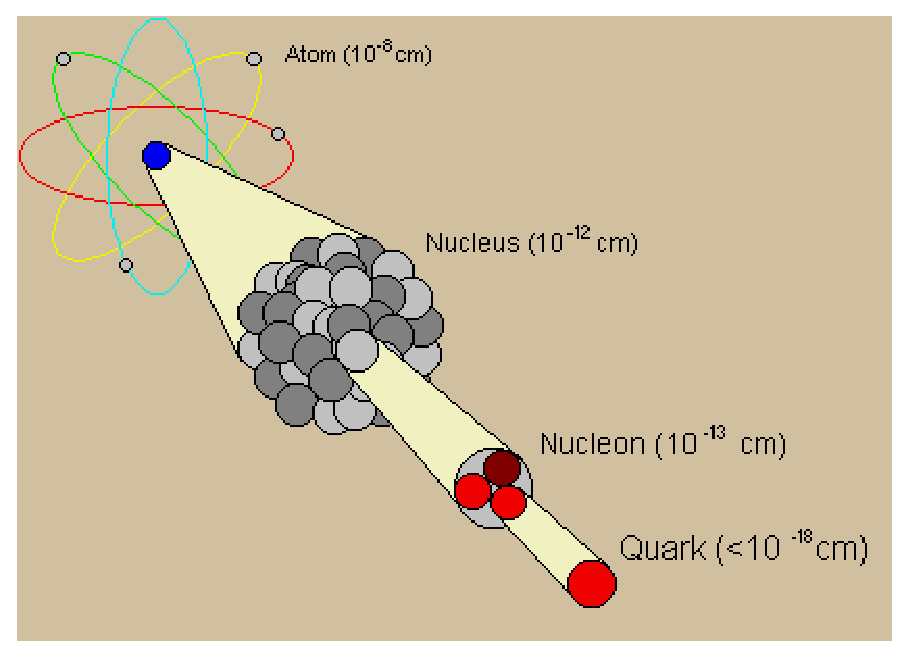
\includegraphics[type = eps, ext = .eps, scale = 1, bb = 0 0 420 300]{figs/atomo}
\end{slide}

\begin{slide}
\begin{center}
O Big-bang

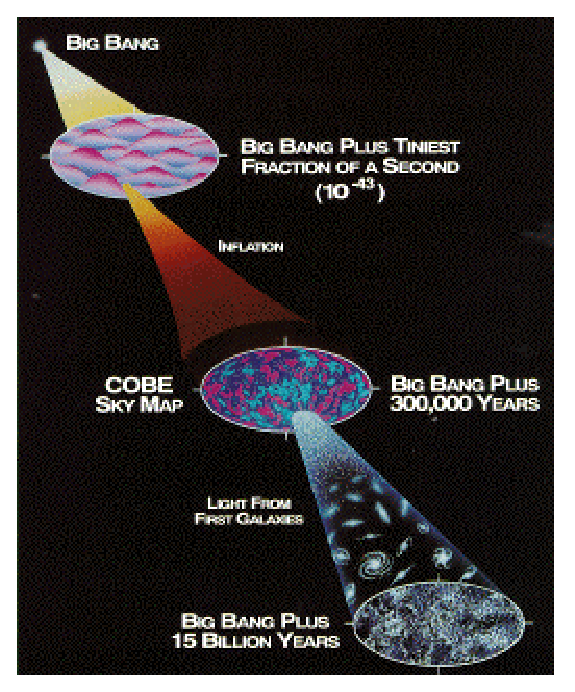
\includegraphics[type = eps, ext = .eps, scale = 1, bb = 0 0 260 316]{figs/bang}                

Os an�is aceleradores do CERN


\includegraphics[type = eps, ext = .eps, scale = 1, bb = 0 0 248 149]{figs/lhcair}
\end{center}
\end{slide}

\begin{slide}
O detetor ATLAS

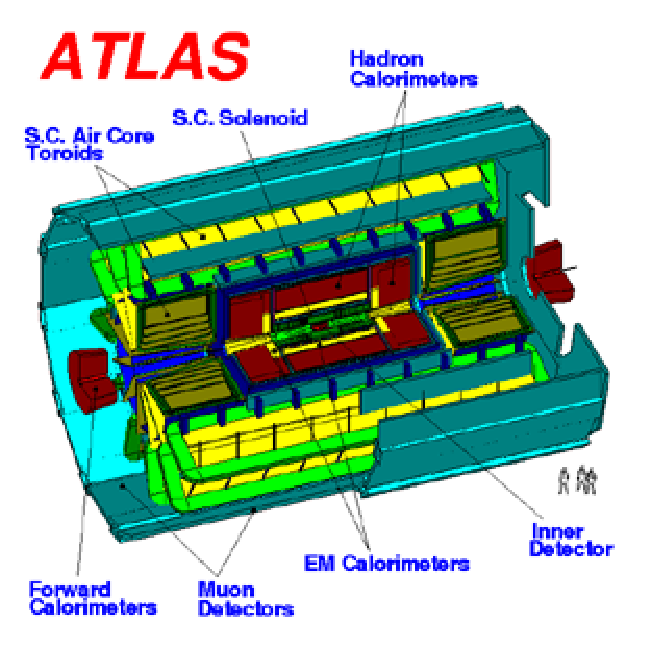
\includegraphics[type = eps, ext = .eps, scale = 1, bb = 0 0 300 295]{figs/atlasair}

Um evento reconstru�do

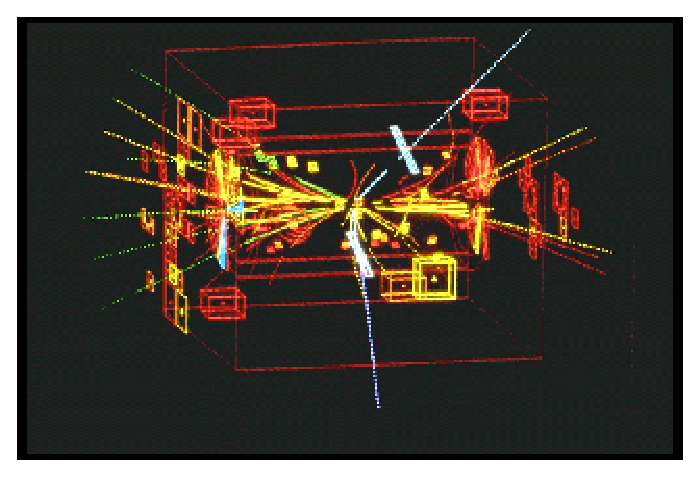
\includegraphics[type = eps, ext = .eps, scale = 1, bb = 0 0 320 213]{figs/colision}
\end{slide}

\begin{slide}
\begin{center}
Porque utilizar sistemas de valida��o ?

$\Downarrow$

Grande volume de dados

$\Downarrow$

\textcolor{blue}{\underline{Inviabilidade}} de armezenar tudo

$\Downarrow$

\textcolor{red}{\underline{Impossibilidade}} de faz�-lo
\end{center}
\end{slide}

\begin{slide}
O Sistema de \eng{Trigger} para o ATLAS

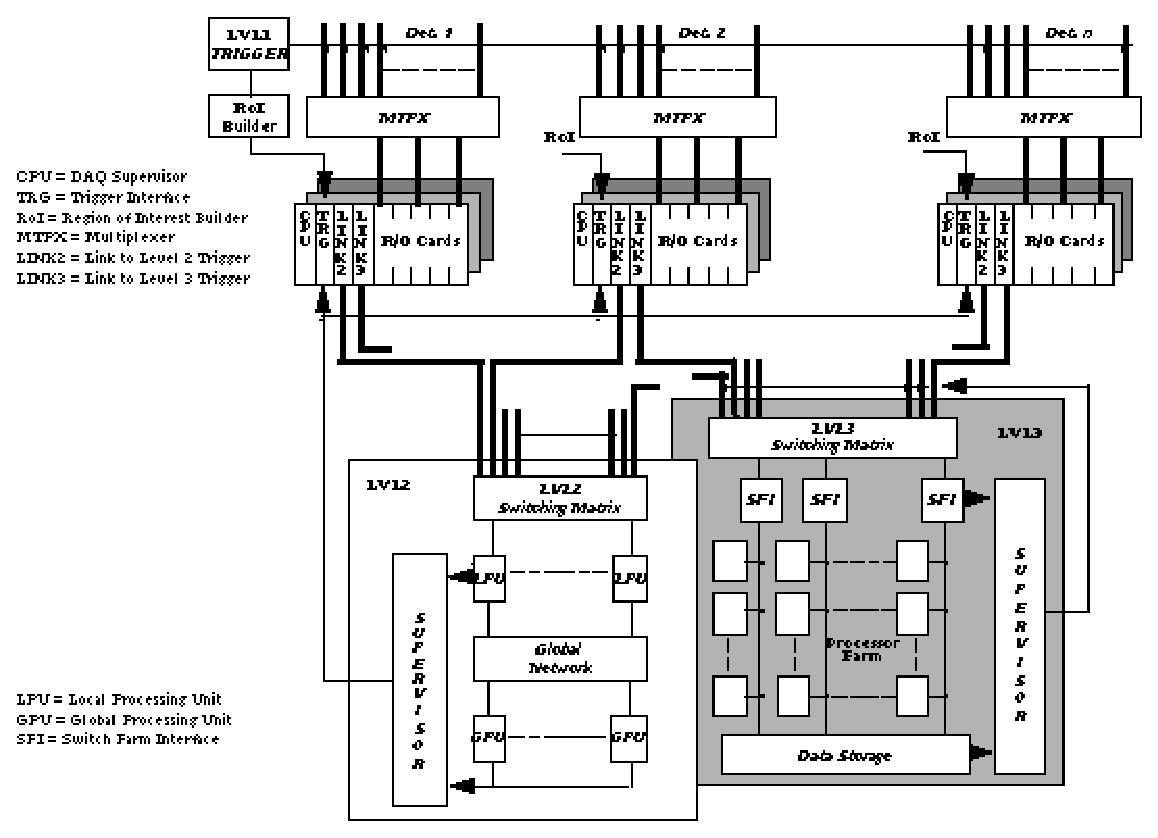
\includegraphics[type = eps, ext = .eps, scale = 0.8, bb = 0 0 540 386]{figs/trigger}
\end{slide}

\begin{slide}
Excitando os detetores

\input{picts/roi2.pic}
\end{slide}

\begin{slide}
A arquitetura A

{\tiny \input{picts/model_a2.pic}}
\end{slide}

\begin{slide}
A arquitetura B

{\tiny \input{picts/model_b2.pic}}
\end{slide}

\begin{slide}
A arquitetura C

{\tiny \input{picts/model_c2.pic}}
\end{slide}


 %% Whole introduction
\chapter{Revis�o da Literatura}
\label{chap:litera}
\index{Revis�o da Literatura}

Neste cap�tulo faremos a revis�o de algumas implementa��es e conceitos bem-sucedidos
 na descri��o e opera��o do 2\eiro n�vel de valida��o para o experimento ATLAS/LHC; 
destacam-se a utiliza��o de Redes Neurais como algor�tmo para alguns Extratores de 
Caracter�stica e unidades de Decis�o Global e, ainda, a utiliza��o de processamento 
paralelo em algumas implementa��es.

O motivo de tal direcionamento deste estudo deve-se � disponibilidade de 
equipamento com processamento distribu�do e bem-sucedidas implementa��es atrav�s de 
nosso grupo (Colabora��o Internacional CERN\-/\-COPPE\-/\-UFRJ) utilizando redes 
neurais artificiais na  
execu��o de extratores de caracter�sticas e unidades de decis�o global para a 
identifica��o de part�culas.

\section{Redes Neurais Artificiais e o processamento global para o segundo n�vel de
\eng{trigger}}
\index{Trigger!Level2!Redes Neurais aplicadas ao}
\index{Redes Neurais!Porque utiliz�-las no segundo n�vel de valida��o?}
\label{sec:ANN_at_globaldec}

Como elucidado na se��o~\ref{sec:level2}, o segundo n�vel de \eng{trigger} deve combinar as caracter�sticas 
vindas de diferentes subdetetores, de forma a aumentar a qualidade de classifica��o 
das part�culas. Neste est�gio � melhor n�o realizar uma identifica��o baseada em 
l�gica exclusiva, pois poderemos diminuir a qualidade de decis�o, mas gerar um outro 
conjunto de vari�veis, com probabilidades sobre a natureza da part�cula 
\cite{bock:ANN_at_level2}.

Considere o exemplo simples\index{Redes Neurais!Exemplo na classifi��o de 
part�culas} onde dois subdetetores n�o s�o correlacionados, ou 
seja, suas caracter�sticas extra�das s�o linearmente 
independentes (LI-s)\index{Independ�ncia Linear}. A forma mais ineficiente de 
fazer uma decis�o � a de classificar a part�cula segundo cada subdetetor e depois 
perfazer um ``E'' l�gico (AND) entre as classifica��es. Considere a ilustra��o 
da figura~\ref{fig:fexes} com as diferentes caracter�sticas extra�das da cada 
subdetetor (gen�rico), de tal forma que o n�vel de identifica��o para 2 tipos de 
excitadores de RoI, el�trons e jatos,  se d� com uma sobreposi��o de 10\%, o
 quer dizer que se tra�armos um corte para identifica��o em cada distribui��o 
teremos um erro m�nimo de 10\%. Neste exemplo a classifica��o exclusiva 
indicar� somente 81\% de corre��o na identifica��o das part�culas (o produto das 
probabilidades).

\begin{figure} 
 \begin{center}
 \caption{A distribui��o de caracter�sticas para cada subdetetor gen�rico. Os 
subsistemas s�o LI-s.} 
 \label{fig:fexes} 
 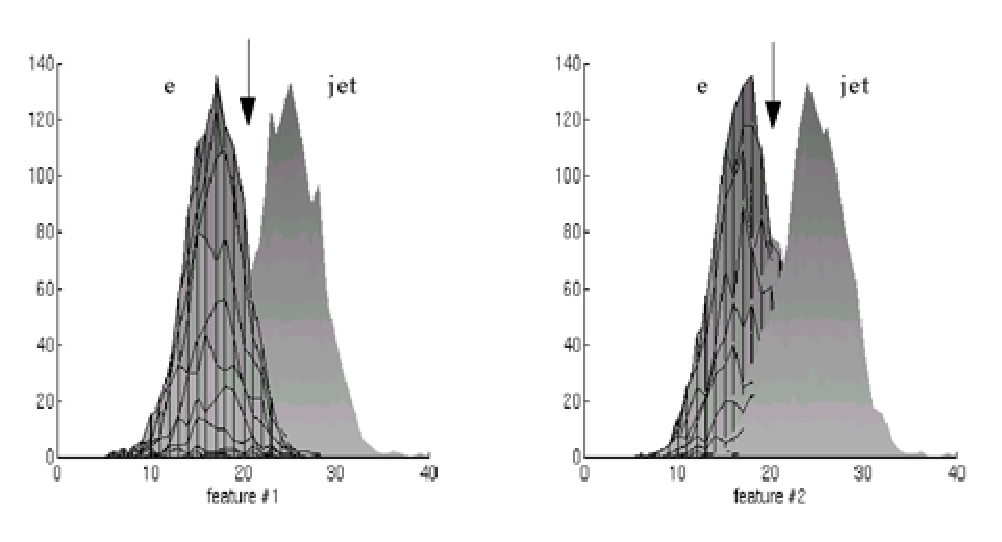
\includegraphics[type = eps, ext = .eps, scale = 0.9, bb = 0 0 464 243]{figs/fex_eg}
 \end{center}
\end{figure} 

A decis�o poder� ser melhor tomada se as duas caracter�sticas forem analisadas 
juntas, em um espa�o bidimensional (figura~\ref{fig:fex_bidim}). Cortando com um plano
como � mostrado, ambos os tipos de part�culas s�o 96\% corretamente classificadas. 
Estes tipos de cortes s�o realizados tamb�m por estruturas de Redes Neurais 
Artificiais utilizando a fun��o identidade como a fun��o de transfer�ncia para 
os neur�nios. Se o n�mero de subdetetores crescer, a diferen�a entre estas duas 
maneiras de classifica��o ficar� mais expl�cita, como � poss�vel observar na 
tabela~\ref{tab:efici_ann}. Neste teste foi considerado que todas as caracter�sticas 
foram extra�das de subsistemas LI-s, assim sendo, n�o houve necessidade da utiliza��o de
camadas escondidas.

\begin{figure} 
 \begin{center}
 \caption{Exemplo de classifica��o num espa�o bidimensional} 
 \label{fig:fex_bidim} 
 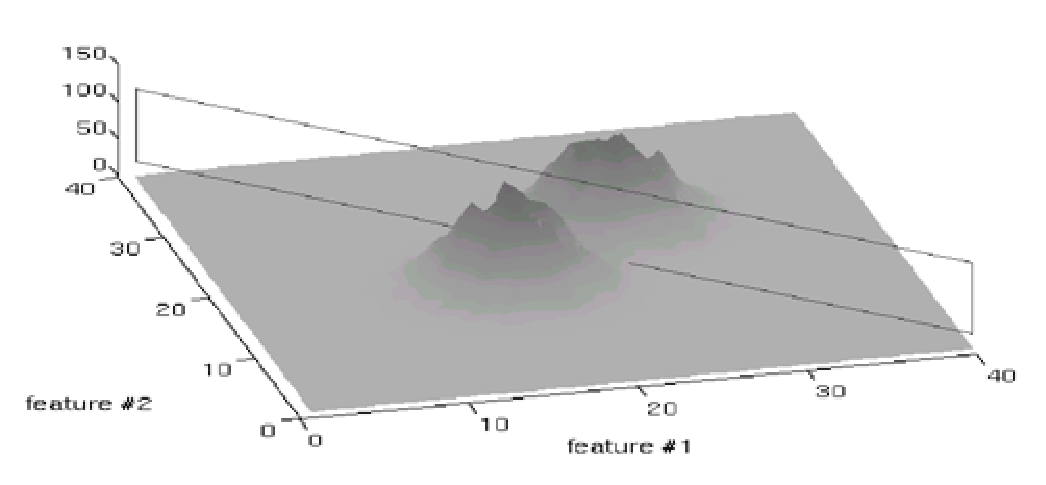
\includegraphics[type = eps, ext = .eps, scale = 0.85, bb = 0 0 485 216]{figs/fex_bid}
 \end{center}
\end{figure} 

\begin{table}
 \begin{center}
 \caption{Tabela de efici�ncias para uma classifica��o utilizando um ``E'' l�gico e 
Redes Neurais Artificiais simples, sem camadas escondidas.}
 \label{tab:efici_ann}
 \begin{tabular}{|c||c|c|}
 \hline
 N�mero de Detetores & Classifica��o com ``E'' l�gico & Classifica��o com ANN \\ 
 \hline \hline
 1 & 90\% & 90\% \\ \hline 
 2 & 81\% & 96.5\% \\ \hline 
 3 & 73\% & 98.8\% \\ \hline 
 4 & 65\% & 99.4\% \\ \hline 
 5 & 59\% & 99.8\% \\ \hline 
 \end{tabular}
 \end{center}
\end{table}\index{Redes Neurais!Tabela comparativa com se\-pa\-ra\-��o cl�s\-si\-ca}

Embora pare�a simples, a tarefa para a identifica��o de part�culas � um processo 
que envolve caracter�sticas extra�das dos dados de um n�mero de subdetetores menor 
que o n�mero de caracter�sticas\footnote{O n�mero de detetores est� entre 4 e 6 e o 
de caracter�sticas, entre 12 e 15.}, portanto, algumas destas s�o linearmente 
dependentes (LD-s)\index{Depend�ncia Linear}. Para m�xima efici�ncia na separa��o com vari�veis LD-s a 
utiliza��o de camadas escondidas � necess�ria. A figura~\ref{fig:LD_vars_and_ANNS} 
mostra o resultado de separa��o obtida sobre dados LD-s utilizando 3, 2 ou nenhum 
neur�nio na camada escondida.

\begin{figure} 
 \begin{center}
 \caption{Classifica��o em um espa�o de vari�veis linearmente dependente.} 
 \label{fig:LD_vars_and_ANNS} 
 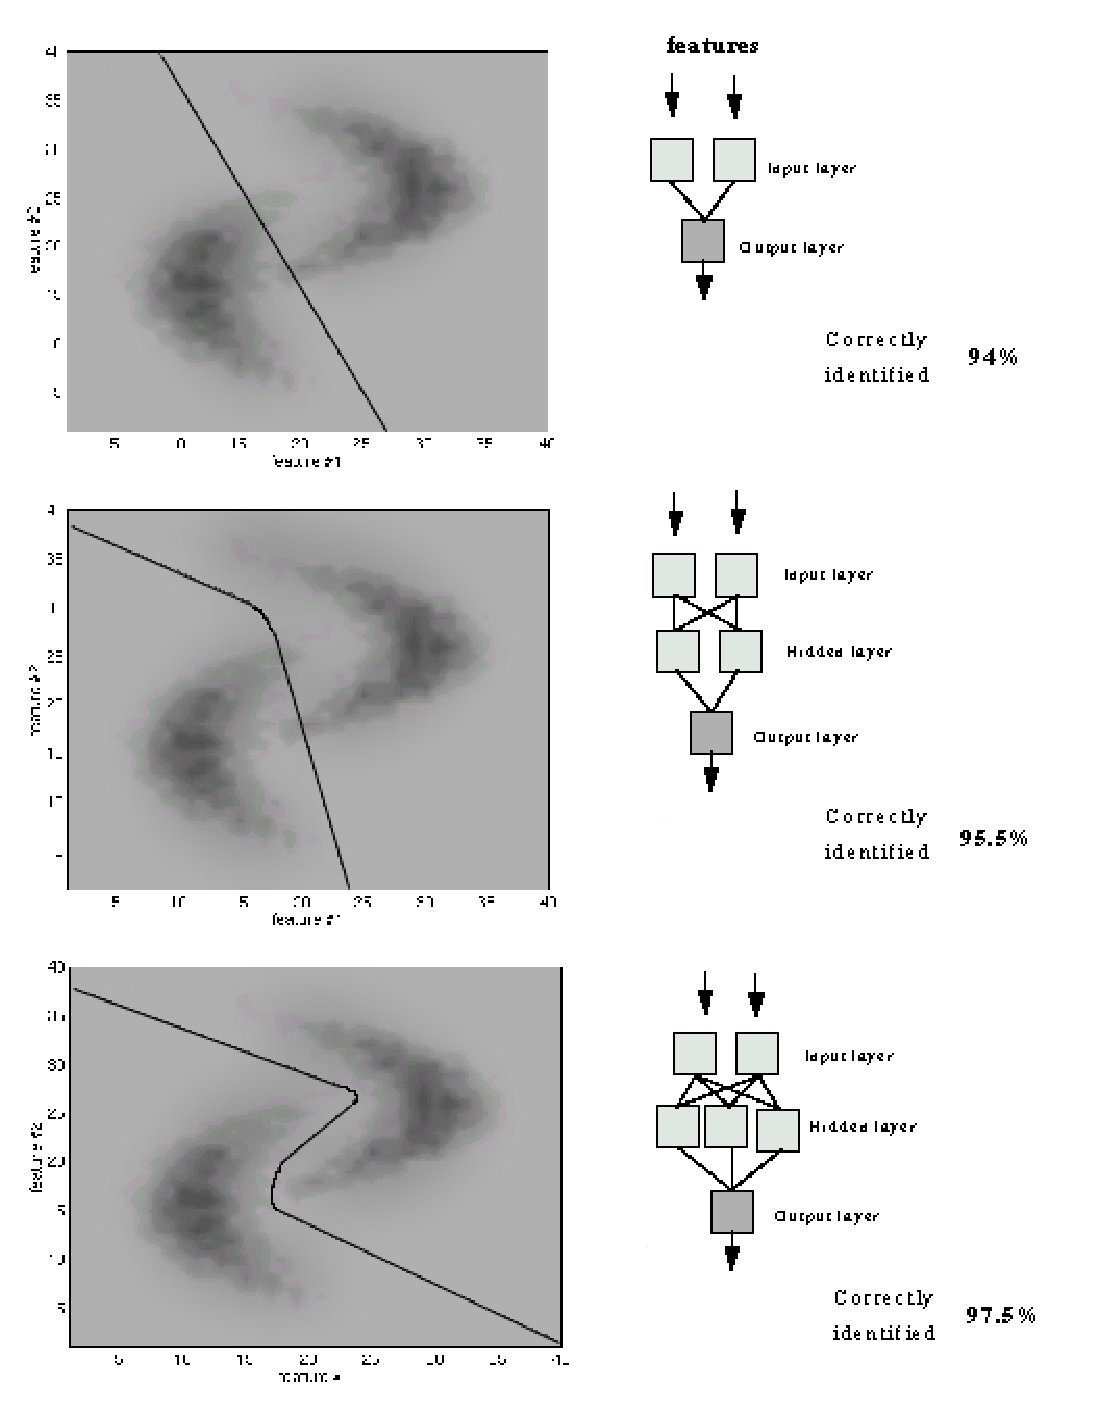
\includegraphics[type = eps, ext = .eps, scale = 0.8, bb = 0 0 511 661]{figs/annhid}
 \end{center}
\end{figure} 

\paragraph{Conclus�o:} O processamento de Decis�o Global ter� �tima efici�ncia se 
utilizarmos Redes Neurais Artificiais (ANN-s) ao inv�s de algoritmos basedos em 
classifica��o exclusiva, devido ao n�mero de subsistemas e vari�veis envolvidas. Em 
raz�o da depend�ncia entre as vari�veis dos diversos subsistemas parece inevit�vel 
a utiliza��o de ao menos uma camada escondida em uma rede neural simples, 
diretamente conectada (\eng{feed forward}).

Em particular, resultados com redes na configura��o 12-6-4, isto �, 12
entradas, 6 neur�nios na camada escondida e 4 na de sa�da t�m se mostrado satisfat�rios onde
tempo de processamento e efici�ncia s�o fatores dominantes como � poss�vel ver em 
\cite{sx:gldec}. O n�mero de sa�das � fortemente dependente da quantidade de 
part�culas diferentes que se deseja identificar no processamento da RoI. No 
caso espec�fico supracitado a identifica��o se fez por uma separa��o entre 4 
diferentes tipos de part�culas (el�trons, jatos, p�ons e m�ons).

Devemos destacar ainda que redes neurais s�o capazes de encontrar correla��es em 
espa�os multi-dimensionais ainda que na presen�a de grande quantidade de ru�do. 
Redes Neurais artificiais tamb�m podem ser muito competitivas onde pre�o e robustez 
s�o fatores delimitantes.

\section{A utiliza��o de ambientes de processamento distribu�do para o segundo n�vel de
 \eng{trigger}}
\index{Paralelismo!Porque utilizar?}

Devido �s altas taxas de eventos a que ser� submetido o segundo n�vel de 
\eng{trigger} (muitos Gigabytes por segundo e uma lat�ncia m�xima presumida de 1ms), a 
decomposi��o do problema atrav�s de paraleliza��o das atividades 
parece apontar um caminho para a solu��o. Esta
paraleliza��o pode ser implementada em 2 n�veis:
\begin{enumerate} 
 \item Na paraleliza��o de uma atividade simples como a extra��o de uma 
caracter�stica ou a identifica��o de uma part�cula, de modo a reduzir a lat�ncia do 
processamento localizado; e
 \item Na paraleliza��o de uma classe de atividades ou de todo o processamento para 
este n�vel, por exemplo, a extra��o de 
caracter�sticas utilizando uma \eng{farm} de processadores operando em paralelo 
sobre dados de diferentes RoI-s, reduzindo a lat�ncia do processamento como um todo e
 n�o localmente como no item anterior.
\end{enumerate}

Os dois tipos de paraleliza��o levam a diferentes enfoques de 
implementa��o\index{Paralelismo!enfoques}: no 
primeiro teremos um algoritmo baseado na taxa de dados (\eng{Data 
Driven})\index{Paralelismo!Data
Driven Approach}  de entradab visto que a 
paraleliza��o � feita de modo a reduzir as lat�ncias individuais, reduzindo  
a lat�ncia global do processo para cada evento. Nesta implementa��o deve-se utilizar  
uma arquitetura capaz de sustentar a taxa de dados, como em 
\cite{bock:cpp_at_level2}.

No segundo enfoque, a lat�ncia dos processos individuais n�o � demasiado importante, 
visto que poderemos compensar uma maior lat�ncia com a utiliza��o de mais 
processadores naquele n�vel de processamento. Este tipo de implementa��o � conhecido
 como \eng{Asynchronous Processor Farms 
Implementation}\index{Paralelismo!Asynchronous Approach} ou Implementa��o em 
\eng{farms} de processadores ass�ncronos. O assincronismo vem do fato das atividades
 paralelas serem independentes quanto ao tempo de execu��o entre si, podendo ser 
executadas totalmente livres do final (ou come�o) de processamento de qualquer evento
ou dado em qualquer outra unidade de processamento.

No caso do segundo n�vel em espec�fico\index{Paralelismo!Para o segundo n�vel}, 
podemos enxergar paralelismo em  
algumas das atividades realizadas e no processamento como um todo tamb�m. Para 
algoritmos de extra��o de caracter�sticas em calor�metros, t�cnicas de processamento 
paralelo  
ass�ncrono t�m se mostrado eficientes no atendimento das taxas de entrada do 
experimento, como � poss�vel ler em \cite{sx:fe}. 

Para as unidades de Decis�o Global, a utiliza��o de redes neurais artificiais t�m 
mostrado vantagem, como explicita a se��o~\ref{sec:ANN_at_globaldec}. Redes Neurais 
s�o algoritmos altamente paraleliz�veis por serem baseados em multiplica��es e somas 
vetoriais totalmente independentes ao n�vel de cada camada\footnote{� claro que os 
resultados da camada de ordem $n$ dependem dos resultados da camada de ordem 
$n-1$ e, sendo assim, n�o podemos tornar isto concorrente, ou seja, o processamento 
ainda deve ser feito camada a camada.}. Ainda, otimiza��es podem ser realizadas a 
n�vel ass�ncrono utilizando-se mais de uma rede para o processamento global.

Por fim, as atividades do segundo n�vel como um todo s�o paraleliz�veis visto a 
independ�ncia entre diferentes eventos. Estes podem ser processados 
independentemente (e, desta forma, ass�ncronamente) uns dos outros, sem perda 
de informa��es, de forma que a lat�ncia 
para cada evento possa ser aumentada proporcionalmente do valor alvo de 1ms para 
outro valor maior, dependendo de quantos forem os n�s de processamento adicionados. 
Este enfoque,  
� claro, reduz a necessidade de otimiza��o dos subn�veis de processamento internos 
ao segundo n�vel, como � o caso do enfoque baseado na taxa de dados (\eng{Data Driven 
Approach}).

\subsection{DSP-s}
\index{DSP-s!Utilidade}

\eng{Digital Signal Processors} (processadores digitais de sinais) n�o s�o mais do 
que r�pidos processadores matem�ticos que executam fun��es aritm�ticas b�sicas e 
outras fun��es complexas com poucos pulsos de \eng{clock}. Alguns DSP-s como o 
ADSP-21020 da Analog Devices podem processar em apenas 1 ciclo de \eng{clock} uma multiplica��o 
entre n�meros reais(ou pontos flutuantes).

Vantagens na utiliza��o de DSP-s s�o expl�citas quando o processamento depende do 
c�lculo de muitas vari�veis. No caso do processamento para o segundo 
n�vel, existem muitos subn�veis em que � poss�vel atingir uma redu��o da lat�ncia de
processamento utilizando-se DSP-s como processadores centrais do subn�vel \cite{bock:cpp_at_level2}.
Este � o caso da maioria dos extratores de caracter�stica e das unidades de decis�o 
global, se desenhados como Redes Neurais Artificiais.

\section{Arquiteturas para o segundo n�vel de \eng{trigger}}
\index{Trigger!Level2!Arquiteturas}

Limita��es de tamanho e custo podem nos levar a 3 poss�veis arquiteturas mutuamente 
exclusivas para o segundo n�vel de processamento\cite{level2:tsr}:
\begin{itemize} 
 \item{\bf Modelo A:} Utiliza uma parti��o local/global do segundo n�vel de processamento, 
com processamento at� a extra��o de caracter�sticas (inclusive) sendo realizado com 
arquitetura baseda no 
enfoque \eng{data-driven}, enquanto que o processamento global utiliza uma \eng{farm}
 de processadores utilizando o enfoque de processamento ass�ncrono;
 \item{\bf Modelo B:} Utiliza uma parti��o local/global de todo o processamento do 
segundo n�vel, fazendo uso de v�rias \eng{farms} feitas de processadores id�nticos ou
similares com extra��o de caracter�sticas paralela para cada subdetetor e para cada
RoI;
 \item{\bf Modelo C:} Uma �nica \eng{farm} de processadores realizando, cada um, o 
processamento relativo a um evento inteiro.
\end{itemize}

Estas arquiteturas seguem alguns crit�rios de funcionamento tais como n�o possuir 
lat�ncia de opera��o\footnote{Tempo de demora entre a decis�o do 1\eiro n�vel e a 
decis�o do segundo.} superior a 2 ms (modelo A) e 10 ms (modelos B e C); caso esta 
ultrapasse, o supervisor deve se responsabilizar por abortar a opera��o de valida��o 
para este evento. Estes crit�rios podem ser melhor estudados em 
\cite{level2:tsr} e \cite{level2:urd}.

\subsection{Modelo A}
\index{Trigger!Level2!Arquiteturas-Modelo A}

Neste modelo A, a informa��o de cada RoI � comunicada pelo \eng{RoI Builder} �s 
ROB-s (isto ainda � no 1\eiro n�vel). Os dados s�o ent�o ``empurrados'' atrav�s do 
pr�-processamento e cole��o de RoI-s para a extra��o de caracter�sticas. Nesta parte
de opera��o as unidades de processamento (acopladas, formando um �nico subsistema) 
dever�o suportar a mais alta taxa de eventos poss�vel. As opera��es s�o totalmente 
independentes para os dados de diferentes subdetetores. Para cada RoI, um vetor de 
dados � preparado contendo as caracter�sticas extra�das e um cabe�alho de 
identifica��o. Depois da extra��o de caracter�sticas, estes vetores s�o encaminhados
 a uma chave que � respons�vel por distribu�-los pelos processadores globais. A 
figura~\ref{fig:mod_a} pode ser elucidativa quanto ao mencionado nesta se��o.

\begin{figure} 
 \begin{center}
 \caption{Um diagrama esquem�tico para o modelo arquitetural A do segundo n�vel de 
valida��o.} 
 \label{fig:mod_a} 
 \input{picts/model_a.pic}
 \end{center}
\end{figure} 

\subsection{Modelo B}
\index{Trigger!Level2!Arquiteturas-Modelo B}

Neste modelo B, a informa��o de cada RoI � passada ao supervisor que controla {\bf 
todo} o fluxo de dados. Os dados de cada RoI s�o passados dos ROB-s atrav�s do 
pr�-processamento e cole��o de RoI-s a uma chave que se encarrega de passar os dados
 relativos a cada RoI para extratores de caracter�sticas. Nesta fase, os subsistemas
 relativos a cada subdetetor s�o totalmente independentes, podendo ter seus pr�prios
 supervisores locais. As caracter�sticas 
extra�das s�o, ent�o, passadas atrav�s de outra chave (que re�ne as caracter�sticas 
extra�das de cada subdetetor sobre uma mesma RoI), que repassa estes dados �s 
unidades de decis�o global. A figura~\ref{fig:mod_b} mostra um diagrama ilustrativo.

\begin{figure} 
 \begin{center}
 \caption{Um diagrama esquem�tico para o modelo arquitetural B do segundo n�vel de 
valida��o.} 
 \label{fig:mod_b} 
 \input{picts/model_b.pic}
 \end{center}
\end{figure} 

\subsection{Modelo C}
\index{Trigger!Level2!Arquiteturas-Modelo C}

Neste modelo C, a informa��o � passada a um supervisor central que dedica um dos 
processadores de uma \eng{farm} homog�nea a todo o processamento do evento. Este 
processador controla todo o fluxo de dados da RoI pelos ROB-s e pelas unidades de 
pr�-processamento e cole��o de RoI-s. Os dados, depois de coletados, seguem a uma 
chave que os repassa ao devido processador de evento, para que este realize a extra��o
 de caracter�sticas e a decis�o global. A figura~\ref{fig:mod_c} mostra um diagrama 
ilustrativo.

\begin{figure} 
 \begin{center}
 \caption{Um diagrama esquem�tico para o modelo arquitetural C do segundo n�vel de 
valida��o.} 
 \label{fig:mod_c} 
 \input{picts/model_c.pic}
 \end{center}
\end{figure} 

\section{Concluindo alguns pontos...}
\index{Revis�o da Literatura!conclus�o}

� poss�vel utilizar ANN-s para desenhar alguns subsistemas do segundo n�vel de 
valida��o, em especial Unidades de Decis�o Global e Extratores de Caracter�sticas 
para Calor�metros. Estas redes especializadas no reconhecimento de padr�es podem ter sua 
lat�ncia reduzida se utilizarmos computa��o distribu�da uma vez que seu algoritmo � 
altamente paraleliz�vel. Ainda, se utilizarmos DSP-s como processadores centrais de 
alguns destes subsistemas poderemos nos beneficiar de sua alta performance 
computacional em algoritmos envolvendo repetidos c�lculos.

A paraleliza��o da aplica��o (ainda que complexa) poder� acontecer em 2 inst�ncias: 
na primeira,  
local, h� uma paraleliza��o buscando a otimiza��o de um algoritmo utilizado em 
um subsistema, de forma a atender �s taxas de entrada e lat�ncia m�ximas deste 
subsistema; chamamos este enfoque de \eng{data-driven} uma vez que os dados fluir�o 
por estes subsistemas sem restri��es ou controle, j� que estes suportar�o as taxas de 
entrada m�ximas. Na segunda inst�ncia, global, acontece uma paraleliza��o de subsistemas 
id�nticos (exemplo: Extratores de Caracter�stica) de forma que a lat�ncia m�xima para
cada evento seja aumentada proporcionalmente ao n�mero de processadores 
anexados. Em particular a paraleliza��o em primeira inst�ncia n�o ser� aqui 
utilizada visto que equipamento espec�fico para cada subsistema paraleliz�vel � 
requerido. Utilizaremos, no entanto, o conceito de paraleliza��o global, 
ou em segunda inst�ncia como veremos mais a frente.

Existem v�rios modelos para a implementa��o do segundo n�vel, cada um com suas 
vantagens e desvantagens, embora de uma forma geral bem plaus�veis. Para fins 
e objetivos deste projeto, no entanto, nos concentraremos no modelo B. O modelo A 
requer utiliza��o de processamento  
diversificado para a camada de pr�-processamento, cole��o de RoI-s e Extra��o de 
Caracter�sticas, o que n�o ser� poss�vel, pois somente dispomos de 16 processadores em 
nossa m�quina (v�-la-emos em detalhes mais adiante) que ter�o seus potenciais 
subaproveitados se os utilizarmos em uma paraleliza��o local ou em primeira 
inst�ncia.

O modelo C exige um chaveamento a partir dos ROB-s utilizando uma chave muito r�pida
(tecnologia ATM), que tamb�m n�o se encontra em nosso poder. A arquitetura B, no 
entanto, nos  
parece mais adpt�vel ao equipamento dispon�vel (TELMAT TN310) e que queremos 
avaliar; sendo assim, 
tentaremos abordar o problema e construir o simulador baseado neste desenho. 
Lembramos que queremos atingir 2 metas aqui: a primeira � construir um 
sistema de valida��o, a segunda, testar a tecnologia contida em uma TN310 de 
forma a avaliar globalmente arquitetura e equipamento para a realiza��o do segundo 
n�vel de valida��o para o experimento ATLAS\-/\-LHC.
 
No que se segue exporemos em detalhes alguns dos conceitos, materiais e m�todos 
utilizados neste projeto, isto �, Redes Neurais Artificiais, a m�quina 
mencionada - Telmat TN310, os dados utilizados e alguns conceitos de paralelismo.

 %% Documentation Revision
%% This file contains 6 slides
\begin{slide}
Redes Neurais Artificiais - O neur�nio artificial

\begin{center}
{\tiny \input{picts/neuronc.pic}}
\end{center}
RNA multi-camadas

\begin{center}
{\tiny \input{picts/multi.pic}}
\end{center}
\end{slide}

\begin{slide}
O Sistema TN310

\begin{itemize} 
 \item Processamento Distribu�do
 \item 16 n�s independentes
 \item Mem�ria Local (MIMD)
 \item HTRAM-s tamanho 4
 \begin{enumerate} 
  \item T9000
  \item ADSP 21020 (196Kbytes)
  \item 8Mbytes RAM
  \item 256Kbytes \eng{shared}
 \end{enumerate}
 \item Totalmente conectado atrav�s de chaves STC104
\end{itemize}
\end{slide}

\begin{slide}
O T9000

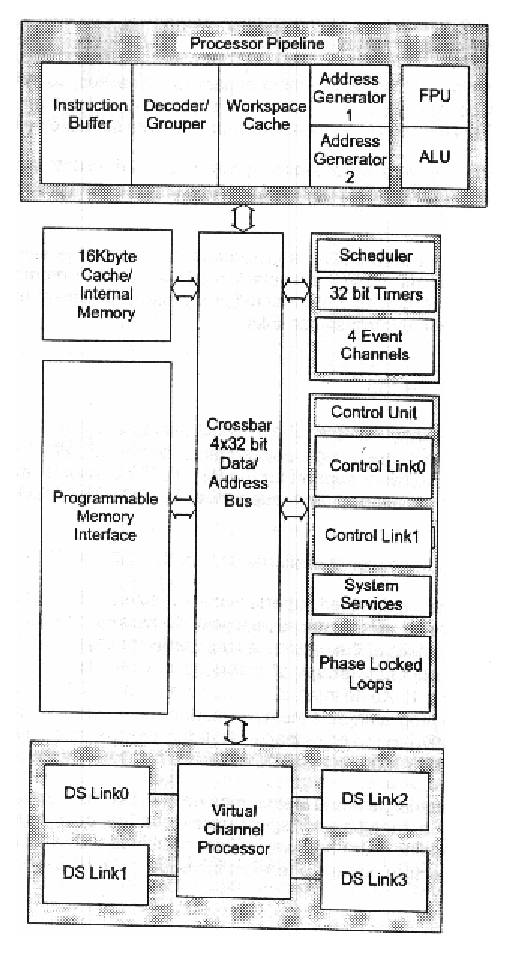
\includegraphics[type=eps, ext=.eps, bb= 0 0 228 441]{figs/T9000}
\end{slide}

\begin{slide}
O ADSP 21020

\end{slide}

\begin{slide}
A conex�o entre os n�s na TN310

{\tiny \input{picts/connect2.pic}}
\end{slide}

\begin{slide}
N�veis de programa��o

\begin{center}
{\tiny \input{picts/layer.pic}}
\end{center}

Comunica��o por canais
\begin{center}
{\tiny \input{picts/chan_op2.pic}}
\end{center}
\end{slide}


 %% Theoretical Fundaments, Methods and Materials used at this project
%% This file contains 9 slides
\begin{slide}
Modelo de neur�nio utilizado

\begin{center}
{\tiny \input{picts/neuronc.pic}}
\end{center}

A rede para a GDU
\begin{center}
{\tiny \input{picts/gdu_net.pic}}
\end{center}
\end{slide}

\begin{slide}
\begin{center}
Tabela de convers�o

{\tiny \input{picts/lut_ex2.pic}}

GDU em paralelo

{\tiny \input{picts/gdu_full.pic}}
\end{center}
\end{slide}

\begin{slide}
A comunica��o com os escravos

{\tiny \input{picts/shake.pic}}

O supervisor (fluxograma)
z
\begin{center}
{\tiny \input{picts/sup_flow.pic}}
\end{center}
\end{slide}

\begin{slide}
{\small
Resultados para a GDU
\begin{itemize} 
 \item O tempo de processamento para uma RoI da GDU rodando em apenas 1 n� � de 200$\mu$s
 \item Alocando o supervisor no n� zero e 15 escravos o tempo de processamento por 
RoI � de 30,3$\mu$s (\eng{speed-up} = 6.6)
 \item Alocando o supervisor no n� 15 e 15 escravos o tempo de processamento cai 
para 27$\mu$s (\eng{speed-up} = 7.4)
\end{itemize}
Conclus�es
\begin{itemize} 
 \item Tabela de convers�o � eficiente - reduzimos o tempo de processamento sem 
perder efici�ncia
 \item A aloca��o ``inteligente'' de tarefas leva a melhores resultados
 \item \eng{speed-up} - Bom desempenho, mas � o m�ximo ? 
\end{itemize}}
\end{slide}

\begin{slide}
� implementar no 2\eiro n�vel

{\tiny \input{picts/mod_bi2.pic}}
\end{slide}

\begin{slide}
Generaliza��o

\begin{center}
{\tiny \input{picts/top_tn.pic}}
\end{center}
\end{slide}

\begin{slide}
\label{slide:implementa}
Implementa��o usando os 16 n�s

{\tiny \input{picts/sim_v2a2.pic}}
\end{slide}

\begin{slide}
Resultados para a vers�o em apenas 1 n�
\begin{itemize} 
 \item N�o leva em considera��o tempo de distribui��o (necess�rio)
 \item Tempo para uma RoI = 1320$\mu$s
\end{itemize}
Resultado para a vers�o concorrente 1 (aloca��o aleat�ria)

$\Rightarrow$ Tempo para uma RoI = 830$\mu$s (\eng{speed-up} = 1,6)

Resultado para a vers�o concorrente 2 (aloca��o ``inteligente'')

$\Rightarrow$ Tempo para uma RoI = 690$\mu$s (\eng{speed-up} = 1,9)

Resultados para a vers�o concorrente 3 (distribui��o sequencial)

$\Rightarrow$ Tempo para uma RoI = 390$\mu$s (\eng{speed-up} = {\bf 3,4 !})
\end{slide}

\begin{slide}
Conclus�es
\begin{itemize} 
 \item Sabendo que \eng{speed-up} m�ximo � 4 ($//$ dados e fluxo) atingimos 85\% do 
m�ximo
 \item Melhora de 43\% da vers�o 3 para a vers�o 2
 \item Considerando 1 e\-ven\-to $\approx$ 5 RoI-s $\Rightarrow$ 2ms\-/\-e\-ven\-to (500Hz)
 \item Lentid�o $\Rightarrow$ Tempo de distribui��o dos dados para fex-s $\Rightarrow$ 96\% do 
tempo total de aplica��o
 \item Atingimos o m�ximo desta tecnologia ?
\end{itemize}
\end{slide}

 %% Project implementation and constraints at TN310
\chapter{Resultados obtidos e Conclus�es}
\label{chap:results}

Neste cap�tulo, estaremos expondo os resultados obtidos com as implementa��es expostas
no cap�tulo anterior. Para todas as implementa��es, consideramos o \eng{speed-up} em 
rela��o a uma vers�o simples da aplica��o, isto �, rodando em um �nico processador. 
Tamb�m � feita uma revis�o dos tempos de comunica��o e afins.

Inicialmente, repassaremos testes realizados sobre o tempo de comunica��o do sistema 
TN310. Estes testes visaram a um entendimento operacional do tempo de processamento 
dispendido durante comunica��es entre aplica��es. Na segunda se��o, traremos 
resultados para a aplica��o do sistema de decis�o global e na se��o seguinte, 
exporemos os resultados e conclus�es para a simula��o do sistema de valida��o.

\section{Teste de comunica��es}
\secl{time}

Em equipamentos com n�mero de n�s de processamento consider�vel � necess�rio o 
entendimento pleno do sistema de comunica��o utilizado. Quando menciona-se 
``Entendimento Pleno" quer se acentuar que para uma otimiza��o das rotinas h�
 a necessidade de o programador desenvolver uma ``afinidade'' muito grande com o 
equipamento. Esta afinidade traduz-se no entendimento de todos os detalhes de 
funcionamento do sistema, sejam eles de alto ou de baixo n�vel.

O processo de comunica��o entre os diversos n�s de processamento no sistema TN310 
n�o � diferente,  
isto �, ele possui uma interface de alto n�vel (como as fun��es da 
tabela~\tabr{channel.h}) e uma interface de baixo n�vel, inerente ao sistema. A 
interface de alto n�vel � respons�vel pelo processo de comunica��o em si, mas os 
motivos pelos quais alguns tipos de comunica��o s�o diferentes de outros � um ponto 
que somente pode ser explicado com o entendimento do sistema operando em baixo 
n�vel. Desta forma, antes de entrarmos nos resultados destes testes propriamente,
abordaremos alguns aspectos na forma de comunica��o entre os diversos n�s HTRAM do 
sistema TN310.

\subsection{Introdu��o ao sistema de comunica��es}

O sistema de comunica��es da TN310 � totalmente baseado no conceito de chaveamento 
ass�ncrono de pacotes (\eng{Asynchronous Packet Switch}). Este tipo de sistema pode 
aumentar a ``performance'' em ambientes maiores, como � caso. Ele se baseia na utiliza��o
 de uma chave r�pida (STC104) para que haja a distribui��o de pacotes pela rede de 
forma mais r�pida e livre de erros poss�vel. Estas chaves podem rotear at� 32 
pacotes diferentes ao mesmo tempo, vindo de quaisquer 32 localidades distintas e 
indo para outras 32 localidades tamb�m distintas.

A id�ia �, na verdade, bem simples. Quando uma informa��o deseja ser mandada de um 
ponto a outro, a tarefa no ponto emissor envia uma mensagem ao processador virtual de
 canais local indicando o endere�o e o tamanho do dado a ser mandado. O processador 
de canais divide o dado a ser enviado em v�rios pacotes de tamanho predeterminado. 
Ap�s esta divis�o, a cada pacote � adicionado um cabe�alho contendo a loca��o-destino 
e a rota para o pacote. O pacote � enviado a uma chave que interpreta a primeira parte do 
cabe�alho e envia o pacote para o n� correto, removendo a parte do cabe�alho 
referente � rota j� informada e deixando exposta a parte do cabe�alho referente ao 
n�-destino do pacote. Ao chegar ao n�-destino,
cada pacote � autenticado (i.e., verifica-se se realmente se est� esperando 
tal informa��o e se o cabe�alho est� correto) e um reconhecimento (\eng{acknowledgement}) 
� enviado para que o pr�ximo pacote seja mandado, se este for o caso.

No caso de o pacote ter que passar por 2 chaves, 3 cabe�alhos s�o inseridos a cada 
pacote. Este ser� roteado atrav�s de 2 chaves e ocorrer�o 2 remo��es de 
cabe�alhos (\eng{header deletion}) e apenas um ser� utilizado novamente no n� destino.
Desta forma, � poss�vel garantir que poderemos criar um n�mero muito grande de 
canais virtuais. Comunica��o utilizando canais virtuais nada mais � do que 
comunica��o feita com pacotes de dados  intercalados simulando um sistema com maior 
n�mero de conex�es do que realmente existem.

Quando � dito que h� uma multiplexa��o dos canais, quer-se dizer que, uma
vez que s�o dividos em pacotes, os dados a serem enviados podem ser intercalados, 
gerando uma rede de multiplexa��o de pacotes e, assim, satisfazendo um grande n�mero 
de canais simult�neos, chamados virtuais. 

A figura~\figr{header_del} pode ser elucidativa quanto � remo��o de cabe�alhos.

\begin{figure} 
 \begin{center}
 \caption{O processo de dele��o de cabe�alho em uma rede com chaveamento ass�ncrono 
de pacotes.} 
 \figl{header_del} 
 \input{picts/head_del.pic}
 \end{center}
\end{figure} 

\paragraph{Concluindo.} A TN310 � um sistema distribu�do com 16 n�s de processamento
tipo HTRAM totalmente conectados atrav�s de uma rede de chaves ass�ncronas. A 
comunica��o nesta rede � feita atrav�s canais descritos em \eng{software} (InMOS C), mas
implementados via \eng{hardware} atrav�s de um sistema de canais virtuais cujo 
processador central � o VCP (Processador de Canais Virtuais). O VCP divide a 
informa��o a ser mandada em pacotes e a cada pacote adiciona um n�mero de cabe�alhos
proporcional ao n�mero de n�s por onde o pacote passar�. Assim sendo, se o pacote 
tiver que passar por 2 chaves adicionar-se-�o 3 cabe�alhos (2 para as chaves e 1 para 
o n�-destino). Os pacotes s�o enviados intercaladamente com outros pacotes de outras
informa��es que tamb�m est�o sendo enviadas. Isto cria uma rede de canais virtuais.

\subsection{Os testes}

Levando em considera��o que estaremos alocando em cada n� de processamento uma �nica
tarefa seq�encial, isto �, sem que dispare processos concorrentes, podemos chegar � 
conclus�o que todos os DS-Links estar�o � disposi��o da aplica��o para a transmiss�o
de dados. Isto maximiza a utiliza��o dos meios de comunica��o de cada n�. Estamos 
interessados em entender 2 pontos na opera��o do sistema:
\begin{enumerate} 
 \item Qual � o tamanho de cada pacote mandado por vez?
 \item Quanto tempo demora para que pacotes sejam enviados a diferentes n�s de 
processamento?
\end{enumerate}
   
A primeira quest�o tem um motivo pr�tico: sabendo o tamanho do pacote, 
podemos maximizar seu uso. A segunda quest�o se refere ao tempo gasto para que 
enviemos uma quantidade fixa de dados de um ponto para outro do sistema. Ao saber 
isto, estaremos aptos a tomar melhores decis�es sobre a aloca��o de processos e 
avaliar melhor o quadro de opera��o de uma aplica��o.

O teste realizado consiste em mandar dados de diferentes tamanhos para 
diferentes n�s de processamento e medir o tempo gasto durante esta transfer�ncia. 
Saberemos que este tempo representa a melhor condi��o poss�vel de opera��o, onde os 4
DS-Links estar�o � disposi��o do processo de comunica��o. O envio de dados ocorreu 
de forma iterativa, embora tenhamos descontado o tempo de itera��o no final do 
processo. A itera��o serviu para que pud�ssemos avaliar mais precisamente o tempo de
comunica��o para os diversos tamanhos de dados.

Os resultados encontram-se na tabela~\tabr{time}. A tabela exp�e na horizontal o 
tempo (em $\mu$segundos) para que haja a transmiss�o do n�mero de bytes indicados � 
direita atrav�s de 4 tipos diferentes de conex�o. Cada tipo representa o n�mero de 
chaves existentes entre os n�s de processamento. Existem diferentes tipos de 
conex�es, como foi visto na se��o~\secr{connect}. A conex�o do tipo 1 representa a
 conex�o entre dois n�s onde ocorre apenas uma chave; a do tipo 2, 2 chaves e, 
assim, sucessivamente, at� 4 chaves (conex�o entre os n�s 0 e 8).

\begin{table}
 \caption[Os tempos gastos para os diversos tamanhos de dados comunicados a 
diferentes n�s de processamento.]{Os tempos gastos para os diversos tamanhos de dados 
comunicados a diferentes n�s de processamento. Tempos em microssegundos e tamanho em 
bytes ou pacotes de 32 bytes.} 
 \tabl{time}
 \begin{center}
  \begin{tabular}{|r|r|c|c|c|c|} \hline
Tamanho (bytes)& Tamanho (pacotes) & Tipo 1 & Tipo 2 & Tipo 3 & Tipo 4 \\ \hline \hline
1 at� 32 & 1 & 10,2 & 12,1 & 13,8 & 15,5 \\ \hline
33 at� 64 & 2 & 16,9 & 20,6 & 24,0 & 27,6\\ \hline
65 at� 96 & 3 & 23,5 & 28,9 & 34,2 & 39,5\\ \hline
100 & 4 & 30,2 & 37,5 & 44,6 & 51,8 \\ \hline
150 & 5 & 37,2 & 46,0 & 54,7 & 63,6 \\ \hline
200 & 7 & 50,5 & 62,9 & 75,3 & 87,6 \\ \hline
250 & 8 & 57,2 & 71,4 & 85,4 & 99,5 \\ \hline
300 & 10 & 70,8 & 88,2 & 106 & 123 \\ \hline
350 & 11 & 77,3 & 96,7 & 116 & 136 \\ \hline
400 & 13 & 90,6 & 114 & 136 & 159 \\ \hline
450 & 15 & 104 & 130 & 157 & 183 \\ \hline
500 & 16 & 111 & 139 & 167 & 195 \\ \hline
550 & 18 & 124 & 156 & 188 & 219 \\ \hline
600 & 19 & 131 & 164 & 198 & 231 \\ \hline
650 & 21 & 114 & 181 & 218 & 255 \\ \hline
700 & 22 & 151 & 190 & 228 & 261 \\ \hline
750 & 24 & 164 & 206 & 249 & 291 \\ \hline
800 & 25 & 171 & 215 & 255 & 303 \\ \hline
850 & 27 & 184 & 232 & 219 & 327 \\ \hline
900 & 29 & 197 & 245 & 300 & 351 \\ \hline
950 & 30 & 204 & 257 & 310 & 363 \\ \hline
1000 & 32 & 217 & 274 & 331 & 387 \\ \hline
1500 & 47 & 317 & 400 & 484 & 567 \\ \hline
2000 & 63 & 424 & 535 & 647 & 758 \\ \hline
2500 & 79 & 531 & 670 & 810 & 950 \\ \hline
3000 & 94 & 631 & 797 & 964 & 1130 \\ \hline
3500 & 110 & 737 & 931 & 1130 & 1320 \\ \hline
4000 & 125 & 838 & 1060 & 1280 & 1500 \\ \hline
4500 & 141 & 944 & 1190 & 1440 & 1690 \\ \hline
5000 & 157 & 1050 & 1330 & 1610 & 1880 \\ \hline
5500 & 172 & 1150 & 1450 & 1760 & 2060 \\ \hline
6000 & 188 & 1260 & 1590 & 1920 & 2260 \\ \hline
6500 & 204 & 1360 & 1720 & 2090 & 2450 \\ \hline
7000 & 219 & 1460 & 1850 & 2240 & 2630 \\ \hline
7500 & 235 & 1570 & 1990 & 2400 & 2820 \\ \hline
8000 & 250 & 1670 & 2110 & 2560 & 3000 \\ \hline
8500 & 266 & 1790 & 2250 & 2720 & 3190 \\ \hline
9000 & 282 & 1900 & 2400 & 2880 & 3380 \\ \hline
9500 & 297 & 2000 & 2530 & 3040 & 3560 \\ \hline
10000 & 313 & 2120 & 2670 & 3200 & 3760 \\ \hline
  \end{tabular}
 \end{center}
\end{table}

Com este resultado, percebemos que o tamanho do pacote mencionado anteriormente � de 
32 bytes. Este valor � fixo para comunica��es em qualquer dist�ncia. Isto quer dizer
que a inclus�o de mais ou menos cabe�alhos n�o influencia no tamanho do pacote 
enviado. 

A aplica��o foi feita de forma que as tarefas escravas receptoras de dados 
sempre estariam dispon�veis para o recebimento de dados, nunca atrasando a 
tarefa-mestra. Um fator interessante � que podemos perceber que, em verdade, o que ocorre  
� uma distribui��o de pacotes. Este fato fica marcante se olharmos a 
segunda parte da tabela, que indica ``tamanho (em pacotes)''. Ao compararmos o envio 
de 1 pacote, logo utilizando 1 dos 4 DS-Links dispon�veis, o tempo de demora � um. 
Por�m, se estivermos mandando mais de um pacote, logo utilizando mais de um DS-Link,
 o tempo por pacote cai, ainda que o tempo total aumente. Isto se deve ao fato de 
que o VCP processa os dados a serem enviados seq�encialmente, o que obrigatoriamente
 nos leva a um aumento do tempo, mas vemos que o simples fato de enviar 2 pacotes 
quase simultaneamente reduz o tempo total cerca de 16\% (essa taxa reduz quanto 
maior o n�mero de chaves na conex�o chegando at� 11\%). Se enviarmos 3 pacotes a taxa 
de redu��o chega a 23\%, para 4, a 26\% e assim segue at� que esta taxa atinja o 
valor de 34\%,  
quando enviamos mais de 300 pacotes utilizando os 4 DS-Links. Esta taxa pode ser 
mencionada como taxa de satura��o, i.e., representa o m�ximo na otimiza��o de 
comunica��o ating�vel (para conex�es do tipo 1) usando 4 canais simult�neos, ao inv�s 
de apenas 1. 

Estes resultados mostram que o envio de mais de 4 pacotes nesta situa��o (uma tarefa 
por processador) parece ser uma caracter�stica interessante em termos de otimiza��o.
Os processos podem ser ajustados para que o volume de comunica��es n�o seja menor do
que 4 pacotes por vez. Pelo fato da rede estar totalmente conectada atrav�s de chaves 
ass�ncronas e os DS-Links terem cada um uma conex�o com a rede, se usarmos 
a configura��o de uma tarefa (sem processos concorrentes) por processador, nunca 
teremos congestionamento de dados. 

Depois do entendimento do processo de comunica��o e troca de dados, veremos as 
implementa��es propostas no cap�tulo~\ref{chap:project}.

\section{Resultados para a GDU}

\subsection{Replicando o JETNET}
\secl{gdu_single}

Implementamos 2 processos distintos para a unidade de decis�es globais; no primeiro 
tentamos replicar os resultados obtidos com o pacote JETNET no ambiente do sistema 
TN310 (InMOS C), usando os pesos, \eng{thresholds} e vetores de normaliza��o achados 
durante a fase de treinamento neste primeiro ambiente (JETNET). A 
tabela~\tabr{eficience_ic} mostra os resultados de efici�ncia obtidos  
utilizando o programa do ap�ndice~\ref{ap:global1}. Quando mencionamos efici�ncia de
uma RNA queremos destacar sua capacidade no reconhecimento de padr�es, assim, uma 
efici�ncia de 90\% significa que de cada 100 part�culas de um dado tipo a rede 
consegue \textbf{corretamente} identificar 90 e, assim, sucessivamente.

\begin{table}
 \caption[As efici�ncias para a rede 12-6-4 da GDU usando InMOS C.]{As efici�ncias 
para a rede 12-6-4 da GDU usando InMOS C. Os valores para $\pi^{-}$ n�o foram 
computados por n�o representarem um volume de dados expressivo. As marcas ``---'' 
indicam que n�o aconteceram part�culas daquele tipo no arquivo de entrada.}
 \tabl{eficience_ic}
 \begin{center}
  \begin{tabular}{|c|c|c|c|c|} \hline
             & $4e^{-}$ & $2e^{-}+2j$ & $2e^{-}+2\mu$ & $4\mu$ \\ \hline \hline
  $e^{-}$ & 97.45 & 99.50 & 94.75 & ---\\ \hline
  $jets$ & 93.40 & 96.13 & 96.40 & 100\\ \hline
  $\mu$ & --- & 94.44 & 100 & 99.95\\ \hline
  \end{tabular}
 \end{center}
\end{table}

O tempo de processamento m�dio por RoI foi de 200 microssegundos. Este tempo leva
em considera��o somente o processamento neuronal da RoI; a leitura e escrita em 
disco foram realizadas sem contar tempo de processamento. O casamento perfeito entre
a tabela~\tabr{eficience} e a tabela~\tabr{eficience_ic} mostra a validade da 
substitui��o do c�lculo utilizando s�ries (\raw{tanh()}) por uma tabela de convers�o. 
Esta substitui��o tamb�m reduz o tempo de processamento requerido por RoI.

\subsection{A GDU concorrente}

A segunda vers�o do programa, operando em 15 n�s no sistema TN310; foi executada em 2
configura��es: na primeira alocamos os processos como descrito na 
tabela~\tabr{aloc_v1}.

\begin{table}
 \caption{A GDU concorrente, vers�o 1 - Mapa de aloca��o de processos.}
 \tabl{aloc_v1}
 \begin{center}
  \begin{tabular}{|c|c|} \hline
  Tarefa & Processador \\ \hline \hline
  Supervisor & 0 \\ \hline
  15 GDU-s & 1 ao 15 \\ \hline
  \end{tabular}
 \end{center}
\end{table}

Optamos por esta configura��o para demostrarmos que diferentes posicionamentos dos 
processos podem nos levar a resultados bem diferentes. O tempo de processamento 
encontrado para uma ROI foi, aproximadamente, de 30,3 microssegundos. Consideramos o 
fator de   
agiliza��o da aplica��o (\eng{speed-up}) como a rela��o entre o tempo gasto para 
processar 1 RoI na aplica��o constru�da em apenas um n� do sistema TN310 e o tempo 
gasto para processar 1 RoI em qualquer outra configura��o da mesma aplica��o 
operando em mais de um n� de processamento do sistema. Neste caso, o \eng{speed-up} da 
aplica��o, quando a comparamos com a vers�o que roda em apenas 1 n� de processamento
este resultado de 30,3 $\mu s$ por RoI, fica em torno de 6,6.

Se utilizarmos a organiza��o apontada na tabela~\tabr{aloc_v2}, o tempo de 
processamento por evento cai para cerca de 27 microssegundos por RoI. Isto nos leva 
a um \eng{speed-up} de 7,4.

\begin{table}
 \caption{A GDU concorrente, vers�o 2 - Mapa de aloca��o de processos.}
 \tabl{aloc_v2}
 \begin{center}
  \begin{tabular}{|c|c|} \hline
  Tarefa & Processador \\ \hline \hline
  Supervisor & 15 \\ \hline
  15 GDU-s & 0 ao 14 \\ \hline
  \end{tabular}
 \end{center}
\end{table}

\subsection{Conclus�es sobre a unidade de decis�es globais}

Os dados recolhidos aqui, sem contar com as efici�ncias, representam a m�dia 
aritm�tica de milhares de itera��es. Isto significa que estes dados est�o t�o 
pr�ximos dos valores m�dios quanto foi poss�vel chegar. De forma nenhuma os valores 
aqui apresentados representam dados esp�rios ou ocasionais.

\paragraph{A tabela de convers�o.} A utiliza��o da tabela de convers�o provou-se 
muito eficiente como forma de substitui��o da aritm�tica complexa envolvida no 
c�lculo de fun��es como a tangente hiperb�lica. Neste caso espec�fico, a substitui��o
da fun��o implementada por expans�o em s�rie por uma tabela de convers�o mostrou-se
ideal, visto que consiguimos diminuir o tempo de processamento sem termos reduzido a 
efici�ncia de separa��o da rede.

\paragraph{O tempo de processamento em 1 n�.} O tempo de processamento por RoI em 1 
n� encontrado (200 $\mu s$) � representativo do processamento neural da RoI, n�o 
incluindo de forma alguma as rotinas de leitura e escrita dos dados de cada RoI. O 
processamento neuronal, neste caso espec�fico, consiste de 86 somat�rios, 72 
multiplica��es e 10 ativa��es. Sabendo que 1 ciclo de um processador dura no m�nimo 
1 microssegundo\footnote{Embora o \eng{clock} seja de 20MHz (50ns por pulso) cada ciclo do 
\eng{transputer} � executado em 1 microssegundo para processos em alta prioridade e em 
64ms para processos em baixa prioridade.} e que realizamos 168 opera��es distintas,
sendo que 10 delas s�o mais complexas (ativa��o da \raw{NET} dos neur�nios) dir�amos 
que o valor de 200$\mu s$ por RoI � bem satisfat�rio e coerente.

\paragraph{Aloca��o de tarefas.} Uma diferen�a de at� 10\% no tempo de processamento
 pode ser observado se realocarmos de forma eficiente os processos. Este fator 
exemplifica que o bom programador � aquele que conhece o equipamento com que 
trabalha, pois desta forma consegue aproveitar o m�ximo de cada recurso.

\paragraph{O \eng{Speed-up}.} O valor para o \eng{speed-up} de 7,4 � um bom 
resultado. O valor m�ximo para esta caracter�stica �, no caso espec�fico de 15 
escravos concorrentes, 15. Uma vez que o tempo gasto na comunica��o introduz uma 
seq�encializa��o na aplica��o, como visto na se��o \secr{data_par}, � de se esperar 
que este fator de agiliza��o se reduza drasticamente. 

De uma forma geral, a aplica��o de v�rias t�cnicas como o paralelismo de dados, a 
convers�o de valores por tabelas e a otimiza��o baseada na organiza��o de 
\eng{hardware} conseguiram multiplicar em at� 7,4 vezes a velocidade de execu��o de 
uma rede neuronal. A utiliza��o de uma m�quina de processamento distribu�do neste 
caso mostrou-se eficaz.

\section{Resultados para a implementa��o do segundo n�vel de \eng{trigger}}

Apresentaremos aqui os resultados obtidos com as 3 vers�es de implementa��o para o 
segundo n�vel de valida��o do experimento ATLAS/LHC. Destacamos aqui, como fizemos 
anteriormente, que atingimos a m�xima otimiza��o atrav�s de v�rias implementa��es 
como se seguem. 

\subsection{Resultados para o algoritmo completo rodando em apenas 1 processador}

Foi simulado o processamento completo de uma RoI, 100 vezes (para tirarmos uma 
m�dia), utilizando-se de apenas um n� de processamento. Este processamento consiste 
em, sequencialmente, extrair-se as caracter�sticas da RoI e pass�-la na rede neural 
12-6-4 das unidades de decis�o global. O tempo de processamento para cada RoI foi de 
1,7 ms em m�dia. Este processamento n�o inclui, � claro, a parte relativa �s Redes 
Locais, que s� t�m sentido de implementa��o em sistemas distribu�dos. Isto se deve 
ao fato de que Redes Locais representam processos de distribui��o e recolhimento de 
dados, o que n�o ocorre em uma vers�o seq�encial da aplica��o, pois n�o h� 
distribui��o dos dados por um sistema complexo. Os dados mant�m-se em uma �nica 
unidade de processamento por todo o tempo.

Os tempos simulados para os algoritmos de extratores estavam de acordo com os dados
da tabela~\tabr{fexor_proc}.

O valor de 1,7 ms ser� utilizado para calcularmos o \eng{speed-up} das aplica��es 
que se seguem. Utilizaremos o mesmo crit�rio de c�lculo utilizado na avalia��o da 
agiliza��o para a unidade de decis�es globais: dividiremos o tempo de processamento 
de uma RoI processada por apenas um n� pelo tempo gasto para processar uma RoI em 
configura��es que utilizem mais de um n� de processamento, como as que se seguem; 
assim, chegaremos ao que consideramos o \eng{speed-up} da aplica��o.

\subsection{Resultados para a vers�o 1}

Ao executarmos esta vers�o chegamos aos resultados contidos na 
tabela~\tabr{simul_1_results}.
 
\begin{table}
 \caption{Os resultados obtidos com a implementa��o da primeira vers�o do simulador 
para o sistema de valida��o. Totais para 500 RoI-s.}
 \tabl{simul_1_results}
 \begin{center}
  \begin{tabular}{|c|c|c|} \hline
  & Tempo ($ms$) & \% do tempo total \\ \hline \hline
  Distribui��o de dados para Extratores & 365.079 & 87,93 \\ \hline
  Perda com verifica��es redundantes & 29.580 & 7,12 \\ \hline
  Total de aplica��o & 415.189 & 100 \\ \hline
  \end{tabular}
 \end{center}
\end{table}

Podemos perceber que o maior ``gargalo'' de nossa aplica��o encontra-se na distribui��o 
de dados para os extratores de caracter�stica, somando aproximandamente 90\% do 
tempo total da aplica��o. Embora existam t�cnicas para otimizar a comunica��o entre 
tarefas, n�o h� como eliminarmos por completo ou em boa parte o tempo gasto nesta 
distribui��o. Isto se deve a fatores puramente l�gicos: a passagem de dados da 
aplica��o supervisora para os extratores de caracter�stica � necess�ria, ou n�o 
teremos aplica��o. Outro fator interessante a ser lembrado � que jamais 
conseguiremos otimizar o fluxo de dados nesta aplica��o, pois todos os canais com 
extratores de caracter�stica demandam um alto volume de dados, portanto j� 
utilizando mais de um DS-Link por vez.

O tempo de processamento para cada RoI fica em torno de 830 $\mu s$.
O \eng{speed-up} �:
\begin{displaymath}
speed-up = \frac{1700}{830} = 2,05,
\end{displaymath}
que � um valor baixo.
Tentamos a otimiza��o por realoca��o dos processos como se segue.

\subsection{Resultados para a vers�o 2}

Ao realocarmos os processos de uma forma mais eficiente, esperamos que os tempos 
gastos em comunica��o se reduzam; desta forma ter�amos um aumento do \eng{speed-up} 
da aplica��o. Os resultados est�o na tabela~\tabr{simul_2_results}. Tentamos, 
tamb�m, eliminar o tempo gasto com a verifica��o de extratores cujos os dados j� 
acabaram, tentando minimizar o tempo de processamento.

\begin{table}
 \caption{Os resultados obtidos com a implementa��o da segunda vers�o do simulador 
para o sistema de valida��o. Totais para 500 RoI-s.}
 \tabl{simul_2_results}
 \begin{center}
  \begin{tabular}{|c|c|c|} \hline
  & Tempo ($ms$) & \% do tempo total \\ \hline \hline
  Distribui��o de dados para Extratores & 335.695 & 97,58 \\ \hline
  Perda com verifica��es redundantes & 0 & 0 \\ \hline
  Total de aplica��o & 344.015 & 100 \\ \hline
  \end{tabular}
 \end{center}
\end{table}

O tempo gasto com a verifica��o de extratores parados foi totalmente retirado, ainda 
que tenhamos sofrido alguma penalidade na redu��o das dist�ncias entre os processos, 
a medida que tivemos que adicionar c�digo para a elimina��o deste tempo extra.

O tempo de processamento para cada RoI baixou para 688 $\mu s$. Isto significa que o 
\eng{speed-up} aumentou, vejamos:
\begin{displaymath}
speed-up = \frac{1700}{688} = 2,47.
\end{displaymath}

Embora estejamos pr�ximos de um aumento de 20\%, estes ajustes ainda n�o 
caracterizariam uma boa ``performance'' pelo equipamento. Visto que uma abordagem 
tentando maximizar a utiliza��o dos canais n�o aponta bons resultados, pois o �nico 
canal a ser otimizado � para a distribui��o de dados para extratores de m�ons, que 
n�o se encontram t�o distantes da otimiza��o m�xima, direcionamo-nos para a implementa��o 
utilizando a distribui��o circular de eventos, como abordado na 
se��o~\secr{simul_v3}.

\subsection{Resultados para a vers�o 3}

Esta vers�o tira proveito da sequencializa��o do processo de distribui��o de eventos
e de rotinas especiais, otimizadas para a utiliza��o na implementa��o em alto n�vel
de canais virtuais criados em \eng{hardware}, caso espec�fico do Transputer T9000.
Este conjunto de rotinas � conhecido como \raw{DirectChan-s}, e funciona de forma 
id�ntica �s rotinas da tabela~\tabr{channel.h}, apenas de forma mais r�pida.

Os resultados desta vers�o de implementa��o encontram-se na 
tabela~\tabr{simul_3_results}.
\begin{table}
 \caption{Os resultados obtidos com a implementa��o da terceira vers�o do simulador 
para o sistema de valida��o. Totais para 500 RoI-s.}
 \tabl{simul_3_results}
 \begin{center}
  \begin{tabular}{|c|c|c|} \hline
  & Tempo ($ms$) & \% do tempo total \\ \hline \hline
  Distribui��o de dados para Extratores & 194.427 & 96 \\ \hline
  Perda com verifica��es redundantes & 0 & 0 \\ \hline
  Total de aplica��o & 203.453 & 100 \\ \hline
  \end{tabular}
 \end{center}
\end{table}

O tempo para o processamento de uma RoI atinge, nesta implementa��o, cerca de 
390 $\mu s$.
O \eng{speed-up}:
\begin{displaymath}
speed-up = \frac{1700}{390} = 4,36.
\end{displaymath}

\subsection{Concluindo sobre o sistema de valida��o}

Cabe aqui uma pequena revis�o do processo de paraleliza��o como um todo; para isto 
repetiremos aqui algumas das figuras mostrando o processo de modelagem e implementa��o
da aplica��o. 

Inicialmente est�vamos diante de uma apl�ca��o de dif�cil paraleliza��o, mostrada 
na figura~\figr{mod_b_implementation} e repetida aqui na 
figura~\figr{conclusion_1}. Esta aplica��o possui 2 n�veis de paraleliza��o 
distintos, um segundo o seu fluxo, pois atua como um \eng{pipeline} processando os 
dados no sentido dos extratores para as unidades de decis�o global; e outro segundo seus 
dados. Neste caso estaremos atuando sobre um volume de dados cuja natureza e 
grandeza s�o as mesmas; poderemos, ent�o, utilizar processamento repetido para que 
agilizemos o processo como um todo.

\begin{figure} 
 \begin{center}
 \caption{O diagrama da aplica��o implementada no sistema TN310.} 
 \figl{conclusion_1} 
 \input{picts/mod_b_i.pic}
 \end{center}
\end{figure} 

A aplica��o destas duas t�cnicas neste �ltimo diagrama (figura~\figr{conclusion_1}) 
nos leva ao diagrama de tarefas da figura~\figr{conclusion_2}. Este diagrama foi 
arranjado de forma a maximizar a utiliza��o dos processadores e minimizar as cargas
sobre cada n� de processamento, balanceando o sistema.
                                                              
\begin{figure} 
 \begin{center}
 \caption{As tarefas da aplica��o.} 
 \figl{conclusion_2} 
 \input{picts/simul1.pic}
 \end{center}
\end{figure} 

O \eng{speed-up} para tal aplica��o vir�, portanto, na forma de 2 caracter�sticas 
adicionadas � execu��o do sistema, sua paraleliza��o de dados e sua paraleliza��o de
fluxo. Se somente pud�ssemos observar o paralelismo de dados, o \eng{speed-up} 
m�ximo a ser encontrado estaria entre 2 e 3, pois possu�mos apenas 2 unidades 
concorrentes  
para extratores de calor�metro e m�ons, ainda que tenhamos operando 3 unidades de 
processamento para extratores de TRT e 3 para SCT.

Por�m, a exist�ncia de um paralelismo de fluxo nos leva a um acr�scimo substancial no
\eng{speed-up} m�ximo ating�vel. Este acr�scimo � diretamente proporcional ao n�mero de 
subprocessos do \eng{pipeline} que est�o sendo executados paralelamente. Neste caso 
temos 2 subprocessos paralelos, a extra��o de caracter�sticas e a decis�o global, 
levando-nos a um \eng{speed-up} m�ximo entre 4 e 6. Isto pode ser visualizado com um 
simples exemplo:

\begin{quotation}
Imaginemos uma linha de montagem para autom�veis. Um autom�vel demora um tempo $x$ 
para ser constru�do. Por�m se tivermos $y$ trabalhadores especilizados na montagem 
de partes exclusivas do autom�vel, de forma que consigam terminar todo um ve�culo sem
ajuda de mais trabalhadores, estes conseguir�o imprimir uma velocidade maior no 
processamento de ve�culos. No caso idealizado, quando a linha de montagem j� se 
encontra operacional (as diversas partes j� possuem trabalho a ser feito) teremos a 
produ��o de $y$ ve�culos no mesmo tempo $x$.
\end{quotation}

De forma mais gen�rica, se utilizarmos paralelismo de fluxo em uma aplica��o que 
processa infinitamente, o \eng{speed-up}, quando o n�mero de produtos finais 
aumenta, tender� ao n�mero de subtarefas que s�o executadas simultaneamente. Assim, 
se 2 passos forem fluxo-paralelizados, o \eng{speed-up} ser�, quando o n�mero de 
dados processados for grande o suficiente, 2. Para 3 passos paralelizados, o 
\eng{speed-up} passa para 3 e, assim, sucessivamente.

O resultado obtido para o \eng{speed-up} em nossa aplica��o foi de aproximadamente 
4,4. Este resultado exprime quase 100\% do \eng{speed-up} m�ximo da aplica��o, 
\underline{na configura��o exposta}. Seria de valor reduzido tentarmos reprojet�-la de 
forma a aumentarmos o \eng{speed-up} m�ximo ating�vel\footnote{Isto seria poss�vel 
se realoc�ssemos 2 das 3 unidades de decis�o global para trabalharem como os 
extratores ausentes para os subsistemas de calor�metro e m�on.}, pois o tempo gasto 
com a distribui��o de dados atinge, na m�xima otimiza��o, enormes 96\% do tempo 
total de aplica��o. Isto reflete que o rearranjo jamais se traduziria em aumento do
\eng{speed-up} final de forma significativa, podendo at� reduz�-lo por estarmos 
desbalanceando o peso em cima das subtarefas de nossa aplicaca��o (deixando apenas 
uma unidade de decis�o global operando, sem aplicarmos paralelismo de dados).

\subsubsection{O sistema para o processamento de segundo n�vel}

Por outro lado, o resultado obtido utilizando-se apenas 1 n� de processamento nos 
mostra que, talvez, para uma aplica��o que n�o esta, fosse mais vi�vel a utiliza��o 
de muitos processadores operando sobre todo uma RoI (extra��o de caracter�stica e 
decis�o global) do que a distribui��o do processo por v�rias subtarefas. No entanto,
isto feriria a configura��o proposta para a arquitetura B (n�o fact�vel, segundo 
\cite{level2:tsr}) do segundo n�vel de 
valida��o. De fato, este esquema estaria mais adaptado � arquitetura C para o 
segundo n�vel, cuja implementa��o atrav�s de nosso equipamento seja invi�vel, 
pois requeriria a utiliza��o de chaves muito r�pidas (ATM), que n�o se encontram 
dispon�veis.

O fato de n�o possuirmos n�s em n�mero grande o suficiente para 
que consigamos suportar a taxa de fluxo do segundo n�vel de valida��o (100MHz), �, 
possivelmente a causa deste resultado. O tempo de processamento para uma RoI beira 
os 390 microssegundos; sabendo que o n�mero de RoI-s por evento �, na m�dia, de 5, isto
nos d� um tempo de processamento de cerca de 2 ms por evento, que � um valor 
baixo. Baixo porque n�o estamos considerando aqui duas importantes etapas do 
processamento de um evento, o preprocessamento que consta da transforma��o da RoI 
geom�trica disparada pelo n�vel 1 na RoI real, como explanado na se��o~\secr{preproc}
 e a decis�o sobre o canal f�sico do evento, parte integrante da tarefa de decis�es 
globais. Levando isto em considera��o, os 2 ms, ainda assim, representam 
a inexpressiva taxa de 500 Hz, baix�ssima para suportar a opera��o do segundo n�vel 
de \eng{trigger}.

\subsubsection{M�ximos e m�nimos}
\secl{max_min}

Ao construirmos a aplica��o para a unidade de processamento global percebemos que, 
ainda que utilizando distribui��o circular (\eng{Round-Robin}), atingimos um 
\eng{speed-up} de 7,4 utilizando a configura��o da figura~\figr{gdu_full}. O 
\eng{speed-up} m�ximo previsto, no entanto, era de 15, pois est�vamos lidando com 15
escravos.

A quest�o �: ``Porque o m�ximo que consiguimos foi 7,4?''. A resposta � um tanto 
complexa e nos basearemos nos resultados da tabela~\tabr{time} para que a 
respondamos.

A distribui��o circular provou-se �til pois, sempre que ating�amos o �ltimo escravo,
o primeiro j� estava livre; assim, jamais precisar�amos questionar a ocupa��o de um 
dado escravo j� que saber�amos de ante-m�o que ele estaria apto a receber novos 
dados e repassar os dados antigos j� processados, se a distrui��o mantivesse a ordem
(circular) inicial. Com este conhecimento � poss�vel formular esta pergunta: ``Qual � 
o n�mero \underline{m�nimo} de escravos que necessito para que o primeiro 
\textbf{sempre} esteja livre quando o supervisor passar dados para o �ltimo?''. A 
resposta desta pergunta pode nos levar a 2 novos caminho de implementa��o:

\begin{enumerate} 
 \item{\bf Reduzir o n�mero de escravos:} Assim ser� se o n�mero de 
processos-escravos necess�rios para mantermos fluxo de dados ininterrupto no 
supervisor for menor do que o que estamos utilizando (15). Isto significa que mais 
de um escravo est� ``parado'' quando dados s�o distribu�dos para o �ltimo.
 \item{\bf Emular mais escravos:} Assim ser� se o n�mero de escravos necess�rios 
para manter o fluxo de dados constante e ininterrupto no supervisor for maior que o 
que temos agora (15).
\end{enumerate}

Caso a resposta seja a primeira, deveremos provar que isto � verdade reduzindo o 
n�mero de escravos ao n�mero projetado e verificando se n�o h� degrada��o da 
``performance'' do sistema. Neste caso, mediremos isto pelo \eng{speed-up} da 
aplica��o, se este reduzir, 
 notaremos que houve preju�zo na redu��o do n�mero de escravos indicando 
necessidade de maior n�mero destes processos. Caso n�o reduza comprovaremos que este
 desenvolvimento � coerente e que estamos atingindo o \underline{m�ximo} desta 
aplica��o \underline{na configura��o proposta}.

Caso a resposta seja a segunda, deveremos implementar um sistema de emula��o. 
Durante uma emula��o acontece uma esp�cie de \textit{ensaio} onde simular-se-� o 
n�mero de n�s-de-processamento que ser�o suficientes para que atinjamos um fluxo de 
dados ininterrupto na aplica��o supervisora. Assim, se chegarmos, por exemplo, que 
o n�mero de escravos necess�rio � 30 devemos alocar em cada n� de processamento uma 
unidade de decis�o global que recebe 2 RoI-s, mas que, na realidade, gasta o tempo de 
processamento de uma �nica regi�o ``emulando'' a exist�ncia de mais 
n�s-de-processamento, neste caso 2.

Uma unidade de decis�o global, segundo a se��o~\secr{gdu_single}, demora 200 $\mu s$
para processar uma RoI. A passagem de dados de/para escravos, como pode ser 
visto na aplica��o descrita no ap�ndice~\ref{ap:sup_global}, acontece quando a 
aplica��o supervisora recolhe os dados processados anteriormente pelo escravo e 
repassa novos dados para serem processados. Numa situa��o onde existam somente 
conex�es do tipo 1 (isto �, com uma chave apenas ligando os processos supervisor
 e escravo) o tempo gasto nesta atividade ser� de, no m�nimo, 27 microssegundos. 
Este n�mero vem do seguinte c�lculo: cada unidade de decis�o global consome 12 
n�meros em ponto flutuante (reais); isto consome 48 bytes, que, segundo a 
se��o~\secr{time}, deve ser divido em 2 pacotes que demorar�o (em uma conex�o do 
tipo 1) cerca de 17 $\mu s$ para que sejam entregues. J� os dados processados s�o em
n�mero de 4 (reais) e consomem 16 bytes que podem ser enviados � aplica��o 
supervisor por atrav�s de um �nico pacote que leva cerca de 10 $\mu s$ para que seja
recebido (talvez um pouco mais). Esta troca de dados consumir�, ent�o, os 27 $\mu s$
mencionados.

Levando estes dados em considera��o necessitaremos de
\begin{displaymath}
\frac{200 \mu s}{27 \mu s} \approx 7,4 (\Longrightarrow 8)
\end{displaymath}
escravos. Isto quer dizer que, se tivermos 8 escravos para distribuirmos dados 
\textbf{depois} de distribuirmos dados para o primeiro escravo, este, e somente este, 
estar� livre  
quando acabarmos de distribuirmos dados para o �ltimo escravo. Seguindo a l�gica, o 
segundo processo escravo, e somente este, estar� livre quando acabarmos de 
distribuir dados para o primeiro e, assim, sucessivamente.

Isto est� de acordo com a primeira assun��o que fizemos alguns par�grafos 
acima no texto: o n�mero de escravos � menor que 15, isto significa que n�o 
precisaremos emular uma vers�o da unidade de decis�o global concorrente. Devemos 
ent�o, a partir do esquema da figura~\figr{gdu_full} ir eliminado o n�mero de 
escravos e verificar quando temos degrada��o de performance do sistema. De fato, 
como � poss�vel ver na tabela~\tabr{max_glob} a ``performance'' do sistema n�o cai 
at� que usemos menos de 9 escravos na GDU concorrente, re-afirmando a validade dos 
dados da tabela~\tabr{time} e das assun��es de funcionamento do sistema expostas 
anteriormente.

\begin{table}
 \caption{Os resultados para a GDU concorrente quando reduzimos o n�mero de 
processos escravos.}
 \tabl{max_glob}
 \begin{center}
  \begin{tabular}{|r|c|c|} \hline
 N�mero de escravos & Tempo para 1 RoI & \eng{speed-up} \\ \hline \hline
 15 & 27 $\mu s$ & 7,4 \\ \hline
 10 & 27 $\mu s$ & 7,4 \\ \hline
{\bf  9} & {\bf 27 $\mu s$} & {\bf 7,4} \\ \hline
{\bf  8} & {\bf 28,5 $\mu s$} & {\bf 7,0} \\ \hline
  7 & 32,5 $\mu s$ & 6,2 \\ \hline
  5 & 44,6 $\mu s$ & 4,5 \\ \hline
  3 & 74,2 $\mu s$ & 2,7 \\ \hline
  \end{tabular}
 \end{center}
\end{table}

Outra importante observa��o � que o valor calculado (7,4) �, exatamente, o 
\eng{speed-up} m�ximo para esta configura��o e, ao mesmo tempo, o n�mero de escravos
(menos 1) necess�rios para que o supervisor mantenha-se sempre distribuindo dados.

� poss�vel levantarmos as mesmas quest�es para o segundo n�vel de valida��o: ``Ser� 
que estamos usando processadores demais?''. Esta quest�o deve ser respondida da 
mesma forma que respondemos a quest�o similar para a GDU. Aqui, por�m, deveremos nos
 concentrar na parte de distribui��o de dados que mais pesa ao funcionamento do 
sistema como um todo, que � a distribui��o de dados para os extratores de 
caracter�stica. 

Esta distribui��o acontece, diferentemente da que acontece na GDU concorrente, 
somente no sentido do supervisor para as unidades de extra��o e leva tempos 
distintos para diferentes sistemas de extra��o. A tabela~\tabr{time:ext} pode ser 
elucidativa quanto aos tempos gastos em conex�es do tipo 1 para a passagem de dados 
do supervisor para os extratores. J� a tabela~\tabr{time_proc:ext} mostra os tempos 
de processamento de cada unidade.

\begin{table}
 \caption{Tempos gastos na passagem de dados da aplica��o supervisora para os 
extratores.}
 \tabl{time:ext}
 \begin{center}
  \begin{tabular}{|l|c|c|c|} \hline
Tipo de extrator & Tamanho (em bytes) & Tamanho (em pacotes) & Tempo \\ \hline 
\hline
Calor�metro & 504 & 16 (15,75) & 111 $\mu s$ \\ \hline
TRT & 420 & 14 (13,13) & 98 $\mu s$ \\ \hline
SCT & 420 & 14 (13,13) & 98 $\mu s$ \\ \hline
M�on & 60 & 2 (1,88) & 17 $\mu s$ \\ \hline
  \end{tabular}
 \end{center}
\end{table}

\begin{table}
 \caption{O tempo gasto em processamento dos dados em cada tipo de extrator de 
caracter�stica.}
 \tabl{time_proc:ext}
 \begin{center}
  \begin{tabular}{|c|c|} \hline
  Tipo de extrator & Tempo \\ \hline \hline
  Calor�metro & $10\mu s$ \\ \hline
  TRT & $400\mu s$ \\ \hline
  SCT (PreShower) & $250\mu s$ \\ \hline
  M�on & $5\mu s$ \\ \hline
 \end{tabular}
 \end{center}
\end{table}

Para que seja poss�vel atender o maior dos tempos de processamento (desta forma 
estaremos atendendo tamb�m os menores), neste caso o do extrator para o TRT (400 
$\mu s$, deveremos ter tempos de comunica��o com outros extratores quaisquer 
(inclusive com outros extratores para TRT), o mais pr�ximo poss�vel, ainda que maior,
 de 400 $\mu s$. Para que isto se concretize, \textbf{qualquer} configura��o que 
atenda este crit�rio poder� ser a configura��o m�nima para sistema. 

Assim podemos pensar em v�rias destas configura��es como se seguem:
\begin{enumerate} 
 \item {\bf 1 Ext.TRT, 2 Ext.SCT, 2 Ext.Calor�metro e 1 Ext.M�on};
 \item {\bf 1 Ext.TRT, 3 Ext.SCT, 1 Ext.Calor�metro e 1 Ext.M�on};
 \item {\bf 2 Ext.TRT, 1 Ext.SCT, 2 Ext.Calor�metro e 1 Ext.M�on};
 \item {\bf 2 Ext.TRT, 1 Ext.SCT, 1 Ext.Calor�metro e 6 Ext.M�on}
 \item etc 
\end{enumerate}

Se o leitor somar os tempos de comunica��o, ver� que esta soma � mais que suficiente para
cobrir quaisquer dos tempos de processamento. Desta forma, quando o dado for passado 
para o extrator anterior a alguma unidade, esta j� estar� livre para receber mais 
dados, sempre. Para testarmos isto, projetamos um sistema muito parecido com o sistema da 
figura~\figr{conclusion_2}, por�m, constando somente de 2 extratores para cada sub-sistema 
de dete��o (ao inv�s de 2 para calor�metro, 3 para TRT, 3 para SCT e 2 para M�on) e 
constando de apenas 2 unidades de decis�o global.

A raz�o de termos utilizado apenas 2 unidades vem do fato que, como temos 
distribui��o circular, o tempo que o sistema demorar� at� que dados a serem 
analizados pelas unidades de decis�o global estejam prontos, est� em torno de 1,4 ms 
(tempos de processamento dos extratores somados), ainda que a cada 1,4 ms 2 RoI-s 
estejam prontas quase que simultaneamente. Para evitar ``gargalos'' 2 unidades de 
decis�o global foram alocadas, desta forma, satisfazendo o fluxo de dados do 
sistema. Seria poss�vel reduzir, ainda, o n�mero de unidades de decis�o global de 2 
para 1 se, ao inv�s de distribuirmos dados para 2 extratores de TRT, em seguida 2 
extratores de SCT e, assim, sucessivamente, fiz�ssemos isto de forma intercalada, ou
seja, pass�ssemos os dados para 1 extrator de TRT, em seguida para 1 extrator de 
SCT, da� para o de calor�metro e para o de m�on, somente a�, ent�o, passar�amos 
dados para os segundos extratores de cada subsistema. Desta forma, a aplica��o 
produziria, ao inv�s de 2 RoI-s quase que simultaneamente a cada 1,4 ms, 1 RoI a 
cada 700 $\mu s$. Uma vez que a unidade de decis�o global demora apenas 200 $\mu s$ 
para processar uma RoI completa, utilizar somente uma destas aplica��es n�o criaria 
``gargalo'' neste sistema.

A rodarmos a aplica��o sugerida verificamos que o tempo de processamento para uma 
RoI permaneceu em 390 $\mu s$, confirmando nossas expectativas. Isto se traduz no 
fato de que utilizar 3 unidades de decis�o global, 3 extratores para TRT e 3 
extratores para SCT durante a simula��o constitui-se uma redund�ncia desnecess�ria. 
\underline{Para a configura��o proposta} atingimos um \eng{speed-up} m�ximo de 4,4, 
sem que utilizemos todo o potencial de processamento da m�quina. Isto se deve 
basicamente a ``lentid�o'' no processo de comunica��es quando utilizamos 
\eng{Transputers} conectados por redes de chaves STC104.

\subsubsection{Conclus�es gerais e principais resultados}

Constru�mos um sistema de decis�o global que consegue reproduzir fielmente os 
resultados obtidos com pacotes especializados de treinamento e teste de redes 
neurais em ambientes UNIX (JETNET 2.0). Este sistema � uma aplica��o capaz de rodar 
em uma TN310 operando em um �nico n� ou em at� 15 n�s. Para este projeto, de forma a
reduzir o tempo de processamento requerido pela unidade, resolvemos por utilizar a 
ativa��o neuronal por \eng{Look-up} ao inv�s de utilizarmos a fun��o residente 
\raw{tanh} do ANSI C. Isto reduziu o tempo de processamento da unidade sem que 
tenhamos perdido qualidade no reconhecimento de padr�es da rede. O menor tempo de 
processamento para cada RoI atingido foi 390 microssegundos.

Consideramos como \eng{speed-up} a rela��o entre o tempo de processamento para um 
dado (RoI) no sistema operando em apenas 1 n� e o tempo de processamento de um dado 
no sistema operando em mais de 1 n�. Encontramos um \eng{speed-up} m�ximo de 7,4 
para a aplica��o em quest�o.

Em aplica��es como esta uma unidade supervisora � respons�vel pela distribui��o e 
recolhimento dos dados processados pelas tarefas escravas. Verificamos 
(tabela~\tabr{max_glob}) que a  
utiliza��o de 15 n�s de processamento � desnecess�ria, j� que o supervisor (em 
casos da unidade estar rodando com mais de um n�) permanecer� distribuindo dados 
ininterruptamente se o n�mero de unidades de decis�o global (aplica��es escravas) n�o 
for inferior a 9. Desta forma conclui-se que utilizar 16 n�s de processamento para a
aplica��o nesta configura��o � desnecess�rio.

Isto se deve basicamente ao fato da tecnologia em quest�o (\eng{transputers} 
acoplados via STC104-s) n�o constituirem uma base eficiente o bastante para que o 
\eng{speed-up} aumente com o n�mero de n�s-escravos. Estas conclus�es abrangem
somente o caso espec�fico da aplica�ao na configura��o mostrada na 
figura~\figr{gdu_full} e cujo volume de dados � tal como o descrito na 
se��o~\secr{max_min}.

Depois de construirmos a unidade de decis�es globais passamos ao projeto de parte 
do segundo n�vel de valida��o para o experimento ATLAS/LHC 
(figura\figr{conclusion_1}). Esta aplica��o \textbf{deve} ser paralelizada para que 
atinjamos o menor tempo de processamento poss�vel para uma RoI utilizando o 
equipamento dispon�vel (TN310). Para isto utilizamos t�cnicas de paralelismo de fluxo 
e dados na constru��o da aplica��o vista na figura~\figr{conclusion_2}. Conseguimos 
chegar a um tempo de processamento por RoI de aproximadamente 390 $\mu s$. Isto, 
como vimos na se��o~\secr{max_min}, traduz o limite do sistema \underline{para as 
configura��es} expostas na se��o anterior. O \eng{speed-up} encontrado foi de 4,4 
quando comparamos esta aplica��o com outra que executava as mesmas fun��es em um s� 
n� de processamento (vers�o \eng{single}). 

N�o obstante a estes fatos, provamos que a utiliza��o de recursos h�bridos de 
paraleliza��o de aplica��es mostra-se em vantagem contra a aplica��o de apenas um 
dos m�todos de paraleliza��o expostos. O conhecimento do sistema como um todo nos 
levou a uma otimiza��o significativa na velocidade de processamento; consiguimos 
atingir quase 100\% do \eng{speed-up} m�ximo desta aplica��o utilizando os recursos do 
sistema de forma a maximizar a configura��o proposta. Por 
final, a distribui��o circular de eventos por processos escravos, pode, dependendo 
do caso onde se emprega\footnote{Neste caso espec�fico temos o tempo de 
processamento das unidades extratoras muito menor do que o tempo que demoramos 
para passar os dados para os diversos escravos. Ainda, foi detectado que o tempo de 
\eng{hand-shake} para qualquer dos extratores era um valor alto, cerca de 45 $\mu 
s$, 
que eram adicionados a cada tempo de canal.}, ser muito mais vantajosa do que a 
utiliza��o de processamento sob-demanda. Obtivemos cerca de 40\% de redu��o no tempo de
distribui��o, comparando a abordagem 3 com a abordagem utilizada na segunda vers�o 
do programa para o segundo n�vel de valida��o.

No pr�ximo cap�tulo (\ref{chap:discuss}), estaremos discutindo algumas poss�veis 
extens�es deste trabalho e a possibilidade da inclus�o de mais tarefas neste 
processamento.



 %% Results and conclusions
\chapter{Discuss�es}
\label{chap:discuss}

Este cap�tulo � dedicado � discuss�o sobre poss�veis extens�es deste trabalho. 
Estaremos expondo aqui algumas das caracter�sticas ainda n�o exploradas no 
equipamento dispon�vel TN310, partes n�o inclu�das na aplica��o e possibilidades de 
emula��o e expans�o da aplica��o.

\section{Usando os DSP-s \eng{on-board}}

Esgotamos quase todos os recursos que nos levariam � otimiza��o das 
rotinas de execu��o do sistema de valida��o. Maximizamos o processo de 
comunica��o entre as tarefas de forma l�gica e coerente e entendemos as diversas 
facetas e mecanismos de opera��o da TN310, aplicando estes recursos na redu��o do 
tempo de execu��o de nossa aplica��o. 

Dentre os recursos n�o utilizados est�o os DSP-s embutidos em cada n� de 
processamento HTRAM. Estes DSP-s atuam como veloc�ssimos coprocessadores 
matem�ticos e somente t�m acesso ao mundo exterior gra�as a uma m�moria que 
compartilham com o \eng{transputer} (T9000) da HTRAM.

DSP-s, como processadores matem�ticos, podem ser utilizados de 2 formas em nossa 
aplica��o: a primeira, fazendo com que todo o processamento matem�tico seja 
deslocado para estas unidades e, desta forma, reduzindo o tempo de processamento 
final; a segunda, utilizando os DSP-s como n�s de processamento central de nossas 
tarefas, de tal forma que o tempo de execu��o de cada tarefa seja o m�nimo poss�vel.

A segunda forma de aplica��o parece invi�vel, pois estar�amos tentando realocar o 
centro de processamento de uma HTRAM do \eng{transputer} para o DSP. Pagar�amos ent�o o 
pre�o por realocar tais atividades em um n� secund�rio, que se comunica atrav�s de 
outro n� ao meio exterior, aumentando o tempo de comunica��o. Por outro lado, a 
implementa��o das tarefas no DSP teria que ser feita em \eng{assembly} pois n�o existem 
rotinas de fluxo para tal processador como � descrito no 
manual \cite{telmat:dsp_usrman}\footnote{Em verdade, n�o h� nem refer�ncias de como 
implantar um c�digo assembly no DSP. Suspeitamos de que o uso do DSP esteja restrito 
ao uso como coprocessador, mas nunca como processador.}.

A primeira forma de utiliza��o do DSP � a mais coerente. Nesta abordagem, tentar�amos
utilizar as bibliotecas dispon�veis para o coprocessamento via DSP para dimunuir
o tempo de processameto nas unidades que demandam grande quantidade de opera��es 
matem�ticas, como � o caso das unidades de decis�o global. Coprocessamento significa
processar de forma auxiliar; isto implica que o n� de processamento central 
permaneceria como tal, ainda que opera��es matem�ticas que demandassem alta velocidade 
fossem realocadas no DSP.

A primeira abordagem poderia utilizar as bibliotecas descritas no 
manual (\cite{telmat:dsp_usrman}) para que o processamento matem�tico fosse deslocado
do \eng{transputer} para o DSP, dificultando menos a implanta��o do coprocessamento. Esta 
poderia ser considerado como mais uma forma de paraleliza��o de nossa aplica��o.

A redu��o no tempo de processamento de cada unidade de decis�o global, provocada 
pela utiliza��o do DSP, ir� reduzir o \eng{speed-up} m�ximo da aplica��o
visto que estaremos agilizando o processamento sequencial ainda que o processamento
distribu�do n�o seja beneficiado pois estaremos presos na quest�o da distribui��o de 
dados como visto na se��o~\secr{max_min}. Veja que o \eng{speed-up} � exatamente o 
tempo de processamento em um �nico n� (que ir� reduzir) dividido pelo tempo de 
transmiss�o de 3 pacotes (2 indo para o escravo e 1 voltando a cada vez). Este 
�ltimo n�o reduzir� pois � inerente ao sistema, o primeiro, no entanto, deve reduzir
com o uso dos DSP-s \eng{on-board} para realizar o co-processamento matem�tico do 
sistema, reduzindo, assim, o \eng{speed-up}.

\section{Fundindo aplica��es e aumentando o n�mero de processos por n�}

Uma outra forma de tentarmos aumentar/otimizar a execu��o de tarefas pode vir pela 
maximiza��o do processamento em cada n�. O arquivo de configura��o exibido no 
ap�ndice~\ref{ap:simulation} nos mostra que, no caso dos extratores de 
caracter�stica,
apenas uma pequena parcela da mem�ria total de cada n� dedicado a esta atividade 
est� sendo utilizado (entre \eng{stack}, \eng{heap}, c�digo e �rea est�tica o 
programa deve  
ocupar cerca de 50 Kilobytes de um total de 8 Megabytes dispon�veis). � poss�vel, 
ent�o,
que coloquemos tantas inst�ncias quantas forem poss�veis de cada tipo de extrator 
em um n�, maximizando a utiliza��o de tal n�.

Isto nos faz perceber 2 pontos distintos na execu��o de tal abordagem:
\begin{enumerate} 
 \item Com o aumento de tarefas rodando paralelamente, teremos uma poss�vel 
diminui��o do tempo de processamento global;
 \item Pagaremos por este aumento, pois o n�mero de DS-Links por n� � fixo; um maior 
n�mero de extratores (ou unidades de decis�o global) por n� implica uma maximiza��o 
t�o intensa no uso dos canais que atingiremos rapidamente a satura��o.
\end{enumerate}

Em outras palavras, a distribui��o de dados � \underline{necess�ria}; n�o podemos, 
em nenhuma configura��o, deixar de faz�-la. Isto implica 
que, uma vez que estamos pr�ximos da otimiza��o m�xima do uso de canais\footnote{Esta
discuss�o concerne ao uso de canais reais, os DS-Links.}  para para v�rios das
subtarefas, entre elas o supervisor (alto fluxo de dados), os extratores para 
calor�metro (16 pacotes por vez), SCT (14 pacotes por vez) e TRT (14 pacotes por 
vez), 
esta mudan�a somente atingiria de forma significativa os extratores de m�ons e as 
unidades decis�o global. Como vimos, isto n�o representar� uma altera��o 
significativa do tempo de processamento global.

Uma outra possbilidade de otimiza��o viria da fus�o de algumas das tarefas da 
aplica��o, aumentando o uso de cada n� e, ao mesmo tempo, aumentando o n�mero de processadores 
dispon�veis para processos mais lentos. Esta otimiza��o poderia, por exemplo, ser 
realizada com a fus�o do processo supervisor e das redes locais em um �nico 
processador. As diversas tarefas contituiriam parte de uma �nica tarefa que 
dispararia processos concorrentes (usando \eng{time-sharing}) no mesmo processador. 
Isto mostrar-se-ia interessante, neste caso, pois o volume de dados transportados pelas
redes locais\footnote{Um enfoque de fus�o apenas das 2 redes locais (LN1 e LN0) 
tamb�m parece vi�vel.} � diminuto e estar�amos eliminando a necessidade de 
comunicarmos os dados da rede local ao supervisor quando o processamento acabasse.

\section{Anexando processos}

Como trabalhos de extens�o sugerimos a anexa��o das diversas fases de processamento 
que foram retiradas deste trabalho. Entre elas, podemos destacar o pr�-processamento 
de Regi�es de Interesse, a complementa��o da unidade de decis�es globais e a adi��o 
de alguns extratores de caracter�stica reais.

O pr�-processamento, como j� descrito na se��o~\secr{preproc}, constitui-se da parte
do algoritmo de segundo n�vel respons�vel pela simplifica��o dos dados a serem 
processados pelos extratores de caracter�stica. Esta unidade, embora seja modelada 
pela arquitetura B com diferentes tipos de processadores, formando um \eng{pipe}, 
pode ser implementada, por motivos de emula��o, no sistema como um todo, aumentando a 
sua complexidade e fazendo com que possamos estimar de melhor forma o desempenho do 
sistema TN310 na execu��o da atividade de valida��o. O mesmo podemos dizer quanto 
aos extratores de caracter�stica.

A implementa��o da segunda fase de decis�o global no processo final tamb�m parece 
ser um bom trabalho de continua��o. Neste, teremos que dimensionar uma rede que 
possa 
receber at� 100 entradas distintas para que determine o canal f�sico que representa 
um evento. Estas 100 entradas s�o resultado de cada evento possuir um m�ximo de 25 
RoI-s; assim, se temos 4 sa�das para cada RoI, um m�ximo de 100 entradas ser� 
suficiente para analisarmos qualquer evento. A rede em quest�o dever� ser 
dimensionada de forma a satisfazer o espa�o de vari�veis a que se destina, isto �, 
dever� possuir tantas sa�das quantos foram os canais f�sicos a serem identificados.

O n�mero de neur�nios na camada intermedi�ria estar� diretamente relacionado com a 
linearidade do espa�o de dados como discutido em se��es anteriores. A rede dever� 
ser capaz de distinguir eventos com diferentes n�meros de RoI-s.

A fase de treinamento pode ser realizada utilizando-se o JETNET, e a implementa��o 
no sistema TN310 deve seguir a implementa��o da rede para a identifica��o de 
part�culas, usando, preferencialmente, as fun��es de ativa��o j� constru�das para 
esta aplica��o (figura~\figr{lut_ex}).


 %% Discussions about possible extensions for this work

%% Makes bibliographic list
\bibliography{biblio}
\bibliographystyle{unsrt}

%% The Appendix
\appendix
\chapter{Exemplo comentado de um arquivo de descri\-��o de redes}
\label{ap:ndl}

Este ap�ndice transcreve o arquivo do PC hospedeiro em {\tt 
C:\bsl hardfile\bsl tn310-2p.ndl} que cont�m informa��o de hardware para a configura��o do 
sistema TN310 utilizando somente 2 dos 16 n�s de processamento baseados em HTRAM. Os
coment�rios vir�o em letras em letras comuns como qualquer texto deste documento, 
enquanto que o texto do arquivo estar� em {\tt letra tipo m�quina-de-escrever, como 
aqui.} 

Neste tipo de arquivo os coment�rios come�am com {\tt ``--''} e uma vez identificado
 tal seq��ncia de caracteres todos os dados at� o final da linha s�o ignorados.

\begin{verbatim}

-------------------------------------------------------------------------- 
-- TN310 Machine content --                                                 
-------------------------------------------------------------------------- 
                                                                           
-- Host 2008: EDGEDevice8                                                  
--		Card 0 ,  Entry on EXTERNAL  by EDGE                                 
--		Link[0] (, Data Boot Link)                                           
-------------------------------------------------------------------------- 
-- Host 3000: EDGEDevice1000                                               
--		Card 0 ,  Entry on EXTERNAL  by EDGE                                 
--		Link[Up] (, Control link)                                            
-------------------------------------------------------------------------- 
                                                                           
-- Mother Card Number: 0 :                                                 
                                                                           
-- Node  0:  Dsp[0]                                                        
-- Node  2:  Dsp[1]                                                        
                                                                           
-------------------------------------------------------------------------- 
-- Processor(s) generals informations --                                   
-- Group Dsp : -- 2 Processor(s) 'Dsp': T9000                              
--                 Type DSP , 8M , 20MHz, Size 4 , Id:, SubType:           
-------------------------------------------------------------------------- 
                                                                           
-------------------------------------------------------------------------- 
-- Network description Language file for a TN310 system.                   
-- File created by the NDL Generator for TN series - version 2.0           
-- (c) Copyright TELMAT Multinode - february 1996                          
-------------------------------------------------------------------------- 
\end{verbatim}

Esta parte � gerada pelo programa {\tt c:\bsl t9bin\bsl tmndl.exe} durante a confec��o do 
arquivo NDL. Ela descreve de uma forma simplificada a rede a ser descrita. O 
programa em quest�o escreve um arquivo NDL a partir de um arquivo MCF, padr�o criado
pela TELMAT para simplificar a confec��o de arquivos NDL. Entende-se que as 
informa��es contidas em arquivos MCF s�o inst�ncias simplificadas da descri��o da 
rede que ser�o desenvolvidas no arquivo NDL. As informa��es acima, s�o as �nicas que
 um arquivo MCF carrega. Todo o resto � desenvolvido pelo programa {\tt tmndl.exe}.

A descri��o em quest�o abranger� a utiliza��o de 2 n�s de processamento HTRAM cujos 
nomes s�o Dsp[0] e Dsp[1]. Cada n� do tipo Dsp possui um transputer, 8Megabytes de 
mem�ria RAM, opera a 20MHz e � tamanho 4.

Inclue algumas defini��es utilizadas no decorrer do arquivo, como o valor para K ou 
M.
\begin{verbatim}
#INCLUDE "stdndl.inc"
\end{verbatim}

Define algumas vari�veis como os endere�os das diversas �reas da mem�ria em {\tt 
DspMemoryFlags} e a configura��o da mem�ria RAM on-chip que o transputer T9000 
possui, neste caso para 8Kilobytes mem�ria r�pida e 8Kilobytes de cache.
\begin{verbatim}
VAL SysMem  IS 4*K :  -- Size of system RAM                         
VAL UsrBase IS #80000000 :  -- Start address of user RAM            
                                                                    
VAL LinkSpeedMultiply IS 10 :                                       
VAL LinkSpeedDivide IS 1 :                                          
VAL ControlSpeedDivide IS 8 :                                       
                                                                    
--                                                                  
-- Nodes Definitions                                                
--                                                                  
                                                                    
VAL DspCacheSize IS 8 :                                             
VAL DspMem IS (8*M) - SysMem :  -- Size of user RAM                 
VAL DspSysBase IS UsrBase+DspMem :  -- Start address of system RAM  
VAL DspMemoryFlags IS [[DspSysBase, SysMem, RAM+SYSTEM],            
                      [UsrBase, DspMem, RAM+USER],                  
                      [#00000000, 32, RAM+RESERVED],                
                      [#7FFE0000, #20000, ROM]] :                   
[2]NODE Dsp :                                                       
                                                                    
VAL HOST.CONNECTION IS 16 :	-- Data Link to the Host System       
                                                                    
VAL DIR IS 4 :  	-- Number of directions                           
VAL C104LinkSpeedMultiply IS 20 :                                   
VAL C104LinkSpeedDivide IS 1 :                                      
ARC HostLink :                                                      
[2][DIR] ARC LinkDsp :                                              
\end{verbatim}

Declara as chaves que utilizar� na rede.
\begin{verbatim}
-- Switch declarations <Card 0>
NODE ControlSwitch0 :
NODE ControlPart0 :
NODE DataPart0Dir0 :
NODE DataPart0Dir1 :
NODE DataPart0Dir2 :
NODE DataPart0Dir3 :
[DIR]NODE DataSwitch0 :
--
\end{verbatim}    

Algumas caracter�sticas das chaves.
\begin{verbatim}
NETWORK
  DO
    -- Set default attributes
    SET DEFAULT (link.speed.multiply, link.speed.divide, control.speed.divide :=
                 LinkSpeedMultiply , [LinkSpeedDivide], [ControlSpeedDivide])

    --
    -- Set router attributes for Switches
    --
    --
    -- ControlSwitch0 initialisation 
    --
    SET ControlSwitch0 (type := "C104")
    SET ControlSwitch0 (link.speed.multiply := C104LinkSpeedMultiply )
    DO J = 0 FOR 32
      SET ControlSwitch0 (link.speed.divide[J] := C104LinkSpeedDivide )
    SET ControlSwitch0 (link.groups := [[0,1],[2,3],[4,5],[6,7]])
    --
    -- Control Partition of Controlswitch <Card 0>
    SET ControlPart0 (type := "C104PARTITION")
    SET ControlPart0 (node := ControlSwitch0)
    SET ControlPart0 (links := [[20,20],[21,21],[28,28],[31,31]])
    --
    -- Data Partition 0 of Control switch <Card 0>
    SET DataPart0Dir0 (type := "C104PARTITION")
    SET DataPart0Dir0 (node := ControlSwitch0)
    SET DataPart0Dir0 (links := [[8,8],[0,1],[HOST.CONNECTION,HOST.CONNECTION]])
    --
    -- Data Partition 1 of Control switch <Card 0>
    SET DataPart0Dir1 (type := "C104PARTITION")
    SET DataPart0Dir1 (node := ControlSwitch0)
    SET DataPart0Dir1 (links := [[9,9],[2,3]])
    --
    -- Data Partition 2 of Control switch <Card 0>
    SET DataPart0Dir2 (type := "C104PARTITION")
    SET DataPart0Dir2 (node := ControlSwitch0)
    SET DataPart0Dir2 (links := [[10,10],[4,5]])
    --
    -- Data Partition 3 of Control switch <Card 0>
    SET DataPart0Dir3 (type := "C104PARTITION")
    SET DataPart0Dir3 (node := ControlSwitch0)
    SET DataPart0Dir3 (links := [[11,11],[6,7]])
    --
    --

    -- Set the (Site 0/1) intervals for Dir 0 <Card 0> 
    SET DataPart0Dir0 (interval.separator[0] := 0) 
    SET DataPart0Dir0 (link.select[0] := 8) 
    SET DataPart0Dir0 (delete[8] := TRUE) 
    SET DataPart0Dir0 (interval.separator[1] := 1) 

    -- Set the (other Site) intervals for Dir 0 <Card 0>
    SET DataPart0Dir0 (link.select[1] := 0) 
    SET DataPart0Dir0 (interval.separator[2] := 2) 

    -- Set the (Site 0/1) intervals for Dir 1 <Card 0> 
    SET DataPart0Dir1 (interval.separator[0] := 0) 
    SET DataPart0Dir1 (link.select[0] := 9) 
    SET DataPart0Dir1 (delete[9] := TRUE) 
    SET DataPart0Dir1 (interval.separator[1] := 1) 

    -- Set the (other Site) intervals for Dir 1 <Card 0>
    SET DataPart0Dir1 (link.select[1] := 2) 
    SET DataPart0Dir1 (interval.separator[2] := 2) 

    -- Set the (Site 0/1) intervals for Dir 2 <Card 0> 
    SET DataPart0Dir2 (interval.separator[0] := 0) 
    SET DataPart0Dir2 (link.select[0] := 10) 
    SET DataPart0Dir2 (delete[10] := TRUE) 
    SET DataPart0Dir2 (interval.separator[1] := 1) 

    -- Set the (other Site) intervals for Dir 2 <Card 0>
    SET DataPart0Dir2 (link.select[1] := 4) 
    SET DataPart0Dir2 (interval.separator[2] := 2) 

    -- Set the (Site 0/1) intervals for Dir 3 <Card 0> 
    SET DataPart0Dir3 (interval.separator[0] := 0) 
    SET DataPart0Dir3 (link.select[0] := 11) 
    SET DataPart0Dir3 (delete[11] := TRUE) 
    SET DataPart0Dir3 (interval.separator[1] := 1) 

    -- Set the (other Site) intervals for Dir 3 <Card 0>
    SET DataPart0Dir3 (link.select[1] := 6) 
    SET DataPart0Dir3 (interval.separator[2] := 2) 

    -- Set the (Host system Data boot link) intervals 
    SET DataPart0Dir0 (link.select[2] := HOST.CONNECTION)
    SET DataPart0Dir0 (delete[HOST.CONNECTION] := TRUE )
    SET DataPart0Dir0 (interval.separator[3] := 3)

    --
    -- Data switches initialisations of <Card 0>
    --
    -- DataSwitch0 initialisation 
    --
    DO I = 0 FOR DIR
      DO
        SET DataSwitch0[I] (type := "C104")
        SET DataSwitch0[I] (link.speed.multiply := C104LinkSpeedMultiply )
        DO J = 0 FOR 32
          SET DataSwitch0[I] (link.speed.divide[J] := C104LinkSpeedDivide )
    SET DataSwitch0[0] (link.groups :=  [[0,1]])
    SET DataSwitch0[1] (link.groups :=  [[0,1]])
    SET DataSwitch0[2] (link.groups :=  [[0,1]])
    SET DataSwitch0[3] (link.groups :=  [[0,1]])

        -- Set the (Site 0/1) intervals of <Card 0>
    SET DataSwitch0[0] (interval.separator[0] := 0 )
    SET DataSwitch0[0] (link.select[0] := 0 )
    SET DataSwitch0[1] (interval.separator[0] := 0 )
    SET DataSwitch0[1] (link.select[0] := 0 )
    SET DataSwitch0[2] (interval.separator[0] := 0 )
    SET DataSwitch0[2] (link.select[0] := 0 )
    SET DataSwitch0[3] (interval.separator[0] := 0 )
    SET DataSwitch0[3] (link.select[0] := 0 )
    SET DataSwitch0[0] (interval.separator[1] := 1 )
    SET DataSwitch0[1] (interval.separator[1] := 1 )
    SET DataSwitch0[2] (interval.separator[1] := 1 )
    SET DataSwitch0[3] (interval.separator[1] := 1 )

        -- Set the (other Sites) intervals of <Card 0>
    SET DataSwitch0[0] (link.select[1] := 2)
    SET DataSwitch0[0] (delete[2] := TRUE)
    SET DataSwitch0[0] (interval.separator[2] :=2 )
    SET DataSwitch0[1] (link.select[1] := 2)
    SET DataSwitch0[1] (delete[2] := TRUE)
    SET DataSwitch0[1] (interval.separator[2] :=2 )
    SET DataSwitch0[2] (link.select[1] := 2)
    SET DataSwitch0[2] (delete[2] := TRUE)
    SET DataSwitch0[2] (interval.separator[2] :=2 )
    SET DataSwitch0[3] (link.select[1] := 2)
    SET DataSwitch0[3] (delete[2] := TRUE)
    SET DataSwitch0[3] (interval.separator[2] :=2 )

        -- Set the (Host System Data boot link) intervals
    SET DataSwitch0[0] (link.select[2] := 0)
    SET DataSwitch0[0] (interval.separator[3] := 3 )
\end{verbatim}

Inicializa e define algumas caracter�sticas dos n�s de processamento, entre elas o 
n� raiz e e quantidade de mem�ria dispon�vel em cada n�.
\begin{verbatim}
    -- Set Processors default attributes
    DO I = 0 FOR 2
      DO
        SET Dsp[I] (type,memory := "T9000",DspMemoryFlags)
        SET Dsp[I] (memconfig := "d4-8-20.mem")
        SET Dsp[I] (cachesize := DspCacheSize)
        -- SET Dsp[I] (local.rom,pmi.config.inrom,cache.config.inrom,linkset.inrom
                        := TRUE,TRUE,TRUE,TRUE) 
    --
    --
    SET Dsp[0] (root := TRUE)
    --
\end{verbatim}

Conecta os processadores e chaves atrav�s de \eng{links} de controle e \eng{links} de
 dados. Depois finaliza com a instru��o {\tt ``:''}.
\begin{verbatim}
    -- Initialize Host Device(s)
    --
    -- CONTROL PIPELINE CONNECTIONS
    --
    CONNECT host[control] TO	ControlSwitch0[control.up]

    -- Control connections on processors <Card 0>
    CONNECT ControlSwitch0[control.down] TO	ControlPart0[link][31]
    CONNECT ControlPart0[link][20] TO	Dsp[0][control.up]
    CONNECT ControlPart0[link][21] TO	Dsp[1][control.up]
    CONNECT ControlPart0[link][28] TO	DataSwitch0[0][control.up]
    DO I = 0 FOR (DIR-1)
      CONNECT DataSwitch0[I][control.down] TO	DataSwitch0[I+1][control.up]

    --
    -- DATA TREE CONNECTIONS 
    --
    CONNECT host[data] TO	DataPart0Dir0[link][HOST.CONNECTION] WITH	HostLink
    --
    DO I = 0 FOR DIR
      DO
        --
        IF
          I=0
            CONNECT DataPart0Dir0[link][8] TO Dsp[0][link][I] WITH LinkDsp[0][I]
          I=1
            CONNECT DataPart0Dir1[link][9] TO Dsp[0][link][I] WITH LinkDsp[0][I]
          I=2
            CONNECT DataPart0Dir2[link][10] TO Dsp[0][link][I] WITH LinkDsp[0][I]
          I=3
            CONNECT DataPart0Dir3[link][11] TO Dsp[0][link][I] WITH LinkDsp[0][I]
          TRUE
            SKIP
        CONNECT DataSwitch0[I][link][2] TO Dsp[1][link][I] WITH LinkDsp[1][I]
        --
        -- Connections between Ctrl and Data Switches
    CONNECT DataPart0Dir0 [link][0] TO DataSwitch0[0][link][0]
    CONNECT DataPart0Dir0 [link][1] TO DataSwitch0[0][link][1]
    CONNECT DataPart0Dir1 [link][2] TO DataSwitch0[1][link][0]
    CONNECT DataPart0Dir1 [link][3] TO DataSwitch0[1][link][1]
    CONNECT DataPart0Dir2 [link][4] TO DataSwitch0[2][link][0]
    CONNECT DataPart0Dir2 [link][5] TO DataSwitch0[2][link][1]
    CONNECT DataPart0Dir3 [link][6] TO DataSwitch0[3][link][0]
    CONNECT DataPart0Dir3 [link][7] TO DataSwitch0[3][link][1]
    --
    -- Hosts connections to Edges
    --
:
-- End of File
\end{verbatim}




 %% NDL file example
\chapter{Exemplo comentado de arquivo CFS}
\label{ap:cfs}

Neste ap�ndice apresentamos um arquivo de configura��o da aplica��o detalhadamente 
comentado. A aplica��o � que se destina � simples: a tarefa principal, neste arquivo 
chamada de \eng{receiver}, recebe do usu�rio um n�mero inteiro e o repassa atrav�s de
um canal para a primeira de 10 aplica��es \eng{adder}. Estas �ltimas t�m a fun��o de
somar um ao n�mero em seus canais de entrada e re-passar o n�mero resultante ao 
pr�ximo somador at� que o �ltimo repasse o resultado obtido para a aplica��o 
\eng{receiver}. O diagrama na figura~\figr{pipeline} pode ser elucidativo quanto � 
topologia da aplica��o. � uma das fun��es do arquivo de configura��o da aplica��o garantir 
esta topologia durante a execu��o.

\begin{figure} 
 \begin{center}
 \caption{A topologia de conex�es entre as tarefas da aplica��o \eng{PIPELINE}.} 
 \figl{pipeline} 
 \input{picts/pipeline.pic}
 \end{center}
\end{figure} 

Repare que somente uma aplica��o fica conectada ao sistema hospedeiro\footnote{A 
menos que utilize-se uma aplica��o multiplexadora, todas as aplica��es somente podem 
possuir 1 �nica tarefa conectada ao sistema hospedeiro.}, isto se deve 
ao fato desta conex�o ser feita somente atrav�s de 2 canais de \eng{hardware} 
unidirecionais. N�o h� necessidade da aplica��o estar alocada em um n� especial, 
ainda que, como � poss�vel se observar na figura~\figr{connect}, o n� mais apropriado para 
esta aplica��o � o n� 0 (zero). Isto � verdade gra�as a exist�ncia de apenas uma 
chave conectando o n� em quest�o ao sistema hospedeiro, o que n�o � verdade para 
qualquer outro n� como visto na figura.

Deve-se tamb�m notar que o diagrama esbo�ado na figura~\figr{pipeline} de nenhuma 
forma � relacionado ou dependente do diagrama da figura~\figr{connect}. Isto � 
observ�vel pela quantidade de processadores utilizados na aplica��o(11) comparado 
como o n�mero de processadores dispon�veis na inicializa��o do sistema(16). Ainda, 
tamb�m temos que o n�mero de canais dispon�veis por n� e totalizando 64 canais n�o 
s�o totalmente utilizados na aplica��o. Durante a cria��o do arquivo de 
inicializa��o uma mensagem avisa o usu�rio que alguns dos n�s n�o est�o sendo 
utilizados ainda que isto n�o prejudique em nada a execu��o da aplica��o.

Com isto em mente podemos re-afirmar(se��o~\secr{develop_app}) que a programa��o de 
uma aplica��o � feita em 2 n�veis distintos: um no qual descreve-se a configura��o 
do sistema em baixo n�vel usando NDL e o outro em descrevemos a aplica��o com suas 
tarefas a serem executadas usando C Concorrente. O arquivo de configura��o funciona 
como um ``cimento'' a estas duas descri��es que devem operar fundidas num �nico 
arquivo de inicializa��o.

Agora o arquivo \raw{pipeline.cfs}

Os coment�rios s�o como em C.

O arquivo de incializa��o a ser utilizado, e seu tipo. O tipo pode
ser \raw{ndl}, arquivo texto ou \raw{nif} uma vers�o bin�ria e mais confi�vel 
do arquivo ndl. Esta vers�o pode ser produzida utilizando-se os programas
indl.exe e inif.exe localizados em \raw{c:\bsl d7394a\bsl tools} as instru��es podem
ser encontradas em \cite{telmat:ts_refman}.

\begin{verbatim}
\# network "tn310.ndl" "ndl"
\end{verbatim}

Declara��o de algumas constantes, \raw{pipe} � o n�mero de somadores e 
processors o n�mero de processadores dispon�veis na m�quina
\begin{verbatim}
val pipe 10;
val processors 16;
\end{verbatim}

Declara as tarefas da aplica��o (palavra-chave \raw{process}), cada tarefa
tem um espa�o de stack(vari�veis) bem definido assim como um espa�o de 
heap. A palavra chave \raw{interface} designa a passagem de par�metros para a
aplica��o, os par�metros incluem canais(palavras-chave \raw{input}-canal de 
entrada e \raw{output}-canal de sa�da), vetores, inteiros ou qualquer 
tipo conhecido no T9000 C ToolSet. Canais s�o sempre unidirecionais. Ao fim
designa-se o nome da tarefa.

Tarefas iguais podem ser tratadas como vetores aqui. As aplica��es
\raw{adder} s�o em n�mero de 10 ao total, embora a declara��o seja �nica.
\begin{verbatim}
process(stacksize=500k, heapsize=1000k, interface(input HostIn, 
	output HostOut, input From_pipe, output To_pipe)) receiver;

process(stacksize=500k, heapsize=1000k, interface(input NumIn, 
	output NumOut)) adder[pipe];
\end{verbatim}

Declara canais sem aplica��o espec�fica
\begin{verbatim}
input hostin;
output hostout;
\end{verbatim}

Atribui canais ao sistema hospedeiro, somente podem existir 2
\begin{verbatim}
place hostin on host;
place hostout on host;
\end{verbatim}

Conecta o hospedeiro � tarefa \raw{receiver}
\begin{verbatim}
connect receiver.HostOut to hostout;
connect receiver.HostIn to hostin;
\end{verbatim}

Conecta o \raw{receiver} ao \eng{pipe}
\begin{verbatim}
connect receiver.From_pipe to adder[pipe-1].NumOut;
connect receiver.To_pipe to adder[0].NumIn;
\end{verbatim}

Conecta cada um dos somadores entre si formando uma linha
\begin{verbatim}
rep i=1 for (pipe-1)
	connect adder[i-1].NumOut to adder[i].NumIn;
\end{verbatim}

Diz que utilizar-se-� o c�digo em \raw{receiver.c}(compilado e ``linkado'' �s 
diversas bibliotecas na forma de \raw{receiver.lku}) para a tarefa \raw{receiver}
\begin{verbatim}
use "receiver.lku" for receiver;
\end{verbatim}

Repete o procedimento anterior para cada somador usando \raw{adder.c}
\begin{verbatim}
rep i=1 for pipe
	use "adder.lku" for adder[i-1];
\end{verbatim}

Identifica n� onde ser� alocada a tarefa \raw{receiver}
\begin{verbatim}
place receiver on Dsp[0];
\end{verbatim}

Faz o mesmo para cada somador, repare que a distribui��o de tarefas
ao longo dos processadores de d� de acordo com a constante \raw{processors}. 
O comando \raw{i\%processors} retorna o resto da divis�o de \raw{i} por 16, assim se
tivermos \raw{pipe} maior que 15 n�o haver� problema pois ser� alocado em 
processadores v�lidos(o resto da divis�o por 16 � menor que 16 sempre).
Isto comprova a versatilidade de tal sistema de programa��o, o n�mero de 
tarefas n�o � restrito ao n�mero de n�s de processamento, ou seja, � poss�vel
alocar mais de uma tarefa(mesmo com diferentes c�digos) em um mesmo processador
desde que se respeite a quantidade de mem�ria alocada para cada uma. A exemplo,
n�o � possivel alocar 5 tarefas em um mesmo processador se utilizarem
um {\bf total} de 2Megabytes cada pois cada n� somente possui 8Megabytes. Tal
tentativa {\bf n�o} � frustrada com um erro de compila��o, mas aborta a execu��o
aplica��o.
\begin{verbatim}
rep i=1 for pipe
	place adder[i-1] on Dsp[i%processors];
\end{verbatim}

 %% CFS file example
\chapter{Exemplo de arquivo \raw{Makefile}}
\label{ap:makefile}

Aqui apresentaremos o exemplo comentado de um arquivo tipo \raw{makefile}. Estes 
arquivos s�o utilizados juntos com o programa \raw{make.exe} para facilitar o 
processo de compila��o de programas em geral. Aqui o direcionamos para que compile 
aplica��es em InMOS C(C Concorrente para o sistema TN310). A aplica��o em quest�o 
utiliza 8 tipos diferentes de c�digos em C. Isto, em maneira nenhuma, limita o 
n�mero de processos a serem criados pois alguns deles podem usar o mesmo c�digo como
vimos no ap�ndice~\ref{ap:cfs}.

Definimos inicialmente algumas constantes como o compilador \raw{ICC} e \eng{flags} 
em \raw{ICCOPT}.
\begin{verbatim}
ICC=icc
ILINK=ilink
HCCONF=inconf
ICOLLECT=icollect
INIF=inif
IMAP=imap
ILINKOPT=-T9000 -GAMMAE -MO $(<:%.tco=%.dku)
HCCONFOPT=-GA
ICOLLECTOPT=-p level2.map
INIFOPT=
IMAPOPT=
ICCOPT=-GAMMAE -T9000 -G 
SOURCES = master.c time_cal.c time_trt.c time_pre.c time_muo.c ln0.c ln1.c global.c
OBJECTS= $(SOURCES:%.c=%.tco)

.SUFFIXES : .c .tco
\end{verbatim}

Agora define-se as diretivas de compila��o, a diretiva \raw{all} � a \eng{default} 
sendo executada se o programa \raw{make.exe} for chamado sem par�metros. Um processo
 interessante aqui � que as �nicas diretivas realmente independentes s�o as de 
compila��o dos arquivos em C, todas as outras dependem da execu��o de outras 
diretivas(indicado ao lado do sinal ``:''). Assim, se instruirmos o aplicativo para 
gerar \raw{all}(ou \raw{level2.btl}) teremos uma compila��o recursiva que passar� 
por todas as fases anteriores e necess�rias a execu��o desta fase, i.e., haver� 
compila��o do c�digo em C, ele ser� ``linkado'', configurado e a� sim ser� coletado 
num arquivo com extens�o \raw{btl}.
\begin{verbatim}
all :  level2.btl

.c.tco :
	$(ICC) $< $(ICCOPT) -o $@ -p $(<:%.c=%.mco)

level2.btl : level2.cfb
	$(ICOLLECT) level2.cfb $(ICOLLECTOPT)

level2.cfb: level2.cfs master.lku time_cal.lku time_trt.lku time_pre.lku 
            time_muo.lku ln0.lku ln1.lku global.lku
	$(HCCONF) level2.cfs $(HCCONFOPT)

master.lku : master.tco
	$(ILINK) master.tco -o master.lku -f cdebug.lnk $(ILINKOPT)

time_cal.lku : time_cal.tco
	$(ILINK) time_cal.tco -o time_cal.lku -f cdebugrd.lnk $(ILINKOPT)

time_trt.lku : time_trt.tco
	$(ILINK) time_trt.tco -o time_trt.lku -f cdebugrd.lnk $(ILINKOPT)

time_pre.lku : time_pre.tco
	$(ILINK) time_pre.tco -o time_pre.lku -f cdebugrd.lnk $(ILINKOPT)

time_muo.lku : time_muo.tco
	$(ILINK) time_muo.tco -o time_muo.lku -f cdebugrd.lnk $(ILINKOPT)

ln0.lku : ln0.tco
	$(ILINK) ln0.tco -o ln0.lku -f cdebugrd.lnk $(ILINKOPT)

ln1.lku : ln1.tco
	$(ILINK) ln1.tco -o ln1.lku -f cdebugrd.lnk $(ILINKOPT)

global.lku : global.tco
	$(ILINK) global.tco -o global.lku -f cdebugrd.lnk $(ILINKOPT)

map : level2.btl
	$(IMAP) level2.map -o level2.bcm  $(IMAPOPT)

clean:
	 del  *.tco
	 del  *.lku
	 del  *.cfb
	 del  *.btl
	 del  *.map
	 del  *.bcm
	 del  *.mco
	 del  *.dku
	 del  *.bak
\end{verbatim}
A diretiva \raw{clean} comanda o apagamento de todos os arquivos gerados durante a 
compila��o.


 %% Makefile example
\chapter{GDU em InMOS C para 1 n� HTRAM}
\label{ap:global1}

Neste ap�ndice estaremos descrevendo a unidade de decis�es globais implementada para
1 n� HTRAM utilizando InMOS C para o sistema TN310. O arquivo de configura��o n�o 
ser� exibido visto sua simplicidade. Os coment�rios est�o em \raw{letras comuns}, 
junto com o resto do programa.

\begin{verbatim}
#include <stdio.h>
#include <stdlib.h>
#include <time.h>
#include <process.h>
#include <math.h> 

/*=================================================================*/
/* Diretivas DEFINE do programa, incluindo nomes e constantes      */
/*=================================================================*/
#define NUMERO_DE_EVENTOS 5000
#define ARQUIVO_DE_EVENTOS "tst_resu\\4mu\\input.txt"
#define ARQUIVO_DE_PESOS "tst_resu\\4mu\\dump.txt"
#define TABELA_PARA_TANH "tanh.txt"
#define ARQUIVO_DE_NORMALIZACAO "tst_resu\\4mu\\normal.txt"
#define ARQUIVO_DE_SAIDA ".\\4mu.txt"

/* Tipos estruturados globais */
struct _hidd_ /* Estruturas para os neur�nios da hidden layer */
{
 float threshold;
 float peso[12];
 float saida;
};

struct _outlay_ /* Estruturas para os neur�nios da camada de sa�da */
{
 float threshold;
 float peso[12];
 float saida;
 };

/* Declara��o de prot�tipos das fun��es utilizadas na aplica��o */
float ativa(float valor, float *tb, float threshold); /* Fun��o que
 calcula tanh por look-up */
void leia_tabela(float *tb);
void leia_dumps(struct _hidd_ *hd, struct _outlay_ *ol);
void leia_evento(FILE *fev, float *ev, int linha);
void leia_norma(float *norm);


/*========================================*/
/* Programa Principal                     */
/*========================================*/
int main(void)
{
 /* Arquivos utilizados por main */
 FILE *outnet, *fevento;

 /* Declara�ao de constantes utilizadas por main */

 const int NEVENTOS = NUMERO_DE_EVENTOS ; /* O n�mero de eventos
 a serem analisados */

 /* Declara��o de vari�veis locais a main */
 int a,i,j,k; /* vari�veis de controle */
 float evento[12]; /* O evento corrente */
 float normal[12]; /* O vetor de normaliza��o */
 struct _hidd_ hidd[12]; /* Os neur�nios da camada escondida */
 struct _outlay_ outlay[4]; /* Os neur�nios da camada de sa�da */
 float tab[20001]; /* A tabela de valores para tanh */
 clock_t ev_tempo; /* vari�vel de controle para o tempo do evento atual,
 em pulsos de clock */
 float tempo = 0.0; /* Acumulador para o tempo, em segundos */ 

 /* Avisa ao usu�rio que ele deve resetar a TN310
                                  antes de come�ar. */
 printf("Voce \"resetou\" a TN310 antes de disparar a
                                      aplica��o ???\n");
 printf("Se nao, selecione file/exit no menu acima e
                                  comece de novo...\n");
 printf("\t<<<<<<<<<<<< Deseja continuar ?
                  Tecle <enter> >>>>>>>>>>>>\n");
 getchar();

 /* L� tabela com valores das tangentes hiperb�licas */
 leia_tabela(tab);

 /* L� arquivos de pesos */
 leia_dumps(hidd,outlay);

 /* L� o arquivo com os valores de normaliza��o */
 leia_norma(normal);

 if((fevento=fopen(ARQUIVO_DE_EVENTOS,"r"))==NULL) 
 {
  printf("N�o consegui abrir o arquivo de eventos,
                            terminando aplica��o.");
  getchar();
  exit(-1);
 } /* if: fim da abertura do arquivo de eventos */

 /* Abre o arquivo de sa�da e verifica sua integridade */
 if((outnet=fopen(ARQUIVO_DE_SAIDA,"a"))==NULL)
 {
  puts("O arquivo de sa�da n�o foi aberto, 
                  terminando aplica��o...\n");
  getchar();
  exit(-1);
 }

 printf("Iniciando processamento da GDU");
 /* Inicia processsamento */
 for(a=1; a <= NEVENTOS; a++)
 {
  /* L� evento atual */
  leia_evento(fevento, evento, a);

  /* Dispara cron�metro */
  ev_tempo = clock();

  /* Normaliza o evento */
  for(k=0;k<=11;k++)
  {
   evento[k] /= normal[k];
  }

  /* Processamento Neuronal do evento */

  /* Processamento da Hidden Layer
      ou Neur�nios da camada escondida */
  for(i=0;i<=5;i++)
  {
   /*vari�veis locais a este for (var i) */
   float soma=0;

   for(j=0;j<=11;j++)
   {
    /* Realiza a soma dos produtos internos da
       sa�da da camada de entrada com os pesos */
    soma+=(evento[j]*hidd[i].peso[j]);      

   }/* for var j (2) */

   /* Passa pela fun��o de ativa��o */ 
   hidd[i].saida=ativa(soma, tab, hidd[i].threshold);

  }/* for var i (2) */

  /* Processamento da Output Layer ou Neur�nios da
     camada de sa�da */
  for(i=0;i<=3;i++)
  {
   /*vari�veis locais a este for (var i) */
   float soma=0;

   for(j=0;j<=5;j++)
   {
    /* Realiza a soma dos produtos internos da sa�da da 
       camada escondida com os pesos */
    soma+=(hidd[j].saida*outlay[i].peso[j]);  

   }/* for var j (3) */

   /* Passa pela fun��o de ativa��o 'ativa' */ 
   outlay[i].saida=ativa(soma, tab, outlay[i].threshold);

  }/* for var i (3) */

 ev_tempo = clock() - ev_tempo;
 tempo = tempo + (float)ev_tempo/CLOCKS_PER_SEC_HIGH;

 /* Imprime no arquivo de saida outnet.txt. */
 for(i=0;i<=3;i++)
 {
  fprintf(outnet,"%1.10f ",outlay[i].saida);
 }/* for var i (4) */

 fprintf(outnet,"\n");

 }/*for var a*/

 printf("\n\n\tTempo de processamento dos %d eventos: 
               %e segundos.\n",NEVENTOS,tempo/NEVENTOS);
 fclose(outnet); /* Fecha o arquivo de sa�da */
 fclose(fevento); /* Fecha o arquivo de eventos */

 /* O usu�rio dever� teclar enter para terminar a aplica��o */
 printf("\n\tTecle <enter> para terminar a aplica��o...");
 getchar();

}/*main*/

/*=================================================*/
/* Fun��es chamadas pela rotina main               */
/*=================================================*/
float ativa(float valor, float *tb, float threshold)
{
 /* Soma threshold do neur�nio */
 valor+=threshold;

 /* Testa se valor � negativo */
 if( valor <= 0 ) /* 0 */
 {
  /* Caso seja, retorna o -1 para valor<-10 ou indexa a matriz tb
  segundo uma �lgebra para identifica��o da binagem do histograma */
  if ( valor <= -10 ) /* 1 */
  {
   return -1.0;
  }/* then 1 */
  else
  {
   /* Acha a parte inteira da express�o � direita, em outras, trunca
   na terceira casa decimal (estou multiplicando por 1000) "valor" */
   int indice = 1000*valor+10000;
   return(*(tb+indice));   
  }/* else 1 */

 }/* then 0 */
 else
 {
  /* Caso n�o, retorna o 1 para valor>10 ou indexa a matriz tb
  segundo uma �lgebra para identifica��o da binagem do histograma */
  if ( valor > 10 ) /* 2 */
  {
   return 1.0;
  }/* then 2 */
  else
  {
   /* Acha a parte inteira da express�o � direita, em outras, trunca
   na terceira casa decimal (estou multiplicando por -1000) "valor" */
   int indice = 1000*valor+10000;
   return(*(tb+indice));
  }/* else 2 */

 }/* else 0 */

}/* Fun��o ativa */

void leia_tabela(float *tb)
{
 /* Declara��o de arquivos */
 FILE *tabela;

 /* Declara��o de vari�veis */
 int count;
 float lixo;/* Valores de x que ser�o lidos e jogados fora */

 /* Rotina Principal */
 tabela = fopen(TABELA_PARA_TANH,"r");
 if(tabela == NULL)
 {
  printf("N�o consegui abrir tabela de valores para tanh,
           terminando aplica��o.\n");
  exit(-1);
 }
 for(count=0;count<=20000;count++)/* Faz um for de 0 a 10000 */
 {
  fscanf(tabela,"%f %f",&lixo,(tb+count));  
 }/* for */
 fclose(tabela);
}/* leia_tabela */ 

void leia_dumps(struct _hidd_ *hd, struct _outlay_ *ol)
{
 /* Arquivos utilizados */
 FILE *fid;

 /* Vari�veis Locais */
 int count, count2;

 /* Rotina Principal */
 fid = fopen(ARQUIVO_DE_PESOS,"r");
 if(fid == NULL)
 {
  printf("N�o consegui abrir o arquivo de pesos,
                       terminando aplica��o.\n");
  exit(-1);
 } /* if */

 /* L� os dumps da camada escondida */
 for(count=0;count<=11;count++)
 {
  for(count2=0;count2<=5;count2++)
  {
   fscanf(fid,"%f",&hd[count2].peso[count]);
  }/* for count2 */
 }/* for count */

 /* L� threshold dos neur�nios da camada escondida */
 for(count=0;count<=5;count++)
 {
  fscanf(fid,"%f",&hd[count].threshold);
 }/*for count (2o.) */

 /* L� os dumps da camada de sa�da */
 for(count=0;count<=5;count++)
 {
  for(count2=0;count2<=3;count2++)
  {
   fscanf(fid,"%f",&ol[count2].peso[count]);
  }/* for count2 (2o.) */
 }/* for count (3o.) */

 /* L� threshold dos neur�nios da camada de sa�da */
 for(count=0;count<=3;count++)
 {
  fscanf(fid,"%f",&ol[count].threshold);
 }/*for count (4o.) */
}/* leia_pesos */

void leia_evento(FILE *fev, float *ev, int linha)
{
 /* Declara��o de vari�veis */
 int count;

 for(count=1;count<=12;count++)
 {
  fscanf(fev,"%f ",(ev+count-1));
 }/* for */

 printf("\tEvento %d lido.\n",linha); /* A vari�vel
                     linha � o ponteiro de eventos */
}/* leia_eventos */

void leia_norma(float *norm)
{
 /* Declara��o de arquivos */
 FILE *fid;

 /* Declara��o de vari�veis */
 int count;

 /* Rotina Principal */
 if((fid=fopen(ARQUIVO_DE_NORMALIZACAO,"r"))==NULL)
 {
  printf("N�o consegui abrir o arquivo de normaliza��o,
                                terminando aplica��o.");
  getchar();
  exit(-1);
 } /* if */

 for(count=1;count<=12;count++)
 {
  fscanf(fid,"%f",(norm+count-1));
 }/* for */
 fclose(fid);
}/* leia_norma */
\end{verbatim} 

 %% Global Decision, 1 node - global1.c
\chapter{O supervisor para GDU rodando em 16 processadores}
\label{ap:sup_global}

Este ap�ndice � dedicado � coment�rios sobre o programa supervisor, partes que j� 
foram apresentadas como a de leitura de arquivos e inicializa��o de 
vari�veis(ap�ndice~\ref{ap:global1}) n�o ser�o discutidos com tanta �nfase como � o 
caso das partes novos, principalmente inerentes � comunica��o. Al�m dos coment�rios 
no programa(\raw{em letras de m�quina}) ser� constante a inser��o de texto comum 
para destacarmos o funcionamento de alguns pontos.

Inicialmente podemos perceber a inser��o de 2 novas bibliotecas: process.h e 
channel.h, por raz�es �bvias.
\begin{verbatim}
/* Supervisor para a rede de decis�o global */
#include <stdio.h>
#include <stdlib.h>
#include <process.h>
#include <misc.h>
#include <time.h>
#include <channel.h>

/*===============================================================*/
/* Diretivas DEFINE do programa, incluindo nomes e constantes    */
/*===============================================================*/

#define NUMERO_DE_EVENTOS 3238
#define ARQUIVO_DE_EVENTOS "..\\seq\\tst_resu\\2e2j\\input.txt"
#define ARQUIVO_DE_PESOS "..\\seq\\tst_resu\\2e2j\\dump.txt"
#define TABELA_PARA_TANH "..\\seq\\tanh.txt"
#define ARQUIVO_DE_NORMALIZACAO "..\\seq\\tst_resu\\2e2j\\normal.txt"
#define ARQUIVO_DE_SAIDA ".\\teste.txt"

/* Tipos estruturados globais */
struct _hidd_ /* Estruturas para os neur�nios da hidden layer */
{
 float threshold;
 float peso[12];
 float saida;
};

struct _outlay_ /* Estruturas para os neur�nios da camada de sa�da */
{
 float threshold;
 float peso[12];
 float saida;
 };


/* Declara��o de prot�tipos das fun��es utilizadas na aplica��o */
void leia_tabela(float *tb);
void leia_dumps(struct _hidd_ *hd, struct _outlay_ *ol);
void leia_norma(float *norm);
\end{verbatim}

A fun��o declarada a seguir, \raw{CreateChannels()}, � uma fun��o especial para a 
manipula��o de um conjunto de canais declarados no arquivo CFS. Ela tem como entrada
o endere�o inicial de um vetor de canais e como sa�da um vetor de canais v�lidos no 
programa, i.e., ela declara vetores de canais criados no arquivo CFS. Isto indica 
que esta fun��o � um ponteiro(outra nota��o para vetores em C) de ponteiros(os 
pr�prios canais). Uma peculiaridade � que o vetor que esta fun��o retorna tem sua 
�ltima posi��o apontando para \raw{NULL}. Isto se deve � fatores de implementa��o de
outras fun��es e inerente ao pr�prio InMOS C.

O atributo \raw{static} somente serve para alocar a fun��o em uma �rea especial da 
mem�ria, n�o ocupando �rea de \raw{stack}.

\begin{verbatim}
static Channel **CreateChannels (Channel *Channels[], int ChannelsSize);

/*==================================*/
/* Programa Principal               */
/*==================================*/

int main()
{

/* *********************************** */

/* ----------------------------- */
/* Begin Declara��o de vari�veis */
/* ----------------------------- */
\end{verbatim}

\paragraph{A cria��o dos canais.} � feita utilizando-se dos par�metros cedidos pelo 
arquivo CFS. A fun��o \raw{CreateChannels} pode ser vista aqui sendo utilizada em 
sua plenitude.

\begin{verbatim}
 /* Cria��o dos canais */
  
 int InputSize = (int) *((long int *)get_param(4));
 int OutputSize = (int) *((long int *)get_param(6));
 Channel **Input = CreateChannels(get_param(3),InputSize);
 Channel **Output = CreateChannels(get_param(5),OutputSize);

 /* Arquivos utilizados por main */
 FILE *outnet, *fevento;

 /* Declara�ao de constantes utilizadas por main */

 const int NEVENTOS = NUMERO_DE_EVENTOS ; 
         /* O n�mero de eventos a serem analisados */

 /* Declara��o de vari�veis locais a main */

 int a,i,j,k,l,m; /* vari�veis de controle */
 float evento[NUMERO_DE_EVENTOS][12]; /* Todos os eventos */
 float saida[NUMERO_DE_EVENTOS][4]; /* Todas as sa�das */
 float normal[12]; /* O vetor de normaliza��o */
 struct _hidd_ hidd[12]; /* Os neur�nios da camada escondida */
 struct _outlay_ outlay[4]; /* Os neur�nios da camada de sa�da */
 float tab[20001]; /* A tabela de valores para tanh */
 clock_t inicio, fim; /* vari�vel de controle para o tempo do 
                              evento atual , em pulsos de clock */
 float acc = 0;
 float tempo = 0; /* Acumulador para o tempo, em segundos */

 printf("<globalm.c> Come�ando Global Decision Network,
                                  aguarde carregamento...\n");
 printf("<globalm.c> \t\t<<<<<Particle identification >>>>>\n");

 /* L� tabela com valores das tangentes hiperb�licas */
 leia_tabela(tab);
 printf("<globalm.c> Li tabela.\n\n");

 /* L� arquivos de pesos */
 leia_dumps(hidd,outlay);
 printf("<globalm.c> Li pesos.\n\n");

 /* L� o arquivo com os valores de normaliza��o */
 leia_norma(normal);
 printf("<globalm.c> Li normaliza��o.\n\n");

 /* L� o arquivo com as ROI's */
 fevento=fopen(ARQUIVO_DE_EVENTOS,"r");
 if (fevento==NULL)
 { 
   printf("\n Arquivo de entrada vazio!!!\n");
   abort();
 }

 for(k=0;k<=NEVENTOS-1;k++)
   {
    for(i=0;i<=11;i++)
     {
       fscanf(fevento,"%f",&evento[k][i]);
     }
   }

 printf("<globalm.c> Abrindo arquivo de sa�da...\n");
 /* Abre o arquivo de sa�da e verifica sua integridade */
 if((outnet=fopen(ARQUIVO_DE_SAIDA,"a"))==NULL)
 {
  puts("<globalm.c> O arquivo de sa�da n�o foi aberto,
                                   terminando aplica��o...\n");
  getchar();
  exit(-1);
 }
 printf("<globalm.c> Arquivo de sa�da ok, come�ando
                                   processamento global...\n\n");
\end{verbatim}

Come�a o processamento em si, inicialmente configura os escravos, distribui pesos, 
tabelas etc.

\begin{verbatim}
 /* Envia dados de processamento para os slaves */
 /* ------------------------------------------- */

 printf("<globalm.c> Dados enviados para slaves:\n");
 for(i=0;i<=OutputSize-1;i++)
 {
  ChanOut(Output[i],tab,sizeof(tab)); 
 /* Tabela com tanh */
  ChanOut(Output[i],normal,sizeof(normal));
 /* Vetor de normalizacao */
  ChanOut(Output[i],hidd,sizeof(hidd));
 /* Neuronios da camada escondida */
  ChanOut(Output[i],outlay,sizeof(outlay));
 /* Neuronios da camada de saida */
  printf("Slaves carregados!\n");
 }/* end for(i) */
 printf("\n");

/* Fim do envio de dados para Global Decision Network */
/* -------------------------------------------------- */
/* Global Network pronta */
printf("Todas as Global Networks(slaves) est�o carregadas,
                              prosseguir ? Pressione Enter.");
getchar();
\end{verbatim}

Come�a o processamento real, isto �, a processar RoI-s, a inicializa��o deve ser 
feita, todos os slaves est�o dispon�veis agora. Embora estejamos utilizando 
distribui��o sequencial de eventos(sem ser sob-demanda) esta inicializa��o n�o � 
necess�ria ainda que a mantemos para n�o reduzir a flexibilidade do programa.

\begin{verbatim}
/* Passa dados novos para slaves, 
      sem confirma��o pois s�o os primeiros 15 */

 inicio=clock(); /* inicia contagem de tempo */
 for(a=0;a<=14;a++)
 {
  ChanOut(Output[a],evento[a],12*sizeof(float));
 }/* end for a */
\end{verbatim}

Come�a um \eng{loop} at� que o n�mero pr�-determinado de eventos se acabe. Repare 
que antes de passar dados novos o supervisor recolhe os antigos e os deposita numa 
matriz, na posi��o correta.

\begin{verbatim}
 i=0;
 for(a=15; a <= NEVENTOS-1; a++)
 {
  ChanIn(Input[i],saida[a-15],4*sizeof(float));
                                  /* Recebe sa�da */
  ChanOut(Output[i],evento[a],12*sizeof(float));
                            /* Passa nova entrada */
  i++;
  if(i==15)
  {
   i=0;
  }
 }/* End for a */
\end{verbatim}

As �ltimas sa�das recebem processamento diferenciado j� que o supervisor n�o mais 
passar� dados novos. Ininterruptamente usamos a vari�vel ``\raw{i}'' que j� foi 
ajustada para o �ltimo processador que recebeu uma RoI.

\begin{verbatim}
 /* Recebe as �ltimas sa�das */
 for(a=0;a<=14;a++)
 {
  ChanIn(Input[i],saida[NEVENTOS-15+a],4*sizeof(float));
                                        /* Recebe sa�da */
  i++;
  if(i==15)
  {
   i=0;
  }
 }

 fim=clock(); /* finaliza tempo */
 acc=(float)(fim-inicio); /* acumula tempo */
 tempo=(float)(acc/1.0e6); /* Converte para segundos */

 /* End of application, writing outnet to a file */
 printf("<globalm.c> Acabei aplica��o,
       escrevendo sa�da para arquivo...\n");
 for(i=0;i<=NEVENTOS-1;i++)
 {
  for(j=0;j<=3;j++)
  {
   fprintf(outnet,"%1.10f ",saida[i][j]);
  }
  fprintf(outnet,"\n");
 }
\end{verbatim}

Imprime o tempo total de aplica��o, podemos calcular o \eng{speed-up} com ele. 
Finaliza.

\begin{verbatim}
 /* Imprime tempo total de aplica�ao */
 printf("<globalm.c> Tempo de aplica��o = %e",tempo);
 fclose(fevento);
 fclose(outnet);
 getchar();

}/* End Main */

/*===============================================*/
/* Fun��es chamadas pela rotina main             */
/*===============================================*/

void leia_tabela(float *tb)
{
 /* l� toda tabela */

 /* Declara��o de arquivos */
 FILE *tabela;

 /* Declara��o de vari�veis */
 int count;
 float lixo; /* Valores de x que ser�o lidos e jogados fora */

 /* Rotina Principal */
 tabela = fopen(TABELA_PARA_TANH,"r");
 if(tabela == NULL)
 {
  printf("<globalm.c> N�o consegui abrir tabela de
             valores para tanh, terminando aplica��o.\n");
  exit(-1);
 }
 for(count=0;count<=20000;count++) /* Faz um for de 0 a 20000 */
 {
  fscanf(tabela,"%f %f",&lixo,(tb+count));  
 }/* for */
 fclose(tabela);
}/* leia_tabela */ 

void leia_dumps(struct _hidd_ *hd, struct _outlay_ *ol)
{
 /* Arquivos utilizados */
 FILE *fid;

 /* Vari�veis Locais */
 int count, count2;

 /* Rotina Principal */
 fid = fopen(ARQUIVO_DE_PESOS,"r");
 if(fid == NULL) /* A flexibiliza��o do programa incluir�
		     a possibilidade de fornecer o nome do
		     arquivo de pesos na chamada do programa. */
 {
  printf("<globalm.c> N�o consegui abrir o arquivo de pesos,
                                     terminando aplica��o.\n");
  exit(-1);
 } /* if */

 /* L� os dumps da camada escondida */
 for(count=0;count<=11;count++)
 {
  for(count2=0;count2<=5;count2++)
  {
   fscanf(fid,"%f",&hd[count2].peso[count]);
  }/* for count2 */
 }/* for count */

 /* L� threshold dos neur�nios da camada escondida */
 for(count=0;count<=5;count++)
 {
  fscanf(fid,"%f",&hd[count].threshold);
 }/*for count (2o.) */

 /* L� os dumps da camada de sa�da */
 for(count=0;count<=5;count++)
 {
  for(count2=0;count2<=3;count2++)
  {
   fscanf(fid,"%f",&ol[count2].peso[count]);
  }/* for count2 (2o.) */
 }/* for count (3o.) */

 /* L� threshold dos neur�nios da camada de sa�da */
 for(count=0;count<=3;count++)
 {
  fscanf(fid,"%f",&ol[count].threshold);
 }/*for count (4o.) */
}/* leia_pesos */

void leia_norma(float *norm)
{
 /* Declara��o de arquivos */
 FILE *fid;

 /* Declara��o de vari�veis */
 int count;

 /* Rotina Principal */
 if((fid=fopen(ARQUIVO_DE_NORMALIZACAO,"r"))==NULL)
 {
  printf("N�o consegui abrir o arquivo de normaliza��o,
                                  terminando aplica��o.");
  getchar();
  exit(-1);
 } /* if */

 for(count=1;count<=12;count++)
 {
 fscanf(fid,"%f",(norm+count-1));
 }/* for */
 fclose(fid);
}/* leia_norma */

/* a funcao abaixo crias os canais de
                comunicacao com os slaves */
\end{verbatim}

A fun��o a seguir cria um vetor de canais baseado em um endere�o, cedido pelo 
arquivo CFS atrav�s de \raw{get\_param()} e um inteiro indicando qual � o n�mero de 
posi��es que ter� este vetor.

\begin{verbatim}
static Channel **CreateChannels (Channel *Channels[],
                                        int ChannelsSize)
{
    /* Cria um ponteiro duplo que aponta para NULL */
    Channel **CopyChannels = NULL;

   /* Aloca espa�o de ambiente para n+1 canais
      transformando o ponteiro duplo em um vetor de 
      ponteiros, que � a mesma coisa, s� que agora
                            existe espa�o dispon�vel */
   if ((CopyChannels = malloc((ChannelsSize + 1)
                      * sizeof(Channel *))) == NULL)
	abort();
   else
    {
	int ChannelsIndex = 0;
	
   /* Atribui a cada posi��o do vetor de
       canais um dos canais criados no arquivo CFS */

	while (ChannelsIndex++ < ChannelsSize)
	    CopyChannels[ChannelsIndex - 1] 
               = Channels[ChannelsIndex - 1];
	
	 /* Atribui NULL � �ltima posi��o */
    CopyChannels[ChannelsSize] = NULL;
    }
    /* Retorna para a fun��o chamadora, o novo vetor */
    return(CopyChannels);
}/* End CreateChannels */
\end{verbatim}

 %% Global Decision, 16 nodes - supervisor
\chapter{Vers�o final do simulador}
\label{ap:simulation}

Neste ap�ndice encontra-se uma c�pia do c�digo utilizado para programar o sistema de
 valida��o do segundo n�vel para o experimento ATLAS/LHC na TN310. A modularidade do
 problema nos levou a cria��o de 8 blocos diferentes de c�digo em InMOS C. Estes 
blocos s�o implantados no sistema via arquivo ``boot�vel'' gerado a partir da fus�o 
do c�digo C com o arquivo CFS tamb�m listado aqui. O c�digo dos arquivos � listado 
me \raw{letra de m�quina} assim como coment�rios inseridos.

\section{Arquivo CFS (\raw{level2.cfs})}
\begin{verbatim}
/* Configura��o da rede de transputers */

#network "tn310.ndl" "ndl"

/* Descri��o das tarefas */

process (stacksize=500k, heapsize=4000k, priority=high,
   interface(input host_in, output host_out, input in[10],
   int in_size = 10, output out[10],int out_size = 10,
   input f_ln1, output t_ln1, input f_gd[3],int gdin_size=3,
                      output t_gd[3], int gdout_size=3))master;

process (stacksize=2k, heapsize=20k, priority=high,
          interface(input in[2],int in_size = 2,
			output out[2],int out_size = 2,int Ciclos = 5))cal[2];

process (stacksize=2k, heapsize=20k, priority=high,
          interface(input in[2],int in_size = 2,
			output out[2],int out_size = 2,int Ciclos = 400))trt[3];

process (stacksize=2k, heapsize=20k, priority=high,
          interface(input in[2],int in_size = 2,
			output out[2],int out_size = 2,int Ciclos = 200))pres[3];

process (stacksize=2k, heapsize=20k, priority=high,
          interface(input in[2],int in_size = 2,
			output out[2],int out_size = 2,int Ciclos = 10))muon[2];

process (stacksize=400k, heapsize=4000k, priority=high,
          interface(input in[10],int in_size = 10,
			output out[10],int out_size = 10, input f_ln1, output t_ln1))ln0;

process (stacksize=600k, heapsize=6000k, priority=high,
          interface(input in[3],int in_size = 3,
		output out[3],int out_size = 3, input f_master, output t_master,
			                                   input f_ln0, output t_ln0))ln1;

process (stacksize=100k, heapsize=1000k, priority=high,
          interface(input in[2],int in_size = 2,
			               output out[2],int out_size = 2))gl[3];

/* End Descri��o das tarefas */


/* Declara��o dos canais do PC-Host */

input HostInput;
output HostOutput;

/* Master <-> PC-Host, std_in e std_out por default */
connect HostInput to master.host_in;  
connect master.host_out to HostOutput;

/* Master <-> Redes Neurais dos Detetores */
connect master.out[0] to cal[0].in[0];
connect cal[0].out[0] to master.in[0];
connect master.out[1] to cal[1].in[0];
connect cal[1].out[0] to master.in[1];
connect master.out[2] to trt[0].in[0];
connect trt[0].out[0] to master.in[2];
connect master.out[3] to trt[1].in[0];
connect trt[1].out[0] to master.in[3];
connect master.out[4] to trt[2].in[0];
connect trt[2].out[0] to master.in[4];
connect master.out[5] to pres[0].in[0];
connect pres[0].out[0] to master.in[5];
connect master.out[6] to pres[1].in[0];
connect pres[1].out[0] to master.in[6];
connect master.out[7] to pres[2].in[0];
connect pres[2].out[0] to master.in[7];
connect master.out[8] to muon[0].in[0];
connect muon[0].out[0] to master.in[8];
connect master.out[9] to muon[1].in[0];
connect muon[1].out[0] to master.in[9];

/* Local NetWork_0 <-> Redes Neurais dos Detetores */
connect ln0.out[0] to cal[0].in[1];
connect cal[0].out[1] to ln0.in[0];
connect ln0.out[1] to cal[1].in[1];
connect cal[1].out[1] to ln0.in[1];
connect ln0.out[2] to trt[0].in[1];
connect trt[0].out[1] to ln0.in[2];
connect ln0.out[3] to trt[1].in[1];
connect trt[1].out[1] to ln0.in[3];
connect ln0.out[4] to trt[2].in[1];
connect trt[2].out[1] to ln0.in[4];
connect ln0.out[5] to pres[0].in[1];
connect pres[0].out[1] to ln0.in[5];
connect ln0.out[6] to pres[1].in[1];
connect pres[1].out[1] to ln0.in[6];
connect ln0.out[7] to pres[2].in[1];
connect pres[2].out[1] to ln0.in[7];
connect ln0.out[8] to muon[0].in[1];
connect muon[0].out[1] to ln0.in[8];
connect ln0.out[9] to muon[1].in[1];
connect muon[1].out[1] to ln0.in[9];

/* Master <-> Local Network_1 */
connect master.t_ln1 to ln1.f_master;
connect ln1.t_master to master.f_ln1;

/* Local NetWork_0 <-> Local NetWork_1 */
connect ln0.t_ln1 to ln1.f_ln0;
connect ln1.t_ln0 to ln0.f_ln1;

/* Master <-> Global Decision Units */
connect master.t_gd[0] to gl[0].in[0];
connect gl[0].out[0] to master.f_gd[0];
connect master.t_gd[1] to gl[1].in[0];
connect gl[1].out[0] to master.f_gd[1];
connect master.t_gd[2] to gl[2].in[0];
connect gl[2].out[0] to master.f_gd[2];

/* Local NetWork_1 <-> Global Decision Units */
connect gl[0].out[1] to ln1.in[0];
connect ln1.out[0] to gl[0].in[1];
connect gl[1].out[1] to ln1.in[1];
connect ln1.out[1] to gl[1].in[1];
connect gl[2].out[1] to ln1.in[2];
connect ln1.out[2] to gl[2].in[1];

/* Descri��o das aplica��es + aloca��o em transputers */
/* -------------------------------------------------- */

use "master.lku" for master;
place master on Dsp[1];

use "time_cal.lku" for cal[0];
place cal[0] on Dsp[4];

use "time_cal.lku" for cal[1];
place cal[1] on Dsp[7];

use "time_trt.lku" for trt[0];
place trt[0] on Dsp[2];

use "time_trt.lku" for trt[1];
place trt[1] on Dsp[3];

use "time_trt.lku" for trt[2];
place trt[2] on Dsp[9];

use "time_pre.lku" for pres[0];
place pres[0] on Dsp[5];

use "time_pre.lku" for pres[1];
place pres[1] on Dsp[6];

use "time_pre.lku" for pres[2];
place pres[2] on Dsp[10];

use "time_muo.lku" for muon[0];
place muon[0] on Dsp[11];

use "time_muo.lku" for muon[1];
place muon[1] on Dsp[12];

use "ln0.lku" for ln0;
place ln0 on Dsp[13];

use "ln1.lku" for ln1;
place ln1 on Dsp[14];

use "global.lku" for gl[0];
place gl[0] on Dsp[15];

use "global.lku" for gl[1];
place gl[1] on Dsp[8];

use "global.lku" for gl[2];
place gl[2] on Dsp[0];

/* Implementa canal de software, j� declarado, */
/* em um link real.                            */
place HostInput on host;
place HostOutput on host;
\end{verbatim}
\section{Supervisor (\raw{master.c})}
\begin{verbatim}
/* Simulation Approach 3 */
#include <stdio.h>
#include <stdlib.h>
#include <math.h>
#include <process.h>
#include <misc.h>
#include <time.h>
#include <channel.h>

/*============================================================*/
/* Diretivas DEFINE do programa, incluindo nomes e constantes */
/*============================================================*/

/* Define numero de ROI's para cada RN de detetores */
#define NROIS_MAX 500 /* Tem que ser m�ltiplo de 10 pois
               � o n�mero de linhas das RoB's simuladas */
#define NO_EVENTOS 500
#define NO_ROIS_per_EV 10

/* Define arquivos com pesos, normaliza�ao
                    e dados para Global Decision */
#define ARQUIVO_IN_GLOBAL "..\\input.txt"
#define TABELA_PARA_TANH "..\\tanh.txt"
#define ARQUIVO_DE_PESOS "..\\dumps.txt"
#define ARQUIVO_DE_NORMALIZACAO "..\\normal.txt"
#define ARQUIVO_DE_SAIDA "outnet3.txt"
#define ARQUIVO_DE_CHECK "time.txt"
#define NFEAT 12 /* Define number of features per RoI */
#define NOUTNET 4 /* Define the number of outputs
                                from the Global Network */
#define HEADER_SIZE 5 /* number of fields on the header */
#define NCAL 2 /* number of processors running
                                      CALORIMETER FEx'or */
#define NTRT 3 /* number of processors running TRT FEx'or */
#define NPRE 3 /* number of processors running SCT FEx'or */
#define NMUO 2 /* number of processors running MUON FEx'or */

/* Tipos estruturados globais */

struct _hidd_ /* Estruturas para os neur�nios da hidden layer */
{
 float threshold;
 float peso[NFEAT];
 float saida;
};

struct _outlay_ /* Estruturas para os neur�nios da camada de sa�da */
{
 float threshold;
 float peso[NFEAT];
 float saida;
 };

struct _on_ /* Estruturas para a matriz de dados de sa�da */
{
 float outnet[NOUTNET];
 int header[HEADER_SIZE];
};

struct _check_ /* Estruturas para checagem de funcionamento */
{
 int canal;
 int tipo;
 int num;
 int tempo;
};

/* Declara��o de prot�tipos das fun��es utilizadas na aplica��o */
void leia_tabela(float *tb);
void leia_dumps(struct _hidd_ *hd, struct _outlay_ *ol);
void leia_norma(float *norm);
static Channel **CreateChannels (Channel *Channels[],
                                       int ChannelsSize);
static void RotateChannels (Channel *Channels[],
                            int ChannelsSize, int Count);
static void RearrangeChannels (Channel *Channels[],int ChannelsSize);
void send_data(Channel *In, Channel *Out, int *det_info,
     int *hold_det, int *fim, float *vetor_det, int out_size, int ndet);

int main()
{

/* ******************************************* */

/* ----------------------------- */
/* Begin Declara��o de vari�veis */
/* ----------------------------- */


  /* Cria��o dos canais */
  
  int InputSize = (int) *((long int *) get_param(4));
  int OutputSize = (int) *((long int *) get_param(6));
  Channel **Input = CreateChannels(get_param(3), InputSize);
  Channel **Output = CreateChannels(get_param(5), OutputSize);

  Channel *from_ln1 = get_param(7);
  Channel *to_ln1 = get_param(8);
  int gdInSize = (int) *((long int *) get_param(10));
  int gdOutSize = (int) *((long int *) get_param(12));
  Channel **to_gd = CreateChannels(get_param(11), gdOutSize);

  /* End Channel creation */
  
   int i, j, k, fim; /* vars de controle */
   int hold_calo=0,hold_trt=0,hold_pres=0,hold_muon=0;
            /* vars de controle para a quantidade de ROI's enviadas */
   float matriz[NO_EVENTOS][NFEAT];
   struct _on_ matriz_prob[NO_EVENTOS][NO_ROIS_per_EV];
   struct _check_ vetor_check[4*NROIS_MAX];
   
   FILE *arq_ROIs;
   FILE *outnet_file;
   FILE *check_file;

   /* Vars Global Network */
   float normal[NFEAT]; /* O vetor de normaliza��o */
   struct _hidd_ hidd[NFEAT]; /* Os neur�nios da camada escondida */
   struct _outlay_ outlay[NOUTNET]; /* Os neur�nios da camada de sa�da */
   float tab[20001]; /* A tabela de valores para tanh */

   /* Vars de tempo */
   int inicio, inicio_global, final, acc;
   int chan_calo=0, chan_trt=0, chan_pres=0, chan_muon=0;
   float chan_tot, fwaste, facc;
   unsigned long wasted=0; /* Guarda tempo perdido */


   /* Matrizes que simulam dados das RoB's */
   float vetor_calo[121], vetor_trt[100], vetor_pres[100], vetor_muon[10];


   int calo_info[HEADER_SIZE]; /* Declara vetor com dados da RoI */
   int trt_info[HEADER_SIZE];
   int pres_info[HEADER_SIZE];
   int muon_info[HEADER_SIZE];

   int tipo=0; /* Tipo de processador livre
           0-Calo, 1-TRT, 2-PreS, 3-M�on; default � calo */
   int fex_num=0; /* qual dos canais � o
        primeiro FEx'or (ordem inicial), geralmente calo */

   /* Current Date */
   time_t time_calendar;
   struct tm *time_struct;

   /* Process Organization from Dsp[0] to Dsp [15] */
   char proc[16][10] = { "global 2",
			 "master",
			 "trt 0",
	       "trt 1",
	       "calo 0",
	    	 "pres 0",
	       "pres 1",
			 "calo 1",
			 "global 1",
			 "trt 2",
			 "pres 2",
			 "muon 0",
		    "muon 1",
		    "ln 0",
		    "ln 1",
			 "global 0"};


/* --------------------------- */
/* End Declara��o de vari�veis */
/* --------------------------- */

/* ***************************** */

/*--------------------*/
/* In�cio do programa */
/*--------------------*/

 /* Date init */

 time(&time_calendar);
 time_struct = localtime(&time_calendar);

 /* Inicializa matrizes RoB's */
 for(j=0;j<121;j++) vetor_calo[j]=j;
 for(j=0;j<100;j++)
 {
  vetor_trt[j]=j;
  vetor_pres[j]=j;
 }
 for(j=0;j<10;j++) vetor_muon[j]=j;
 /* End initialization */

printf(" Simulation Approach 03 for level 2 application\n");
printf("------------------------------------------------\n");

/* le input.txt, dados a serem processados pela
            Global Decision Unit, mandados para LN1 */

 arq_ROIs=fopen(ARQUIVO_IN_GLOBAL,"r");
 if (arq_ROIs==NULL)
 { 
   printf("\n<master.c>Arquivo de entrada vazio!!!\n");
   abort();
 }

 for(k=0;k<NO_EVENTOS;k++)
   {
    for(i=0;i<=11;i++)
     {
       fscanf(arq_ROIs,"%f",&matriz[k][i]);
     }
   }

/* Envia a matriz que contem os vet_ROI's para LN1 */
ChanOut(to_ln1,matriz,sizeof(matriz));
printf(" Sent true global data to Local Network 1.\n");


/* Feeding Global Decision Workers */

printf("Loading Global Decision Units...\n");
printf(" -- Particle identification ONLY\n");

/* L� tabela com valores das tangentes hiperb�licas */
leia_tabela(tab);

/* L� arquivos de pesos */
leia_dumps(hidd,outlay);

/* L� o arquivo com os valores de normaliza��o */
leia_norma(normal);

for(i=0;i<gdOutSize;i++)
{
 ChanOut(to_gd[i],tab,sizeof(tab)); /* Tabela com tanh */
 ChanOut(to_gd[i],normal,sizeof(normal)); /* Vetor de
                                              normalizacao */
 ChanOut(to_gd[i],hidd,sizeof(hidd)); /* Neuronios da
                                          camada escondida */
 ChanOut(to_gd[i],outlay,sizeof(outlay)); /* Neuronios da
                                           camada de saida */
 printf("GD Worker #%d, LOADED.\n",i);
}/* end for(i) */

 printf("\n");

/* Fim do envio de dados para Global Decision Network */
/* -------------------------------------------------- */

/* ********************************************************* */
/*   Processamento simulado para o segundo n�vel de trigger  */
/*               do experimento LHC/ATLAS                    */
/* ********************************************************* */

/* Etiqueta e envia dados, etiqueta e se este
                       � o ultimo (=1) ou n�o (=0) */

/* Inicializa vari�veis de controle */
for(i=0;i<=4;i++)
{
 calo_info[i] = 0; 
  trt_info[i] = 0; 
 pres_info[i] = 0; 
 muon_info[i] = 0;
}

k = 0; /* Where to begin */
j = 0; /* counter for check vector */
fim = 0; /* Indica final do processamento */

/* I want to begin by TRT and SCT, doing initial rotation */
/* Now => Input == trt0 trt1 trt2 pres0 pres1 pres2
                                  calo0 calo1 muon0 muon1 */
RearrangeChannels(Input, InputSize);
RearrangeChannels(Output, OutputSize);

printf("Processing, wait till end...\n");

inicio_global = ProcTime();

while(fim!=4) /* Soma fim dos 4 tipos de dados: calo, trt, pres e muon */
{
 for(i=k;i<InputSize;i++)
 {
  inicio = ProcTime(); /* Begins counter */
  switch(i)
	 {
	  case 0:
	  case 1:
	  case 2:
				 if(hold_trt < NROIS_MAX)
				 {
				  vetor_check[j].num=hold_trt;
          /* Guarda numero da RoI em matriz para checagem */
				  send_data(Input[i],Output[i],trt_info,&hold_trt,
                                         &fim,vetor_trt,100,NTRT);
				 }
				 else
				 {
				  vetor_check[j].num = -5; /* Indica que nao
                                          houve processamento */
				  k = 3;
				 }
				 break;
	  case 3:
	  case 4:
	  case 5:
				 if(hold_pres < NROIS_MAX)
				 {
				  vetor_check[j].num=hold_pres;
          /* Guarda numero da RoI em matriz para checagem */
				  send_data(Input[i],Output[i],pres_info,&hold_pres,
                                         &fim,vetor_pres,100,NPRE);
				 }
				 else
				 {
				  vetor_check[j].num = -5; /* Indica que nao
                                          houve processamento */
				  k = 6; 
				 }
				 break;
	  case 6:
	  case 7:
				 if(hold_calo < NROIS_MAX)
				 {
				  vetor_check[j].num=hold_calo; 
          /* Guarda numero da RoI em matriz para checagem */
				  send_data(Input[i],Output[i],calo_info,&hold_calo,
                                        &fim,vetor_calo,121,NCAL);
				 }
				 else
				 {
				  vetor_check[j].num = -5; /* Indica que nao
                                          houve processamento */
				  k = 8;
				 }
				 break;
	  case 8:
	  case 9:
				 if(hold_muon < NROIS_MAX)
				 {
				  vetor_check[j].num=hold_muon;
         /* Guarda numero da RoI em matriz para checagem */
				  send_data(Input[i],Output[i],muon_info,
                          &hold_muon,&fim,vetor_muon,10,NMUO);
				 }
				 else
				 {
				  vetor_check[j].num = -5;
            /* Indica que nao houve processamento */
				  k = InputSize;
				 }
				 break;
	  default: vetor_check[j].num = -5;
            /* Indica que nao houve processamento */
	 } /* End switch */

  final=ProcTime(); /* End of cycle */
  acc=ProcTimeMinus(final,inicio);
  /* begin save check data */
  if(vetor_check[j].num != -5)
  {
	vetor_check[j].canal = i; /* Channel number */
	vetor_check[j].tipo = i; /* FEx'or type, RoI already saved */
	/* Evaluates time in ticks */
	vetor_check[j].tempo = acc; /* Saves time */
	j++; /* Increments counter */
  }
  else
  {
	wasted += acc; /* holds wasted time */
  }
  /* end save check data */
 }/* End for */

} /* End WHILE */


/* End Etiqueta e envia dados */

DirectChanIn(from_ln1,matriz_prob,sizeof(matriz_prob));
final=ProcTime(); /* End final time */
acc=ProcTimeMinus(final,inicio_global);
printf("LN1 is over!\n");

fclose(arq_ROIs);

/* Escrevendo sa�da para arquivo */

outnet_file = fopen(ARQUIVO_DE_SAIDA,"w");
if(outnet_file == NULL)
{
 printf("Couldn't open outnet file, closing application.\n");
 getchar();
 exit(-1);
}

for(i=0;i<500;i++)
{
 j=i%10;
 for(k=0;k<=3;k++)
 {
  fprintf(outnet_file,"%f ",matriz_prob[i][j].outnet[k]);
 }
 fprintf(outnet_file,"\n");
}

fclose(outnet_file);

/* Escrevendo dados de check para arquivo */

check_file = fopen(ARQUIVO_DE_CHECK,"w"); /* overwrite if
                                           already exists */
if(check_file == NULL)
{
 printf("Couldn't open time file, closing application.\n");
 getchar();
 exit(-1);
}

/* Doing some statistics */
for(j=0;j<(4*NROIS_MAX);j++)
{
 switch(vetor_check[j].tipo)
 {
  case 0:
  case 1:
  case 2:
	  chan_trt += vetor_check[j].tempo;
          break;
  case 3:
  case 4:
  case 5:
	  chan_pres += vetor_check[j].tempo;
	  break;
  case 6:
  case 7:
	  chan_calo += vetor_check[j].tempo;
          break;
  case 8:
  case 9:
	  chan_muon += vetor_check[j].tempo;
          break;
 }
}

chan_tot = chan_calo + chan_trt + chan_pres +
    chan_muon + wasted; /* Total distribution time */
fwaste = (float)wasted ;
facc = (float)acc;

/* Print time file */
fprintf(check_file," Simulation Approach 03 for level 2 application\n");
fprintf(check_file," Current Date is %s\n",asctime(time_struct));
fprintf(check_file," Statistical Info for Time\n");
fprintf(check_file,"---------------------------\n\n");
fprintf(check_file,"         Value   |  Time  | %% compared to | %% compared to\n");
fprintf(check_file,"                 |        | tot.dist.time | tot. app. time\n");
fprintf(check_file,"-----------------+--------+---------------+---------------\n");
fprintf(check_file,"%14s   |%7d |%11.2f    |%11.2f\n",
 "calo",chan_calo,100*(chan_calo/chan_tot),100*(chan_calo/facc));
fprintf(check_file,"%14s   |%7d |%11.2f    |%11.2f\n",
 "trt",chan_trt,100*(chan_trt/chan_tot),100*(chan_trt/facc));
fprintf(check_file,"%14s   |%7d |%11.2f    |%11.2f\n",
 "pres",chan_pres,100*(chan_pres/chan_tot),100*(chan_pres/facc));
fprintf(check_file,"%14s   |%7d |%11.2f    |%11.2f\n",
 "muon",chan_muon,100*(chan_muon/chan_tot),100*(chan_muon/facc));
fprintf(check_file,"%14s   |%7lu |%11.2f    |%11.2f\n",
 "wasted",wasted,100*(fwaste/chan_tot),100*(fwaste/facc));
fprintf(check_file,"%14s   |%7.0f |%11.2f    |%11.2f\n",
 "used in dist.",chan_tot-wasted,100*((chan_tot-wasted)/chan_tot),
  100*((chan_tot-wasted)/facc));
fprintf(check_file,"%14s   |%7.0f |%11.2f    |%11.2f\n",
 "tot dist.time",chan_tot,100*(chan_tot/chan_tot),
 100*(chan_tot/facc));
fprintf(check_file,"%14s   |%7d |       ----    |%11.2f\n\n",
 "tot app.time",acc,100*(acc/facc));

fprintf(check_file," Process Organization Map is:\n");
fprintf(check_file," Node (Dsp) | Process Type \n");
fprintf(check_file,"------------+--------------\n");
for(j=0;j<16;j++)
 {
  fprintf(check_file,"%6d      | %10s \n",j,proc[j]);
  fprintf(check_file,"------------+--------------\n");
 }
fprintf(check_file,"\n RoI transmission time table follows...\n");
fprintf(check_file," FEx'or Type Legend: 0-2 TRT, 3-5 
   SCT(PreShower), 6-7 Calorimeter, 8-9 Muon\n\n");
fprintf(check_file," Channel | Type | RoI |  Time\n");
fprintf(check_file,"---------+------+-----+-------\n");

for(j=0;j<(4*NROIS_MAX);j++)
{
 fprintf(check_file,"%8d | %4d | %3d | %5d\n",vetor_check[j].canal,
      vetor_check[j].tipo,vetor_check[j].num,vetor_check[j].tempo);
 fprintf(check_file,"---------+------+-----+-------\n");
}

fclose(check_file);

/* End write check */

printf("Final de aplica��o, hit enter to finish");
getchar();

} /* End Main */


/* ------------------------- */
/* Funcoes chamadas por main */
/* ------------------------- */

void leia_tabela(float *tb)
{

 /* Declara��o de arquivos */
 FILE *tabela;

 /* Declara��o de vari�veis */
 int count;
 float lixo; /* Valores de x que ser�o lidos e jogados fora */

 /* Rotina Principal */
 tabela = fopen(TABELA_PARA_TANH,"r");
 if(tabela == NULL)
 {
  printf("N�o consegui abrir tabela de valores para tanh,
                                 terminando aplica��o.\n");
  exit(-1);
 }
 for(count=0;count<=20000;count++)
             /* Faz um for de 0 a 20000 */
 {
  fscanf(tabela,"%f %f",&lixo,(tb+count));  
 }/* for */
 fclose(tabela);

}/* leia_tabela */ 

void leia_dumps(struct _hidd_ *hd, struct _outlay_ *ol)
{
 /* Arquivos utilizados */
 FILE *fid;

 /* Vari�veis Locais */
 int count, count2;

 /* Rotina Principal */
 fid = fopen(ARQUIVO_DE_PESOS,"r");
 if(fid == NULL)
 {
  printf("N�o consegui abrir o arquivo de pesos,
                        terminando aplica��o.\n");
  exit(-1);
 } /* if */

 /* L� os dumps da camada escondida */

 for(count=0;count<=11;count++)
 {
  for(count2=0;count2<=5;count2++)
  {
   fscanf(fid,"%f",&hd[count2].peso[count]);
  }/* for count2 */
 }/* for count */

 /* L� threshold dos neur�nios da camada escondida */
 for(count=0;count<=5;count++)
 {
  fscanf(fid,"%f",&hd[count].threshold);
 }/*for count (2o.) */

 /* L� os dumps da camada de sa�da */

 for(count=0;count<=5;count++)
 {
  for(count2=0;count2<=3;count2++)
  {
   fscanf(fid,"%f",&ol[count2].peso[count]);
  }/* for count2 (2o.) */
 }/* for count (3o.) */

 /* L� threshold dos neur�nios da camada de sa�da */
 for(count=0;count<=3;count++)
 {
  fscanf(fid,"%f",&ol[count].threshold);
 }/*for count (4o.) */
}/* leia_pesos */

void leia_norma(float *norm)
{
 /* Declara��o de arquivos */
 FILE *fid;

 /* Declara��o de vari�veis */
 int count;

 /* Rotina Principal */
 if((fid=fopen(ARQUIVO_DE_NORMALIZACAO,"r"))==NULL)
 {
  printf("N�o consegui abrir o arquivo de normaliza��o,
          terminando aplica��o.");
  getchar();
  exit(-1);
 } /* if */

 for(count=1;count<=12;count++)
 {
  fscanf(fid,"%f",(norm+count-1));
 }/* for */
 fclose(fid);
}/* leia_norma */

/* a funcao abaixo crias os canais de comunicacao com os slaves */
static Channel **CreateChannels (Channel *Channels[],
                                         int ChannelsSize)
{
    Channel **CopyChannels = NULL;

    if ((CopyChannels = malloc((ChannelsSize + 1)
                      * sizeof(Channel *))) == NULL)
        abort();
   else
    {
        int ChannelsIndex = 0;
        
        while (ChannelsIndex++ < ChannelsSize)
            CopyChannels[ChannelsIndex - 1] =
                     Channels[ChannelsIndex - 1];
        
        CopyChannels[ChannelsSize] = NULL;
    }
    return(CopyChannels);
} /* End CreateChannels */

/* a fun��o abaixo rotaciona os canais, i.e.,
         reverte a ordem de uma matriz de canais */
static void RotateChannels (Channel *Channels[],
                            int ChannelsSize, int Count)
{
    while (Count-- > 0)
    {
        int ChannelsIndex = 0;
        
        Channels[ChannelsSize] =
           Channels[ChannelsIndex]; /* NULL terminated */
        
        while (ChannelsIndex++ < ChannelsSize)
            Channels[ChannelsIndex - 1] =
                            Channels[ChannelsIndex];
        
        Channels[ChannelsSize] = NULL;
    }
}/* End RotateChannels */

static void RearrangeChannels (Channel *Channels[],int ChannelsSize)
{
 Channel *ch1, *ch2;
 RotateChannels(Channels,ChannelsSize,2);
                  /* Rotates Channels twice */

 /* Change calos and muons, muons last */
 ch1 = Channels[6];
 ch2 = Channels[7];
 Channels[6] = Channels[8];
 Channels[7] = Channels[9];
 Channels[8] = ch1;
 Channels[9] = ch2;

}/* End RearrangeChannels */

void send_data(Channel *In, Channel *Out, int *det_info,
 int *hold_det_ptr, int *fim_ptr, float *vetor_det,
 int out_size, int ndet)
{
 int hold_det = *hold_det_ptr; /* Passa valor para
  vari�vel, que pode ser usada com operador de incremento ++ */
 int fim = *fim_ptr; /* Passa valor para vari�vel,
  que pode ser usada com operador de incremento ++ */

 if(DirectChanInChar(In) == 'p')
  /* holds necessary channel - ProcAlt needs it */
 {
  DirectChanOut(Out,vetor_det,out_size*sizeof(float));
  if(++hold_det==NROIS_MAX)
  {
   fim++; /* Increments fim indicating end of this data type */
   det_info[2] = 1;
  } 
  if((hold_det>(NROIS_MAX-ndet))&&(hold_det!=NROIS_MAX))
       det_info[2]=2; /* sets det_info[2] to finish FEx'ors */
  DirectChanOut(Out,det_info,HEADER_SIZE*sizeof(int));
  if(++det_info[0]==NO_EVENTOS)det_info[0]=0;
       /* Reseta posi��o do evento, se for o caso */
  if(++det_info[1]==NO_ROIS_per_EV)det_info[1]=0;
          /* Reseta posi��o da ROI, se for o caso */
  if(++det_info[3]==25)det_info[3]=0; /* Numero da RoI */
 } /* End if */
 else hold_det++; /* N�o deixa de incrementar ponteiro
        ainda que hold_det > NROIS_MAX, para robustez */

 *hold_det_ptr = hold_det; /* Atualiza valor apontado */
 *fim_ptr = fim; /* Atualiza valor apontado */
} /* End send_data */
\end{verbatim}

\section{Extratores de caracter�stica}

\subsection{Calor�metro (\raw{time\_cal.c})}
\secl{cal}
\begin{verbatim}
#include <time.h>
#include <stdlib.h>
#include <channel.h>
#include <process.h>
#include <misc.h>
#define Entrada 121
#define Saida 6

/* a funcao abaixo crias os canais de comunicacao
   com o master */
static Channel **CreateChannels (Channel *Channels[],
                                       int ChannelsSize)
{
    Channel **CopyChannels = NULL;

    if ((CopyChannels = malloc((ChannelsSize + 1)
                          * sizeof(Channel *))) == NULL)
	abort();
   else
    {
	int ChannelsIndex = 0;
	
	while (ChannelsIndex++ < ChannelsSize)
	    CopyChannels[ChannelsIndex - 1] =
                      Channels[ChannelsIndex - 1];
	
	CopyChannels[ChannelsSize] = NULL;
    }
    return(CopyChannels);
}

int main(void)

{
 int InputSize = (int) *((long int *) get_param(2));
 int OutputSize = (int) *((long int *) get_param(4));
 Channel **Input = CreateChannels(get_param(1), InputSize);
 Channel **Output = CreateChannels(get_param(3), OutputSize);
 int Ciclos = (int) *((long int *) get_param(5));

 int fim=0; /* Variavel de controle */
 float vet_in[Entrada]; /* Numero de entradas do algoritmo */
 float vet_out[Saida]; /* Numero de saidas do algoritmo */
 int vet_info[5]; /* vetor com informa��es do processo,
                          ev, roi e se � o �ltimo ou n�o */

while(fim < 1) /* Opera at� o �ltimo dado */
{
 DirectChanOutChar(Output[0],'p');
 DirectChanIn(Input[0],vet_in,sizeof(vet_in));  /* Data in */
 DirectChanIn(Input[0],vet_info,sizeof(vet_info)); 
                                             /* Header in */
 fim = vet_info[2]; /* stop signing to master and ln0 */
 if(fim == 2) vet_info[2] = 0;

 /* Process data */

 ProcWait(Ciclos);

 /* End Process data */

 /* Begin Send output to LN0 */

 DirectChanOut(Output[1],vet_info,sizeof(vet_info));
                                 /* Send header to LN1 */
 DirectChanOut(Output[1],vet_out,sizeof(vet_out));
                                      /* Send data */
 
 /* End Send output to LN0 */

} /* End while */
ChanInChar(Input[0]); /* Waits forever */
} /*end main*/
\end{verbatim}

\subsection{TRT (\raw{time\_trt.c})}
A �nica altera��o com rela��o ao programa da se��o~\secr{cal} �:
\begin{verbatim}
#define Entrada 100
#define Saida 2
\end{verbatim}

\subsection{SCT (\raw{time\_sct.c})}
A �nica altera��o com rela��o ao programa da se��o~\secr{cal} �:
\begin{verbatim}
#define Entrada 100
#define Saida 3
\end{verbatim}

\subsection{M�on (\raw{time\_muo.c})}
A �nica altera��o com rela��o ao programa da se��o~\secr{cal} �:
\begin{verbatim}
#define Entrada 10
#define Saida 1
\end{verbatim}

\section{Rede Local}

\subsection{LN0 (\raw{ln0.c})}
\begin{verbatim}
#include <stdlib.h>
#include <math.h>
#include <process.h>
#include <misc.h>

/* Diretivas define do programa */
#define NEVENTO_MAX 500
#define NROI_per_EV_MAX 10
#define NFEAT 12
#define HEADER_SIZE 5

/* Define structures usadas por main */

struct _roi_ /* Estruturas para a matriz de dados */
{
 float ext_feat[NFEAT];
 int header[HEADER_SIZE];
};

/* End structure declaration */

/* Declare prototypes for functions */

static Channel **CreateChannels (Channel *Channels[],
                                     int ChannelsSize);
static void RotateChannels (Channel *Channels[],
                           int ChannelsSize, int Count);
static void RearrangeChannels (Channel *Channels[],
                                     int ChannelsSize);
void recv_data(Channel *In, int *det_info,
 struct _roi_ mat[NEVENTO_MAX][NROI_per_EV_MAX], int *final_ptr,
 int in_size, int pos);

/* End prototype declaration */

int main ()
{
  /* Begin Channel creation */

  int InputSize = (int) *((long int *) get_param(2));
  int OutputSize = (int) *((long int *) get_param(4));
  Channel **Input = CreateChannels(get_param(1), InputSize);
  Channel **Output = CreateChannels(get_param(3), OutputSize);

  /* Channel *from_ln1 = get_param(5); Not used */
  Channel *to_ln1 = get_param(6);

  /* End Channel creation */

  int i, j=0, k=0;
  struct _roi_ matriz[NEVENTO_MAX][NROI_per_EV_MAX];
  int final=0;
  int vet_info[HEADER_SIZE];
  int tipo=0; /* Tipo de processador livre 0,1-Calo, 2,3,4-TRT,
                 5,6,7-PreS, 8,9-M�on; default � calo */
  int fex_num=0; /* qual dos canais � o primeiro FEx'or
                    (ordem inicial), 0 = CALO */

/* End variable declaration */

/* Initialize matriz.header[4] */
for(i=0;i<NEVENTO_MAX;i++)
 {
  for(j=0;j<NROI_per_EV_MAX;j++)
	 {
	  matriz[i][j].header[4]=0;
	 }
 }
/* End matriz.headar[4] initialization */

/* New order 3x TRT, 3x SCT, 2x CALOS and 2x MUONS */

RearrangeChannels(Input, InputSize);
RearrangeChannels(Output, OutputSize);


while(final!=4)
 {

  for(i=k;i<InputSize;i++) /* Sequential receiving */
  {
	 switch(i)
	 {
	  case 0:
	  case 1:
	  case 2: if(final < 1) recv_data(Input[i], vet_info,
                matriz, &final, 2, 6);  /* TRT */
                  else k=3;
                  break;
	  case 3:
	  case 4:
	  case 5: if(final < 2) recv_data(Input[i], vet_info,
                matriz, &final, 3, 8);  /* SCT */
         	  else k=6;
		  break;
	  case 6:
	  case 7: if(final < 3) recv_data(Input[i], vet_info,
                matriz, &final, 6, 0);  /* CAL */
                  else k=8;
		  break;
	  case 8:
	  case 9: if(final < 4) recv_data(Input[i], vet_info,
                matriz, &final, 1, 11); /* MU  */
                  else k=InputSize;
		  break;
	 } /* End switch */

	 /* Test if header equals to 4, if yes send data to LN1 */
    if(matriz[vet_info[0]][vet_info[1]].header[4]==4)
    {
     DirectChanOut(to_ln1,vet_info,sizeof(vet_info));
     DirectChanOut(to_ln1,&matriz[vet_info[0]][vet_info[1]],
      sizeof(struct _roi_));
    }/* End data parsing to LN1 */

  }/* End for */

 } /* End while */

} /* End Main */

/* Fun��es chamadas por main */

/* a funcao abaixo crias os canais de
   comunicacao com os slaves */
static Channel **CreateChannels (Channel *Channels[],
                                       int ChannelsSize)
{
    Channel **CopyChannels = NULL;

    if ((CopyChannels = malloc((ChannelsSize + 1)
                      * sizeof(Channel *))) == NULL)
        abort();
   else
    {
        int ChannelsIndex = 0;
        
        while (ChannelsIndex++ < ChannelsSize)
            CopyChannels[ChannelsIndex - 1] =
                      Channels[ChannelsIndex - 1];
        
        CopyChannels[ChannelsSize] = NULL;
    }
    return(CopyChannels);
} /* End CreateChannels */

/* a fun��o abaixo rotaciona os canais, i.e.,
      reverte a ordem de uma matriz de canais */
static void RotateChannels (Channel *Channels[],
                      int ChannelsSize, int Count)
{
    while (Count-- > 0)
    {
        int ChannelsIndex = 0;
        
        Channels[ChannelsSize] = Channels[ChannelsIndex];
                                      /* NULL terminated */
        
        while (ChannelsIndex++ < ChannelsSize)
            Channels[ChannelsIndex - 1] =
                         Channels[ChannelsIndex];
        
        Channels[ChannelsSize] = NULL;
    }
}/* End RotateChannels */

static void RearrangeChannels (Channel *Channels[],
                                     int ChannelsSize)
{
 Channel *ch1, *ch2;
 RotateChannels(Channels,ChannelsSize,2);
                        /* Rotates Channels twice */

 /* Change calos and muons, muons last */
 ch1 = Channels[6];
 ch2 = Channels[7];
 Channels[6] = Channels[8];
 Channels[7] = Channels[9];
 Channels[8] = ch1;
 Channels[9] = ch2;

}/* End RearrangeChannels */

void recv_data(Channel *In, int *det_info,
 struct _roi_ mat[NEVENTO_MAX][NROI_per_EV_MAX],
 int *final_ptr, int in_size, int pos)
{

 int count;
 int final = *final_ptr;
 /* recebe vetor com informa��es do evento */
 DirectChanIn(In,det_info,HEADER_SIZE*sizeof(int));
 /* Recebe 2 valores das RN do TRT */
 DirectChanIn(In,&mat[det_info[0]][det_info[1]].ext_feat[pos],
  in_size*sizeof(float));
 mat[det_info[0]][det_info[1]].header[4]++;
                   /* Increment feature counter */
 if(mat[det_info[0]][det_info[1]].header[4]==1)
                      /* First time, save header */
 {
  for(count=0;count<=3;count++)
  {
	mat[det_info[0]][det_info[1]].header[count] = det_info[count];
                                                /* save header */
  }
 }
 final += det_info[2]; /* Acumula que estamos
                   no final dos dados para TRT */
 *final_ptr = final;

} /* End recv_data */
\end{verbatim}

\subsection{LN1 (\raw{ln1.c})}
\begin{verbatim}
#include <stdlib.h>
#include <math.h>
#include <process.h>
#include <misc.h>

/* Define directives for this application */
#define NEVENTO_MAX 500 /* Define maximum
                            number of RoI's */
#define NFEAT 12 /* Define number of
                               features per RoI */
#define NOUTNET 4 /* Define the number of
                 outputs from the Global Network */
#define NROI_per_EV_MAX 10 /* Define maximum
                       number of RoI's per event */
#define HEADER_SIZE 5 /* number of fields
                                on the header */
#define GDU0 0 /* Channel number to comunicate
                                 with Global Worker 0 */
#define NUM_OF_GDW 3 /* Defines the number of Global
                                      Decision Workers */

/* Define structures used by main */

struct _roi_ /* Data structure for GDW data matrix */
{
 float ext_feat[NFEAT];
 int header[HEADER_SIZE];
};

struct _on_ /* Data structure for output matrix */
{
 float outnet[NOUTNET];
 int header[HEADER_SIZE];
};

/* End structure declaration */

/* Define functions used by main application */

static Channel **CreateChannels (Channel *Channels[],
                                       int ChannelsSize);

/* End define prototypes */

int main()
{ 
  /* Begin Channel Declaration */
  int InputSize = (int) *((long int *) get_param(2));
                                         /* GD Workers */
  int OutputSize = (int) *((long int *) get_param(4));
  Channel **Input = CreateChannels(get_param(1), InputSize);
  Channel **Output = CreateChannels(get_param(3), OutputSize);

  Channel *from_master = get_param(5);
  Channel *to_master = get_param(6);
  Channel *from_ln0 = get_param(7);
  /* End Channel Declaration */

  /* Begin simple variable declaration */

  int i,j,k, linha=0;
  int fim=0, inicio=0;
  int gd[NUM_OF_GDW][HEADER_SIZE]; /* Headers Acumulator */
  int vet_info[HEADER_SIZE]; /* evento e RoI control matrix */
  struct _roi_ matriz_dados[NEVENTO_MAX][NROI_per_EV_MAX];
  struct _on_ matriz_prob[NEVENTO_MAX][NROI_per_EV_MAX];
  float matriz_real[NEVENTO_MAX][NFEAT]; /* where is going
                 to be stored valid Global Decision features */

  /* End variable declaration */


/* Initializes matriz_prob */
for(i=0;i<NEVENTO_MAX;i++)
 {
  for(j=0;j<NROI_per_EV_MAX;j++)
    {
     for(k=0;k<NOUTNET;k++)
       {
	matriz_prob[i][j].outnet[k]=10;
       }
    }
 }
/* End Initializes matriz_prob */

  
/* Receives valid GD features */
ChanIn(from_master,matriz_real,sizeof(matriz_real));

i = GDU0; /* resets channel pointer */

/********************/
/* Begin processing */
/********************/

while(fim!=1)
{

 DirectChanIn(from_ln0,vet_info,sizeof(vet_info));
 DirectChanIn(from_ln0,&matriz_dados[vet_info[0]]
                    [vet_info[1]],sizeof(struct _roi_));

 fim = vet_info[2]; /* notifies end of simulation */

 /* Substitutes processed data for valid data to GDW */
 for(j=0;j<NFEAT;j++)
 {
  matriz_dados[vet_info[0]][vet_info[1]].ext_feat[j]=
                                  matriz_real[linha][j];
 }

 /* Run over and over the same valid features,
                       variability == NEVENTO_MAX */
 if(++linha==NEVENTO_MAX) linha=0;

/* Pass data to Global Decision Units */
 if(inicio < OutputSize) /* first time */
 {
  DirectChanOut(Output[inicio],&matriz_dados[vet_info[0]]
               [vet_info[1]].ext_feat[0],NFEAT*sizeof(float));
  for(j=0;j < HEADER_SIZE;j++)
  {
	gd[inicio][j]=vet_info[j]; /* Holds header according
                                 to destination processor */
  }/* end for j */

  inicio++;

 } /* end if inicio */

 else /* Other times */
 {
   DirectChanIn(Input[i],&matriz_prob[gd[i][0]][gd[i][1]].
                      outnet[0],4*sizeof(float)); /* Receive data */
   DirectChanOut(Output[i],&matriz_dados[vet_info[0]]
    [vet_info[1]].ext_feat[0],12*sizeof(float)); /* Pass new data */

   /* saves header */
   for(k=0;k<HEADER_SIZE;k++)
   {
    matriz_prob[gd[i][0]][gd[i][1]].header[k]=gd[i][k];
                     /* Saves header into right position */
    gd[i][k]=vet_info[k]; /* Holds header according 
                                to destination processor */
   }/* end saving header */

   /* relocates i, points to other GDW's */
   if(++i == OutputSize) i=0;

 }/* End else */

}/* End WHILE */

/* Receives last data */

for(i=0;i < InputSize;i++)
{

 j = ProcSkipAltList(Input); /* Verifies "InputSize" times
              if there's a GD worker willing to output data */
 if(j != -1)
 {
  DirectChanIn(Input[j],&matriz_prob[gd[j][0]][gd[j][1]].outnet[0]
                             ,4*sizeof(float)); /* Receive data */
  for(k=0;k<HEADER_SIZE;k++)
  {
   matriz_prob[gd[j][0]][gd[j][1]].header[k]=gd[j][k];
                        /* Saves header into right position */
  }/* End for k */
 }/* End if j != -1 */

}/* End for i */

/* End of process, have to output results to master
        application, time counter is ticking there ! */
DirectChanOut(to_master,matriz_prob,sizeof(matriz_prob));

} /* End Main */

/****************************/
/* Functions called by main */
/* ------------------------ */
/****************************/

/* Creates a vector of channels were the last position
                          is NULL, for implementation reasons */
static Channel **CreateChannels (Channel *Channels[],
                                         int ChannelsSize)
{
    Channel **CopyChannels = NULL;

    if ((CopyChannels = malloc((ChannelsSize + 1)
                          * sizeof(Channel *))) == NULL)
        abort();
   else
    {
        int ChannelsIndex = 0;
        
        while (ChannelsIndex++ < ChannelsSize)
            CopyChannels[ChannelsIndex - 1] =
                             Channels[ChannelsIndex - 1];
        
        CopyChannels[ChannelsSize] = NULL;
    }
    return(CopyChannels);
} /* End CreateChannels */
\end{verbatim}

\section{Decis�o Global (\raw{global.c})}
\label{ap:global.c}
\begin{verbatim}
#include <stdlib.h>
#include <math.h>
#include <process.h>
#include <misc.h>
#include <channel.h>
#include <time.h>

/* Tipos estruturados globais */

struct _hidd_ /* Estruturas para os 
                neur�nios da hidden layer */
{
 float threshold;
 float peso[12];
 float saida;
};

struct _outlay_ /* Estruturas para os 
                neur�nios da camada de sa�da */
{
 float threshold;
 float peso[12];
 float saida;
 };



/* Declara��o de prot�tipos das fun��es utilizadas
   na aplica��o */
float ativa(float valor, float *tb, float threshold);
  /* Fun��o que calcula tanh por look-up */
float ativa2(float valor, float *tb, float threshold);
  /* Fun��o que calcula tanh math.h */
static Channel **CreateChannels(Channel *Channels[],
                                     int ChannelsSize);


/*===============================================*/
/* Programa Principal                            */
/*===============================================*/

int main(void)
{
 /* Abertura dos canais de main */
 int InputSize = (int) *((long int *) get_param(2));
 int OutputSize = (int) *((long int *) get_param(4));
 Channel **Input = CreateChannels(get_param(1), InputSize);
 Channel **Output = CreateChannels(get_param(3), OutputSize);

 /* Declara��o de vari�veis locais a main */

 int i,j,k; /* vari�veis de controle */
 float evento[12]; /* O evento corrente */
 float normal[12]; /* O vetor de normaliza��o */
 struct _hidd_ hidd[12]; /* Os neur�nios da
                            camada escondida */
 struct _outlay_ outlay[4]; /* Os neur�nios da
                               camada de sa�da */
 float tab[20001]; /* A tabela de valores para tanh */
 float out_vect[4];
 int fim=0; /* Testa fim da rotina */

 /* Carrega tabela com valores das
    tangentes hiperb�licas */
 ChanIn(Input[0],tab,sizeof(tab));

 /* Carrega valores de normaliza��o */
 ChanIn(Input[0],normal,sizeof(normal));

 /* Carrega pesos */
 ChanIn(Input[0],hidd,sizeof(hidd));
 ChanIn(Input[0],outlay,sizeof(outlay));

while(fim!=1)
{

 /* L� evento atual */
 DirectChanIn(Input[1],evento,sizeof(evento));
 
 /* Normaliza o evento */
 for(k=0;k<=11;k++)
 {
  evento[k] /= normal[k];
 } /* for var k */


/* Processamento Neuronal do evento */

/* Processamento dos Perceptrons ou Neur�nios
   da camada de entrada */
/* N�o existe processamento aqui, pelo menos por enquanto. */


/* Processamento da Hidden Layer ou
   Neur�nios da camada escondida */
  for(i=0;i<=5;i++)
  {
   /*vari�veis locais a este for (var i) */
   float soma=0;

   for(j=0;j<=11;j++)
   {
    /* Realiza a soma dos produtos internos da sa�da
                    da camada de entrada com os pesos */
    soma+=(evento[j]*hidd[i].peso[j]);      

   }/* for var j (2) */

   /* Passa pela fun��o de ativa��o */
   hidd[i].saida=ativa(soma, tab, hidd[i].threshold);

  }/* end for var i (2) - Camada escondida */

  /* Processamento da Output Layer ou
      Neur�nios da camada de sa�da */
  for(i=0;i<=3;i++)
  {
   /*vari�veis locais a este for (var i) */
   float soma=0;

   for(j=0;j<=5;j++)
   {
    /* Realiza a soma dos produtos internos
      da sa�da da camada escondida com os pesos */
    soma+=(hidd[j].saida*outlay[i].peso[j]);  

   }/* for var j (3) */

   /* Passa pela fun��o de ativa��o 'ativa' */
   outlay[i].saida=ativa(soma, tab,
                   outlay[i].threshold);

  }/* for var i (3) */

 /* Coloca sa�da num vetor */
 for(i=0;i<=3;i++)
 {
 out_vect[i]=outlay[i].saida;
 }

 /* Externaliza sa�da */
 DirectChanOut(Output[1],out_vect,sizeof(out_vect));

}/* End while , reseta processo */

}/*End Main */

/*===============================================*/
/* Fun��es chamadas pela rotina main             */
/*===============================================*/

float ativa(float valor, float *tb, float threshold)

{
 /* Soma threshold do neur�nio */
 valor+=threshold;

 /* Testa se valor � negativo */
 if( valor <= 0 ) /* 0 */
 {
  /* Caso seja, retorna o -1 para valor<-10
     ou indexa a matriz tb segundo uma �lgebra para
     identifica��o da binagem do histograma */
  if ( valor <= -10 ) /* 1 */
  {
   return -1.0;
  }/* then 1 */
  else
  {
   /* Acha a parte inteira da express�o � direita,
      em outras, trunca na terceira casa decimal
      (estou multiplicando por 1000) "valor" */
   int indice = 1000*valor+10000;
   return(*(tb+indice));   
  }/* else 1 */

 }/* then 0 */
 else
 {
  /* Caso n�o, retorna o 1 para valor>10
     ou indexa a matriz tb segundo uma �lgebra para
     identifica��o da binagem do histograma */
  if ( valor > 10 ) /* 2 */
  {
   return 1.0;
  }/* then 2 */
  else
  {
   /* Acha a parte inteira da express�o �
      direita, em outras, trunca na terceira casa decimal
      (estou multiplicando por -1000) "valor" */
   int indice = 1000*valor+10000;
   return(*(tb+indice));
  }/* else 2 */

 }/* else 0 */
}/* Fun��o ativa */

static Channel **CreateChannels (Channel *Channels[],
                                      int ChannelsSize)
{
    Channel **CopyChannels = NULL;

    if ((CopyChannels = malloc((ChannelsSize + 1)]
                          * sizeof(Channel *))) == NULL)
        abort();
   else
    {
        int ChannelsIndex = 0;
        
        while (ChannelsIndex++ < ChannelsSize)
            CopyChannels[ChannelsIndex - 1] =
                           Channels[ChannelsIndex - 1];
        
        CopyChannels[ChannelsSize] = NULL;
    }
    return(CopyChannels);
} /* End CreateChannels */
\end{verbatim}

 %% Simulation programs for level 2

%% Adds makeindx entries
%% %% Avisa usuario sobre pacotes e versao do LaTeX, nao retire!!!
\typeout{AVISO: ESTE FONTE FOI DESENVOLVIDO UTILIZANDO LaTeX2E!!}
\typeout{PACOTES: ARTICLE, BABEL[english,portuguese], INPUTENC(latin1), GRAPHICX}
\typeout{SEM TAIS PACOTES INSTALADOS O FONTE NAO SERA COMPILADO DIREITO!!!}
\typeout{Produzido por Andre Rabello dos Anjos em Setembro de 1997.}
                                                                                                   
\documentclass[a4paper,titlepage]{report} %% report style(class). Also sets for A4 paper type.

\usepackage[latin1]{inputenc} %% holds ascii as accented chars
\usepackage[english,brazil]{babel} %% sets portuguese as native
\usepackage[final]{graphicx} %% new graphics package
\usepackage{emlines2} %% for pictures
\usepackage{html}
\usepackage{pictex}
%% \usepackage{layout} %% Only for showing the page layout

%% Title and Author
\title{Sistema de Classifica��o Baseado em uma M�quina com Processamento Distribu�do}
\author{Andr� Rabello dos Anjos}

%% All layout definitions
%begin{latexonly}
%% This file sets page layout
\pagestyle{headings}

\voffset = 0 pt
\hoffset = 0 pt

\oddsidemargin = 18 pt
\topmargin = 18 pt

\marginparsep = 0 pt
\marginparwidth = 0 pt

\textwidth = 442 pt
\textheight = 623 pt



%end{latexonly}

%% compile only listed files
\begin{latexonly}
\includeonly{abstract, intro, literal, ftmm, appendix/ndl, appendix/cfs, 
appendix/makefile, project, appendix/global1, appendix/globaln, appendix/sim, 
results, discuss} 
\end{latexonly}

%% Writes index file
%% \makeindex

%% Begins document
\begin{document}

%% All command definitions
%% Babel stuff
%begin{latexonly}
\newcommand{\eng}[1]{\foreignlanguage{english}{\em{#1\/}}}
\newcommand{\fr}[1]{\foreignlanguage{french}{\em{#1\/}}}
%end{latexonly}

\begin{htmlonly}
\newcommand{\eng}[1]{{\em #1\/}}
\newcommand{\fr}[1]{{\em #1\/}}
\end{htmlonly}

%% shortcuts
\newcommand{\eiro}{$^{\underline{o}}$}
\newcommand{\eira}{$^{\underline{a}}$}
\newcommand{\expo}[2]{$#1^{#2}\/$}
\newcommand{\raw}[1]{{\tt #1}}

%% references
\newcommand{\tabr}[1]{\ref{tab:#1}}
\newcommand{\eqr}[1]{\ref{eq:#1}}
\newcommand{\figr}[1]{\ref{fig:#1}}
\newcommand{\secr}[1]{\ref{sec:#1}}
\newcommand{\tabl}[1]{\label{tab:#1}}
\newcommand{\eql}[1]{\label{eq:#1}}
\newcommand{\figl}[1]{\label{fig:#1}}
\newcommand{\secl}[1]{\label{sec:#1}}

%% characters
%begin{latexonly}
\chardef\bsl=`\\
%end{latexonly}

\begin{htmlonly}
\newcommand{\bsl}{/}
\end{htmlonly}









%% HTML background = white
\bodytext{bgcolor=white}

%% Shows defined layout
%% \layout

\begin{latexonly}
%% Makes title page
{\LARGE 
\begin{center}
UNIVERSIDADE FEDERAL DO RIO DE JANEIRO
\vskip 0.75cm
ESCOLA DE ENGENHARIA
\vskip 0.75cm
DEPARTAMENTO DE ELETR�NICA
\vskip 1.5cm
{\bf Sistema de Classifica��o Baseado em uma M�quina com processamento distribu�do}
\vskip 2.0cm
\hrule
\vskip 3.0mm
Autor: Andr� Rabello dos Anjos
\vskip 2.0cm
\hrule
\vskip 3.0mm
Orientador: Prof. Jos� Manoel de Seixas
\vskip 2.0cm
\hrule
\vskip 3.0mm
Examinadora: Prof$^{\underline{a}.}$ Marta Mattoso
\vskip 2.0cm
\hrule
\vskip 3.0mm
Examinador: Prof. Luiz Wagner Pereira Biscainho
\vskip 2.0cm
DEL 

Setembro de 1997
\end{center}
}

%% Introduces the project
%% section names
%begin{latexonly}
\renewcommand\abstractname{\Large{Resumo}}
%end{latexonly}

\begin{abstract}

\index{Resumo!do projeto}
Na busca de novos canais f�sicos em experimentos com part�culas colididas, sistemas de 
valida��o t�m se mostrado de grande valia. Normalmente os subprodutos de colis�es 
interparticulares representam f�sica ordin�ria e conhecida enquanto que nova f�sica 
aparece camuflada neste meio. A impossibilidade de grava��o e an�lise do imenso 
volume de dados produzido nestes ambientes 
exige o uso de sistemas de valida��o para que se maximize o espa�o de grava��o e se minimize
o espa�o de procura de novos fen�menos.

Em particular, no CERN, o par acelerador/colisionador do LHC, que estar� operacional 
no ano de 2005, utilizar� um destes sistemas de valida��o baseado em 3 n�veis em cascata de 
complexidade crescente e velocidade decrescente. Este sistema tem por objetivo a 
an�lise e filtragem, em tempo real, de um volume de dados cuja taxa chega � 
impressionante faixa de 100.000.000 por segundo. 

A divis�o do sistema em 3 etapas distintas visa produzir um sistema de valida��o o mais 
eficiente e din�mico poss�vel, sem que se sobrecarregue nenhuma das partes. Para o 
primeiro n�vel estima-se a utiliza��o de processadores velozes, com n�vel baixo de 
programa��o, capazes de suportar a taxa inicial dos eventos. Para o terceiro n�vel o uso 
de pesado ambiente computacional � previsto.

No segundo n�vel ambientes altamente program�veis ser�o combinados com t�cnicas de 
paraleliza��o de aplica��es para que atinjamos a taxa de processamento requerida de 
100.000 eventos por segundo.

V�rios tipos de tecnologia est�o sendo testadas em todo o mundo para que se decida, 
n�o somente sobre a arquitetura, mas, tamb�m, sobre o tipo de equipamento a ser 
empregado neste extenso sistema de classifica��o.

Este trabalho � sobre a implementa��o em uma m�quina com processamento distribu�do de uma
das arquiteturas previstas para o segundo n�\-vel de valida\-��o (ou classifica\-��o) do 
experimento ATLAS\-/\-LHC. A  
m�\-quina em quest�o � um sistema Telmat TN310 com processamento distribu�do por 16 n�s 
padr�o HTRAM totalmente conectados atrav�s de uma rede de chaves ass�ncronas. A 
arquitetura mencionada prev� a utiliza��o de t�cnicas de paralelismo de dados e fluxo na 
obten��o de menores tempos de processamento.

O objetivo final � entender se o processamento em sistemas 
semelhantes a uma TN310 (visamos o tipo de n�-de-processamento e o padr�o de conex�o
entre estes) pode ser vi�vel para o segundo n�vel de valida��o. Isto se 
dar� atrav�s da an�lise e capacidade de abstra��o proporcionadas pelo 
desenvolvimento da aplica��o sugerida no equipamento.

Soma-se ao trabalho o desenvolvimento de uma unidade de decis�es globais baseado em redes 
neurais. A unidade constitui processo central do sistema de valida��o. Resultados 
atingidos s�o expostos e discuss�es sobre t�cnicas de implementa��o s�o realizadas 
no decorrer da documenta��o. 


\end{abstract}



\maketitle
\end{latexonly}

\begin{htmlonly}
\maketitle
%% section names
%begin{latexonly}
\renewcommand\abstractname{\Large{Resumo}}
%end{latexonly}

\begin{abstract}

\index{Resumo!do projeto}
Na busca de novos canais f�sicos em experimentos com part�culas colididas, sistemas de 
valida��o t�m se mostrado de grande valia. Normalmente os subprodutos de colis�es 
interparticulares representam f�sica ordin�ria e conhecida enquanto que nova f�sica 
aparece camuflada neste meio. A impossibilidade de grava��o e an�lise do imenso 
volume de dados produzido nestes ambientes 
exige o uso de sistemas de valida��o para que se maximize o espa�o de grava��o e se minimize
o espa�o de procura de novos fen�menos.

Em particular, no CERN, o par acelerador/colisionador do LHC, que estar� operacional 
no ano de 2005, utilizar� um destes sistemas de valida��o baseado em 3 n�veis em cascata de 
complexidade crescente e velocidade decrescente. Este sistema tem por objetivo a 
an�lise e filtragem, em tempo real, de um volume de dados cuja taxa chega � 
impressionante faixa de 100.000.000 por segundo. 

A divis�o do sistema em 3 etapas distintas visa produzir um sistema de valida��o o mais 
eficiente e din�mico poss�vel, sem que se sobrecarregue nenhuma das partes. Para o 
primeiro n�vel estima-se a utiliza��o de processadores velozes, com n�vel baixo de 
programa��o, capazes de suportar a taxa inicial dos eventos. Para o terceiro n�vel o uso 
de pesado ambiente computacional � previsto.

No segundo n�vel ambientes altamente program�veis ser�o combinados com t�cnicas de 
paraleliza��o de aplica��es para que atinjamos a taxa de processamento requerida de 
100.000 eventos por segundo.

V�rios tipos de tecnologia est�o sendo testadas em todo o mundo para que se decida, 
n�o somente sobre a arquitetura, mas, tamb�m, sobre o tipo de equipamento a ser 
empregado neste extenso sistema de classifica��o.

Este trabalho � sobre a implementa��o em uma m�quina com processamento distribu�do de uma
das arquiteturas previstas para o segundo n�\-vel de valida\-��o (ou classifica\-��o) do 
experimento ATLAS\-/\-LHC. A  
m�\-quina em quest�o � um sistema Telmat TN310 com processamento distribu�do por 16 n�s 
padr�o HTRAM totalmente conectados atrav�s de uma rede de chaves ass�ncronas. A 
arquitetura mencionada prev� a utiliza��o de t�cnicas de paralelismo de dados e fluxo na 
obten��o de menores tempos de processamento.

O objetivo final � entender se o processamento em sistemas 
semelhantes a uma TN310 (visamos o tipo de n�-de-processamento e o padr�o de conex�o
entre estes) pode ser vi�vel para o segundo n�vel de valida��o. Isto se 
dar� atrav�s da an�lise e capacidade de abstra��o proporcionadas pelo 
desenvolvimento da aplica��o sugerida no equipamento.

Soma-se ao trabalho o desenvolvimento de uma unidade de decis�es globais baseado em redes 
neurais. A unidade constitui processo central do sistema de valida��o. Resultados 
atingidos s�o expostos e discuss�es sobre t�cnicas de implementa��o s�o realizadas 
no decorrer da documenta��o. 


\end{abstract}


\clearpage
\end{htmlonly}

%% Makes table of contents
\tableofcontents

%% Makes list of figures
\clearpage
\listoffigures

%% Makes list of tables
\clearpage
\listoftables

%% Introduces the project
\clearpage
%% section names
%begin{latexonly}
\renewcommand\abstractname{\Large{Resumo}}
%end{latexonly}

\begin{abstract}

\index{Resumo!do projeto}
Na busca de novos canais f�sicos em experimentos com part�culas colididas, sistemas de 
valida��o t�m se mostrado de grande valia. Normalmente os subprodutos de colis�es 
interparticulares representam f�sica ordin�ria e conhecida enquanto que nova f�sica 
aparece camuflada neste meio. A impossibilidade de grava��o e an�lise do imenso 
volume de dados produzido nestes ambientes 
exige o uso de sistemas de valida��o para que se maximize o espa�o de grava��o e se minimize
o espa�o de procura de novos fen�menos.

Em particular, no CERN, o par acelerador/colisionador do LHC, que estar� operacional 
no ano de 2005, utilizar� um destes sistemas de valida��o baseado em 3 n�veis em cascata de 
complexidade crescente e velocidade decrescente. Este sistema tem por objetivo a 
an�lise e filtragem, em tempo real, de um volume de dados cuja taxa chega � 
impressionante faixa de 100.000.000 por segundo. 

A divis�o do sistema em 3 etapas distintas visa produzir um sistema de valida��o o mais 
eficiente e din�mico poss�vel, sem que se sobrecarregue nenhuma das partes. Para o 
primeiro n�vel estima-se a utiliza��o de processadores velozes, com n�vel baixo de 
programa��o, capazes de suportar a taxa inicial dos eventos. Para o terceiro n�vel o uso 
de pesado ambiente computacional � previsto.

No segundo n�vel ambientes altamente program�veis ser�o combinados com t�cnicas de 
paraleliza��o de aplica��es para que atinjamos a taxa de processamento requerida de 
100.000 eventos por segundo.

V�rios tipos de tecnologia est�o sendo testadas em todo o mundo para que se decida, 
n�o somente sobre a arquitetura, mas, tamb�m, sobre o tipo de equipamento a ser 
empregado neste extenso sistema de classifica��o.

Este trabalho � sobre a implementa��o em uma m�quina com processamento distribu�do de uma
das arquiteturas previstas para o segundo n�\-vel de valida\-��o (ou classifica\-��o) do 
experimento ATLAS\-/\-LHC. A  
m�\-quina em quest�o � um sistema Telmat TN310 com processamento distribu�do por 16 n�s 
padr�o HTRAM totalmente conectados atrav�s de uma rede de chaves ass�ncronas. A 
arquitetura mencionada prev� a utiliza��o de t�cnicas de paralelismo de dados e fluxo na 
obten��o de menores tempos de processamento.

O objetivo final � entender se o processamento em sistemas 
semelhantes a uma TN310 (visamos o tipo de n�-de-processamento e o padr�o de conex�o
entre estes) pode ser vi�vel para o segundo n�vel de valida��o. Isto se 
dar� atrav�s da an�lise e capacidade de abstra��o proporcionadas pelo 
desenvolvimento da aplica��o sugerida no equipamento.

Soma-se ao trabalho o desenvolvimento de uma unidade de decis�es globais baseado em redes 
neurais. A unidade constitui processo central do sistema de valida��o. Resultados 
atingidos s�o expostos e discuss�es sobre t�cnicas de implementa��o s�o realizadas 
no decorrer da documenta��o. 


\end{abstract}



%% Introduction
%% This file contains 9 slides
\begin{slide}
O mundo sub-at�mico conhecido

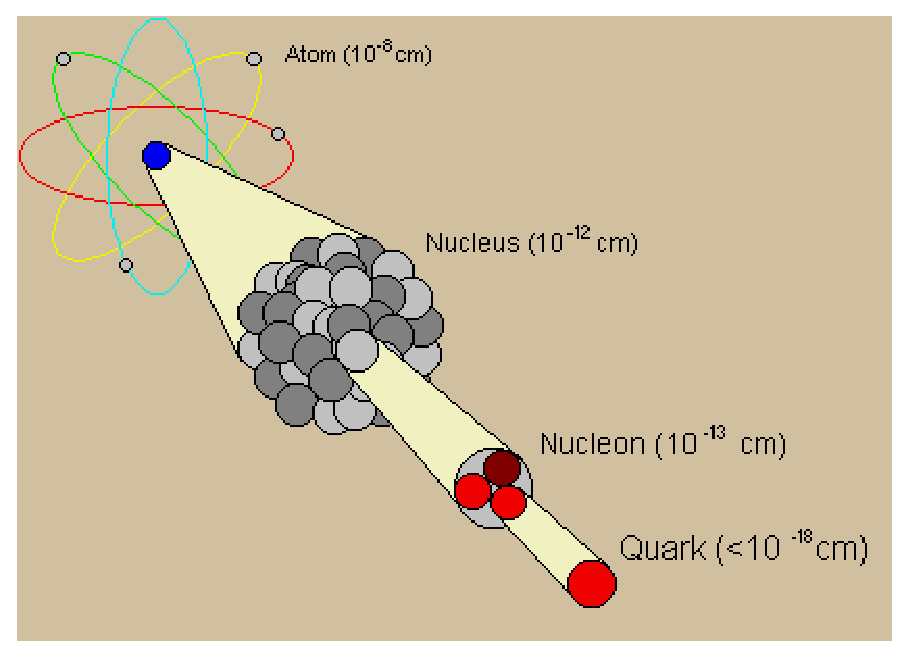
\includegraphics[type = eps, ext = .eps, scale = 1, bb = 0 0 420 300]{figs/atomo}
\end{slide}

\begin{slide}
\begin{center}
O Big-bang

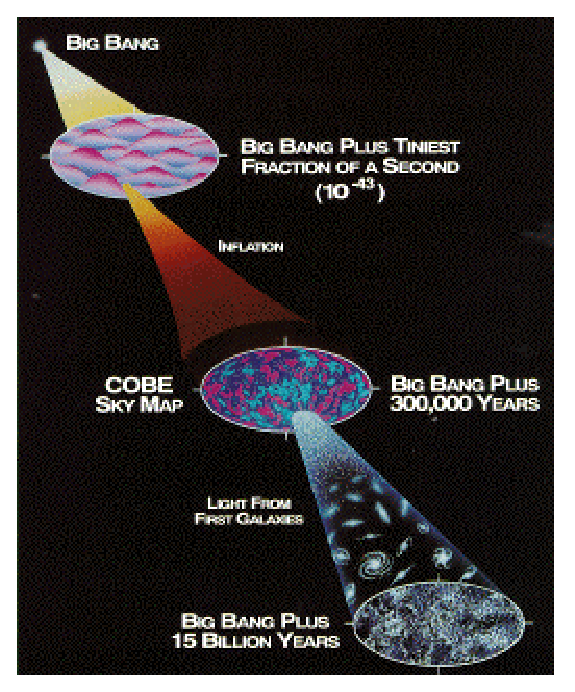
\includegraphics[type = eps, ext = .eps, scale = 1, bb = 0 0 260 316]{figs/bang}                

Os an�is aceleradores do CERN


\includegraphics[type = eps, ext = .eps, scale = 1, bb = 0 0 248 149]{figs/lhcair}
\end{center}
\end{slide}

\begin{slide}
O detetor ATLAS

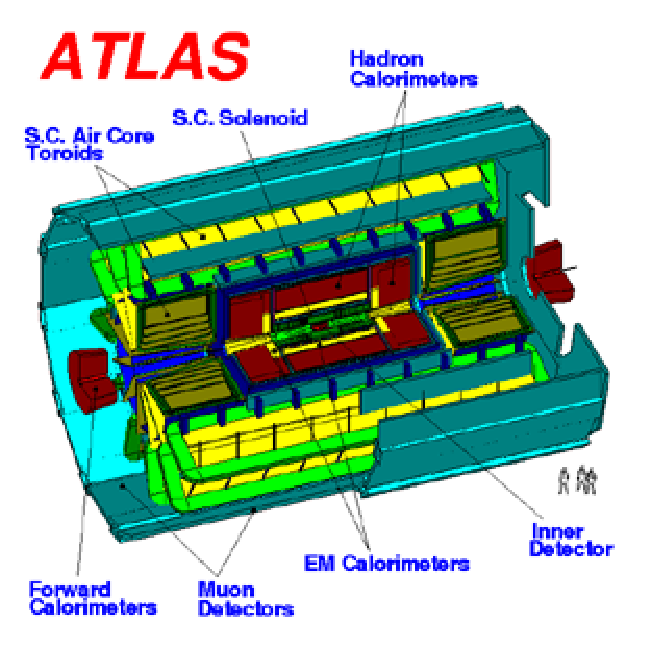
\includegraphics[type = eps, ext = .eps, scale = 1, bb = 0 0 300 295]{figs/atlasair}

Um evento reconstru�do

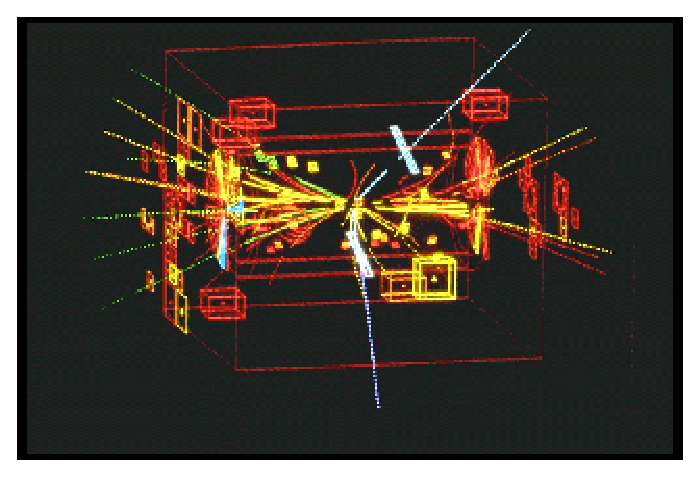
\includegraphics[type = eps, ext = .eps, scale = 1, bb = 0 0 320 213]{figs/colision}
\end{slide}

\begin{slide}
\begin{center}
Porque utilizar sistemas de valida��o ?

$\Downarrow$

Grande volume de dados

$\Downarrow$

\textcolor{blue}{\underline{Inviabilidade}} de armezenar tudo

$\Downarrow$

\textcolor{red}{\underline{Impossibilidade}} de faz�-lo
\end{center}
\end{slide}

\begin{slide}
O Sistema de \eng{Trigger} para o ATLAS

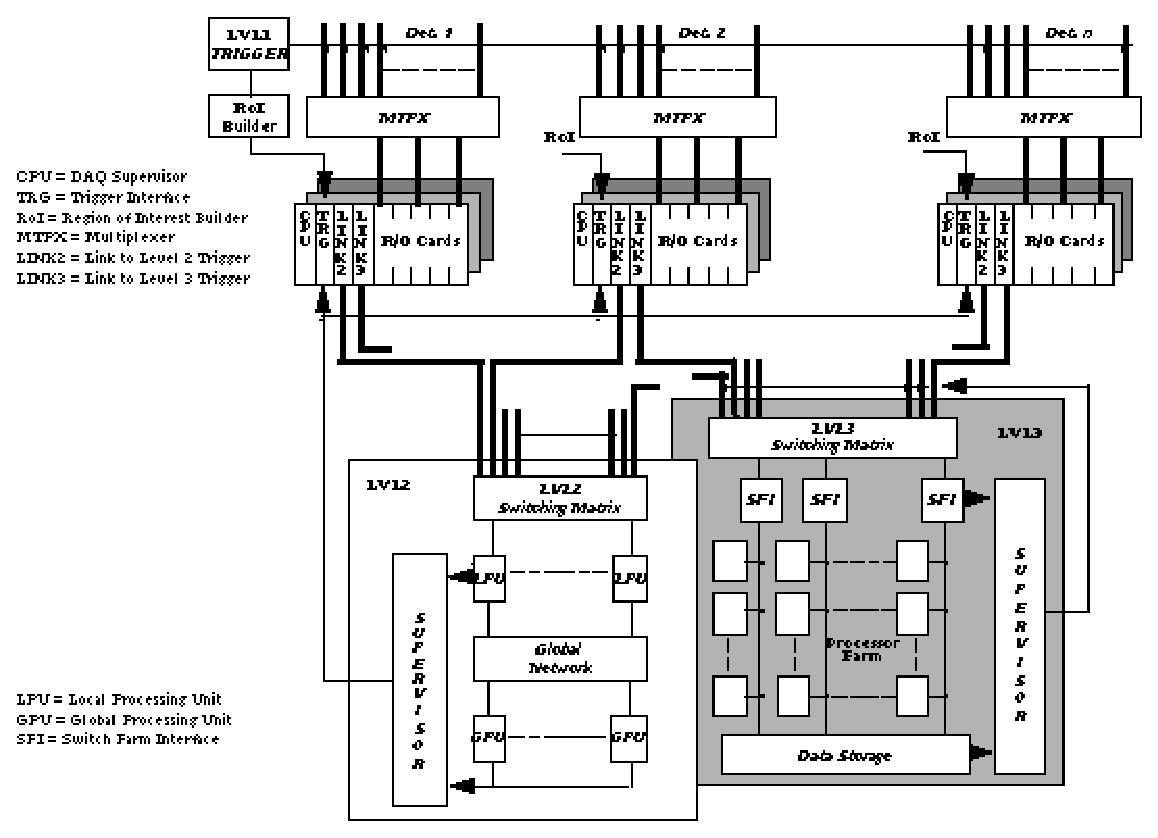
\includegraphics[type = eps, ext = .eps, scale = 0.8, bb = 0 0 540 386]{figs/trigger}
\end{slide}

\begin{slide}
Excitando os detetores

\input{picts/roi2.pic}
\end{slide}

\begin{slide}
A arquitetura A

{\tiny \input{picts/model_a2.pic}}
\end{slide}

\begin{slide}
A arquitetura B

{\tiny \input{picts/model_b2.pic}}
\end{slide}

\begin{slide}
A arquitetura C

{\tiny \input{picts/model_c2.pic}}
\end{slide}


 %% Whole introduction
\chapter{Revis�o da Literatura}
\label{chap:litera}
\index{Revis�o da Literatura}

Neste cap�tulo faremos a revis�o de algumas implementa��es e conceitos bem-sucedidos
 na descri��o e opera��o do 2\eiro n�vel de valida��o para o experimento ATLAS/LHC; 
destacam-se a utiliza��o de Redes Neurais como algor�tmo para alguns Extratores de 
Caracter�stica e unidades de Decis�o Global e, ainda, a utiliza��o de processamento 
paralelo em algumas implementa��es.

O motivo de tal direcionamento deste estudo deve-se � disponibilidade de 
equipamento com processamento distribu�do e bem-sucedidas implementa��es atrav�s de 
nosso grupo (Colabora��o Internacional CERN\-/\-COPPE\-/\-UFRJ) utilizando redes 
neurais artificiais na  
execu��o de extratores de caracter�sticas e unidades de decis�o global para a 
identifica��o de part�culas.

\section{Redes Neurais Artificiais e o processamento global para o segundo n�vel de
\eng{trigger}}
\index{Trigger!Level2!Redes Neurais aplicadas ao}
\index{Redes Neurais!Porque utiliz�-las no segundo n�vel de valida��o?}
\label{sec:ANN_at_globaldec}

Como elucidado na se��o~\ref{sec:level2}, o segundo n�vel de \eng{trigger} deve combinar as caracter�sticas 
vindas de diferentes subdetetores, de forma a aumentar a qualidade de classifica��o 
das part�culas. Neste est�gio � melhor n�o realizar uma identifica��o baseada em 
l�gica exclusiva, pois poderemos diminuir a qualidade de decis�o, mas gerar um outro 
conjunto de vari�veis, com probabilidades sobre a natureza da part�cula 
\cite{bock:ANN_at_level2}.

Considere o exemplo simples\index{Redes Neurais!Exemplo na classifi��o de 
part�culas} onde dois subdetetores n�o s�o correlacionados, ou 
seja, suas caracter�sticas extra�das s�o linearmente 
independentes (LI-s)\index{Independ�ncia Linear}. A forma mais ineficiente de 
fazer uma decis�o � a de classificar a part�cula segundo cada subdetetor e depois 
perfazer um ``E'' l�gico (AND) entre as classifica��es. Considere a ilustra��o 
da figura~\ref{fig:fexes} com as diferentes caracter�sticas extra�das da cada 
subdetetor (gen�rico), de tal forma que o n�vel de identifica��o para 2 tipos de 
excitadores de RoI, el�trons e jatos,  se d� com uma sobreposi��o de 10\%, o
 quer dizer que se tra�armos um corte para identifica��o em cada distribui��o 
teremos um erro m�nimo de 10\%. Neste exemplo a classifica��o exclusiva 
indicar� somente 81\% de corre��o na identifica��o das part�culas (o produto das 
probabilidades).

\begin{figure} 
 \begin{center}
 \caption{A distribui��o de caracter�sticas para cada subdetetor gen�rico. Os 
subsistemas s�o LI-s.} 
 \label{fig:fexes} 
 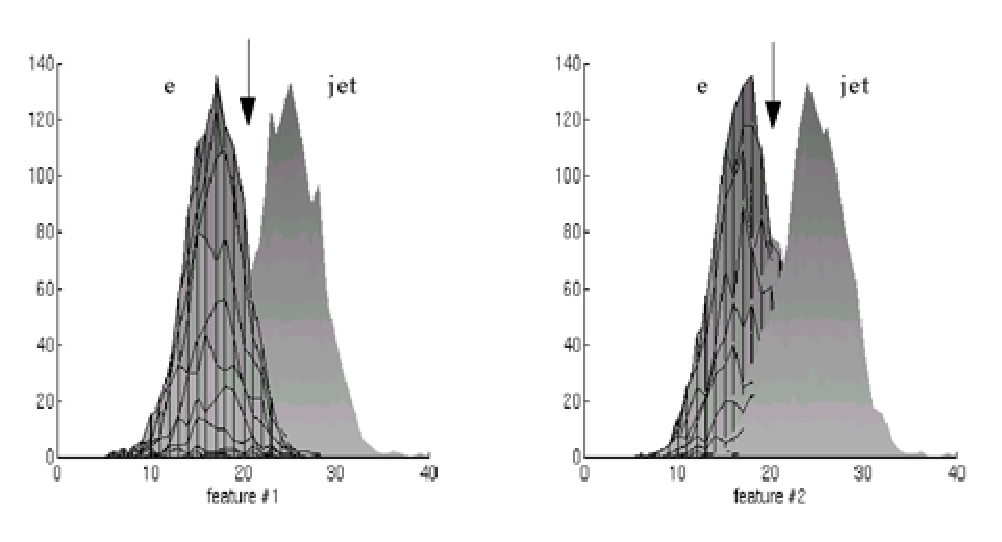
\includegraphics[type = eps, ext = .eps, scale = 0.9, bb = 0 0 464 243]{figs/fex_eg}
 \end{center}
\end{figure} 

A decis�o poder� ser melhor tomada se as duas caracter�sticas forem analisadas 
juntas, em um espa�o bidimensional (figura~\ref{fig:fex_bidim}). Cortando com um plano
como � mostrado, ambos os tipos de part�culas s�o 96\% corretamente classificadas. 
Estes tipos de cortes s�o realizados tamb�m por estruturas de Redes Neurais 
Artificiais utilizando a fun��o identidade como a fun��o de transfer�ncia para 
os neur�nios. Se o n�mero de subdetetores crescer, a diferen�a entre estas duas 
maneiras de classifica��o ficar� mais expl�cita, como � poss�vel observar na 
tabela~\ref{tab:efici_ann}. Neste teste foi considerado que todas as caracter�sticas 
foram extra�das de subsistemas LI-s, assim sendo, n�o houve necessidade da utiliza��o de
camadas escondidas.

\begin{figure} 
 \begin{center}
 \caption{Exemplo de classifica��o num espa�o bidimensional} 
 \label{fig:fex_bidim} 
 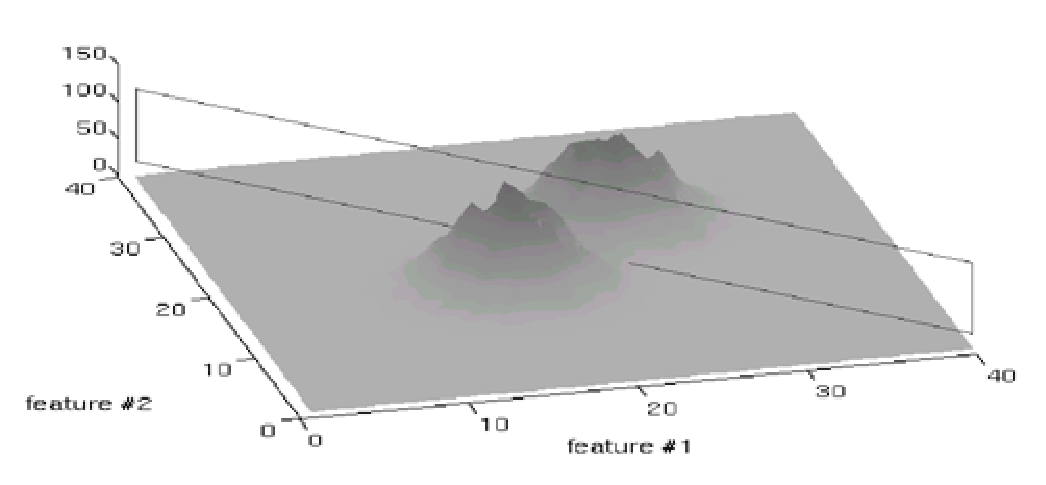
\includegraphics[type = eps, ext = .eps, scale = 0.85, bb = 0 0 485 216]{figs/fex_bid}
 \end{center}
\end{figure} 

\begin{table}
 \begin{center}
 \caption{Tabela de efici�ncias para uma classifica��o utilizando um ``E'' l�gico e 
Redes Neurais Artificiais simples, sem camadas escondidas.}
 \label{tab:efici_ann}
 \begin{tabular}{|c||c|c|}
 \hline
 N�mero de Detetores & Classifica��o com ``E'' l�gico & Classifica��o com ANN \\ 
 \hline \hline
 1 & 90\% & 90\% \\ \hline 
 2 & 81\% & 96.5\% \\ \hline 
 3 & 73\% & 98.8\% \\ \hline 
 4 & 65\% & 99.4\% \\ \hline 
 5 & 59\% & 99.8\% \\ \hline 
 \end{tabular}
 \end{center}
\end{table}\index{Redes Neurais!Tabela comparativa com se\-pa\-ra\-��o cl�s\-si\-ca}

Embora pare�a simples, a tarefa para a identifica��o de part�culas � um processo 
que envolve caracter�sticas extra�das dos dados de um n�mero de subdetetores menor 
que o n�mero de caracter�sticas\footnote{O n�mero de detetores est� entre 4 e 6 e o 
de caracter�sticas, entre 12 e 15.}, portanto, algumas destas s�o linearmente 
dependentes (LD-s)\index{Depend�ncia Linear}. Para m�xima efici�ncia na separa��o com vari�veis LD-s a 
utiliza��o de camadas escondidas � necess�ria. A figura~\ref{fig:LD_vars_and_ANNS} 
mostra o resultado de separa��o obtida sobre dados LD-s utilizando 3, 2 ou nenhum 
neur�nio na camada escondida.

\begin{figure} 
 \begin{center}
 \caption{Classifica��o em um espa�o de vari�veis linearmente dependente.} 
 \label{fig:LD_vars_and_ANNS} 
 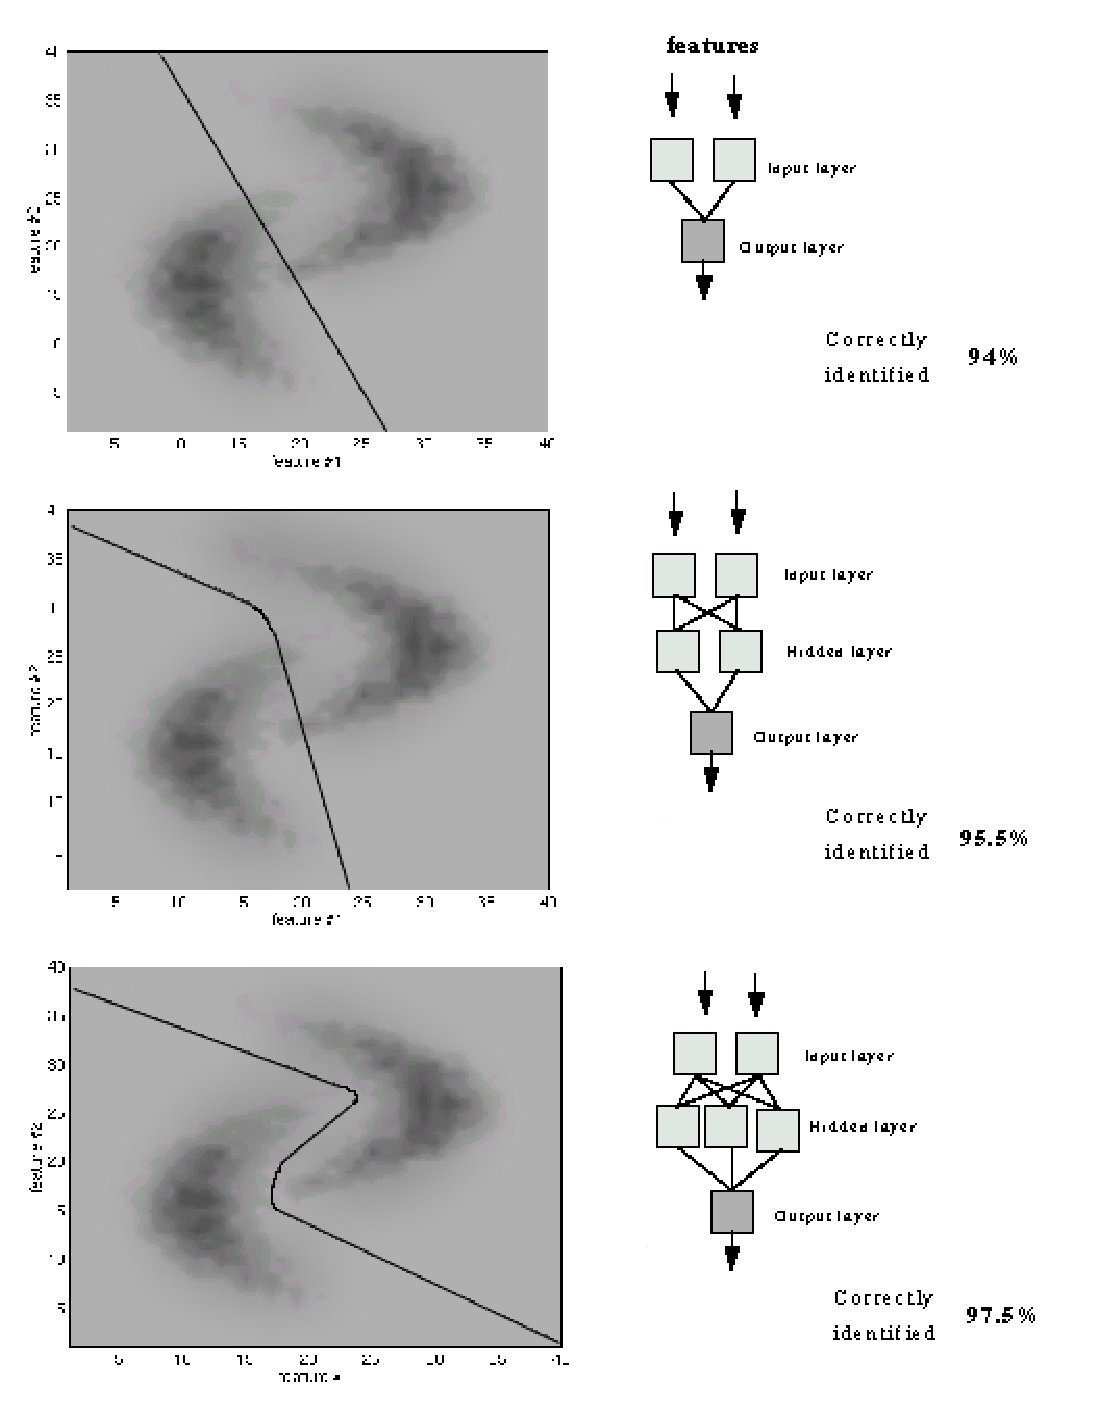
\includegraphics[type = eps, ext = .eps, scale = 0.8, bb = 0 0 511 661]{figs/annhid}
 \end{center}
\end{figure} 

\paragraph{Conclus�o:} O processamento de Decis�o Global ter� �tima efici�ncia se 
utilizarmos Redes Neurais Artificiais (ANN-s) ao inv�s de algoritmos basedos em 
classifica��o exclusiva, devido ao n�mero de subsistemas e vari�veis envolvidas. Em 
raz�o da depend�ncia entre as vari�veis dos diversos subsistemas parece inevit�vel 
a utiliza��o de ao menos uma camada escondida em uma rede neural simples, 
diretamente conectada (\eng{feed forward}).

Em particular, resultados com redes na configura��o 12-6-4, isto �, 12
entradas, 6 neur�nios na camada escondida e 4 na de sa�da t�m se mostrado satisfat�rios onde
tempo de processamento e efici�ncia s�o fatores dominantes como � poss�vel ver em 
\cite{sx:gldec}. O n�mero de sa�das � fortemente dependente da quantidade de 
part�culas diferentes que se deseja identificar no processamento da RoI. No 
caso espec�fico supracitado a identifica��o se fez por uma separa��o entre 4 
diferentes tipos de part�culas (el�trons, jatos, p�ons e m�ons).

Devemos destacar ainda que redes neurais s�o capazes de encontrar correla��es em 
espa�os multi-dimensionais ainda que na presen�a de grande quantidade de ru�do. 
Redes Neurais artificiais tamb�m podem ser muito competitivas onde pre�o e robustez 
s�o fatores delimitantes.

\section{A utiliza��o de ambientes de processamento distribu�do para o segundo n�vel de
 \eng{trigger}}
\index{Paralelismo!Porque utilizar?}

Devido �s altas taxas de eventos a que ser� submetido o segundo n�vel de 
\eng{trigger} (muitos Gigabytes por segundo e uma lat�ncia m�xima presumida de 1ms), a 
decomposi��o do problema atrav�s de paraleliza��o das atividades 
parece apontar um caminho para a solu��o. Esta
paraleliza��o pode ser implementada em 2 n�veis:
\begin{enumerate} 
 \item Na paraleliza��o de uma atividade simples como a extra��o de uma 
caracter�stica ou a identifica��o de uma part�cula, de modo a reduzir a lat�ncia do 
processamento localizado; e
 \item Na paraleliza��o de uma classe de atividades ou de todo o processamento para 
este n�vel, por exemplo, a extra��o de 
caracter�sticas utilizando uma \eng{farm} de processadores operando em paralelo 
sobre dados de diferentes RoI-s, reduzindo a lat�ncia do processamento como um todo e
 n�o localmente como no item anterior.
\end{enumerate}

Os dois tipos de paraleliza��o levam a diferentes enfoques de 
implementa��o\index{Paralelismo!enfoques}: no 
primeiro teremos um algoritmo baseado na taxa de dados (\eng{Data 
Driven})\index{Paralelismo!Data
Driven Approach}  de entradab visto que a 
paraleliza��o � feita de modo a reduzir as lat�ncias individuais, reduzindo  
a lat�ncia global do processo para cada evento. Nesta implementa��o deve-se utilizar  
uma arquitetura capaz de sustentar a taxa de dados, como em 
\cite{bock:cpp_at_level2}.

No segundo enfoque, a lat�ncia dos processos individuais n�o � demasiado importante, 
visto que poderemos compensar uma maior lat�ncia com a utiliza��o de mais 
processadores naquele n�vel de processamento. Este tipo de implementa��o � conhecido
 como \eng{Asynchronous Processor Farms 
Implementation}\index{Paralelismo!Asynchronous Approach} ou Implementa��o em 
\eng{farms} de processadores ass�ncronos. O assincronismo vem do fato das atividades
 paralelas serem independentes quanto ao tempo de execu��o entre si, podendo ser 
executadas totalmente livres do final (ou come�o) de processamento de qualquer evento
ou dado em qualquer outra unidade de processamento.

No caso do segundo n�vel em espec�fico\index{Paralelismo!Para o segundo n�vel}, 
podemos enxergar paralelismo em  
algumas das atividades realizadas e no processamento como um todo tamb�m. Para 
algoritmos de extra��o de caracter�sticas em calor�metros, t�cnicas de processamento 
paralelo  
ass�ncrono t�m se mostrado eficientes no atendimento das taxas de entrada do 
experimento, como � poss�vel ler em \cite{sx:fe}. 

Para as unidades de Decis�o Global, a utiliza��o de redes neurais artificiais t�m 
mostrado vantagem, como explicita a se��o~\ref{sec:ANN_at_globaldec}. Redes Neurais 
s�o algoritmos altamente paraleliz�veis por serem baseados em multiplica��es e somas 
vetoriais totalmente independentes ao n�vel de cada camada\footnote{� claro que os 
resultados da camada de ordem $n$ dependem dos resultados da camada de ordem 
$n-1$ e, sendo assim, n�o podemos tornar isto concorrente, ou seja, o processamento 
ainda deve ser feito camada a camada.}. Ainda, otimiza��es podem ser realizadas a 
n�vel ass�ncrono utilizando-se mais de uma rede para o processamento global.

Por fim, as atividades do segundo n�vel como um todo s�o paraleliz�veis visto a 
independ�ncia entre diferentes eventos. Estes podem ser processados 
independentemente (e, desta forma, ass�ncronamente) uns dos outros, sem perda 
de informa��es, de forma que a lat�ncia 
para cada evento possa ser aumentada proporcionalmente do valor alvo de 1ms para 
outro valor maior, dependendo de quantos forem os n�s de processamento adicionados. 
Este enfoque,  
� claro, reduz a necessidade de otimiza��o dos subn�veis de processamento internos 
ao segundo n�vel, como � o caso do enfoque baseado na taxa de dados (\eng{Data Driven 
Approach}).

\subsection{DSP-s}
\index{DSP-s!Utilidade}

\eng{Digital Signal Processors} (processadores digitais de sinais) n�o s�o mais do 
que r�pidos processadores matem�ticos que executam fun��es aritm�ticas b�sicas e 
outras fun��es complexas com poucos pulsos de \eng{clock}. Alguns DSP-s como o 
ADSP-21020 da Analog Devices podem processar em apenas 1 ciclo de \eng{clock} uma multiplica��o 
entre n�meros reais(ou pontos flutuantes).

Vantagens na utiliza��o de DSP-s s�o expl�citas quando o processamento depende do 
c�lculo de muitas vari�veis. No caso do processamento para o segundo 
n�vel, existem muitos subn�veis em que � poss�vel atingir uma redu��o da lat�ncia de
processamento utilizando-se DSP-s como processadores centrais do subn�vel \cite{bock:cpp_at_level2}.
Este � o caso da maioria dos extratores de caracter�stica e das unidades de decis�o 
global, se desenhados como Redes Neurais Artificiais.

\section{Arquiteturas para o segundo n�vel de \eng{trigger}}
\index{Trigger!Level2!Arquiteturas}

Limita��es de tamanho e custo podem nos levar a 3 poss�veis arquiteturas mutuamente 
exclusivas para o segundo n�vel de processamento\cite{level2:tsr}:
\begin{itemize} 
 \item{\bf Modelo A:} Utiliza uma parti��o local/global do segundo n�vel de processamento, 
com processamento at� a extra��o de caracter�sticas (inclusive) sendo realizado com 
arquitetura baseda no 
enfoque \eng{data-driven}, enquanto que o processamento global utiliza uma \eng{farm}
 de processadores utilizando o enfoque de processamento ass�ncrono;
 \item{\bf Modelo B:} Utiliza uma parti��o local/global de todo o processamento do 
segundo n�vel, fazendo uso de v�rias \eng{farms} feitas de processadores id�nticos ou
similares com extra��o de caracter�sticas paralela para cada subdetetor e para cada
RoI;
 \item{\bf Modelo C:} Uma �nica \eng{farm} de processadores realizando, cada um, o 
processamento relativo a um evento inteiro.
\end{itemize}

Estas arquiteturas seguem alguns crit�rios de funcionamento tais como n�o possuir 
lat�ncia de opera��o\footnote{Tempo de demora entre a decis�o do 1\eiro n�vel e a 
decis�o do segundo.} superior a 2 ms (modelo A) e 10 ms (modelos B e C); caso esta 
ultrapasse, o supervisor deve se responsabilizar por abortar a opera��o de valida��o 
para este evento. Estes crit�rios podem ser melhor estudados em 
\cite{level2:tsr} e \cite{level2:urd}.

\subsection{Modelo A}
\index{Trigger!Level2!Arquiteturas-Modelo A}

Neste modelo A, a informa��o de cada RoI � comunicada pelo \eng{RoI Builder} �s 
ROB-s (isto ainda � no 1\eiro n�vel). Os dados s�o ent�o ``empurrados'' atrav�s do 
pr�-processamento e cole��o de RoI-s para a extra��o de caracter�sticas. Nesta parte
de opera��o as unidades de processamento (acopladas, formando um �nico subsistema) 
dever�o suportar a mais alta taxa de eventos poss�vel. As opera��es s�o totalmente 
independentes para os dados de diferentes subdetetores. Para cada RoI, um vetor de 
dados � preparado contendo as caracter�sticas extra�das e um cabe�alho de 
identifica��o. Depois da extra��o de caracter�sticas, estes vetores s�o encaminhados
 a uma chave que � respons�vel por distribu�-los pelos processadores globais. A 
figura~\ref{fig:mod_a} pode ser elucidativa quanto ao mencionado nesta se��o.

\begin{figure} 
 \begin{center}
 \caption{Um diagrama esquem�tico para o modelo arquitetural A do segundo n�vel de 
valida��o.} 
 \label{fig:mod_a} 
 \input{picts/model_a.pic}
 \end{center}
\end{figure} 

\subsection{Modelo B}
\index{Trigger!Level2!Arquiteturas-Modelo B}

Neste modelo B, a informa��o de cada RoI � passada ao supervisor que controla {\bf 
todo} o fluxo de dados. Os dados de cada RoI s�o passados dos ROB-s atrav�s do 
pr�-processamento e cole��o de RoI-s a uma chave que se encarrega de passar os dados
 relativos a cada RoI para extratores de caracter�sticas. Nesta fase, os subsistemas
 relativos a cada subdetetor s�o totalmente independentes, podendo ter seus pr�prios
 supervisores locais. As caracter�sticas 
extra�das s�o, ent�o, passadas atrav�s de outra chave (que re�ne as caracter�sticas 
extra�das de cada subdetetor sobre uma mesma RoI), que repassa estes dados �s 
unidades de decis�o global. A figura~\ref{fig:mod_b} mostra um diagrama ilustrativo.

\begin{figure} 
 \begin{center}
 \caption{Um diagrama esquem�tico para o modelo arquitetural B do segundo n�vel de 
valida��o.} 
 \label{fig:mod_b} 
 \input{picts/model_b.pic}
 \end{center}
\end{figure} 

\subsection{Modelo C}
\index{Trigger!Level2!Arquiteturas-Modelo C}

Neste modelo C, a informa��o � passada a um supervisor central que dedica um dos 
processadores de uma \eng{farm} homog�nea a todo o processamento do evento. Este 
processador controla todo o fluxo de dados da RoI pelos ROB-s e pelas unidades de 
pr�-processamento e cole��o de RoI-s. Os dados, depois de coletados, seguem a uma 
chave que os repassa ao devido processador de evento, para que este realize a extra��o
 de caracter�sticas e a decis�o global. A figura~\ref{fig:mod_c} mostra um diagrama 
ilustrativo.

\begin{figure} 
 \begin{center}
 \caption{Um diagrama esquem�tico para o modelo arquitetural C do segundo n�vel de 
valida��o.} 
 \label{fig:mod_c} 
 \input{picts/model_c.pic}
 \end{center}
\end{figure} 

\section{Concluindo alguns pontos...}
\index{Revis�o da Literatura!conclus�o}

� poss�vel utilizar ANN-s para desenhar alguns subsistemas do segundo n�vel de 
valida��o, em especial Unidades de Decis�o Global e Extratores de Caracter�sticas 
para Calor�metros. Estas redes especializadas no reconhecimento de padr�es podem ter sua 
lat�ncia reduzida se utilizarmos computa��o distribu�da uma vez que seu algoritmo � 
altamente paraleliz�vel. Ainda, se utilizarmos DSP-s como processadores centrais de 
alguns destes subsistemas poderemos nos beneficiar de sua alta performance 
computacional em algoritmos envolvendo repetidos c�lculos.

A paraleliza��o da aplica��o (ainda que complexa) poder� acontecer em 2 inst�ncias: 
na primeira,  
local, h� uma paraleliza��o buscando a otimiza��o de um algoritmo utilizado em 
um subsistema, de forma a atender �s taxas de entrada e lat�ncia m�ximas deste 
subsistema; chamamos este enfoque de \eng{data-driven} uma vez que os dados fluir�o 
por estes subsistemas sem restri��es ou controle, j� que estes suportar�o as taxas de 
entrada m�ximas. Na segunda inst�ncia, global, acontece uma paraleliza��o de subsistemas 
id�nticos (exemplo: Extratores de Caracter�stica) de forma que a lat�ncia m�xima para
cada evento seja aumentada proporcionalmente ao n�mero de processadores 
anexados. Em particular a paraleliza��o em primeira inst�ncia n�o ser� aqui 
utilizada visto que equipamento espec�fico para cada subsistema paraleliz�vel � 
requerido. Utilizaremos, no entanto, o conceito de paraleliza��o global, 
ou em segunda inst�ncia como veremos mais a frente.

Existem v�rios modelos para a implementa��o do segundo n�vel, cada um com suas 
vantagens e desvantagens, embora de uma forma geral bem plaus�veis. Para fins 
e objetivos deste projeto, no entanto, nos concentraremos no modelo B. O modelo A 
requer utiliza��o de processamento  
diversificado para a camada de pr�-processamento, cole��o de RoI-s e Extra��o de 
Caracter�sticas, o que n�o ser� poss�vel, pois somente dispomos de 16 processadores em 
nossa m�quina (v�-la-emos em detalhes mais adiante) que ter�o seus potenciais 
subaproveitados se os utilizarmos em uma paraleliza��o local ou em primeira 
inst�ncia.

O modelo C exige um chaveamento a partir dos ROB-s utilizando uma chave muito r�pida
(tecnologia ATM), que tamb�m n�o se encontra em nosso poder. A arquitetura B, no 
entanto, nos  
parece mais adpt�vel ao equipamento dispon�vel (TELMAT TN310) e que queremos 
avaliar; sendo assim, 
tentaremos abordar o problema e construir o simulador baseado neste desenho. 
Lembramos que queremos atingir 2 metas aqui: a primeira � construir um 
sistema de valida��o, a segunda, testar a tecnologia contida em uma TN310 de 
forma a avaliar globalmente arquitetura e equipamento para a realiza��o do segundo 
n�vel de valida��o para o experimento ATLAS\-/\-LHC.
 
No que se segue exporemos em detalhes alguns dos conceitos, materiais e m�todos 
utilizados neste projeto, isto �, Redes Neurais Artificiais, a m�quina 
mencionada - Telmat TN310, os dados utilizados e alguns conceitos de paralelismo.

 %% Documentation Revision
%% This file contains 6 slides
\begin{slide}
Redes Neurais Artificiais - O neur�nio artificial

\begin{center}
{\tiny \input{picts/neuronc.pic}}
\end{center}
RNA multi-camadas

\begin{center}
{\tiny \input{picts/multi.pic}}
\end{center}
\end{slide}

\begin{slide}
O Sistema TN310

\begin{itemize} 
 \item Processamento Distribu�do
 \item 16 n�s independentes
 \item Mem�ria Local (MIMD)
 \item HTRAM-s tamanho 4
 \begin{enumerate} 
  \item T9000
  \item ADSP 21020 (196Kbytes)
  \item 8Mbytes RAM
  \item 256Kbytes \eng{shared}
 \end{enumerate}
 \item Totalmente conectado atrav�s de chaves STC104
\end{itemize}
\end{slide}

\begin{slide}
O T9000

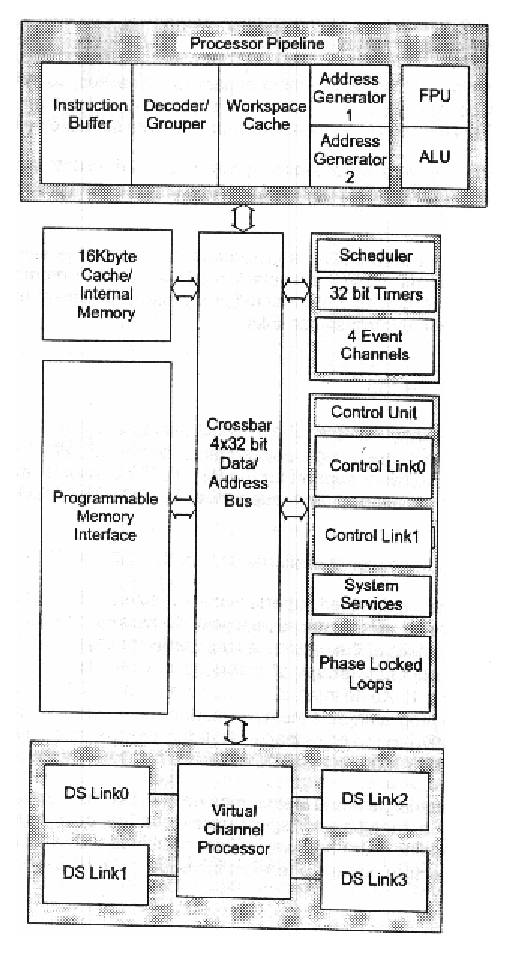
\includegraphics[type=eps, ext=.eps, bb= 0 0 228 441]{figs/T9000}
\end{slide}

\begin{slide}
O ADSP 21020

\end{slide}

\begin{slide}
A conex�o entre os n�s na TN310

{\tiny \input{picts/connect2.pic}}
\end{slide}

\begin{slide}
N�veis de programa��o

\begin{center}
{\tiny \input{picts/layer.pic}}
\end{center}

Comunica��o por canais
\begin{center}
{\tiny \input{picts/chan_op2.pic}}
\end{center}
\end{slide}


 %% Theoretical Fundaments, Methods and Materials used at this project
%% This file contains 9 slides
\begin{slide}
Modelo de neur�nio utilizado

\begin{center}
{\tiny \input{picts/neuronc.pic}}
\end{center}

A rede para a GDU
\begin{center}
{\tiny \input{picts/gdu_net.pic}}
\end{center}
\end{slide}

\begin{slide}
\begin{center}
Tabela de convers�o

{\tiny \input{picts/lut_ex2.pic}}

GDU em paralelo

{\tiny \input{picts/gdu_full.pic}}
\end{center}
\end{slide}

\begin{slide}
A comunica��o com os escravos

{\tiny \input{picts/shake.pic}}

O supervisor (fluxograma)
z
\begin{center}
{\tiny \input{picts/sup_flow.pic}}
\end{center}
\end{slide}

\begin{slide}
{\small
Resultados para a GDU
\begin{itemize} 
 \item O tempo de processamento para uma RoI da GDU rodando em apenas 1 n� � de 200$\mu$s
 \item Alocando o supervisor no n� zero e 15 escravos o tempo de processamento por 
RoI � de 30,3$\mu$s (\eng{speed-up} = 6.6)
 \item Alocando o supervisor no n� 15 e 15 escravos o tempo de processamento cai 
para 27$\mu$s (\eng{speed-up} = 7.4)
\end{itemize}
Conclus�es
\begin{itemize} 
 \item Tabela de convers�o � eficiente - reduzimos o tempo de processamento sem 
perder efici�ncia
 \item A aloca��o ``inteligente'' de tarefas leva a melhores resultados
 \item \eng{speed-up} - Bom desempenho, mas � o m�ximo ? 
\end{itemize}}
\end{slide}

\begin{slide}
� implementar no 2\eiro n�vel

{\tiny \input{picts/mod_bi2.pic}}
\end{slide}

\begin{slide}
Generaliza��o

\begin{center}
{\tiny \input{picts/top_tn.pic}}
\end{center}
\end{slide}

\begin{slide}
\label{slide:implementa}
Implementa��o usando os 16 n�s

{\tiny \input{picts/sim_v2a2.pic}}
\end{slide}

\begin{slide}
Resultados para a vers�o em apenas 1 n�
\begin{itemize} 
 \item N�o leva em considera��o tempo de distribui��o (necess�rio)
 \item Tempo para uma RoI = 1320$\mu$s
\end{itemize}
Resultado para a vers�o concorrente 1 (aloca��o aleat�ria)

$\Rightarrow$ Tempo para uma RoI = 830$\mu$s (\eng{speed-up} = 1,6)

Resultado para a vers�o concorrente 2 (aloca��o ``inteligente'')

$\Rightarrow$ Tempo para uma RoI = 690$\mu$s (\eng{speed-up} = 1,9)

Resultados para a vers�o concorrente 3 (distribui��o sequencial)

$\Rightarrow$ Tempo para uma RoI = 390$\mu$s (\eng{speed-up} = {\bf 3,4 !})
\end{slide}

\begin{slide}
Conclus�es
\begin{itemize} 
 \item Sabendo que \eng{speed-up} m�ximo � 4 ($//$ dados e fluxo) atingimos 85\% do 
m�ximo
 \item Melhora de 43\% da vers�o 3 para a vers�o 2
 \item Considerando 1 e\-ven\-to $\approx$ 5 RoI-s $\Rightarrow$ 2ms\-/\-e\-ven\-to (500Hz)
 \item Lentid�o $\Rightarrow$ Tempo de distribui��o dos dados para fex-s $\Rightarrow$ 96\% do 
tempo total de aplica��o
 \item Atingimos o m�ximo desta tecnologia ?
\end{itemize}
\end{slide}

 %% Project implementation and constraints at TN310
\chapter{Resultados obtidos e Conclus�es}
\label{chap:results}

Neste cap�tulo, estaremos expondo os resultados obtidos com as implementa��es expostas
no cap�tulo anterior. Para todas as implementa��es, consideramos o \eng{speed-up} em 
rela��o a uma vers�o simples da aplica��o, isto �, rodando em um �nico processador. 
Tamb�m � feita uma revis�o dos tempos de comunica��o e afins.

Inicialmente, repassaremos testes realizados sobre o tempo de comunica��o do sistema 
TN310. Estes testes visaram a um entendimento operacional do tempo de processamento 
dispendido durante comunica��es entre aplica��es. Na segunda se��o, traremos 
resultados para a aplica��o do sistema de decis�o global e na se��o seguinte, 
exporemos os resultados e conclus�es para a simula��o do sistema de valida��o.

\section{Teste de comunica��es}
\secl{time}

Em equipamentos com n�mero de n�s de processamento consider�vel � necess�rio o 
entendimento pleno do sistema de comunica��o utilizado. Quando menciona-se 
``Entendimento Pleno" quer se acentuar que para uma otimiza��o das rotinas h�
 a necessidade de o programador desenvolver uma ``afinidade'' muito grande com o 
equipamento. Esta afinidade traduz-se no entendimento de todos os detalhes de 
funcionamento do sistema, sejam eles de alto ou de baixo n�vel.

O processo de comunica��o entre os diversos n�s de processamento no sistema TN310 
n�o � diferente,  
isto �, ele possui uma interface de alto n�vel (como as fun��es da 
tabela~\tabr{channel.h}) e uma interface de baixo n�vel, inerente ao sistema. A 
interface de alto n�vel � respons�vel pelo processo de comunica��o em si, mas os 
motivos pelos quais alguns tipos de comunica��o s�o diferentes de outros � um ponto 
que somente pode ser explicado com o entendimento do sistema operando em baixo 
n�vel. Desta forma, antes de entrarmos nos resultados destes testes propriamente,
abordaremos alguns aspectos na forma de comunica��o entre os diversos n�s HTRAM do 
sistema TN310.

\subsection{Introdu��o ao sistema de comunica��es}

O sistema de comunica��es da TN310 � totalmente baseado no conceito de chaveamento 
ass�ncrono de pacotes (\eng{Asynchronous Packet Switch}). Este tipo de sistema pode 
aumentar a ``performance'' em ambientes maiores, como � caso. Ele se baseia na utiliza��o
 de uma chave r�pida (STC104) para que haja a distribui��o de pacotes pela rede de 
forma mais r�pida e livre de erros poss�vel. Estas chaves podem rotear at� 32 
pacotes diferentes ao mesmo tempo, vindo de quaisquer 32 localidades distintas e 
indo para outras 32 localidades tamb�m distintas.

A id�ia �, na verdade, bem simples. Quando uma informa��o deseja ser mandada de um 
ponto a outro, a tarefa no ponto emissor envia uma mensagem ao processador virtual de
 canais local indicando o endere�o e o tamanho do dado a ser mandado. O processador 
de canais divide o dado a ser enviado em v�rios pacotes de tamanho predeterminado. 
Ap�s esta divis�o, a cada pacote � adicionado um cabe�alho contendo a loca��o-destino 
e a rota para o pacote. O pacote � enviado a uma chave que interpreta a primeira parte do 
cabe�alho e envia o pacote para o n� correto, removendo a parte do cabe�alho 
referente � rota j� informada e deixando exposta a parte do cabe�alho referente ao 
n�-destino do pacote. Ao chegar ao n�-destino,
cada pacote � autenticado (i.e., verifica-se se realmente se est� esperando 
tal informa��o e se o cabe�alho est� correto) e um reconhecimento (\eng{acknowledgement}) 
� enviado para que o pr�ximo pacote seja mandado, se este for o caso.

No caso de o pacote ter que passar por 2 chaves, 3 cabe�alhos s�o inseridos a cada 
pacote. Este ser� roteado atrav�s de 2 chaves e ocorrer�o 2 remo��es de 
cabe�alhos (\eng{header deletion}) e apenas um ser� utilizado novamente no n� destino.
Desta forma, � poss�vel garantir que poderemos criar um n�mero muito grande de 
canais virtuais. Comunica��o utilizando canais virtuais nada mais � do que 
comunica��o feita com pacotes de dados  intercalados simulando um sistema com maior 
n�mero de conex�es do que realmente existem.

Quando � dito que h� uma multiplexa��o dos canais, quer-se dizer que, uma
vez que s�o dividos em pacotes, os dados a serem enviados podem ser intercalados, 
gerando uma rede de multiplexa��o de pacotes e, assim, satisfazendo um grande n�mero 
de canais simult�neos, chamados virtuais. 

A figura~\figr{header_del} pode ser elucidativa quanto � remo��o de cabe�alhos.

\begin{figure} 
 \begin{center}
 \caption{O processo de dele��o de cabe�alho em uma rede com chaveamento ass�ncrono 
de pacotes.} 
 \figl{header_del} 
 \input{picts/head_del.pic}
 \end{center}
\end{figure} 

\paragraph{Concluindo.} A TN310 � um sistema distribu�do com 16 n�s de processamento
tipo HTRAM totalmente conectados atrav�s de uma rede de chaves ass�ncronas. A 
comunica��o nesta rede � feita atrav�s canais descritos em \eng{software} (InMOS C), mas
implementados via \eng{hardware} atrav�s de um sistema de canais virtuais cujo 
processador central � o VCP (Processador de Canais Virtuais). O VCP divide a 
informa��o a ser mandada em pacotes e a cada pacote adiciona um n�mero de cabe�alhos
proporcional ao n�mero de n�s por onde o pacote passar�. Assim sendo, se o pacote 
tiver que passar por 2 chaves adicionar-se-�o 3 cabe�alhos (2 para as chaves e 1 para 
o n�-destino). Os pacotes s�o enviados intercaladamente com outros pacotes de outras
informa��es que tamb�m est�o sendo enviadas. Isto cria uma rede de canais virtuais.

\subsection{Os testes}

Levando em considera��o que estaremos alocando em cada n� de processamento uma �nica
tarefa seq�encial, isto �, sem que dispare processos concorrentes, podemos chegar � 
conclus�o que todos os DS-Links estar�o � disposi��o da aplica��o para a transmiss�o
de dados. Isto maximiza a utiliza��o dos meios de comunica��o de cada n�. Estamos 
interessados em entender 2 pontos na opera��o do sistema:
\begin{enumerate} 
 \item Qual � o tamanho de cada pacote mandado por vez?
 \item Quanto tempo demora para que pacotes sejam enviados a diferentes n�s de 
processamento?
\end{enumerate}
   
A primeira quest�o tem um motivo pr�tico: sabendo o tamanho do pacote, 
podemos maximizar seu uso. A segunda quest�o se refere ao tempo gasto para que 
enviemos uma quantidade fixa de dados de um ponto para outro do sistema. Ao saber 
isto, estaremos aptos a tomar melhores decis�es sobre a aloca��o de processos e 
avaliar melhor o quadro de opera��o de uma aplica��o.

O teste realizado consiste em mandar dados de diferentes tamanhos para 
diferentes n�s de processamento e medir o tempo gasto durante esta transfer�ncia. 
Saberemos que este tempo representa a melhor condi��o poss�vel de opera��o, onde os 4
DS-Links estar�o � disposi��o do processo de comunica��o. O envio de dados ocorreu 
de forma iterativa, embora tenhamos descontado o tempo de itera��o no final do 
processo. A itera��o serviu para que pud�ssemos avaliar mais precisamente o tempo de
comunica��o para os diversos tamanhos de dados.

Os resultados encontram-se na tabela~\tabr{time}. A tabela exp�e na horizontal o 
tempo (em $\mu$segundos) para que haja a transmiss�o do n�mero de bytes indicados � 
direita atrav�s de 4 tipos diferentes de conex�o. Cada tipo representa o n�mero de 
chaves existentes entre os n�s de processamento. Existem diferentes tipos de 
conex�es, como foi visto na se��o~\secr{connect}. A conex�o do tipo 1 representa a
 conex�o entre dois n�s onde ocorre apenas uma chave; a do tipo 2, 2 chaves e, 
assim, sucessivamente, at� 4 chaves (conex�o entre os n�s 0 e 8).

\begin{table}
 \caption[Os tempos gastos para os diversos tamanhos de dados comunicados a 
diferentes n�s de processamento.]{Os tempos gastos para os diversos tamanhos de dados 
comunicados a diferentes n�s de processamento. Tempos em microssegundos e tamanho em 
bytes ou pacotes de 32 bytes.} 
 \tabl{time}
 \begin{center}
  \begin{tabular}{|r|r|c|c|c|c|} \hline
Tamanho (bytes)& Tamanho (pacotes) & Tipo 1 & Tipo 2 & Tipo 3 & Tipo 4 \\ \hline \hline
1 at� 32 & 1 & 10,2 & 12,1 & 13,8 & 15,5 \\ \hline
33 at� 64 & 2 & 16,9 & 20,6 & 24,0 & 27,6\\ \hline
65 at� 96 & 3 & 23,5 & 28,9 & 34,2 & 39,5\\ \hline
100 & 4 & 30,2 & 37,5 & 44,6 & 51,8 \\ \hline
150 & 5 & 37,2 & 46,0 & 54,7 & 63,6 \\ \hline
200 & 7 & 50,5 & 62,9 & 75,3 & 87,6 \\ \hline
250 & 8 & 57,2 & 71,4 & 85,4 & 99,5 \\ \hline
300 & 10 & 70,8 & 88,2 & 106 & 123 \\ \hline
350 & 11 & 77,3 & 96,7 & 116 & 136 \\ \hline
400 & 13 & 90,6 & 114 & 136 & 159 \\ \hline
450 & 15 & 104 & 130 & 157 & 183 \\ \hline
500 & 16 & 111 & 139 & 167 & 195 \\ \hline
550 & 18 & 124 & 156 & 188 & 219 \\ \hline
600 & 19 & 131 & 164 & 198 & 231 \\ \hline
650 & 21 & 114 & 181 & 218 & 255 \\ \hline
700 & 22 & 151 & 190 & 228 & 261 \\ \hline
750 & 24 & 164 & 206 & 249 & 291 \\ \hline
800 & 25 & 171 & 215 & 255 & 303 \\ \hline
850 & 27 & 184 & 232 & 219 & 327 \\ \hline
900 & 29 & 197 & 245 & 300 & 351 \\ \hline
950 & 30 & 204 & 257 & 310 & 363 \\ \hline
1000 & 32 & 217 & 274 & 331 & 387 \\ \hline
1500 & 47 & 317 & 400 & 484 & 567 \\ \hline
2000 & 63 & 424 & 535 & 647 & 758 \\ \hline
2500 & 79 & 531 & 670 & 810 & 950 \\ \hline
3000 & 94 & 631 & 797 & 964 & 1130 \\ \hline
3500 & 110 & 737 & 931 & 1130 & 1320 \\ \hline
4000 & 125 & 838 & 1060 & 1280 & 1500 \\ \hline
4500 & 141 & 944 & 1190 & 1440 & 1690 \\ \hline
5000 & 157 & 1050 & 1330 & 1610 & 1880 \\ \hline
5500 & 172 & 1150 & 1450 & 1760 & 2060 \\ \hline
6000 & 188 & 1260 & 1590 & 1920 & 2260 \\ \hline
6500 & 204 & 1360 & 1720 & 2090 & 2450 \\ \hline
7000 & 219 & 1460 & 1850 & 2240 & 2630 \\ \hline
7500 & 235 & 1570 & 1990 & 2400 & 2820 \\ \hline
8000 & 250 & 1670 & 2110 & 2560 & 3000 \\ \hline
8500 & 266 & 1790 & 2250 & 2720 & 3190 \\ \hline
9000 & 282 & 1900 & 2400 & 2880 & 3380 \\ \hline
9500 & 297 & 2000 & 2530 & 3040 & 3560 \\ \hline
10000 & 313 & 2120 & 2670 & 3200 & 3760 \\ \hline
  \end{tabular}
 \end{center}
\end{table}

Com este resultado, percebemos que o tamanho do pacote mencionado anteriormente � de 
32 bytes. Este valor � fixo para comunica��es em qualquer dist�ncia. Isto quer dizer
que a inclus�o de mais ou menos cabe�alhos n�o influencia no tamanho do pacote 
enviado. 

A aplica��o foi feita de forma que as tarefas escravas receptoras de dados 
sempre estariam dispon�veis para o recebimento de dados, nunca atrasando a 
tarefa-mestra. Um fator interessante � que podemos perceber que, em verdade, o que ocorre  
� uma distribui��o de pacotes. Este fato fica marcante se olharmos a 
segunda parte da tabela, que indica ``tamanho (em pacotes)''. Ao compararmos o envio 
de 1 pacote, logo utilizando 1 dos 4 DS-Links dispon�veis, o tempo de demora � um. 
Por�m, se estivermos mandando mais de um pacote, logo utilizando mais de um DS-Link,
 o tempo por pacote cai, ainda que o tempo total aumente. Isto se deve ao fato de 
que o VCP processa os dados a serem enviados seq�encialmente, o que obrigatoriamente
 nos leva a um aumento do tempo, mas vemos que o simples fato de enviar 2 pacotes 
quase simultaneamente reduz o tempo total cerca de 16\% (essa taxa reduz quanto 
maior o n�mero de chaves na conex�o chegando at� 11\%). Se enviarmos 3 pacotes a taxa 
de redu��o chega a 23\%, para 4, a 26\% e assim segue at� que esta taxa atinja o 
valor de 34\%,  
quando enviamos mais de 300 pacotes utilizando os 4 DS-Links. Esta taxa pode ser 
mencionada como taxa de satura��o, i.e., representa o m�ximo na otimiza��o de 
comunica��o ating�vel (para conex�es do tipo 1) usando 4 canais simult�neos, ao inv�s 
de apenas 1. 

Estes resultados mostram que o envio de mais de 4 pacotes nesta situa��o (uma tarefa 
por processador) parece ser uma caracter�stica interessante em termos de otimiza��o.
Os processos podem ser ajustados para que o volume de comunica��es n�o seja menor do
que 4 pacotes por vez. Pelo fato da rede estar totalmente conectada atrav�s de chaves 
ass�ncronas e os DS-Links terem cada um uma conex�o com a rede, se usarmos 
a configura��o de uma tarefa (sem processos concorrentes) por processador, nunca 
teremos congestionamento de dados. 

Depois do entendimento do processo de comunica��o e troca de dados, veremos as 
implementa��es propostas no cap�tulo~\ref{chap:project}.

\section{Resultados para a GDU}

\subsection{Replicando o JETNET}
\secl{gdu_single}

Implementamos 2 processos distintos para a unidade de decis�es globais; no primeiro 
tentamos replicar os resultados obtidos com o pacote JETNET no ambiente do sistema 
TN310 (InMOS C), usando os pesos, \eng{thresholds} e vetores de normaliza��o achados 
durante a fase de treinamento neste primeiro ambiente (JETNET). A 
tabela~\tabr{eficience_ic} mostra os resultados de efici�ncia obtidos  
utilizando o programa do ap�ndice~\ref{ap:global1}. Quando mencionamos efici�ncia de
uma RNA queremos destacar sua capacidade no reconhecimento de padr�es, assim, uma 
efici�ncia de 90\% significa que de cada 100 part�culas de um dado tipo a rede 
consegue \textbf{corretamente} identificar 90 e, assim, sucessivamente.

\begin{table}
 \caption[As efici�ncias para a rede 12-6-4 da GDU usando InMOS C.]{As efici�ncias 
para a rede 12-6-4 da GDU usando InMOS C. Os valores para $\pi^{-}$ n�o foram 
computados por n�o representarem um volume de dados expressivo. As marcas ``---'' 
indicam que n�o aconteceram part�culas daquele tipo no arquivo de entrada.}
 \tabl{eficience_ic}
 \begin{center}
  \begin{tabular}{|c|c|c|c|c|} \hline
             & $4e^{-}$ & $2e^{-}+2j$ & $2e^{-}+2\mu$ & $4\mu$ \\ \hline \hline
  $e^{-}$ & 97.45 & 99.50 & 94.75 & ---\\ \hline
  $jets$ & 93.40 & 96.13 & 96.40 & 100\\ \hline
  $\mu$ & --- & 94.44 & 100 & 99.95\\ \hline
  \end{tabular}
 \end{center}
\end{table}

O tempo de processamento m�dio por RoI foi de 200 microssegundos. Este tempo leva
em considera��o somente o processamento neuronal da RoI; a leitura e escrita em 
disco foram realizadas sem contar tempo de processamento. O casamento perfeito entre
a tabela~\tabr{eficience} e a tabela~\tabr{eficience_ic} mostra a validade da 
substitui��o do c�lculo utilizando s�ries (\raw{tanh()}) por uma tabela de convers�o. 
Esta substitui��o tamb�m reduz o tempo de processamento requerido por RoI.

\subsection{A GDU concorrente}

A segunda vers�o do programa, operando em 15 n�s no sistema TN310; foi executada em 2
configura��es: na primeira alocamos os processos como descrito na 
tabela~\tabr{aloc_v1}.

\begin{table}
 \caption{A GDU concorrente, vers�o 1 - Mapa de aloca��o de processos.}
 \tabl{aloc_v1}
 \begin{center}
  \begin{tabular}{|c|c|} \hline
  Tarefa & Processador \\ \hline \hline
  Supervisor & 0 \\ \hline
  15 GDU-s & 1 ao 15 \\ \hline
  \end{tabular}
 \end{center}
\end{table}

Optamos por esta configura��o para demostrarmos que diferentes posicionamentos dos 
processos podem nos levar a resultados bem diferentes. O tempo de processamento 
encontrado para uma ROI foi, aproximadamente, de 30,3 microssegundos. Consideramos o 
fator de   
agiliza��o da aplica��o (\eng{speed-up}) como a rela��o entre o tempo gasto para 
processar 1 RoI na aplica��o constru�da em apenas um n� do sistema TN310 e o tempo 
gasto para processar 1 RoI em qualquer outra configura��o da mesma aplica��o 
operando em mais de um n� de processamento do sistema. Neste caso, o \eng{speed-up} da 
aplica��o, quando a comparamos com a vers�o que roda em apenas 1 n� de processamento
este resultado de 30,3 $\mu s$ por RoI, fica em torno de 6,6.

Se utilizarmos a organiza��o apontada na tabela~\tabr{aloc_v2}, o tempo de 
processamento por evento cai para cerca de 27 microssegundos por RoI. Isto nos leva 
a um \eng{speed-up} de 7,4.

\begin{table}
 \caption{A GDU concorrente, vers�o 2 - Mapa de aloca��o de processos.}
 \tabl{aloc_v2}
 \begin{center}
  \begin{tabular}{|c|c|} \hline
  Tarefa & Processador \\ \hline \hline
  Supervisor & 15 \\ \hline
  15 GDU-s & 0 ao 14 \\ \hline
  \end{tabular}
 \end{center}
\end{table}

\subsection{Conclus�es sobre a unidade de decis�es globais}

Os dados recolhidos aqui, sem contar com as efici�ncias, representam a m�dia 
aritm�tica de milhares de itera��es. Isto significa que estes dados est�o t�o 
pr�ximos dos valores m�dios quanto foi poss�vel chegar. De forma nenhuma os valores 
aqui apresentados representam dados esp�rios ou ocasionais.

\paragraph{A tabela de convers�o.} A utiliza��o da tabela de convers�o provou-se 
muito eficiente como forma de substitui��o da aritm�tica complexa envolvida no 
c�lculo de fun��es como a tangente hiperb�lica. Neste caso espec�fico, a substitui��o
da fun��o implementada por expans�o em s�rie por uma tabela de convers�o mostrou-se
ideal, visto que consiguimos diminuir o tempo de processamento sem termos reduzido a 
efici�ncia de separa��o da rede.

\paragraph{O tempo de processamento em 1 n�.} O tempo de processamento por RoI em 1 
n� encontrado (200 $\mu s$) � representativo do processamento neural da RoI, n�o 
incluindo de forma alguma as rotinas de leitura e escrita dos dados de cada RoI. O 
processamento neuronal, neste caso espec�fico, consiste de 86 somat�rios, 72 
multiplica��es e 10 ativa��es. Sabendo que 1 ciclo de um processador dura no m�nimo 
1 microssegundo\footnote{Embora o \eng{clock} seja de 20MHz (50ns por pulso) cada ciclo do 
\eng{transputer} � executado em 1 microssegundo para processos em alta prioridade e em 
64ms para processos em baixa prioridade.} e que realizamos 168 opera��es distintas,
sendo que 10 delas s�o mais complexas (ativa��o da \raw{NET} dos neur�nios) dir�amos 
que o valor de 200$\mu s$ por RoI � bem satisfat�rio e coerente.

\paragraph{Aloca��o de tarefas.} Uma diferen�a de at� 10\% no tempo de processamento
 pode ser observado se realocarmos de forma eficiente os processos. Este fator 
exemplifica que o bom programador � aquele que conhece o equipamento com que 
trabalha, pois desta forma consegue aproveitar o m�ximo de cada recurso.

\paragraph{O \eng{Speed-up}.} O valor para o \eng{speed-up} de 7,4 � um bom 
resultado. O valor m�ximo para esta caracter�stica �, no caso espec�fico de 15 
escravos concorrentes, 15. Uma vez que o tempo gasto na comunica��o introduz uma 
seq�encializa��o na aplica��o, como visto na se��o \secr{data_par}, � de se esperar 
que este fator de agiliza��o se reduza drasticamente. 

De uma forma geral, a aplica��o de v�rias t�cnicas como o paralelismo de dados, a 
convers�o de valores por tabelas e a otimiza��o baseada na organiza��o de 
\eng{hardware} conseguiram multiplicar em at� 7,4 vezes a velocidade de execu��o de 
uma rede neuronal. A utiliza��o de uma m�quina de processamento distribu�do neste 
caso mostrou-se eficaz.

\section{Resultados para a implementa��o do segundo n�vel de \eng{trigger}}

Apresentaremos aqui os resultados obtidos com as 3 vers�es de implementa��o para o 
segundo n�vel de valida��o do experimento ATLAS/LHC. Destacamos aqui, como fizemos 
anteriormente, que atingimos a m�xima otimiza��o atrav�s de v�rias implementa��es 
como se seguem. 

\subsection{Resultados para o algoritmo completo rodando em apenas 1 processador}

Foi simulado o processamento completo de uma RoI, 100 vezes (para tirarmos uma 
m�dia), utilizando-se de apenas um n� de processamento. Este processamento consiste 
em, sequencialmente, extrair-se as caracter�sticas da RoI e pass�-la na rede neural 
12-6-4 das unidades de decis�o global. O tempo de processamento para cada RoI foi de 
1,7 ms em m�dia. Este processamento n�o inclui, � claro, a parte relativa �s Redes 
Locais, que s� t�m sentido de implementa��o em sistemas distribu�dos. Isto se deve 
ao fato de que Redes Locais representam processos de distribui��o e recolhimento de 
dados, o que n�o ocorre em uma vers�o seq�encial da aplica��o, pois n�o h� 
distribui��o dos dados por um sistema complexo. Os dados mant�m-se em uma �nica 
unidade de processamento por todo o tempo.

Os tempos simulados para os algoritmos de extratores estavam de acordo com os dados
da tabela~\tabr{fexor_proc}.

O valor de 1,7 ms ser� utilizado para calcularmos o \eng{speed-up} das aplica��es 
que se seguem. Utilizaremos o mesmo crit�rio de c�lculo utilizado na avalia��o da 
agiliza��o para a unidade de decis�es globais: dividiremos o tempo de processamento 
de uma RoI processada por apenas um n� pelo tempo gasto para processar uma RoI em 
configura��es que utilizem mais de um n� de processamento, como as que se seguem; 
assim, chegaremos ao que consideramos o \eng{speed-up} da aplica��o.

\subsection{Resultados para a vers�o 1}

Ao executarmos esta vers�o chegamos aos resultados contidos na 
tabela~\tabr{simul_1_results}.
 
\begin{table}
 \caption{Os resultados obtidos com a implementa��o da primeira vers�o do simulador 
para o sistema de valida��o. Totais para 500 RoI-s.}
 \tabl{simul_1_results}
 \begin{center}
  \begin{tabular}{|c|c|c|} \hline
  & Tempo ($ms$) & \% do tempo total \\ \hline \hline
  Distribui��o de dados para Extratores & 365.079 & 87,93 \\ \hline
  Perda com verifica��es redundantes & 29.580 & 7,12 \\ \hline
  Total de aplica��o & 415.189 & 100 \\ \hline
  \end{tabular}
 \end{center}
\end{table}

Podemos perceber que o maior ``gargalo'' de nossa aplica��o encontra-se na distribui��o 
de dados para os extratores de caracter�stica, somando aproximandamente 90\% do 
tempo total da aplica��o. Embora existam t�cnicas para otimizar a comunica��o entre 
tarefas, n�o h� como eliminarmos por completo ou em boa parte o tempo gasto nesta 
distribui��o. Isto se deve a fatores puramente l�gicos: a passagem de dados da 
aplica��o supervisora para os extratores de caracter�stica � necess�ria, ou n�o 
teremos aplica��o. Outro fator interessante a ser lembrado � que jamais 
conseguiremos otimizar o fluxo de dados nesta aplica��o, pois todos os canais com 
extratores de caracter�stica demandam um alto volume de dados, portanto j� 
utilizando mais de um DS-Link por vez.

O tempo de processamento para cada RoI fica em torno de 830 $\mu s$.
O \eng{speed-up} �:
\begin{displaymath}
speed-up = \frac{1700}{830} = 2,05,
\end{displaymath}
que � um valor baixo.
Tentamos a otimiza��o por realoca��o dos processos como se segue.

\subsection{Resultados para a vers�o 2}

Ao realocarmos os processos de uma forma mais eficiente, esperamos que os tempos 
gastos em comunica��o se reduzam; desta forma ter�amos um aumento do \eng{speed-up} 
da aplica��o. Os resultados est�o na tabela~\tabr{simul_2_results}. Tentamos, 
tamb�m, eliminar o tempo gasto com a verifica��o de extratores cujos os dados j� 
acabaram, tentando minimizar o tempo de processamento.

\begin{table}
 \caption{Os resultados obtidos com a implementa��o da segunda vers�o do simulador 
para o sistema de valida��o. Totais para 500 RoI-s.}
 \tabl{simul_2_results}
 \begin{center}
  \begin{tabular}{|c|c|c|} \hline
  & Tempo ($ms$) & \% do tempo total \\ \hline \hline
  Distribui��o de dados para Extratores & 335.695 & 97,58 \\ \hline
  Perda com verifica��es redundantes & 0 & 0 \\ \hline
  Total de aplica��o & 344.015 & 100 \\ \hline
  \end{tabular}
 \end{center}
\end{table}

O tempo gasto com a verifica��o de extratores parados foi totalmente retirado, ainda 
que tenhamos sofrido alguma penalidade na redu��o das dist�ncias entre os processos, 
a medida que tivemos que adicionar c�digo para a elimina��o deste tempo extra.

O tempo de processamento para cada RoI baixou para 688 $\mu s$. Isto significa que o 
\eng{speed-up} aumentou, vejamos:
\begin{displaymath}
speed-up = \frac{1700}{688} = 2,47.
\end{displaymath}

Embora estejamos pr�ximos de um aumento de 20\%, estes ajustes ainda n�o 
caracterizariam uma boa ``performance'' pelo equipamento. Visto que uma abordagem 
tentando maximizar a utiliza��o dos canais n�o aponta bons resultados, pois o �nico 
canal a ser otimizado � para a distribui��o de dados para extratores de m�ons, que 
n�o se encontram t�o distantes da otimiza��o m�xima, direcionamo-nos para a implementa��o 
utilizando a distribui��o circular de eventos, como abordado na 
se��o~\secr{simul_v3}.

\subsection{Resultados para a vers�o 3}

Esta vers�o tira proveito da sequencializa��o do processo de distribui��o de eventos
e de rotinas especiais, otimizadas para a utiliza��o na implementa��o em alto n�vel
de canais virtuais criados em \eng{hardware}, caso espec�fico do Transputer T9000.
Este conjunto de rotinas � conhecido como \raw{DirectChan-s}, e funciona de forma 
id�ntica �s rotinas da tabela~\tabr{channel.h}, apenas de forma mais r�pida.

Os resultados desta vers�o de implementa��o encontram-se na 
tabela~\tabr{simul_3_results}.
\begin{table}
 \caption{Os resultados obtidos com a implementa��o da terceira vers�o do simulador 
para o sistema de valida��o. Totais para 500 RoI-s.}
 \tabl{simul_3_results}
 \begin{center}
  \begin{tabular}{|c|c|c|} \hline
  & Tempo ($ms$) & \% do tempo total \\ \hline \hline
  Distribui��o de dados para Extratores & 194.427 & 96 \\ \hline
  Perda com verifica��es redundantes & 0 & 0 \\ \hline
  Total de aplica��o & 203.453 & 100 \\ \hline
  \end{tabular}
 \end{center}
\end{table}

O tempo para o processamento de uma RoI atinge, nesta implementa��o, cerca de 
390 $\mu s$.
O \eng{speed-up}:
\begin{displaymath}
speed-up = \frac{1700}{390} = 4,36.
\end{displaymath}

\subsection{Concluindo sobre o sistema de valida��o}

Cabe aqui uma pequena revis�o do processo de paraleliza��o como um todo; para isto 
repetiremos aqui algumas das figuras mostrando o processo de modelagem e implementa��o
da aplica��o. 

Inicialmente est�vamos diante de uma apl�ca��o de dif�cil paraleliza��o, mostrada 
na figura~\figr{mod_b_implementation} e repetida aqui na 
figura~\figr{conclusion_1}. Esta aplica��o possui 2 n�veis de paraleliza��o 
distintos, um segundo o seu fluxo, pois atua como um \eng{pipeline} processando os 
dados no sentido dos extratores para as unidades de decis�o global; e outro segundo seus 
dados. Neste caso estaremos atuando sobre um volume de dados cuja natureza e 
grandeza s�o as mesmas; poderemos, ent�o, utilizar processamento repetido para que 
agilizemos o processo como um todo.

\begin{figure} 
 \begin{center}
 \caption{O diagrama da aplica��o implementada no sistema TN310.} 
 \figl{conclusion_1} 
 \input{picts/mod_b_i.pic}
 \end{center}
\end{figure} 

A aplica��o destas duas t�cnicas neste �ltimo diagrama (figura~\figr{conclusion_1}) 
nos leva ao diagrama de tarefas da figura~\figr{conclusion_2}. Este diagrama foi 
arranjado de forma a maximizar a utiliza��o dos processadores e minimizar as cargas
sobre cada n� de processamento, balanceando o sistema.
                                                              
\begin{figure} 
 \begin{center}
 \caption{As tarefas da aplica��o.} 
 \figl{conclusion_2} 
 \input{picts/simul1.pic}
 \end{center}
\end{figure} 

O \eng{speed-up} para tal aplica��o vir�, portanto, na forma de 2 caracter�sticas 
adicionadas � execu��o do sistema, sua paraleliza��o de dados e sua paraleliza��o de
fluxo. Se somente pud�ssemos observar o paralelismo de dados, o \eng{speed-up} 
m�ximo a ser encontrado estaria entre 2 e 3, pois possu�mos apenas 2 unidades 
concorrentes  
para extratores de calor�metro e m�ons, ainda que tenhamos operando 3 unidades de 
processamento para extratores de TRT e 3 para SCT.

Por�m, a exist�ncia de um paralelismo de fluxo nos leva a um acr�scimo substancial no
\eng{speed-up} m�ximo ating�vel. Este acr�scimo � diretamente proporcional ao n�mero de 
subprocessos do \eng{pipeline} que est�o sendo executados paralelamente. Neste caso 
temos 2 subprocessos paralelos, a extra��o de caracter�sticas e a decis�o global, 
levando-nos a um \eng{speed-up} m�ximo entre 4 e 6. Isto pode ser visualizado com um 
simples exemplo:

\begin{quotation}
Imaginemos uma linha de montagem para autom�veis. Um autom�vel demora um tempo $x$ 
para ser constru�do. Por�m se tivermos $y$ trabalhadores especilizados na montagem 
de partes exclusivas do autom�vel, de forma que consigam terminar todo um ve�culo sem
ajuda de mais trabalhadores, estes conseguir�o imprimir uma velocidade maior no 
processamento de ve�culos. No caso idealizado, quando a linha de montagem j� se 
encontra operacional (as diversas partes j� possuem trabalho a ser feito) teremos a 
produ��o de $y$ ve�culos no mesmo tempo $x$.
\end{quotation}

De forma mais gen�rica, se utilizarmos paralelismo de fluxo em uma aplica��o que 
processa infinitamente, o \eng{speed-up}, quando o n�mero de produtos finais 
aumenta, tender� ao n�mero de subtarefas que s�o executadas simultaneamente. Assim, 
se 2 passos forem fluxo-paralelizados, o \eng{speed-up} ser�, quando o n�mero de 
dados processados for grande o suficiente, 2. Para 3 passos paralelizados, o 
\eng{speed-up} passa para 3 e, assim, sucessivamente.

O resultado obtido para o \eng{speed-up} em nossa aplica��o foi de aproximadamente 
4,4. Este resultado exprime quase 100\% do \eng{speed-up} m�ximo da aplica��o, 
\underline{na configura��o exposta}. Seria de valor reduzido tentarmos reprojet�-la de 
forma a aumentarmos o \eng{speed-up} m�ximo ating�vel\footnote{Isto seria poss�vel 
se realoc�ssemos 2 das 3 unidades de decis�o global para trabalharem como os 
extratores ausentes para os subsistemas de calor�metro e m�on.}, pois o tempo gasto 
com a distribui��o de dados atinge, na m�xima otimiza��o, enormes 96\% do tempo 
total de aplica��o. Isto reflete que o rearranjo jamais se traduziria em aumento do
\eng{speed-up} final de forma significativa, podendo at� reduz�-lo por estarmos 
desbalanceando o peso em cima das subtarefas de nossa aplicaca��o (deixando apenas 
uma unidade de decis�o global operando, sem aplicarmos paralelismo de dados).

\subsubsection{O sistema para o processamento de segundo n�vel}

Por outro lado, o resultado obtido utilizando-se apenas 1 n� de processamento nos 
mostra que, talvez, para uma aplica��o que n�o esta, fosse mais vi�vel a utiliza��o 
de muitos processadores operando sobre todo uma RoI (extra��o de caracter�stica e 
decis�o global) do que a distribui��o do processo por v�rias subtarefas. No entanto,
isto feriria a configura��o proposta para a arquitetura B (n�o fact�vel, segundo 
\cite{level2:tsr}) do segundo n�vel de 
valida��o. De fato, este esquema estaria mais adaptado � arquitetura C para o 
segundo n�vel, cuja implementa��o atrav�s de nosso equipamento seja invi�vel, 
pois requeriria a utiliza��o de chaves muito r�pidas (ATM), que n�o se encontram 
dispon�veis.

O fato de n�o possuirmos n�s em n�mero grande o suficiente para 
que consigamos suportar a taxa de fluxo do segundo n�vel de valida��o (100MHz), �, 
possivelmente a causa deste resultado. O tempo de processamento para uma RoI beira 
os 390 microssegundos; sabendo que o n�mero de RoI-s por evento �, na m�dia, de 5, isto
nos d� um tempo de processamento de cerca de 2 ms por evento, que � um valor 
baixo. Baixo porque n�o estamos considerando aqui duas importantes etapas do 
processamento de um evento, o preprocessamento que consta da transforma��o da RoI 
geom�trica disparada pelo n�vel 1 na RoI real, como explanado na se��o~\secr{preproc}
 e a decis�o sobre o canal f�sico do evento, parte integrante da tarefa de decis�es 
globais. Levando isto em considera��o, os 2 ms, ainda assim, representam 
a inexpressiva taxa de 500 Hz, baix�ssima para suportar a opera��o do segundo n�vel 
de \eng{trigger}.

\subsubsection{M�ximos e m�nimos}
\secl{max_min}

Ao construirmos a aplica��o para a unidade de processamento global percebemos que, 
ainda que utilizando distribui��o circular (\eng{Round-Robin}), atingimos um 
\eng{speed-up} de 7,4 utilizando a configura��o da figura~\figr{gdu_full}. O 
\eng{speed-up} m�ximo previsto, no entanto, era de 15, pois est�vamos lidando com 15
escravos.

A quest�o �: ``Porque o m�ximo que consiguimos foi 7,4?''. A resposta � um tanto 
complexa e nos basearemos nos resultados da tabela~\tabr{time} para que a 
respondamos.

A distribui��o circular provou-se �til pois, sempre que ating�amos o �ltimo escravo,
o primeiro j� estava livre; assim, jamais precisar�amos questionar a ocupa��o de um 
dado escravo j� que saber�amos de ante-m�o que ele estaria apto a receber novos 
dados e repassar os dados antigos j� processados, se a distrui��o mantivesse a ordem
(circular) inicial. Com este conhecimento � poss�vel formular esta pergunta: ``Qual � 
o n�mero \underline{m�nimo} de escravos que necessito para que o primeiro 
\textbf{sempre} esteja livre quando o supervisor passar dados para o �ltimo?''. A 
resposta desta pergunta pode nos levar a 2 novos caminho de implementa��o:

\begin{enumerate} 
 \item{\bf Reduzir o n�mero de escravos:} Assim ser� se o n�mero de 
processos-escravos necess�rios para mantermos fluxo de dados ininterrupto no 
supervisor for menor do que o que estamos utilizando (15). Isto significa que mais 
de um escravo est� ``parado'' quando dados s�o distribu�dos para o �ltimo.
 \item{\bf Emular mais escravos:} Assim ser� se o n�mero de escravos necess�rios 
para manter o fluxo de dados constante e ininterrupto no supervisor for maior que o 
que temos agora (15).
\end{enumerate}

Caso a resposta seja a primeira, deveremos provar que isto � verdade reduzindo o 
n�mero de escravos ao n�mero projetado e verificando se n�o h� degrada��o da 
``performance'' do sistema. Neste caso, mediremos isto pelo \eng{speed-up} da 
aplica��o, se este reduzir, 
 notaremos que houve preju�zo na redu��o do n�mero de escravos indicando 
necessidade de maior n�mero destes processos. Caso n�o reduza comprovaremos que este
 desenvolvimento � coerente e que estamos atingindo o \underline{m�ximo} desta 
aplica��o \underline{na configura��o proposta}.

Caso a resposta seja a segunda, deveremos implementar um sistema de emula��o. 
Durante uma emula��o acontece uma esp�cie de \textit{ensaio} onde simular-se-� o 
n�mero de n�s-de-processamento que ser�o suficientes para que atinjamos um fluxo de 
dados ininterrupto na aplica��o supervisora. Assim, se chegarmos, por exemplo, que 
o n�mero de escravos necess�rio � 30 devemos alocar em cada n� de processamento uma 
unidade de decis�o global que recebe 2 RoI-s, mas que, na realidade, gasta o tempo de 
processamento de uma �nica regi�o ``emulando'' a exist�ncia de mais 
n�s-de-processamento, neste caso 2.

Uma unidade de decis�o global, segundo a se��o~\secr{gdu_single}, demora 200 $\mu s$
para processar uma RoI. A passagem de dados de/para escravos, como pode ser 
visto na aplica��o descrita no ap�ndice~\ref{ap:sup_global}, acontece quando a 
aplica��o supervisora recolhe os dados processados anteriormente pelo escravo e 
repassa novos dados para serem processados. Numa situa��o onde existam somente 
conex�es do tipo 1 (isto �, com uma chave apenas ligando os processos supervisor
 e escravo) o tempo gasto nesta atividade ser� de, no m�nimo, 27 microssegundos. 
Este n�mero vem do seguinte c�lculo: cada unidade de decis�o global consome 12 
n�meros em ponto flutuante (reais); isto consome 48 bytes, que, segundo a 
se��o~\secr{time}, deve ser divido em 2 pacotes que demorar�o (em uma conex�o do 
tipo 1) cerca de 17 $\mu s$ para que sejam entregues. J� os dados processados s�o em
n�mero de 4 (reais) e consomem 16 bytes que podem ser enviados � aplica��o 
supervisor por atrav�s de um �nico pacote que leva cerca de 10 $\mu s$ para que seja
recebido (talvez um pouco mais). Esta troca de dados consumir�, ent�o, os 27 $\mu s$
mencionados.

Levando estes dados em considera��o necessitaremos de
\begin{displaymath}
\frac{200 \mu s}{27 \mu s} \approx 7,4 (\Longrightarrow 8)
\end{displaymath}
escravos. Isto quer dizer que, se tivermos 8 escravos para distribuirmos dados 
\textbf{depois} de distribuirmos dados para o primeiro escravo, este, e somente este, 
estar� livre  
quando acabarmos de distribuirmos dados para o �ltimo escravo. Seguindo a l�gica, o 
segundo processo escravo, e somente este, estar� livre quando acabarmos de 
distribuir dados para o primeiro e, assim, sucessivamente.

Isto est� de acordo com a primeira assun��o que fizemos alguns par�grafos 
acima no texto: o n�mero de escravos � menor que 15, isto significa que n�o 
precisaremos emular uma vers�o da unidade de decis�o global concorrente. Devemos 
ent�o, a partir do esquema da figura~\figr{gdu_full} ir eliminado o n�mero de 
escravos e verificar quando temos degrada��o de performance do sistema. De fato, 
como � poss�vel ver na tabela~\tabr{max_glob} a ``performance'' do sistema n�o cai 
at� que usemos menos de 9 escravos na GDU concorrente, re-afirmando a validade dos 
dados da tabela~\tabr{time} e das assun��es de funcionamento do sistema expostas 
anteriormente.

\begin{table}
 \caption{Os resultados para a GDU concorrente quando reduzimos o n�mero de 
processos escravos.}
 \tabl{max_glob}
 \begin{center}
  \begin{tabular}{|r|c|c|} \hline
 N�mero de escravos & Tempo para 1 RoI & \eng{speed-up} \\ \hline \hline
 15 & 27 $\mu s$ & 7,4 \\ \hline
 10 & 27 $\mu s$ & 7,4 \\ \hline
{\bf  9} & {\bf 27 $\mu s$} & {\bf 7,4} \\ \hline
{\bf  8} & {\bf 28,5 $\mu s$} & {\bf 7,0} \\ \hline
  7 & 32,5 $\mu s$ & 6,2 \\ \hline
  5 & 44,6 $\mu s$ & 4,5 \\ \hline
  3 & 74,2 $\mu s$ & 2,7 \\ \hline
  \end{tabular}
 \end{center}
\end{table}

Outra importante observa��o � que o valor calculado (7,4) �, exatamente, o 
\eng{speed-up} m�ximo para esta configura��o e, ao mesmo tempo, o n�mero de escravos
(menos 1) necess�rios para que o supervisor mantenha-se sempre distribuindo dados.

� poss�vel levantarmos as mesmas quest�es para o segundo n�vel de valida��o: ``Ser� 
que estamos usando processadores demais?''. Esta quest�o deve ser respondida da 
mesma forma que respondemos a quest�o similar para a GDU. Aqui, por�m, deveremos nos
 concentrar na parte de distribui��o de dados que mais pesa ao funcionamento do 
sistema como um todo, que � a distribui��o de dados para os extratores de 
caracter�stica. 

Esta distribui��o acontece, diferentemente da que acontece na GDU concorrente, 
somente no sentido do supervisor para as unidades de extra��o e leva tempos 
distintos para diferentes sistemas de extra��o. A tabela~\tabr{time:ext} pode ser 
elucidativa quanto aos tempos gastos em conex�es do tipo 1 para a passagem de dados 
do supervisor para os extratores. J� a tabela~\tabr{time_proc:ext} mostra os tempos 
de processamento de cada unidade.

\begin{table}
 \caption{Tempos gastos na passagem de dados da aplica��o supervisora para os 
extratores.}
 \tabl{time:ext}
 \begin{center}
  \begin{tabular}{|l|c|c|c|} \hline
Tipo de extrator & Tamanho (em bytes) & Tamanho (em pacotes) & Tempo \\ \hline 
\hline
Calor�metro & 504 & 16 (15,75) & 111 $\mu s$ \\ \hline
TRT & 420 & 14 (13,13) & 98 $\mu s$ \\ \hline
SCT & 420 & 14 (13,13) & 98 $\mu s$ \\ \hline
M�on & 60 & 2 (1,88) & 17 $\mu s$ \\ \hline
  \end{tabular}
 \end{center}
\end{table}

\begin{table}
 \caption{O tempo gasto em processamento dos dados em cada tipo de extrator de 
caracter�stica.}
 \tabl{time_proc:ext}
 \begin{center}
  \begin{tabular}{|c|c|} \hline
  Tipo de extrator & Tempo \\ \hline \hline
  Calor�metro & $10\mu s$ \\ \hline
  TRT & $400\mu s$ \\ \hline
  SCT (PreShower) & $250\mu s$ \\ \hline
  M�on & $5\mu s$ \\ \hline
 \end{tabular}
 \end{center}
\end{table}

Para que seja poss�vel atender o maior dos tempos de processamento (desta forma 
estaremos atendendo tamb�m os menores), neste caso o do extrator para o TRT (400 
$\mu s$, deveremos ter tempos de comunica��o com outros extratores quaisquer 
(inclusive com outros extratores para TRT), o mais pr�ximo poss�vel, ainda que maior,
 de 400 $\mu s$. Para que isto se concretize, \textbf{qualquer} configura��o que 
atenda este crit�rio poder� ser a configura��o m�nima para sistema. 

Assim podemos pensar em v�rias destas configura��es como se seguem:
\begin{enumerate} 
 \item {\bf 1 Ext.TRT, 2 Ext.SCT, 2 Ext.Calor�metro e 1 Ext.M�on};
 \item {\bf 1 Ext.TRT, 3 Ext.SCT, 1 Ext.Calor�metro e 1 Ext.M�on};
 \item {\bf 2 Ext.TRT, 1 Ext.SCT, 2 Ext.Calor�metro e 1 Ext.M�on};
 \item {\bf 2 Ext.TRT, 1 Ext.SCT, 1 Ext.Calor�metro e 6 Ext.M�on}
 \item etc 
\end{enumerate}

Se o leitor somar os tempos de comunica��o, ver� que esta soma � mais que suficiente para
cobrir quaisquer dos tempos de processamento. Desta forma, quando o dado for passado 
para o extrator anterior a alguma unidade, esta j� estar� livre para receber mais 
dados, sempre. Para testarmos isto, projetamos um sistema muito parecido com o sistema da 
figura~\figr{conclusion_2}, por�m, constando somente de 2 extratores para cada sub-sistema 
de dete��o (ao inv�s de 2 para calor�metro, 3 para TRT, 3 para SCT e 2 para M�on) e 
constando de apenas 2 unidades de decis�o global.

A raz�o de termos utilizado apenas 2 unidades vem do fato que, como temos 
distribui��o circular, o tempo que o sistema demorar� at� que dados a serem 
analizados pelas unidades de decis�o global estejam prontos, est� em torno de 1,4 ms 
(tempos de processamento dos extratores somados), ainda que a cada 1,4 ms 2 RoI-s 
estejam prontas quase que simultaneamente. Para evitar ``gargalos'' 2 unidades de 
decis�o global foram alocadas, desta forma, satisfazendo o fluxo de dados do 
sistema. Seria poss�vel reduzir, ainda, o n�mero de unidades de decis�o global de 2 
para 1 se, ao inv�s de distribuirmos dados para 2 extratores de TRT, em seguida 2 
extratores de SCT e, assim, sucessivamente, fiz�ssemos isto de forma intercalada, ou
seja, pass�ssemos os dados para 1 extrator de TRT, em seguida para 1 extrator de 
SCT, da� para o de calor�metro e para o de m�on, somente a�, ent�o, passar�amos 
dados para os segundos extratores de cada subsistema. Desta forma, a aplica��o 
produziria, ao inv�s de 2 RoI-s quase que simultaneamente a cada 1,4 ms, 1 RoI a 
cada 700 $\mu s$. Uma vez que a unidade de decis�o global demora apenas 200 $\mu s$ 
para processar uma RoI completa, utilizar somente uma destas aplica��es n�o criaria 
``gargalo'' neste sistema.

A rodarmos a aplica��o sugerida verificamos que o tempo de processamento para uma 
RoI permaneceu em 390 $\mu s$, confirmando nossas expectativas. Isto se traduz no 
fato de que utilizar 3 unidades de decis�o global, 3 extratores para TRT e 3 
extratores para SCT durante a simula��o constitui-se uma redund�ncia desnecess�ria. 
\underline{Para a configura��o proposta} atingimos um \eng{speed-up} m�ximo de 4,4, 
sem que utilizemos todo o potencial de processamento da m�quina. Isto se deve 
basicamente a ``lentid�o'' no processo de comunica��es quando utilizamos 
\eng{Transputers} conectados por redes de chaves STC104.

\subsubsection{Conclus�es gerais e principais resultados}

Constru�mos um sistema de decis�o global que consegue reproduzir fielmente os 
resultados obtidos com pacotes especializados de treinamento e teste de redes 
neurais em ambientes UNIX (JETNET 2.0). Este sistema � uma aplica��o capaz de rodar 
em uma TN310 operando em um �nico n� ou em at� 15 n�s. Para este projeto, de forma a
reduzir o tempo de processamento requerido pela unidade, resolvemos por utilizar a 
ativa��o neuronal por \eng{Look-up} ao inv�s de utilizarmos a fun��o residente 
\raw{tanh} do ANSI C. Isto reduziu o tempo de processamento da unidade sem que 
tenhamos perdido qualidade no reconhecimento de padr�es da rede. O menor tempo de 
processamento para cada RoI atingido foi 390 microssegundos.

Consideramos como \eng{speed-up} a rela��o entre o tempo de processamento para um 
dado (RoI) no sistema operando em apenas 1 n� e o tempo de processamento de um dado 
no sistema operando em mais de 1 n�. Encontramos um \eng{speed-up} m�ximo de 7,4 
para a aplica��o em quest�o.

Em aplica��es como esta uma unidade supervisora � respons�vel pela distribui��o e 
recolhimento dos dados processados pelas tarefas escravas. Verificamos 
(tabela~\tabr{max_glob}) que a  
utiliza��o de 15 n�s de processamento � desnecess�ria, j� que o supervisor (em 
casos da unidade estar rodando com mais de um n�) permanecer� distribuindo dados 
ininterruptamente se o n�mero de unidades de decis�o global (aplica��es escravas) n�o 
for inferior a 9. Desta forma conclui-se que utilizar 16 n�s de processamento para a
aplica��o nesta configura��o � desnecess�rio.

Isto se deve basicamente ao fato da tecnologia em quest�o (\eng{transputers} 
acoplados via STC104-s) n�o constituirem uma base eficiente o bastante para que o 
\eng{speed-up} aumente com o n�mero de n�s-escravos. Estas conclus�es abrangem
somente o caso espec�fico da aplica�ao na configura��o mostrada na 
figura~\figr{gdu_full} e cujo volume de dados � tal como o descrito na 
se��o~\secr{max_min}.

Depois de construirmos a unidade de decis�es globais passamos ao projeto de parte 
do segundo n�vel de valida��o para o experimento ATLAS/LHC 
(figura\figr{conclusion_1}). Esta aplica��o \textbf{deve} ser paralelizada para que 
atinjamos o menor tempo de processamento poss�vel para uma RoI utilizando o 
equipamento dispon�vel (TN310). Para isto utilizamos t�cnicas de paralelismo de fluxo 
e dados na constru��o da aplica��o vista na figura~\figr{conclusion_2}. Conseguimos 
chegar a um tempo de processamento por RoI de aproximadamente 390 $\mu s$. Isto, 
como vimos na se��o~\secr{max_min}, traduz o limite do sistema \underline{para as 
configura��es} expostas na se��o anterior. O \eng{speed-up} encontrado foi de 4,4 
quando comparamos esta aplica��o com outra que executava as mesmas fun��es em um s� 
n� de processamento (vers�o \eng{single}). 

N�o obstante a estes fatos, provamos que a utiliza��o de recursos h�bridos de 
paraleliza��o de aplica��es mostra-se em vantagem contra a aplica��o de apenas um 
dos m�todos de paraleliza��o expostos. O conhecimento do sistema como um todo nos 
levou a uma otimiza��o significativa na velocidade de processamento; consiguimos 
atingir quase 100\% do \eng{speed-up} m�ximo desta aplica��o utilizando os recursos do 
sistema de forma a maximizar a configura��o proposta. Por 
final, a distribui��o circular de eventos por processos escravos, pode, dependendo 
do caso onde se emprega\footnote{Neste caso espec�fico temos o tempo de 
processamento das unidades extratoras muito menor do que o tempo que demoramos 
para passar os dados para os diversos escravos. Ainda, foi detectado que o tempo de 
\eng{hand-shake} para qualquer dos extratores era um valor alto, cerca de 45 $\mu 
s$, 
que eram adicionados a cada tempo de canal.}, ser muito mais vantajosa do que a 
utiliza��o de processamento sob-demanda. Obtivemos cerca de 40\% de redu��o no tempo de
distribui��o, comparando a abordagem 3 com a abordagem utilizada na segunda vers�o 
do programa para o segundo n�vel de valida��o.

No pr�ximo cap�tulo (\ref{chap:discuss}), estaremos discutindo algumas poss�veis 
extens�es deste trabalho e a possibilidade da inclus�o de mais tarefas neste 
processamento.



 %% Results and conclusions
\chapter{Discuss�es}
\label{chap:discuss}

Este cap�tulo � dedicado � discuss�o sobre poss�veis extens�es deste trabalho. 
Estaremos expondo aqui algumas das caracter�sticas ainda n�o exploradas no 
equipamento dispon�vel TN310, partes n�o inclu�das na aplica��o e possibilidades de 
emula��o e expans�o da aplica��o.

\section{Usando os DSP-s \eng{on-board}}

Esgotamos quase todos os recursos que nos levariam � otimiza��o das 
rotinas de execu��o do sistema de valida��o. Maximizamos o processo de 
comunica��o entre as tarefas de forma l�gica e coerente e entendemos as diversas 
facetas e mecanismos de opera��o da TN310, aplicando estes recursos na redu��o do 
tempo de execu��o de nossa aplica��o. 

Dentre os recursos n�o utilizados est�o os DSP-s embutidos em cada n� de 
processamento HTRAM. Estes DSP-s atuam como veloc�ssimos coprocessadores 
matem�ticos e somente t�m acesso ao mundo exterior gra�as a uma m�moria que 
compartilham com o \eng{transputer} (T9000) da HTRAM.

DSP-s, como processadores matem�ticos, podem ser utilizados de 2 formas em nossa 
aplica��o: a primeira, fazendo com que todo o processamento matem�tico seja 
deslocado para estas unidades e, desta forma, reduzindo o tempo de processamento 
final; a segunda, utilizando os DSP-s como n�s de processamento central de nossas 
tarefas, de tal forma que o tempo de execu��o de cada tarefa seja o m�nimo poss�vel.

A segunda forma de aplica��o parece invi�vel, pois estar�amos tentando realocar o 
centro de processamento de uma HTRAM do \eng{transputer} para o DSP. Pagar�amos ent�o o 
pre�o por realocar tais atividades em um n� secund�rio, que se comunica atrav�s de 
outro n� ao meio exterior, aumentando o tempo de comunica��o. Por outro lado, a 
implementa��o das tarefas no DSP teria que ser feita em \eng{assembly} pois n�o existem 
rotinas de fluxo para tal processador como � descrito no 
manual \cite{telmat:dsp_usrman}\footnote{Em verdade, n�o h� nem refer�ncias de como 
implantar um c�digo assembly no DSP. Suspeitamos de que o uso do DSP esteja restrito 
ao uso como coprocessador, mas nunca como processador.}.

A primeira forma de utiliza��o do DSP � a mais coerente. Nesta abordagem, tentar�amos
utilizar as bibliotecas dispon�veis para o coprocessamento via DSP para dimunuir
o tempo de processameto nas unidades que demandam grande quantidade de opera��es 
matem�ticas, como � o caso das unidades de decis�o global. Coprocessamento significa
processar de forma auxiliar; isto implica que o n� de processamento central 
permaneceria como tal, ainda que opera��es matem�ticas que demandassem alta velocidade 
fossem realocadas no DSP.

A primeira abordagem poderia utilizar as bibliotecas descritas no 
manual (\cite{telmat:dsp_usrman}) para que o processamento matem�tico fosse deslocado
do \eng{transputer} para o DSP, dificultando menos a implanta��o do coprocessamento. Esta 
poderia ser considerado como mais uma forma de paraleliza��o de nossa aplica��o.

A redu��o no tempo de processamento de cada unidade de decis�o global, provocada 
pela utiliza��o do DSP, ir� reduzir o \eng{speed-up} m�ximo da aplica��o
visto que estaremos agilizando o processamento sequencial ainda que o processamento
distribu�do n�o seja beneficiado pois estaremos presos na quest�o da distribui��o de 
dados como visto na se��o~\secr{max_min}. Veja que o \eng{speed-up} � exatamente o 
tempo de processamento em um �nico n� (que ir� reduzir) dividido pelo tempo de 
transmiss�o de 3 pacotes (2 indo para o escravo e 1 voltando a cada vez). Este 
�ltimo n�o reduzir� pois � inerente ao sistema, o primeiro, no entanto, deve reduzir
com o uso dos DSP-s \eng{on-board} para realizar o co-processamento matem�tico do 
sistema, reduzindo, assim, o \eng{speed-up}.

\section{Fundindo aplica��es e aumentando o n�mero de processos por n�}

Uma outra forma de tentarmos aumentar/otimizar a execu��o de tarefas pode vir pela 
maximiza��o do processamento em cada n�. O arquivo de configura��o exibido no 
ap�ndice~\ref{ap:simulation} nos mostra que, no caso dos extratores de 
caracter�stica,
apenas uma pequena parcela da mem�ria total de cada n� dedicado a esta atividade 
est� sendo utilizado (entre \eng{stack}, \eng{heap}, c�digo e �rea est�tica o 
programa deve  
ocupar cerca de 50 Kilobytes de um total de 8 Megabytes dispon�veis). � poss�vel, 
ent�o,
que coloquemos tantas inst�ncias quantas forem poss�veis de cada tipo de extrator 
em um n�, maximizando a utiliza��o de tal n�.

Isto nos faz perceber 2 pontos distintos na execu��o de tal abordagem:
\begin{enumerate} 
 \item Com o aumento de tarefas rodando paralelamente, teremos uma poss�vel 
diminui��o do tempo de processamento global;
 \item Pagaremos por este aumento, pois o n�mero de DS-Links por n� � fixo; um maior 
n�mero de extratores (ou unidades de decis�o global) por n� implica uma maximiza��o 
t�o intensa no uso dos canais que atingiremos rapidamente a satura��o.
\end{enumerate}

Em outras palavras, a distribui��o de dados � \underline{necess�ria}; n�o podemos, 
em nenhuma configura��o, deixar de faz�-la. Isto implica 
que, uma vez que estamos pr�ximos da otimiza��o m�xima do uso de canais\footnote{Esta
discuss�o concerne ao uso de canais reais, os DS-Links.}  para para v�rios das
subtarefas, entre elas o supervisor (alto fluxo de dados), os extratores para 
calor�metro (16 pacotes por vez), SCT (14 pacotes por vez) e TRT (14 pacotes por 
vez), 
esta mudan�a somente atingiria de forma significativa os extratores de m�ons e as 
unidades decis�o global. Como vimos, isto n�o representar� uma altera��o 
significativa do tempo de processamento global.

Uma outra possbilidade de otimiza��o viria da fus�o de algumas das tarefas da 
aplica��o, aumentando o uso de cada n� e, ao mesmo tempo, aumentando o n�mero de processadores 
dispon�veis para processos mais lentos. Esta otimiza��o poderia, por exemplo, ser 
realizada com a fus�o do processo supervisor e das redes locais em um �nico 
processador. As diversas tarefas contituiriam parte de uma �nica tarefa que 
dispararia processos concorrentes (usando \eng{time-sharing}) no mesmo processador. 
Isto mostrar-se-ia interessante, neste caso, pois o volume de dados transportados pelas
redes locais\footnote{Um enfoque de fus�o apenas das 2 redes locais (LN1 e LN0) 
tamb�m parece vi�vel.} � diminuto e estar�amos eliminando a necessidade de 
comunicarmos os dados da rede local ao supervisor quando o processamento acabasse.

\section{Anexando processos}

Como trabalhos de extens�o sugerimos a anexa��o das diversas fases de processamento 
que foram retiradas deste trabalho. Entre elas, podemos destacar o pr�-processamento 
de Regi�es de Interesse, a complementa��o da unidade de decis�es globais e a adi��o 
de alguns extratores de caracter�stica reais.

O pr�-processamento, como j� descrito na se��o~\secr{preproc}, constitui-se da parte
do algoritmo de segundo n�vel respons�vel pela simplifica��o dos dados a serem 
processados pelos extratores de caracter�stica. Esta unidade, embora seja modelada 
pela arquitetura B com diferentes tipos de processadores, formando um \eng{pipe}, 
pode ser implementada, por motivos de emula��o, no sistema como um todo, aumentando a 
sua complexidade e fazendo com que possamos estimar de melhor forma o desempenho do 
sistema TN310 na execu��o da atividade de valida��o. O mesmo podemos dizer quanto 
aos extratores de caracter�stica.

A implementa��o da segunda fase de decis�o global no processo final tamb�m parece 
ser um bom trabalho de continua��o. Neste, teremos que dimensionar uma rede que 
possa 
receber at� 100 entradas distintas para que determine o canal f�sico que representa 
um evento. Estas 100 entradas s�o resultado de cada evento possuir um m�ximo de 25 
RoI-s; assim, se temos 4 sa�das para cada RoI, um m�ximo de 100 entradas ser� 
suficiente para analisarmos qualquer evento. A rede em quest�o dever� ser 
dimensionada de forma a satisfazer o espa�o de vari�veis a que se destina, isto �, 
dever� possuir tantas sa�das quantos foram os canais f�sicos a serem identificados.

O n�mero de neur�nios na camada intermedi�ria estar� diretamente relacionado com a 
linearidade do espa�o de dados como discutido em se��es anteriores. A rede dever� 
ser capaz de distinguir eventos com diferentes n�meros de RoI-s.

A fase de treinamento pode ser realizada utilizando-se o JETNET, e a implementa��o 
no sistema TN310 deve seguir a implementa��o da rede para a identifica��o de 
part�culas, usando, preferencialmente, as fun��es de ativa��o j� constru�das para 
esta aplica��o (figura~\figr{lut_ex}).


 %% Discussions about possible extensions for this work

%% Makes bibliographic list
\bibliography{biblio}
\bibliographystyle{unsrt}

%% The Appendix
\appendix
\chapter{Exemplo comentado de um arquivo de descri\-��o de redes}
\label{ap:ndl}

Este ap�ndice transcreve o arquivo do PC hospedeiro em {\tt 
C:\bsl hardfile\bsl tn310-2p.ndl} que cont�m informa��o de hardware para a configura��o do 
sistema TN310 utilizando somente 2 dos 16 n�s de processamento baseados em HTRAM. Os
coment�rios vir�o em letras em letras comuns como qualquer texto deste documento, 
enquanto que o texto do arquivo estar� em {\tt letra tipo m�quina-de-escrever, como 
aqui.} 

Neste tipo de arquivo os coment�rios come�am com {\tt ``--''} e uma vez identificado
 tal seq��ncia de caracteres todos os dados at� o final da linha s�o ignorados.

\begin{verbatim}

-------------------------------------------------------------------------- 
-- TN310 Machine content --                                                 
-------------------------------------------------------------------------- 
                                                                           
-- Host 2008: EDGEDevice8                                                  
--		Card 0 ,  Entry on EXTERNAL  by EDGE                                 
--		Link[0] (, Data Boot Link)                                           
-------------------------------------------------------------------------- 
-- Host 3000: EDGEDevice1000                                               
--		Card 0 ,  Entry on EXTERNAL  by EDGE                                 
--		Link[Up] (, Control link)                                            
-------------------------------------------------------------------------- 
                                                                           
-- Mother Card Number: 0 :                                                 
                                                                           
-- Node  0:  Dsp[0]                                                        
-- Node  2:  Dsp[1]                                                        
                                                                           
-------------------------------------------------------------------------- 
-- Processor(s) generals informations --                                   
-- Group Dsp : -- 2 Processor(s) 'Dsp': T9000                              
--                 Type DSP , 8M , 20MHz, Size 4 , Id:, SubType:           
-------------------------------------------------------------------------- 
                                                                           
-------------------------------------------------------------------------- 
-- Network description Language file for a TN310 system.                   
-- File created by the NDL Generator for TN series - version 2.0           
-- (c) Copyright TELMAT Multinode - february 1996                          
-------------------------------------------------------------------------- 
\end{verbatim}

Esta parte � gerada pelo programa {\tt c:\bsl t9bin\bsl tmndl.exe} durante a confec��o do 
arquivo NDL. Ela descreve de uma forma simplificada a rede a ser descrita. O 
programa em quest�o escreve um arquivo NDL a partir de um arquivo MCF, padr�o criado
pela TELMAT para simplificar a confec��o de arquivos NDL. Entende-se que as 
informa��es contidas em arquivos MCF s�o inst�ncias simplificadas da descri��o da 
rede que ser�o desenvolvidas no arquivo NDL. As informa��es acima, s�o as �nicas que
 um arquivo MCF carrega. Todo o resto � desenvolvido pelo programa {\tt tmndl.exe}.

A descri��o em quest�o abranger� a utiliza��o de 2 n�s de processamento HTRAM cujos 
nomes s�o Dsp[0] e Dsp[1]. Cada n� do tipo Dsp possui um transputer, 8Megabytes de 
mem�ria RAM, opera a 20MHz e � tamanho 4.

Inclue algumas defini��es utilizadas no decorrer do arquivo, como o valor para K ou 
M.
\begin{verbatim}
#INCLUDE "stdndl.inc"
\end{verbatim}

Define algumas vari�veis como os endere�os das diversas �reas da mem�ria em {\tt 
DspMemoryFlags} e a configura��o da mem�ria RAM on-chip que o transputer T9000 
possui, neste caso para 8Kilobytes mem�ria r�pida e 8Kilobytes de cache.
\begin{verbatim}
VAL SysMem  IS 4*K :  -- Size of system RAM                         
VAL UsrBase IS #80000000 :  -- Start address of user RAM            
                                                                    
VAL LinkSpeedMultiply IS 10 :                                       
VAL LinkSpeedDivide IS 1 :                                          
VAL ControlSpeedDivide IS 8 :                                       
                                                                    
--                                                                  
-- Nodes Definitions                                                
--                                                                  
                                                                    
VAL DspCacheSize IS 8 :                                             
VAL DspMem IS (8*M) - SysMem :  -- Size of user RAM                 
VAL DspSysBase IS UsrBase+DspMem :  -- Start address of system RAM  
VAL DspMemoryFlags IS [[DspSysBase, SysMem, RAM+SYSTEM],            
                      [UsrBase, DspMem, RAM+USER],                  
                      [#00000000, 32, RAM+RESERVED],                
                      [#7FFE0000, #20000, ROM]] :                   
[2]NODE Dsp :                                                       
                                                                    
VAL HOST.CONNECTION IS 16 :	-- Data Link to the Host System       
                                                                    
VAL DIR IS 4 :  	-- Number of directions                           
VAL C104LinkSpeedMultiply IS 20 :                                   
VAL C104LinkSpeedDivide IS 1 :                                      
ARC HostLink :                                                      
[2][DIR] ARC LinkDsp :                                              
\end{verbatim}

Declara as chaves que utilizar� na rede.
\begin{verbatim}
-- Switch declarations <Card 0>
NODE ControlSwitch0 :
NODE ControlPart0 :
NODE DataPart0Dir0 :
NODE DataPart0Dir1 :
NODE DataPart0Dir2 :
NODE DataPart0Dir3 :
[DIR]NODE DataSwitch0 :
--
\end{verbatim}    

Algumas caracter�sticas das chaves.
\begin{verbatim}
NETWORK
  DO
    -- Set default attributes
    SET DEFAULT (link.speed.multiply, link.speed.divide, control.speed.divide :=
                 LinkSpeedMultiply , [LinkSpeedDivide], [ControlSpeedDivide])

    --
    -- Set router attributes for Switches
    --
    --
    -- ControlSwitch0 initialisation 
    --
    SET ControlSwitch0 (type := "C104")
    SET ControlSwitch0 (link.speed.multiply := C104LinkSpeedMultiply )
    DO J = 0 FOR 32
      SET ControlSwitch0 (link.speed.divide[J] := C104LinkSpeedDivide )
    SET ControlSwitch0 (link.groups := [[0,1],[2,3],[4,5],[6,7]])
    --
    -- Control Partition of Controlswitch <Card 0>
    SET ControlPart0 (type := "C104PARTITION")
    SET ControlPart0 (node := ControlSwitch0)
    SET ControlPart0 (links := [[20,20],[21,21],[28,28],[31,31]])
    --
    -- Data Partition 0 of Control switch <Card 0>
    SET DataPart0Dir0 (type := "C104PARTITION")
    SET DataPart0Dir0 (node := ControlSwitch0)
    SET DataPart0Dir0 (links := [[8,8],[0,1],[HOST.CONNECTION,HOST.CONNECTION]])
    --
    -- Data Partition 1 of Control switch <Card 0>
    SET DataPart0Dir1 (type := "C104PARTITION")
    SET DataPart0Dir1 (node := ControlSwitch0)
    SET DataPart0Dir1 (links := [[9,9],[2,3]])
    --
    -- Data Partition 2 of Control switch <Card 0>
    SET DataPart0Dir2 (type := "C104PARTITION")
    SET DataPart0Dir2 (node := ControlSwitch0)
    SET DataPart0Dir2 (links := [[10,10],[4,5]])
    --
    -- Data Partition 3 of Control switch <Card 0>
    SET DataPart0Dir3 (type := "C104PARTITION")
    SET DataPart0Dir3 (node := ControlSwitch0)
    SET DataPart0Dir3 (links := [[11,11],[6,7]])
    --
    --

    -- Set the (Site 0/1) intervals for Dir 0 <Card 0> 
    SET DataPart0Dir0 (interval.separator[0] := 0) 
    SET DataPart0Dir0 (link.select[0] := 8) 
    SET DataPart0Dir0 (delete[8] := TRUE) 
    SET DataPart0Dir0 (interval.separator[1] := 1) 

    -- Set the (other Site) intervals for Dir 0 <Card 0>
    SET DataPart0Dir0 (link.select[1] := 0) 
    SET DataPart0Dir0 (interval.separator[2] := 2) 

    -- Set the (Site 0/1) intervals for Dir 1 <Card 0> 
    SET DataPart0Dir1 (interval.separator[0] := 0) 
    SET DataPart0Dir1 (link.select[0] := 9) 
    SET DataPart0Dir1 (delete[9] := TRUE) 
    SET DataPart0Dir1 (interval.separator[1] := 1) 

    -- Set the (other Site) intervals for Dir 1 <Card 0>
    SET DataPart0Dir1 (link.select[1] := 2) 
    SET DataPart0Dir1 (interval.separator[2] := 2) 

    -- Set the (Site 0/1) intervals for Dir 2 <Card 0> 
    SET DataPart0Dir2 (interval.separator[0] := 0) 
    SET DataPart0Dir2 (link.select[0] := 10) 
    SET DataPart0Dir2 (delete[10] := TRUE) 
    SET DataPart0Dir2 (interval.separator[1] := 1) 

    -- Set the (other Site) intervals for Dir 2 <Card 0>
    SET DataPart0Dir2 (link.select[1] := 4) 
    SET DataPart0Dir2 (interval.separator[2] := 2) 

    -- Set the (Site 0/1) intervals for Dir 3 <Card 0> 
    SET DataPart0Dir3 (interval.separator[0] := 0) 
    SET DataPart0Dir3 (link.select[0] := 11) 
    SET DataPart0Dir3 (delete[11] := TRUE) 
    SET DataPart0Dir3 (interval.separator[1] := 1) 

    -- Set the (other Site) intervals for Dir 3 <Card 0>
    SET DataPart0Dir3 (link.select[1] := 6) 
    SET DataPart0Dir3 (interval.separator[2] := 2) 

    -- Set the (Host system Data boot link) intervals 
    SET DataPart0Dir0 (link.select[2] := HOST.CONNECTION)
    SET DataPart0Dir0 (delete[HOST.CONNECTION] := TRUE )
    SET DataPart0Dir0 (interval.separator[3] := 3)

    --
    -- Data switches initialisations of <Card 0>
    --
    -- DataSwitch0 initialisation 
    --
    DO I = 0 FOR DIR
      DO
        SET DataSwitch0[I] (type := "C104")
        SET DataSwitch0[I] (link.speed.multiply := C104LinkSpeedMultiply )
        DO J = 0 FOR 32
          SET DataSwitch0[I] (link.speed.divide[J] := C104LinkSpeedDivide )
    SET DataSwitch0[0] (link.groups :=  [[0,1]])
    SET DataSwitch0[1] (link.groups :=  [[0,1]])
    SET DataSwitch0[2] (link.groups :=  [[0,1]])
    SET DataSwitch0[3] (link.groups :=  [[0,1]])

        -- Set the (Site 0/1) intervals of <Card 0>
    SET DataSwitch0[0] (interval.separator[0] := 0 )
    SET DataSwitch0[0] (link.select[0] := 0 )
    SET DataSwitch0[1] (interval.separator[0] := 0 )
    SET DataSwitch0[1] (link.select[0] := 0 )
    SET DataSwitch0[2] (interval.separator[0] := 0 )
    SET DataSwitch0[2] (link.select[0] := 0 )
    SET DataSwitch0[3] (interval.separator[0] := 0 )
    SET DataSwitch0[3] (link.select[0] := 0 )
    SET DataSwitch0[0] (interval.separator[1] := 1 )
    SET DataSwitch0[1] (interval.separator[1] := 1 )
    SET DataSwitch0[2] (interval.separator[1] := 1 )
    SET DataSwitch0[3] (interval.separator[1] := 1 )

        -- Set the (other Sites) intervals of <Card 0>
    SET DataSwitch0[0] (link.select[1] := 2)
    SET DataSwitch0[0] (delete[2] := TRUE)
    SET DataSwitch0[0] (interval.separator[2] :=2 )
    SET DataSwitch0[1] (link.select[1] := 2)
    SET DataSwitch0[1] (delete[2] := TRUE)
    SET DataSwitch0[1] (interval.separator[2] :=2 )
    SET DataSwitch0[2] (link.select[1] := 2)
    SET DataSwitch0[2] (delete[2] := TRUE)
    SET DataSwitch0[2] (interval.separator[2] :=2 )
    SET DataSwitch0[3] (link.select[1] := 2)
    SET DataSwitch0[3] (delete[2] := TRUE)
    SET DataSwitch0[3] (interval.separator[2] :=2 )

        -- Set the (Host System Data boot link) intervals
    SET DataSwitch0[0] (link.select[2] := 0)
    SET DataSwitch0[0] (interval.separator[3] := 3 )
\end{verbatim}

Inicializa e define algumas caracter�sticas dos n�s de processamento, entre elas o 
n� raiz e e quantidade de mem�ria dispon�vel em cada n�.
\begin{verbatim}
    -- Set Processors default attributes
    DO I = 0 FOR 2
      DO
        SET Dsp[I] (type,memory := "T9000",DspMemoryFlags)
        SET Dsp[I] (memconfig := "d4-8-20.mem")
        SET Dsp[I] (cachesize := DspCacheSize)
        -- SET Dsp[I] (local.rom,pmi.config.inrom,cache.config.inrom,linkset.inrom
                        := TRUE,TRUE,TRUE,TRUE) 
    --
    --
    SET Dsp[0] (root := TRUE)
    --
\end{verbatim}

Conecta os processadores e chaves atrav�s de \eng{links} de controle e \eng{links} de
 dados. Depois finaliza com a instru��o {\tt ``:''}.
\begin{verbatim}
    -- Initialize Host Device(s)
    --
    -- CONTROL PIPELINE CONNECTIONS
    --
    CONNECT host[control] TO	ControlSwitch0[control.up]

    -- Control connections on processors <Card 0>
    CONNECT ControlSwitch0[control.down] TO	ControlPart0[link][31]
    CONNECT ControlPart0[link][20] TO	Dsp[0][control.up]
    CONNECT ControlPart0[link][21] TO	Dsp[1][control.up]
    CONNECT ControlPart0[link][28] TO	DataSwitch0[0][control.up]
    DO I = 0 FOR (DIR-1)
      CONNECT DataSwitch0[I][control.down] TO	DataSwitch0[I+1][control.up]

    --
    -- DATA TREE CONNECTIONS 
    --
    CONNECT host[data] TO	DataPart0Dir0[link][HOST.CONNECTION] WITH	HostLink
    --
    DO I = 0 FOR DIR
      DO
        --
        IF
          I=0
            CONNECT DataPart0Dir0[link][8] TO Dsp[0][link][I] WITH LinkDsp[0][I]
          I=1
            CONNECT DataPart0Dir1[link][9] TO Dsp[0][link][I] WITH LinkDsp[0][I]
          I=2
            CONNECT DataPart0Dir2[link][10] TO Dsp[0][link][I] WITH LinkDsp[0][I]
          I=3
            CONNECT DataPart0Dir3[link][11] TO Dsp[0][link][I] WITH LinkDsp[0][I]
          TRUE
            SKIP
        CONNECT DataSwitch0[I][link][2] TO Dsp[1][link][I] WITH LinkDsp[1][I]
        --
        -- Connections between Ctrl and Data Switches
    CONNECT DataPart0Dir0 [link][0] TO DataSwitch0[0][link][0]
    CONNECT DataPart0Dir0 [link][1] TO DataSwitch0[0][link][1]
    CONNECT DataPart0Dir1 [link][2] TO DataSwitch0[1][link][0]
    CONNECT DataPart0Dir1 [link][3] TO DataSwitch0[1][link][1]
    CONNECT DataPart0Dir2 [link][4] TO DataSwitch0[2][link][0]
    CONNECT DataPart0Dir2 [link][5] TO DataSwitch0[2][link][1]
    CONNECT DataPart0Dir3 [link][6] TO DataSwitch0[3][link][0]
    CONNECT DataPart0Dir3 [link][7] TO DataSwitch0[3][link][1]
    --
    -- Hosts connections to Edges
    --
:
-- End of File
\end{verbatim}




 %% NDL file example
\chapter{Exemplo comentado de arquivo CFS}
\label{ap:cfs}

Neste ap�ndice apresentamos um arquivo de configura��o da aplica��o detalhadamente 
comentado. A aplica��o � que se destina � simples: a tarefa principal, neste arquivo 
chamada de \eng{receiver}, recebe do usu�rio um n�mero inteiro e o repassa atrav�s de
um canal para a primeira de 10 aplica��es \eng{adder}. Estas �ltimas t�m a fun��o de
somar um ao n�mero em seus canais de entrada e re-passar o n�mero resultante ao 
pr�ximo somador at� que o �ltimo repasse o resultado obtido para a aplica��o 
\eng{receiver}. O diagrama na figura~\figr{pipeline} pode ser elucidativo quanto � 
topologia da aplica��o. � uma das fun��es do arquivo de configura��o da aplica��o garantir 
esta topologia durante a execu��o.

\begin{figure} 
 \begin{center}
 \caption{A topologia de conex�es entre as tarefas da aplica��o \eng{PIPELINE}.} 
 \figl{pipeline} 
 \input{picts/pipeline.pic}
 \end{center}
\end{figure} 

Repare que somente uma aplica��o fica conectada ao sistema hospedeiro\footnote{A 
menos que utilize-se uma aplica��o multiplexadora, todas as aplica��es somente podem 
possuir 1 �nica tarefa conectada ao sistema hospedeiro.}, isto se deve 
ao fato desta conex�o ser feita somente atrav�s de 2 canais de \eng{hardware} 
unidirecionais. N�o h� necessidade da aplica��o estar alocada em um n� especial, 
ainda que, como � poss�vel se observar na figura~\figr{connect}, o n� mais apropriado para 
esta aplica��o � o n� 0 (zero). Isto � verdade gra�as a exist�ncia de apenas uma 
chave conectando o n� em quest�o ao sistema hospedeiro, o que n�o � verdade para 
qualquer outro n� como visto na figura.

Deve-se tamb�m notar que o diagrama esbo�ado na figura~\figr{pipeline} de nenhuma 
forma � relacionado ou dependente do diagrama da figura~\figr{connect}. Isto � 
observ�vel pela quantidade de processadores utilizados na aplica��o(11) comparado 
como o n�mero de processadores dispon�veis na inicializa��o do sistema(16). Ainda, 
tamb�m temos que o n�mero de canais dispon�veis por n� e totalizando 64 canais n�o 
s�o totalmente utilizados na aplica��o. Durante a cria��o do arquivo de 
inicializa��o uma mensagem avisa o usu�rio que alguns dos n�s n�o est�o sendo 
utilizados ainda que isto n�o prejudique em nada a execu��o da aplica��o.

Com isto em mente podemos re-afirmar(se��o~\secr{develop_app}) que a programa��o de 
uma aplica��o � feita em 2 n�veis distintos: um no qual descreve-se a configura��o 
do sistema em baixo n�vel usando NDL e o outro em descrevemos a aplica��o com suas 
tarefas a serem executadas usando C Concorrente. O arquivo de configura��o funciona 
como um ``cimento'' a estas duas descri��es que devem operar fundidas num �nico 
arquivo de inicializa��o.

Agora o arquivo \raw{pipeline.cfs}

Os coment�rios s�o como em C.

O arquivo de incializa��o a ser utilizado, e seu tipo. O tipo pode
ser \raw{ndl}, arquivo texto ou \raw{nif} uma vers�o bin�ria e mais confi�vel 
do arquivo ndl. Esta vers�o pode ser produzida utilizando-se os programas
indl.exe e inif.exe localizados em \raw{c:\bsl d7394a\bsl tools} as instru��es podem
ser encontradas em \cite{telmat:ts_refman}.

\begin{verbatim}
\# network "tn310.ndl" "ndl"
\end{verbatim}

Declara��o de algumas constantes, \raw{pipe} � o n�mero de somadores e 
processors o n�mero de processadores dispon�veis na m�quina
\begin{verbatim}
val pipe 10;
val processors 16;
\end{verbatim}

Declara as tarefas da aplica��o (palavra-chave \raw{process}), cada tarefa
tem um espa�o de stack(vari�veis) bem definido assim como um espa�o de 
heap. A palavra chave \raw{interface} designa a passagem de par�metros para a
aplica��o, os par�metros incluem canais(palavras-chave \raw{input}-canal de 
entrada e \raw{output}-canal de sa�da), vetores, inteiros ou qualquer 
tipo conhecido no T9000 C ToolSet. Canais s�o sempre unidirecionais. Ao fim
designa-se o nome da tarefa.

Tarefas iguais podem ser tratadas como vetores aqui. As aplica��es
\raw{adder} s�o em n�mero de 10 ao total, embora a declara��o seja �nica.
\begin{verbatim}
process(stacksize=500k, heapsize=1000k, interface(input HostIn, 
	output HostOut, input From_pipe, output To_pipe)) receiver;

process(stacksize=500k, heapsize=1000k, interface(input NumIn, 
	output NumOut)) adder[pipe];
\end{verbatim}

Declara canais sem aplica��o espec�fica
\begin{verbatim}
input hostin;
output hostout;
\end{verbatim}

Atribui canais ao sistema hospedeiro, somente podem existir 2
\begin{verbatim}
place hostin on host;
place hostout on host;
\end{verbatim}

Conecta o hospedeiro � tarefa \raw{receiver}
\begin{verbatim}
connect receiver.HostOut to hostout;
connect receiver.HostIn to hostin;
\end{verbatim}

Conecta o \raw{receiver} ao \eng{pipe}
\begin{verbatim}
connect receiver.From_pipe to adder[pipe-1].NumOut;
connect receiver.To_pipe to adder[0].NumIn;
\end{verbatim}

Conecta cada um dos somadores entre si formando uma linha
\begin{verbatim}
rep i=1 for (pipe-1)
	connect adder[i-1].NumOut to adder[i].NumIn;
\end{verbatim}

Diz que utilizar-se-� o c�digo em \raw{receiver.c}(compilado e ``linkado'' �s 
diversas bibliotecas na forma de \raw{receiver.lku}) para a tarefa \raw{receiver}
\begin{verbatim}
use "receiver.lku" for receiver;
\end{verbatim}

Repete o procedimento anterior para cada somador usando \raw{adder.c}
\begin{verbatim}
rep i=1 for pipe
	use "adder.lku" for adder[i-1];
\end{verbatim}

Identifica n� onde ser� alocada a tarefa \raw{receiver}
\begin{verbatim}
place receiver on Dsp[0];
\end{verbatim}

Faz o mesmo para cada somador, repare que a distribui��o de tarefas
ao longo dos processadores de d� de acordo com a constante \raw{processors}. 
O comando \raw{i\%processors} retorna o resto da divis�o de \raw{i} por 16, assim se
tivermos \raw{pipe} maior que 15 n�o haver� problema pois ser� alocado em 
processadores v�lidos(o resto da divis�o por 16 � menor que 16 sempre).
Isto comprova a versatilidade de tal sistema de programa��o, o n�mero de 
tarefas n�o � restrito ao n�mero de n�s de processamento, ou seja, � poss�vel
alocar mais de uma tarefa(mesmo com diferentes c�digos) em um mesmo processador
desde que se respeite a quantidade de mem�ria alocada para cada uma. A exemplo,
n�o � possivel alocar 5 tarefas em um mesmo processador se utilizarem
um {\bf total} de 2Megabytes cada pois cada n� somente possui 8Megabytes. Tal
tentativa {\bf n�o} � frustrada com um erro de compila��o, mas aborta a execu��o
aplica��o.
\begin{verbatim}
rep i=1 for pipe
	place adder[i-1] on Dsp[i%processors];
\end{verbatim}

 %% CFS file example
\chapter{Exemplo de arquivo \raw{Makefile}}
\label{ap:makefile}

Aqui apresentaremos o exemplo comentado de um arquivo tipo \raw{makefile}. Estes 
arquivos s�o utilizados juntos com o programa \raw{make.exe} para facilitar o 
processo de compila��o de programas em geral. Aqui o direcionamos para que compile 
aplica��es em InMOS C(C Concorrente para o sistema TN310). A aplica��o em quest�o 
utiliza 8 tipos diferentes de c�digos em C. Isto, em maneira nenhuma, limita o 
n�mero de processos a serem criados pois alguns deles podem usar o mesmo c�digo como
vimos no ap�ndice~\ref{ap:cfs}.

Definimos inicialmente algumas constantes como o compilador \raw{ICC} e \eng{flags} 
em \raw{ICCOPT}.
\begin{verbatim}
ICC=icc
ILINK=ilink
HCCONF=inconf
ICOLLECT=icollect
INIF=inif
IMAP=imap
ILINKOPT=-T9000 -GAMMAE -MO $(<:%.tco=%.dku)
HCCONFOPT=-GA
ICOLLECTOPT=-p level2.map
INIFOPT=
IMAPOPT=
ICCOPT=-GAMMAE -T9000 -G 
SOURCES = master.c time_cal.c time_trt.c time_pre.c time_muo.c ln0.c ln1.c global.c
OBJECTS= $(SOURCES:%.c=%.tco)

.SUFFIXES : .c .tco
\end{verbatim}

Agora define-se as diretivas de compila��o, a diretiva \raw{all} � a \eng{default} 
sendo executada se o programa \raw{make.exe} for chamado sem par�metros. Um processo
 interessante aqui � que as �nicas diretivas realmente independentes s�o as de 
compila��o dos arquivos em C, todas as outras dependem da execu��o de outras 
diretivas(indicado ao lado do sinal ``:''). Assim, se instruirmos o aplicativo para 
gerar \raw{all}(ou \raw{level2.btl}) teremos uma compila��o recursiva que passar� 
por todas as fases anteriores e necess�rias a execu��o desta fase, i.e., haver� 
compila��o do c�digo em C, ele ser� ``linkado'', configurado e a� sim ser� coletado 
num arquivo com extens�o \raw{btl}.
\begin{verbatim}
all :  level2.btl

.c.tco :
	$(ICC) $< $(ICCOPT) -o $@ -p $(<:%.c=%.mco)

level2.btl : level2.cfb
	$(ICOLLECT) level2.cfb $(ICOLLECTOPT)

level2.cfb: level2.cfs master.lku time_cal.lku time_trt.lku time_pre.lku 
            time_muo.lku ln0.lku ln1.lku global.lku
	$(HCCONF) level2.cfs $(HCCONFOPT)

master.lku : master.tco
	$(ILINK) master.tco -o master.lku -f cdebug.lnk $(ILINKOPT)

time_cal.lku : time_cal.tco
	$(ILINK) time_cal.tco -o time_cal.lku -f cdebugrd.lnk $(ILINKOPT)

time_trt.lku : time_trt.tco
	$(ILINK) time_trt.tco -o time_trt.lku -f cdebugrd.lnk $(ILINKOPT)

time_pre.lku : time_pre.tco
	$(ILINK) time_pre.tco -o time_pre.lku -f cdebugrd.lnk $(ILINKOPT)

time_muo.lku : time_muo.tco
	$(ILINK) time_muo.tco -o time_muo.lku -f cdebugrd.lnk $(ILINKOPT)

ln0.lku : ln0.tco
	$(ILINK) ln0.tco -o ln0.lku -f cdebugrd.lnk $(ILINKOPT)

ln1.lku : ln1.tco
	$(ILINK) ln1.tco -o ln1.lku -f cdebugrd.lnk $(ILINKOPT)

global.lku : global.tco
	$(ILINK) global.tco -o global.lku -f cdebugrd.lnk $(ILINKOPT)

map : level2.btl
	$(IMAP) level2.map -o level2.bcm  $(IMAPOPT)

clean:
	 del  *.tco
	 del  *.lku
	 del  *.cfb
	 del  *.btl
	 del  *.map
	 del  *.bcm
	 del  *.mco
	 del  *.dku
	 del  *.bak
\end{verbatim}
A diretiva \raw{clean} comanda o apagamento de todos os arquivos gerados durante a 
compila��o.


 %% Makefile example
\chapter{GDU em InMOS C para 1 n� HTRAM}
\label{ap:global1}

Neste ap�ndice estaremos descrevendo a unidade de decis�es globais implementada para
1 n� HTRAM utilizando InMOS C para o sistema TN310. O arquivo de configura��o n�o 
ser� exibido visto sua simplicidade. Os coment�rios est�o em \raw{letras comuns}, 
junto com o resto do programa.

\begin{verbatim}
#include <stdio.h>
#include <stdlib.h>
#include <time.h>
#include <process.h>
#include <math.h> 

/*=================================================================*/
/* Diretivas DEFINE do programa, incluindo nomes e constantes      */
/*=================================================================*/
#define NUMERO_DE_EVENTOS 5000
#define ARQUIVO_DE_EVENTOS "tst_resu\\4mu\\input.txt"
#define ARQUIVO_DE_PESOS "tst_resu\\4mu\\dump.txt"
#define TABELA_PARA_TANH "tanh.txt"
#define ARQUIVO_DE_NORMALIZACAO "tst_resu\\4mu\\normal.txt"
#define ARQUIVO_DE_SAIDA ".\\4mu.txt"

/* Tipos estruturados globais */
struct _hidd_ /* Estruturas para os neur�nios da hidden layer */
{
 float threshold;
 float peso[12];
 float saida;
};

struct _outlay_ /* Estruturas para os neur�nios da camada de sa�da */
{
 float threshold;
 float peso[12];
 float saida;
 };

/* Declara��o de prot�tipos das fun��es utilizadas na aplica��o */
float ativa(float valor, float *tb, float threshold); /* Fun��o que
 calcula tanh por look-up */
void leia_tabela(float *tb);
void leia_dumps(struct _hidd_ *hd, struct _outlay_ *ol);
void leia_evento(FILE *fev, float *ev, int linha);
void leia_norma(float *norm);


/*========================================*/
/* Programa Principal                     */
/*========================================*/
int main(void)
{
 /* Arquivos utilizados por main */
 FILE *outnet, *fevento;

 /* Declara�ao de constantes utilizadas por main */

 const int NEVENTOS = NUMERO_DE_EVENTOS ; /* O n�mero de eventos
 a serem analisados */

 /* Declara��o de vari�veis locais a main */
 int a,i,j,k; /* vari�veis de controle */
 float evento[12]; /* O evento corrente */
 float normal[12]; /* O vetor de normaliza��o */
 struct _hidd_ hidd[12]; /* Os neur�nios da camada escondida */
 struct _outlay_ outlay[4]; /* Os neur�nios da camada de sa�da */
 float tab[20001]; /* A tabela de valores para tanh */
 clock_t ev_tempo; /* vari�vel de controle para o tempo do evento atual,
 em pulsos de clock */
 float tempo = 0.0; /* Acumulador para o tempo, em segundos */ 

 /* Avisa ao usu�rio que ele deve resetar a TN310
                                  antes de come�ar. */
 printf("Voce \"resetou\" a TN310 antes de disparar a
                                      aplica��o ???\n");
 printf("Se nao, selecione file/exit no menu acima e
                                  comece de novo...\n");
 printf("\t<<<<<<<<<<<< Deseja continuar ?
                  Tecle <enter> >>>>>>>>>>>>\n");
 getchar();

 /* L� tabela com valores das tangentes hiperb�licas */
 leia_tabela(tab);

 /* L� arquivos de pesos */
 leia_dumps(hidd,outlay);

 /* L� o arquivo com os valores de normaliza��o */
 leia_norma(normal);

 if((fevento=fopen(ARQUIVO_DE_EVENTOS,"r"))==NULL) 
 {
  printf("N�o consegui abrir o arquivo de eventos,
                            terminando aplica��o.");
  getchar();
  exit(-1);
 } /* if: fim da abertura do arquivo de eventos */

 /* Abre o arquivo de sa�da e verifica sua integridade */
 if((outnet=fopen(ARQUIVO_DE_SAIDA,"a"))==NULL)
 {
  puts("O arquivo de sa�da n�o foi aberto, 
                  terminando aplica��o...\n");
  getchar();
  exit(-1);
 }

 printf("Iniciando processamento da GDU");
 /* Inicia processsamento */
 for(a=1; a <= NEVENTOS; a++)
 {
  /* L� evento atual */
  leia_evento(fevento, evento, a);

  /* Dispara cron�metro */
  ev_tempo = clock();

  /* Normaliza o evento */
  for(k=0;k<=11;k++)
  {
   evento[k] /= normal[k];
  }

  /* Processamento Neuronal do evento */

  /* Processamento da Hidden Layer
      ou Neur�nios da camada escondida */
  for(i=0;i<=5;i++)
  {
   /*vari�veis locais a este for (var i) */
   float soma=0;

   for(j=0;j<=11;j++)
   {
    /* Realiza a soma dos produtos internos da
       sa�da da camada de entrada com os pesos */
    soma+=(evento[j]*hidd[i].peso[j]);      

   }/* for var j (2) */

   /* Passa pela fun��o de ativa��o */ 
   hidd[i].saida=ativa(soma, tab, hidd[i].threshold);

  }/* for var i (2) */

  /* Processamento da Output Layer ou Neur�nios da
     camada de sa�da */
  for(i=0;i<=3;i++)
  {
   /*vari�veis locais a este for (var i) */
   float soma=0;

   for(j=0;j<=5;j++)
   {
    /* Realiza a soma dos produtos internos da sa�da da 
       camada escondida com os pesos */
    soma+=(hidd[j].saida*outlay[i].peso[j]);  

   }/* for var j (3) */

   /* Passa pela fun��o de ativa��o 'ativa' */ 
   outlay[i].saida=ativa(soma, tab, outlay[i].threshold);

  }/* for var i (3) */

 ev_tempo = clock() - ev_tempo;
 tempo = tempo + (float)ev_tempo/CLOCKS_PER_SEC_HIGH;

 /* Imprime no arquivo de saida outnet.txt. */
 for(i=0;i<=3;i++)
 {
  fprintf(outnet,"%1.10f ",outlay[i].saida);
 }/* for var i (4) */

 fprintf(outnet,"\n");

 }/*for var a*/

 printf("\n\n\tTempo de processamento dos %d eventos: 
               %e segundos.\n",NEVENTOS,tempo/NEVENTOS);
 fclose(outnet); /* Fecha o arquivo de sa�da */
 fclose(fevento); /* Fecha o arquivo de eventos */

 /* O usu�rio dever� teclar enter para terminar a aplica��o */
 printf("\n\tTecle <enter> para terminar a aplica��o...");
 getchar();

}/*main*/

/*=================================================*/
/* Fun��es chamadas pela rotina main               */
/*=================================================*/
float ativa(float valor, float *tb, float threshold)
{
 /* Soma threshold do neur�nio */
 valor+=threshold;

 /* Testa se valor � negativo */
 if( valor <= 0 ) /* 0 */
 {
  /* Caso seja, retorna o -1 para valor<-10 ou indexa a matriz tb
  segundo uma �lgebra para identifica��o da binagem do histograma */
  if ( valor <= -10 ) /* 1 */
  {
   return -1.0;
  }/* then 1 */
  else
  {
   /* Acha a parte inteira da express�o � direita, em outras, trunca
   na terceira casa decimal (estou multiplicando por 1000) "valor" */
   int indice = 1000*valor+10000;
   return(*(tb+indice));   
  }/* else 1 */

 }/* then 0 */
 else
 {
  /* Caso n�o, retorna o 1 para valor>10 ou indexa a matriz tb
  segundo uma �lgebra para identifica��o da binagem do histograma */
  if ( valor > 10 ) /* 2 */
  {
   return 1.0;
  }/* then 2 */
  else
  {
   /* Acha a parte inteira da express�o � direita, em outras, trunca
   na terceira casa decimal (estou multiplicando por -1000) "valor" */
   int indice = 1000*valor+10000;
   return(*(tb+indice));
  }/* else 2 */

 }/* else 0 */

}/* Fun��o ativa */

void leia_tabela(float *tb)
{
 /* Declara��o de arquivos */
 FILE *tabela;

 /* Declara��o de vari�veis */
 int count;
 float lixo;/* Valores de x que ser�o lidos e jogados fora */

 /* Rotina Principal */
 tabela = fopen(TABELA_PARA_TANH,"r");
 if(tabela == NULL)
 {
  printf("N�o consegui abrir tabela de valores para tanh,
           terminando aplica��o.\n");
  exit(-1);
 }
 for(count=0;count<=20000;count++)/* Faz um for de 0 a 10000 */
 {
  fscanf(tabela,"%f %f",&lixo,(tb+count));  
 }/* for */
 fclose(tabela);
}/* leia_tabela */ 

void leia_dumps(struct _hidd_ *hd, struct _outlay_ *ol)
{
 /* Arquivos utilizados */
 FILE *fid;

 /* Vari�veis Locais */
 int count, count2;

 /* Rotina Principal */
 fid = fopen(ARQUIVO_DE_PESOS,"r");
 if(fid == NULL)
 {
  printf("N�o consegui abrir o arquivo de pesos,
                       terminando aplica��o.\n");
  exit(-1);
 } /* if */

 /* L� os dumps da camada escondida */
 for(count=0;count<=11;count++)
 {
  for(count2=0;count2<=5;count2++)
  {
   fscanf(fid,"%f",&hd[count2].peso[count]);
  }/* for count2 */
 }/* for count */

 /* L� threshold dos neur�nios da camada escondida */
 for(count=0;count<=5;count++)
 {
  fscanf(fid,"%f",&hd[count].threshold);
 }/*for count (2o.) */

 /* L� os dumps da camada de sa�da */
 for(count=0;count<=5;count++)
 {
  for(count2=0;count2<=3;count2++)
  {
   fscanf(fid,"%f",&ol[count2].peso[count]);
  }/* for count2 (2o.) */
 }/* for count (3o.) */

 /* L� threshold dos neur�nios da camada de sa�da */
 for(count=0;count<=3;count++)
 {
  fscanf(fid,"%f",&ol[count].threshold);
 }/*for count (4o.) */
}/* leia_pesos */

void leia_evento(FILE *fev, float *ev, int linha)
{
 /* Declara��o de vari�veis */
 int count;

 for(count=1;count<=12;count++)
 {
  fscanf(fev,"%f ",(ev+count-1));
 }/* for */

 printf("\tEvento %d lido.\n",linha); /* A vari�vel
                     linha � o ponteiro de eventos */
}/* leia_eventos */

void leia_norma(float *norm)
{
 /* Declara��o de arquivos */
 FILE *fid;

 /* Declara��o de vari�veis */
 int count;

 /* Rotina Principal */
 if((fid=fopen(ARQUIVO_DE_NORMALIZACAO,"r"))==NULL)
 {
  printf("N�o consegui abrir o arquivo de normaliza��o,
                                terminando aplica��o.");
  getchar();
  exit(-1);
 } /* if */

 for(count=1;count<=12;count++)
 {
  fscanf(fid,"%f",(norm+count-1));
 }/* for */
 fclose(fid);
}/* leia_norma */
\end{verbatim} 

 %% Global Decision, 1 node - global1.c
\chapter{O supervisor para GDU rodando em 16 processadores}
\label{ap:sup_global}

Este ap�ndice � dedicado � coment�rios sobre o programa supervisor, partes que j� 
foram apresentadas como a de leitura de arquivos e inicializa��o de 
vari�veis(ap�ndice~\ref{ap:global1}) n�o ser�o discutidos com tanta �nfase como � o 
caso das partes novos, principalmente inerentes � comunica��o. Al�m dos coment�rios 
no programa(\raw{em letras de m�quina}) ser� constante a inser��o de texto comum 
para destacarmos o funcionamento de alguns pontos.

Inicialmente podemos perceber a inser��o de 2 novas bibliotecas: process.h e 
channel.h, por raz�es �bvias.
\begin{verbatim}
/* Supervisor para a rede de decis�o global */
#include <stdio.h>
#include <stdlib.h>
#include <process.h>
#include <misc.h>
#include <time.h>
#include <channel.h>

/*===============================================================*/
/* Diretivas DEFINE do programa, incluindo nomes e constantes    */
/*===============================================================*/

#define NUMERO_DE_EVENTOS 3238
#define ARQUIVO_DE_EVENTOS "..\\seq\\tst_resu\\2e2j\\input.txt"
#define ARQUIVO_DE_PESOS "..\\seq\\tst_resu\\2e2j\\dump.txt"
#define TABELA_PARA_TANH "..\\seq\\tanh.txt"
#define ARQUIVO_DE_NORMALIZACAO "..\\seq\\tst_resu\\2e2j\\normal.txt"
#define ARQUIVO_DE_SAIDA ".\\teste.txt"

/* Tipos estruturados globais */
struct _hidd_ /* Estruturas para os neur�nios da hidden layer */
{
 float threshold;
 float peso[12];
 float saida;
};

struct _outlay_ /* Estruturas para os neur�nios da camada de sa�da */
{
 float threshold;
 float peso[12];
 float saida;
 };


/* Declara��o de prot�tipos das fun��es utilizadas na aplica��o */
void leia_tabela(float *tb);
void leia_dumps(struct _hidd_ *hd, struct _outlay_ *ol);
void leia_norma(float *norm);
\end{verbatim}

A fun��o declarada a seguir, \raw{CreateChannels()}, � uma fun��o especial para a 
manipula��o de um conjunto de canais declarados no arquivo CFS. Ela tem como entrada
o endere�o inicial de um vetor de canais e como sa�da um vetor de canais v�lidos no 
programa, i.e., ela declara vetores de canais criados no arquivo CFS. Isto indica 
que esta fun��o � um ponteiro(outra nota��o para vetores em C) de ponteiros(os 
pr�prios canais). Uma peculiaridade � que o vetor que esta fun��o retorna tem sua 
�ltima posi��o apontando para \raw{NULL}. Isto se deve � fatores de implementa��o de
outras fun��es e inerente ao pr�prio InMOS C.

O atributo \raw{static} somente serve para alocar a fun��o em uma �rea especial da 
mem�ria, n�o ocupando �rea de \raw{stack}.

\begin{verbatim}
static Channel **CreateChannels (Channel *Channels[], int ChannelsSize);

/*==================================*/
/* Programa Principal               */
/*==================================*/

int main()
{

/* *********************************** */

/* ----------------------------- */
/* Begin Declara��o de vari�veis */
/* ----------------------------- */
\end{verbatim}

\paragraph{A cria��o dos canais.} � feita utilizando-se dos par�metros cedidos pelo 
arquivo CFS. A fun��o \raw{CreateChannels} pode ser vista aqui sendo utilizada em 
sua plenitude.

\begin{verbatim}
 /* Cria��o dos canais */
  
 int InputSize = (int) *((long int *)get_param(4));
 int OutputSize = (int) *((long int *)get_param(6));
 Channel **Input = CreateChannels(get_param(3),InputSize);
 Channel **Output = CreateChannels(get_param(5),OutputSize);

 /* Arquivos utilizados por main */
 FILE *outnet, *fevento;

 /* Declara�ao de constantes utilizadas por main */

 const int NEVENTOS = NUMERO_DE_EVENTOS ; 
         /* O n�mero de eventos a serem analisados */

 /* Declara��o de vari�veis locais a main */

 int a,i,j,k,l,m; /* vari�veis de controle */
 float evento[NUMERO_DE_EVENTOS][12]; /* Todos os eventos */
 float saida[NUMERO_DE_EVENTOS][4]; /* Todas as sa�das */
 float normal[12]; /* O vetor de normaliza��o */
 struct _hidd_ hidd[12]; /* Os neur�nios da camada escondida */
 struct _outlay_ outlay[4]; /* Os neur�nios da camada de sa�da */
 float tab[20001]; /* A tabela de valores para tanh */
 clock_t inicio, fim; /* vari�vel de controle para o tempo do 
                              evento atual , em pulsos de clock */
 float acc = 0;
 float tempo = 0; /* Acumulador para o tempo, em segundos */

 printf("<globalm.c> Come�ando Global Decision Network,
                                  aguarde carregamento...\n");
 printf("<globalm.c> \t\t<<<<<Particle identification >>>>>\n");

 /* L� tabela com valores das tangentes hiperb�licas */
 leia_tabela(tab);
 printf("<globalm.c> Li tabela.\n\n");

 /* L� arquivos de pesos */
 leia_dumps(hidd,outlay);
 printf("<globalm.c> Li pesos.\n\n");

 /* L� o arquivo com os valores de normaliza��o */
 leia_norma(normal);
 printf("<globalm.c> Li normaliza��o.\n\n");

 /* L� o arquivo com as ROI's */
 fevento=fopen(ARQUIVO_DE_EVENTOS,"r");
 if (fevento==NULL)
 { 
   printf("\n Arquivo de entrada vazio!!!\n");
   abort();
 }

 for(k=0;k<=NEVENTOS-1;k++)
   {
    for(i=0;i<=11;i++)
     {
       fscanf(fevento,"%f",&evento[k][i]);
     }
   }

 printf("<globalm.c> Abrindo arquivo de sa�da...\n");
 /* Abre o arquivo de sa�da e verifica sua integridade */
 if((outnet=fopen(ARQUIVO_DE_SAIDA,"a"))==NULL)
 {
  puts("<globalm.c> O arquivo de sa�da n�o foi aberto,
                                   terminando aplica��o...\n");
  getchar();
  exit(-1);
 }
 printf("<globalm.c> Arquivo de sa�da ok, come�ando
                                   processamento global...\n\n");
\end{verbatim}

Come�a o processamento em si, inicialmente configura os escravos, distribui pesos, 
tabelas etc.

\begin{verbatim}
 /* Envia dados de processamento para os slaves */
 /* ------------------------------------------- */

 printf("<globalm.c> Dados enviados para slaves:\n");
 for(i=0;i<=OutputSize-1;i++)
 {
  ChanOut(Output[i],tab,sizeof(tab)); 
 /* Tabela com tanh */
  ChanOut(Output[i],normal,sizeof(normal));
 /* Vetor de normalizacao */
  ChanOut(Output[i],hidd,sizeof(hidd));
 /* Neuronios da camada escondida */
  ChanOut(Output[i],outlay,sizeof(outlay));
 /* Neuronios da camada de saida */
  printf("Slaves carregados!\n");
 }/* end for(i) */
 printf("\n");

/* Fim do envio de dados para Global Decision Network */
/* -------------------------------------------------- */
/* Global Network pronta */
printf("Todas as Global Networks(slaves) est�o carregadas,
                              prosseguir ? Pressione Enter.");
getchar();
\end{verbatim}

Come�a o processamento real, isto �, a processar RoI-s, a inicializa��o deve ser 
feita, todos os slaves est�o dispon�veis agora. Embora estejamos utilizando 
distribui��o sequencial de eventos(sem ser sob-demanda) esta inicializa��o n�o � 
necess�ria ainda que a mantemos para n�o reduzir a flexibilidade do programa.

\begin{verbatim}
/* Passa dados novos para slaves, 
      sem confirma��o pois s�o os primeiros 15 */

 inicio=clock(); /* inicia contagem de tempo */
 for(a=0;a<=14;a++)
 {
  ChanOut(Output[a],evento[a],12*sizeof(float));
 }/* end for a */
\end{verbatim}

Come�a um \eng{loop} at� que o n�mero pr�-determinado de eventos se acabe. Repare 
que antes de passar dados novos o supervisor recolhe os antigos e os deposita numa 
matriz, na posi��o correta.

\begin{verbatim}
 i=0;
 for(a=15; a <= NEVENTOS-1; a++)
 {
  ChanIn(Input[i],saida[a-15],4*sizeof(float));
                                  /* Recebe sa�da */
  ChanOut(Output[i],evento[a],12*sizeof(float));
                            /* Passa nova entrada */
  i++;
  if(i==15)
  {
   i=0;
  }
 }/* End for a */
\end{verbatim}

As �ltimas sa�das recebem processamento diferenciado j� que o supervisor n�o mais 
passar� dados novos. Ininterruptamente usamos a vari�vel ``\raw{i}'' que j� foi 
ajustada para o �ltimo processador que recebeu uma RoI.

\begin{verbatim}
 /* Recebe as �ltimas sa�das */
 for(a=0;a<=14;a++)
 {
  ChanIn(Input[i],saida[NEVENTOS-15+a],4*sizeof(float));
                                        /* Recebe sa�da */
  i++;
  if(i==15)
  {
   i=0;
  }
 }

 fim=clock(); /* finaliza tempo */
 acc=(float)(fim-inicio); /* acumula tempo */
 tempo=(float)(acc/1.0e6); /* Converte para segundos */

 /* End of application, writing outnet to a file */
 printf("<globalm.c> Acabei aplica��o,
       escrevendo sa�da para arquivo...\n");
 for(i=0;i<=NEVENTOS-1;i++)
 {
  for(j=0;j<=3;j++)
  {
   fprintf(outnet,"%1.10f ",saida[i][j]);
  }
  fprintf(outnet,"\n");
 }
\end{verbatim}

Imprime o tempo total de aplica��o, podemos calcular o \eng{speed-up} com ele. 
Finaliza.

\begin{verbatim}
 /* Imprime tempo total de aplica�ao */
 printf("<globalm.c> Tempo de aplica��o = %e",tempo);
 fclose(fevento);
 fclose(outnet);
 getchar();

}/* End Main */

/*===============================================*/
/* Fun��es chamadas pela rotina main             */
/*===============================================*/

void leia_tabela(float *tb)
{
 /* l� toda tabela */

 /* Declara��o de arquivos */
 FILE *tabela;

 /* Declara��o de vari�veis */
 int count;
 float lixo; /* Valores de x que ser�o lidos e jogados fora */

 /* Rotina Principal */
 tabela = fopen(TABELA_PARA_TANH,"r");
 if(tabela == NULL)
 {
  printf("<globalm.c> N�o consegui abrir tabela de
             valores para tanh, terminando aplica��o.\n");
  exit(-1);
 }
 for(count=0;count<=20000;count++) /* Faz um for de 0 a 20000 */
 {
  fscanf(tabela,"%f %f",&lixo,(tb+count));  
 }/* for */
 fclose(tabela);
}/* leia_tabela */ 

void leia_dumps(struct _hidd_ *hd, struct _outlay_ *ol)
{
 /* Arquivos utilizados */
 FILE *fid;

 /* Vari�veis Locais */
 int count, count2;

 /* Rotina Principal */
 fid = fopen(ARQUIVO_DE_PESOS,"r");
 if(fid == NULL) /* A flexibiliza��o do programa incluir�
		     a possibilidade de fornecer o nome do
		     arquivo de pesos na chamada do programa. */
 {
  printf("<globalm.c> N�o consegui abrir o arquivo de pesos,
                                     terminando aplica��o.\n");
  exit(-1);
 } /* if */

 /* L� os dumps da camada escondida */
 for(count=0;count<=11;count++)
 {
  for(count2=0;count2<=5;count2++)
  {
   fscanf(fid,"%f",&hd[count2].peso[count]);
  }/* for count2 */
 }/* for count */

 /* L� threshold dos neur�nios da camada escondida */
 for(count=0;count<=5;count++)
 {
  fscanf(fid,"%f",&hd[count].threshold);
 }/*for count (2o.) */

 /* L� os dumps da camada de sa�da */
 for(count=0;count<=5;count++)
 {
  for(count2=0;count2<=3;count2++)
  {
   fscanf(fid,"%f",&ol[count2].peso[count]);
  }/* for count2 (2o.) */
 }/* for count (3o.) */

 /* L� threshold dos neur�nios da camada de sa�da */
 for(count=0;count<=3;count++)
 {
  fscanf(fid,"%f",&ol[count].threshold);
 }/*for count (4o.) */
}/* leia_pesos */

void leia_norma(float *norm)
{
 /* Declara��o de arquivos */
 FILE *fid;

 /* Declara��o de vari�veis */
 int count;

 /* Rotina Principal */
 if((fid=fopen(ARQUIVO_DE_NORMALIZACAO,"r"))==NULL)
 {
  printf("N�o consegui abrir o arquivo de normaliza��o,
                                  terminando aplica��o.");
  getchar();
  exit(-1);
 } /* if */

 for(count=1;count<=12;count++)
 {
 fscanf(fid,"%f",(norm+count-1));
 }/* for */
 fclose(fid);
}/* leia_norma */

/* a funcao abaixo crias os canais de
                comunicacao com os slaves */
\end{verbatim}

A fun��o a seguir cria um vetor de canais baseado em um endere�o, cedido pelo 
arquivo CFS atrav�s de \raw{get\_param()} e um inteiro indicando qual � o n�mero de 
posi��es que ter� este vetor.

\begin{verbatim}
static Channel **CreateChannels (Channel *Channels[],
                                        int ChannelsSize)
{
    /* Cria um ponteiro duplo que aponta para NULL */
    Channel **CopyChannels = NULL;

   /* Aloca espa�o de ambiente para n+1 canais
      transformando o ponteiro duplo em um vetor de 
      ponteiros, que � a mesma coisa, s� que agora
                            existe espa�o dispon�vel */
   if ((CopyChannels = malloc((ChannelsSize + 1)
                      * sizeof(Channel *))) == NULL)
	abort();
   else
    {
	int ChannelsIndex = 0;
	
   /* Atribui a cada posi��o do vetor de
       canais um dos canais criados no arquivo CFS */

	while (ChannelsIndex++ < ChannelsSize)
	    CopyChannels[ChannelsIndex - 1] 
               = Channels[ChannelsIndex - 1];
	
	 /* Atribui NULL � �ltima posi��o */
    CopyChannels[ChannelsSize] = NULL;
    }
    /* Retorna para a fun��o chamadora, o novo vetor */
    return(CopyChannels);
}/* End CreateChannels */
\end{verbatim}

 %% Global Decision, 16 nodes - supervisor
\chapter{Vers�o final do simulador}
\label{ap:simulation}

Neste ap�ndice encontra-se uma c�pia do c�digo utilizado para programar o sistema de
 valida��o do segundo n�vel para o experimento ATLAS/LHC na TN310. A modularidade do
 problema nos levou a cria��o de 8 blocos diferentes de c�digo em InMOS C. Estes 
blocos s�o implantados no sistema via arquivo ``boot�vel'' gerado a partir da fus�o 
do c�digo C com o arquivo CFS tamb�m listado aqui. O c�digo dos arquivos � listado 
me \raw{letra de m�quina} assim como coment�rios inseridos.

\section{Arquivo CFS (\raw{level2.cfs})}
\begin{verbatim}
/* Configura��o da rede de transputers */

#network "tn310.ndl" "ndl"

/* Descri��o das tarefas */

process (stacksize=500k, heapsize=4000k, priority=high,
   interface(input host_in, output host_out, input in[10],
   int in_size = 10, output out[10],int out_size = 10,
   input f_ln1, output t_ln1, input f_gd[3],int gdin_size=3,
                      output t_gd[3], int gdout_size=3))master;

process (stacksize=2k, heapsize=20k, priority=high,
          interface(input in[2],int in_size = 2,
			output out[2],int out_size = 2,int Ciclos = 5))cal[2];

process (stacksize=2k, heapsize=20k, priority=high,
          interface(input in[2],int in_size = 2,
			output out[2],int out_size = 2,int Ciclos = 400))trt[3];

process (stacksize=2k, heapsize=20k, priority=high,
          interface(input in[2],int in_size = 2,
			output out[2],int out_size = 2,int Ciclos = 200))pres[3];

process (stacksize=2k, heapsize=20k, priority=high,
          interface(input in[2],int in_size = 2,
			output out[2],int out_size = 2,int Ciclos = 10))muon[2];

process (stacksize=400k, heapsize=4000k, priority=high,
          interface(input in[10],int in_size = 10,
			output out[10],int out_size = 10, input f_ln1, output t_ln1))ln0;

process (stacksize=600k, heapsize=6000k, priority=high,
          interface(input in[3],int in_size = 3,
		output out[3],int out_size = 3, input f_master, output t_master,
			                                   input f_ln0, output t_ln0))ln1;

process (stacksize=100k, heapsize=1000k, priority=high,
          interface(input in[2],int in_size = 2,
			               output out[2],int out_size = 2))gl[3];

/* End Descri��o das tarefas */


/* Declara��o dos canais do PC-Host */

input HostInput;
output HostOutput;

/* Master <-> PC-Host, std_in e std_out por default */
connect HostInput to master.host_in;  
connect master.host_out to HostOutput;

/* Master <-> Redes Neurais dos Detetores */
connect master.out[0] to cal[0].in[0];
connect cal[0].out[0] to master.in[0];
connect master.out[1] to cal[1].in[0];
connect cal[1].out[0] to master.in[1];
connect master.out[2] to trt[0].in[0];
connect trt[0].out[0] to master.in[2];
connect master.out[3] to trt[1].in[0];
connect trt[1].out[0] to master.in[3];
connect master.out[4] to trt[2].in[0];
connect trt[2].out[0] to master.in[4];
connect master.out[5] to pres[0].in[0];
connect pres[0].out[0] to master.in[5];
connect master.out[6] to pres[1].in[0];
connect pres[1].out[0] to master.in[6];
connect master.out[7] to pres[2].in[0];
connect pres[2].out[0] to master.in[7];
connect master.out[8] to muon[0].in[0];
connect muon[0].out[0] to master.in[8];
connect master.out[9] to muon[1].in[0];
connect muon[1].out[0] to master.in[9];

/* Local NetWork_0 <-> Redes Neurais dos Detetores */
connect ln0.out[0] to cal[0].in[1];
connect cal[0].out[1] to ln0.in[0];
connect ln0.out[1] to cal[1].in[1];
connect cal[1].out[1] to ln0.in[1];
connect ln0.out[2] to trt[0].in[1];
connect trt[0].out[1] to ln0.in[2];
connect ln0.out[3] to trt[1].in[1];
connect trt[1].out[1] to ln0.in[3];
connect ln0.out[4] to trt[2].in[1];
connect trt[2].out[1] to ln0.in[4];
connect ln0.out[5] to pres[0].in[1];
connect pres[0].out[1] to ln0.in[5];
connect ln0.out[6] to pres[1].in[1];
connect pres[1].out[1] to ln0.in[6];
connect ln0.out[7] to pres[2].in[1];
connect pres[2].out[1] to ln0.in[7];
connect ln0.out[8] to muon[0].in[1];
connect muon[0].out[1] to ln0.in[8];
connect ln0.out[9] to muon[1].in[1];
connect muon[1].out[1] to ln0.in[9];

/* Master <-> Local Network_1 */
connect master.t_ln1 to ln1.f_master;
connect ln1.t_master to master.f_ln1;

/* Local NetWork_0 <-> Local NetWork_1 */
connect ln0.t_ln1 to ln1.f_ln0;
connect ln1.t_ln0 to ln0.f_ln1;

/* Master <-> Global Decision Units */
connect master.t_gd[0] to gl[0].in[0];
connect gl[0].out[0] to master.f_gd[0];
connect master.t_gd[1] to gl[1].in[0];
connect gl[1].out[0] to master.f_gd[1];
connect master.t_gd[2] to gl[2].in[0];
connect gl[2].out[0] to master.f_gd[2];

/* Local NetWork_1 <-> Global Decision Units */
connect gl[0].out[1] to ln1.in[0];
connect ln1.out[0] to gl[0].in[1];
connect gl[1].out[1] to ln1.in[1];
connect ln1.out[1] to gl[1].in[1];
connect gl[2].out[1] to ln1.in[2];
connect ln1.out[2] to gl[2].in[1];

/* Descri��o das aplica��es + aloca��o em transputers */
/* -------------------------------------------------- */

use "master.lku" for master;
place master on Dsp[1];

use "time_cal.lku" for cal[0];
place cal[0] on Dsp[4];

use "time_cal.lku" for cal[1];
place cal[1] on Dsp[7];

use "time_trt.lku" for trt[0];
place trt[0] on Dsp[2];

use "time_trt.lku" for trt[1];
place trt[1] on Dsp[3];

use "time_trt.lku" for trt[2];
place trt[2] on Dsp[9];

use "time_pre.lku" for pres[0];
place pres[0] on Dsp[5];

use "time_pre.lku" for pres[1];
place pres[1] on Dsp[6];

use "time_pre.lku" for pres[2];
place pres[2] on Dsp[10];

use "time_muo.lku" for muon[0];
place muon[0] on Dsp[11];

use "time_muo.lku" for muon[1];
place muon[1] on Dsp[12];

use "ln0.lku" for ln0;
place ln0 on Dsp[13];

use "ln1.lku" for ln1;
place ln1 on Dsp[14];

use "global.lku" for gl[0];
place gl[0] on Dsp[15];

use "global.lku" for gl[1];
place gl[1] on Dsp[8];

use "global.lku" for gl[2];
place gl[2] on Dsp[0];

/* Implementa canal de software, j� declarado, */
/* em um link real.                            */
place HostInput on host;
place HostOutput on host;
\end{verbatim}
\section{Supervisor (\raw{master.c})}
\begin{verbatim}
/* Simulation Approach 3 */
#include <stdio.h>
#include <stdlib.h>
#include <math.h>
#include <process.h>
#include <misc.h>
#include <time.h>
#include <channel.h>

/*============================================================*/
/* Diretivas DEFINE do programa, incluindo nomes e constantes */
/*============================================================*/

/* Define numero de ROI's para cada RN de detetores */
#define NROIS_MAX 500 /* Tem que ser m�ltiplo de 10 pois
               � o n�mero de linhas das RoB's simuladas */
#define NO_EVENTOS 500
#define NO_ROIS_per_EV 10

/* Define arquivos com pesos, normaliza�ao
                    e dados para Global Decision */
#define ARQUIVO_IN_GLOBAL "..\\input.txt"
#define TABELA_PARA_TANH "..\\tanh.txt"
#define ARQUIVO_DE_PESOS "..\\dumps.txt"
#define ARQUIVO_DE_NORMALIZACAO "..\\normal.txt"
#define ARQUIVO_DE_SAIDA "outnet3.txt"
#define ARQUIVO_DE_CHECK "time.txt"
#define NFEAT 12 /* Define number of features per RoI */
#define NOUTNET 4 /* Define the number of outputs
                                from the Global Network */
#define HEADER_SIZE 5 /* number of fields on the header */
#define NCAL 2 /* number of processors running
                                      CALORIMETER FEx'or */
#define NTRT 3 /* number of processors running TRT FEx'or */
#define NPRE 3 /* number of processors running SCT FEx'or */
#define NMUO 2 /* number of processors running MUON FEx'or */

/* Tipos estruturados globais */

struct _hidd_ /* Estruturas para os neur�nios da hidden layer */
{
 float threshold;
 float peso[NFEAT];
 float saida;
};

struct _outlay_ /* Estruturas para os neur�nios da camada de sa�da */
{
 float threshold;
 float peso[NFEAT];
 float saida;
 };

struct _on_ /* Estruturas para a matriz de dados de sa�da */
{
 float outnet[NOUTNET];
 int header[HEADER_SIZE];
};

struct _check_ /* Estruturas para checagem de funcionamento */
{
 int canal;
 int tipo;
 int num;
 int tempo;
};

/* Declara��o de prot�tipos das fun��es utilizadas na aplica��o */
void leia_tabela(float *tb);
void leia_dumps(struct _hidd_ *hd, struct _outlay_ *ol);
void leia_norma(float *norm);
static Channel **CreateChannels (Channel *Channels[],
                                       int ChannelsSize);
static void RotateChannels (Channel *Channels[],
                            int ChannelsSize, int Count);
static void RearrangeChannels (Channel *Channels[],int ChannelsSize);
void send_data(Channel *In, Channel *Out, int *det_info,
     int *hold_det, int *fim, float *vetor_det, int out_size, int ndet);

int main()
{

/* ******************************************* */

/* ----------------------------- */
/* Begin Declara��o de vari�veis */
/* ----------------------------- */


  /* Cria��o dos canais */
  
  int InputSize = (int) *((long int *) get_param(4));
  int OutputSize = (int) *((long int *) get_param(6));
  Channel **Input = CreateChannels(get_param(3), InputSize);
  Channel **Output = CreateChannels(get_param(5), OutputSize);

  Channel *from_ln1 = get_param(7);
  Channel *to_ln1 = get_param(8);
  int gdInSize = (int) *((long int *) get_param(10));
  int gdOutSize = (int) *((long int *) get_param(12));
  Channel **to_gd = CreateChannels(get_param(11), gdOutSize);

  /* End Channel creation */
  
   int i, j, k, fim; /* vars de controle */
   int hold_calo=0,hold_trt=0,hold_pres=0,hold_muon=0;
            /* vars de controle para a quantidade de ROI's enviadas */
   float matriz[NO_EVENTOS][NFEAT];
   struct _on_ matriz_prob[NO_EVENTOS][NO_ROIS_per_EV];
   struct _check_ vetor_check[4*NROIS_MAX];
   
   FILE *arq_ROIs;
   FILE *outnet_file;
   FILE *check_file;

   /* Vars Global Network */
   float normal[NFEAT]; /* O vetor de normaliza��o */
   struct _hidd_ hidd[NFEAT]; /* Os neur�nios da camada escondida */
   struct _outlay_ outlay[NOUTNET]; /* Os neur�nios da camada de sa�da */
   float tab[20001]; /* A tabela de valores para tanh */

   /* Vars de tempo */
   int inicio, inicio_global, final, acc;
   int chan_calo=0, chan_trt=0, chan_pres=0, chan_muon=0;
   float chan_tot, fwaste, facc;
   unsigned long wasted=0; /* Guarda tempo perdido */


   /* Matrizes que simulam dados das RoB's */
   float vetor_calo[121], vetor_trt[100], vetor_pres[100], vetor_muon[10];


   int calo_info[HEADER_SIZE]; /* Declara vetor com dados da RoI */
   int trt_info[HEADER_SIZE];
   int pres_info[HEADER_SIZE];
   int muon_info[HEADER_SIZE];

   int tipo=0; /* Tipo de processador livre
           0-Calo, 1-TRT, 2-PreS, 3-M�on; default � calo */
   int fex_num=0; /* qual dos canais � o
        primeiro FEx'or (ordem inicial), geralmente calo */

   /* Current Date */
   time_t time_calendar;
   struct tm *time_struct;

   /* Process Organization from Dsp[0] to Dsp [15] */
   char proc[16][10] = { "global 2",
			 "master",
			 "trt 0",
	       "trt 1",
	       "calo 0",
	    	 "pres 0",
	       "pres 1",
			 "calo 1",
			 "global 1",
			 "trt 2",
			 "pres 2",
			 "muon 0",
		    "muon 1",
		    "ln 0",
		    "ln 1",
			 "global 0"};


/* --------------------------- */
/* End Declara��o de vari�veis */
/* --------------------------- */

/* ***************************** */

/*--------------------*/
/* In�cio do programa */
/*--------------------*/

 /* Date init */

 time(&time_calendar);
 time_struct = localtime(&time_calendar);

 /* Inicializa matrizes RoB's */
 for(j=0;j<121;j++) vetor_calo[j]=j;
 for(j=0;j<100;j++)
 {
  vetor_trt[j]=j;
  vetor_pres[j]=j;
 }
 for(j=0;j<10;j++) vetor_muon[j]=j;
 /* End initialization */

printf(" Simulation Approach 03 for level 2 application\n");
printf("------------------------------------------------\n");

/* le input.txt, dados a serem processados pela
            Global Decision Unit, mandados para LN1 */

 arq_ROIs=fopen(ARQUIVO_IN_GLOBAL,"r");
 if (arq_ROIs==NULL)
 { 
   printf("\n<master.c>Arquivo de entrada vazio!!!\n");
   abort();
 }

 for(k=0;k<NO_EVENTOS;k++)
   {
    for(i=0;i<=11;i++)
     {
       fscanf(arq_ROIs,"%f",&matriz[k][i]);
     }
   }

/* Envia a matriz que contem os vet_ROI's para LN1 */
ChanOut(to_ln1,matriz,sizeof(matriz));
printf(" Sent true global data to Local Network 1.\n");


/* Feeding Global Decision Workers */

printf("Loading Global Decision Units...\n");
printf(" -- Particle identification ONLY\n");

/* L� tabela com valores das tangentes hiperb�licas */
leia_tabela(tab);

/* L� arquivos de pesos */
leia_dumps(hidd,outlay);

/* L� o arquivo com os valores de normaliza��o */
leia_norma(normal);

for(i=0;i<gdOutSize;i++)
{
 ChanOut(to_gd[i],tab,sizeof(tab)); /* Tabela com tanh */
 ChanOut(to_gd[i],normal,sizeof(normal)); /* Vetor de
                                              normalizacao */
 ChanOut(to_gd[i],hidd,sizeof(hidd)); /* Neuronios da
                                          camada escondida */
 ChanOut(to_gd[i],outlay,sizeof(outlay)); /* Neuronios da
                                           camada de saida */
 printf("GD Worker #%d, LOADED.\n",i);
}/* end for(i) */

 printf("\n");

/* Fim do envio de dados para Global Decision Network */
/* -------------------------------------------------- */

/* ********************************************************* */
/*   Processamento simulado para o segundo n�vel de trigger  */
/*               do experimento LHC/ATLAS                    */
/* ********************************************************* */

/* Etiqueta e envia dados, etiqueta e se este
                       � o ultimo (=1) ou n�o (=0) */

/* Inicializa vari�veis de controle */
for(i=0;i<=4;i++)
{
 calo_info[i] = 0; 
  trt_info[i] = 0; 
 pres_info[i] = 0; 
 muon_info[i] = 0;
}

k = 0; /* Where to begin */
j = 0; /* counter for check vector */
fim = 0; /* Indica final do processamento */

/* I want to begin by TRT and SCT, doing initial rotation */
/* Now => Input == trt0 trt1 trt2 pres0 pres1 pres2
                                  calo0 calo1 muon0 muon1 */
RearrangeChannels(Input, InputSize);
RearrangeChannels(Output, OutputSize);

printf("Processing, wait till end...\n");

inicio_global = ProcTime();

while(fim!=4) /* Soma fim dos 4 tipos de dados: calo, trt, pres e muon */
{
 for(i=k;i<InputSize;i++)
 {
  inicio = ProcTime(); /* Begins counter */
  switch(i)
	 {
	  case 0:
	  case 1:
	  case 2:
				 if(hold_trt < NROIS_MAX)
				 {
				  vetor_check[j].num=hold_trt;
          /* Guarda numero da RoI em matriz para checagem */
				  send_data(Input[i],Output[i],trt_info,&hold_trt,
                                         &fim,vetor_trt,100,NTRT);
				 }
				 else
				 {
				  vetor_check[j].num = -5; /* Indica que nao
                                          houve processamento */
				  k = 3;
				 }
				 break;
	  case 3:
	  case 4:
	  case 5:
				 if(hold_pres < NROIS_MAX)
				 {
				  vetor_check[j].num=hold_pres;
          /* Guarda numero da RoI em matriz para checagem */
				  send_data(Input[i],Output[i],pres_info,&hold_pres,
                                         &fim,vetor_pres,100,NPRE);
				 }
				 else
				 {
				  vetor_check[j].num = -5; /* Indica que nao
                                          houve processamento */
				  k = 6; 
				 }
				 break;
	  case 6:
	  case 7:
				 if(hold_calo < NROIS_MAX)
				 {
				  vetor_check[j].num=hold_calo; 
          /* Guarda numero da RoI em matriz para checagem */
				  send_data(Input[i],Output[i],calo_info,&hold_calo,
                                        &fim,vetor_calo,121,NCAL);
				 }
				 else
				 {
				  vetor_check[j].num = -5; /* Indica que nao
                                          houve processamento */
				  k = 8;
				 }
				 break;
	  case 8:
	  case 9:
				 if(hold_muon < NROIS_MAX)
				 {
				  vetor_check[j].num=hold_muon;
         /* Guarda numero da RoI em matriz para checagem */
				  send_data(Input[i],Output[i],muon_info,
                          &hold_muon,&fim,vetor_muon,10,NMUO);
				 }
				 else
				 {
				  vetor_check[j].num = -5;
            /* Indica que nao houve processamento */
				  k = InputSize;
				 }
				 break;
	  default: vetor_check[j].num = -5;
            /* Indica que nao houve processamento */
	 } /* End switch */

  final=ProcTime(); /* End of cycle */
  acc=ProcTimeMinus(final,inicio);
  /* begin save check data */
  if(vetor_check[j].num != -5)
  {
	vetor_check[j].canal = i; /* Channel number */
	vetor_check[j].tipo = i; /* FEx'or type, RoI already saved */
	/* Evaluates time in ticks */
	vetor_check[j].tempo = acc; /* Saves time */
	j++; /* Increments counter */
  }
  else
  {
	wasted += acc; /* holds wasted time */
  }
  /* end save check data */
 }/* End for */

} /* End WHILE */


/* End Etiqueta e envia dados */

DirectChanIn(from_ln1,matriz_prob,sizeof(matriz_prob));
final=ProcTime(); /* End final time */
acc=ProcTimeMinus(final,inicio_global);
printf("LN1 is over!\n");

fclose(arq_ROIs);

/* Escrevendo sa�da para arquivo */

outnet_file = fopen(ARQUIVO_DE_SAIDA,"w");
if(outnet_file == NULL)
{
 printf("Couldn't open outnet file, closing application.\n");
 getchar();
 exit(-1);
}

for(i=0;i<500;i++)
{
 j=i%10;
 for(k=0;k<=3;k++)
 {
  fprintf(outnet_file,"%f ",matriz_prob[i][j].outnet[k]);
 }
 fprintf(outnet_file,"\n");
}

fclose(outnet_file);

/* Escrevendo dados de check para arquivo */

check_file = fopen(ARQUIVO_DE_CHECK,"w"); /* overwrite if
                                           already exists */
if(check_file == NULL)
{
 printf("Couldn't open time file, closing application.\n");
 getchar();
 exit(-1);
}

/* Doing some statistics */
for(j=0;j<(4*NROIS_MAX);j++)
{
 switch(vetor_check[j].tipo)
 {
  case 0:
  case 1:
  case 2:
	  chan_trt += vetor_check[j].tempo;
          break;
  case 3:
  case 4:
  case 5:
	  chan_pres += vetor_check[j].tempo;
	  break;
  case 6:
  case 7:
	  chan_calo += vetor_check[j].tempo;
          break;
  case 8:
  case 9:
	  chan_muon += vetor_check[j].tempo;
          break;
 }
}

chan_tot = chan_calo + chan_trt + chan_pres +
    chan_muon + wasted; /* Total distribution time */
fwaste = (float)wasted ;
facc = (float)acc;

/* Print time file */
fprintf(check_file," Simulation Approach 03 for level 2 application\n");
fprintf(check_file," Current Date is %s\n",asctime(time_struct));
fprintf(check_file," Statistical Info for Time\n");
fprintf(check_file,"---------------------------\n\n");
fprintf(check_file,"         Value   |  Time  | %% compared to | %% compared to\n");
fprintf(check_file,"                 |        | tot.dist.time | tot. app. time\n");
fprintf(check_file,"-----------------+--------+---------------+---------------\n");
fprintf(check_file,"%14s   |%7d |%11.2f    |%11.2f\n",
 "calo",chan_calo,100*(chan_calo/chan_tot),100*(chan_calo/facc));
fprintf(check_file,"%14s   |%7d |%11.2f    |%11.2f\n",
 "trt",chan_trt,100*(chan_trt/chan_tot),100*(chan_trt/facc));
fprintf(check_file,"%14s   |%7d |%11.2f    |%11.2f\n",
 "pres",chan_pres,100*(chan_pres/chan_tot),100*(chan_pres/facc));
fprintf(check_file,"%14s   |%7d |%11.2f    |%11.2f\n",
 "muon",chan_muon,100*(chan_muon/chan_tot),100*(chan_muon/facc));
fprintf(check_file,"%14s   |%7lu |%11.2f    |%11.2f\n",
 "wasted",wasted,100*(fwaste/chan_tot),100*(fwaste/facc));
fprintf(check_file,"%14s   |%7.0f |%11.2f    |%11.2f\n",
 "used in dist.",chan_tot-wasted,100*((chan_tot-wasted)/chan_tot),
  100*((chan_tot-wasted)/facc));
fprintf(check_file,"%14s   |%7.0f |%11.2f    |%11.2f\n",
 "tot dist.time",chan_tot,100*(chan_tot/chan_tot),
 100*(chan_tot/facc));
fprintf(check_file,"%14s   |%7d |       ----    |%11.2f\n\n",
 "tot app.time",acc,100*(acc/facc));

fprintf(check_file," Process Organization Map is:\n");
fprintf(check_file," Node (Dsp) | Process Type \n");
fprintf(check_file,"------------+--------------\n");
for(j=0;j<16;j++)
 {
  fprintf(check_file,"%6d      | %10s \n",j,proc[j]);
  fprintf(check_file,"------------+--------------\n");
 }
fprintf(check_file,"\n RoI transmission time table follows...\n");
fprintf(check_file," FEx'or Type Legend: 0-2 TRT, 3-5 
   SCT(PreShower), 6-7 Calorimeter, 8-9 Muon\n\n");
fprintf(check_file," Channel | Type | RoI |  Time\n");
fprintf(check_file,"---------+------+-----+-------\n");

for(j=0;j<(4*NROIS_MAX);j++)
{
 fprintf(check_file,"%8d | %4d | %3d | %5d\n",vetor_check[j].canal,
      vetor_check[j].tipo,vetor_check[j].num,vetor_check[j].tempo);
 fprintf(check_file,"---------+------+-----+-------\n");
}

fclose(check_file);

/* End write check */

printf("Final de aplica��o, hit enter to finish");
getchar();

} /* End Main */


/* ------------------------- */
/* Funcoes chamadas por main */
/* ------------------------- */

void leia_tabela(float *tb)
{

 /* Declara��o de arquivos */
 FILE *tabela;

 /* Declara��o de vari�veis */
 int count;
 float lixo; /* Valores de x que ser�o lidos e jogados fora */

 /* Rotina Principal */
 tabela = fopen(TABELA_PARA_TANH,"r");
 if(tabela == NULL)
 {
  printf("N�o consegui abrir tabela de valores para tanh,
                                 terminando aplica��o.\n");
  exit(-1);
 }
 for(count=0;count<=20000;count++)
             /* Faz um for de 0 a 20000 */
 {
  fscanf(tabela,"%f %f",&lixo,(tb+count));  
 }/* for */
 fclose(tabela);

}/* leia_tabela */ 

void leia_dumps(struct _hidd_ *hd, struct _outlay_ *ol)
{
 /* Arquivos utilizados */
 FILE *fid;

 /* Vari�veis Locais */
 int count, count2;

 /* Rotina Principal */
 fid = fopen(ARQUIVO_DE_PESOS,"r");
 if(fid == NULL)
 {
  printf("N�o consegui abrir o arquivo de pesos,
                        terminando aplica��o.\n");
  exit(-1);
 } /* if */

 /* L� os dumps da camada escondida */

 for(count=0;count<=11;count++)
 {
  for(count2=0;count2<=5;count2++)
  {
   fscanf(fid,"%f",&hd[count2].peso[count]);
  }/* for count2 */
 }/* for count */

 /* L� threshold dos neur�nios da camada escondida */
 for(count=0;count<=5;count++)
 {
  fscanf(fid,"%f",&hd[count].threshold);
 }/*for count (2o.) */

 /* L� os dumps da camada de sa�da */

 for(count=0;count<=5;count++)
 {
  for(count2=0;count2<=3;count2++)
  {
   fscanf(fid,"%f",&ol[count2].peso[count]);
  }/* for count2 (2o.) */
 }/* for count (3o.) */

 /* L� threshold dos neur�nios da camada de sa�da */
 for(count=0;count<=3;count++)
 {
  fscanf(fid,"%f",&ol[count].threshold);
 }/*for count (4o.) */
}/* leia_pesos */

void leia_norma(float *norm)
{
 /* Declara��o de arquivos */
 FILE *fid;

 /* Declara��o de vari�veis */
 int count;

 /* Rotina Principal */
 if((fid=fopen(ARQUIVO_DE_NORMALIZACAO,"r"))==NULL)
 {
  printf("N�o consegui abrir o arquivo de normaliza��o,
          terminando aplica��o.");
  getchar();
  exit(-1);
 } /* if */

 for(count=1;count<=12;count++)
 {
  fscanf(fid,"%f",(norm+count-1));
 }/* for */
 fclose(fid);
}/* leia_norma */

/* a funcao abaixo crias os canais de comunicacao com os slaves */
static Channel **CreateChannels (Channel *Channels[],
                                         int ChannelsSize)
{
    Channel **CopyChannels = NULL;

    if ((CopyChannels = malloc((ChannelsSize + 1)
                      * sizeof(Channel *))) == NULL)
        abort();
   else
    {
        int ChannelsIndex = 0;
        
        while (ChannelsIndex++ < ChannelsSize)
            CopyChannels[ChannelsIndex - 1] =
                     Channels[ChannelsIndex - 1];
        
        CopyChannels[ChannelsSize] = NULL;
    }
    return(CopyChannels);
} /* End CreateChannels */

/* a fun��o abaixo rotaciona os canais, i.e.,
         reverte a ordem de uma matriz de canais */
static void RotateChannels (Channel *Channels[],
                            int ChannelsSize, int Count)
{
    while (Count-- > 0)
    {
        int ChannelsIndex = 0;
        
        Channels[ChannelsSize] =
           Channels[ChannelsIndex]; /* NULL terminated */
        
        while (ChannelsIndex++ < ChannelsSize)
            Channels[ChannelsIndex - 1] =
                            Channels[ChannelsIndex];
        
        Channels[ChannelsSize] = NULL;
    }
}/* End RotateChannels */

static void RearrangeChannels (Channel *Channels[],int ChannelsSize)
{
 Channel *ch1, *ch2;
 RotateChannels(Channels,ChannelsSize,2);
                  /* Rotates Channels twice */

 /* Change calos and muons, muons last */
 ch1 = Channels[6];
 ch2 = Channels[7];
 Channels[6] = Channels[8];
 Channels[7] = Channels[9];
 Channels[8] = ch1;
 Channels[9] = ch2;

}/* End RearrangeChannels */

void send_data(Channel *In, Channel *Out, int *det_info,
 int *hold_det_ptr, int *fim_ptr, float *vetor_det,
 int out_size, int ndet)
{
 int hold_det = *hold_det_ptr; /* Passa valor para
  vari�vel, que pode ser usada com operador de incremento ++ */
 int fim = *fim_ptr; /* Passa valor para vari�vel,
  que pode ser usada com operador de incremento ++ */

 if(DirectChanInChar(In) == 'p')
  /* holds necessary channel - ProcAlt needs it */
 {
  DirectChanOut(Out,vetor_det,out_size*sizeof(float));
  if(++hold_det==NROIS_MAX)
  {
   fim++; /* Increments fim indicating end of this data type */
   det_info[2] = 1;
  } 
  if((hold_det>(NROIS_MAX-ndet))&&(hold_det!=NROIS_MAX))
       det_info[2]=2; /* sets det_info[2] to finish FEx'ors */
  DirectChanOut(Out,det_info,HEADER_SIZE*sizeof(int));
  if(++det_info[0]==NO_EVENTOS)det_info[0]=0;
       /* Reseta posi��o do evento, se for o caso */
  if(++det_info[1]==NO_ROIS_per_EV)det_info[1]=0;
          /* Reseta posi��o da ROI, se for o caso */
  if(++det_info[3]==25)det_info[3]=0; /* Numero da RoI */
 } /* End if */
 else hold_det++; /* N�o deixa de incrementar ponteiro
        ainda que hold_det > NROIS_MAX, para robustez */

 *hold_det_ptr = hold_det; /* Atualiza valor apontado */
 *fim_ptr = fim; /* Atualiza valor apontado */
} /* End send_data */
\end{verbatim}

\section{Extratores de caracter�stica}

\subsection{Calor�metro (\raw{time\_cal.c})}
\secl{cal}
\begin{verbatim}
#include <time.h>
#include <stdlib.h>
#include <channel.h>
#include <process.h>
#include <misc.h>
#define Entrada 121
#define Saida 6

/* a funcao abaixo crias os canais de comunicacao
   com o master */
static Channel **CreateChannels (Channel *Channels[],
                                       int ChannelsSize)
{
    Channel **CopyChannels = NULL;

    if ((CopyChannels = malloc((ChannelsSize + 1)
                          * sizeof(Channel *))) == NULL)
	abort();
   else
    {
	int ChannelsIndex = 0;
	
	while (ChannelsIndex++ < ChannelsSize)
	    CopyChannels[ChannelsIndex - 1] =
                      Channels[ChannelsIndex - 1];
	
	CopyChannels[ChannelsSize] = NULL;
    }
    return(CopyChannels);
}

int main(void)

{
 int InputSize = (int) *((long int *) get_param(2));
 int OutputSize = (int) *((long int *) get_param(4));
 Channel **Input = CreateChannels(get_param(1), InputSize);
 Channel **Output = CreateChannels(get_param(3), OutputSize);
 int Ciclos = (int) *((long int *) get_param(5));

 int fim=0; /* Variavel de controle */
 float vet_in[Entrada]; /* Numero de entradas do algoritmo */
 float vet_out[Saida]; /* Numero de saidas do algoritmo */
 int vet_info[5]; /* vetor com informa��es do processo,
                          ev, roi e se � o �ltimo ou n�o */

while(fim < 1) /* Opera at� o �ltimo dado */
{
 DirectChanOutChar(Output[0],'p');
 DirectChanIn(Input[0],vet_in,sizeof(vet_in));  /* Data in */
 DirectChanIn(Input[0],vet_info,sizeof(vet_info)); 
                                             /* Header in */
 fim = vet_info[2]; /* stop signing to master and ln0 */
 if(fim == 2) vet_info[2] = 0;

 /* Process data */

 ProcWait(Ciclos);

 /* End Process data */

 /* Begin Send output to LN0 */

 DirectChanOut(Output[1],vet_info,sizeof(vet_info));
                                 /* Send header to LN1 */
 DirectChanOut(Output[1],vet_out,sizeof(vet_out));
                                      /* Send data */
 
 /* End Send output to LN0 */

} /* End while */
ChanInChar(Input[0]); /* Waits forever */
} /*end main*/
\end{verbatim}

\subsection{TRT (\raw{time\_trt.c})}
A �nica altera��o com rela��o ao programa da se��o~\secr{cal} �:
\begin{verbatim}
#define Entrada 100
#define Saida 2
\end{verbatim}

\subsection{SCT (\raw{time\_sct.c})}
A �nica altera��o com rela��o ao programa da se��o~\secr{cal} �:
\begin{verbatim}
#define Entrada 100
#define Saida 3
\end{verbatim}

\subsection{M�on (\raw{time\_muo.c})}
A �nica altera��o com rela��o ao programa da se��o~\secr{cal} �:
\begin{verbatim}
#define Entrada 10
#define Saida 1
\end{verbatim}

\section{Rede Local}

\subsection{LN0 (\raw{ln0.c})}
\begin{verbatim}
#include <stdlib.h>
#include <math.h>
#include <process.h>
#include <misc.h>

/* Diretivas define do programa */
#define NEVENTO_MAX 500
#define NROI_per_EV_MAX 10
#define NFEAT 12
#define HEADER_SIZE 5

/* Define structures usadas por main */

struct _roi_ /* Estruturas para a matriz de dados */
{
 float ext_feat[NFEAT];
 int header[HEADER_SIZE];
};

/* End structure declaration */

/* Declare prototypes for functions */

static Channel **CreateChannels (Channel *Channels[],
                                     int ChannelsSize);
static void RotateChannels (Channel *Channels[],
                           int ChannelsSize, int Count);
static void RearrangeChannels (Channel *Channels[],
                                     int ChannelsSize);
void recv_data(Channel *In, int *det_info,
 struct _roi_ mat[NEVENTO_MAX][NROI_per_EV_MAX], int *final_ptr,
 int in_size, int pos);

/* End prototype declaration */

int main ()
{
  /* Begin Channel creation */

  int InputSize = (int) *((long int *) get_param(2));
  int OutputSize = (int) *((long int *) get_param(4));
  Channel **Input = CreateChannels(get_param(1), InputSize);
  Channel **Output = CreateChannels(get_param(3), OutputSize);

  /* Channel *from_ln1 = get_param(5); Not used */
  Channel *to_ln1 = get_param(6);

  /* End Channel creation */

  int i, j=0, k=0;
  struct _roi_ matriz[NEVENTO_MAX][NROI_per_EV_MAX];
  int final=0;
  int vet_info[HEADER_SIZE];
  int tipo=0; /* Tipo de processador livre 0,1-Calo, 2,3,4-TRT,
                 5,6,7-PreS, 8,9-M�on; default � calo */
  int fex_num=0; /* qual dos canais � o primeiro FEx'or
                    (ordem inicial), 0 = CALO */

/* End variable declaration */

/* Initialize matriz.header[4] */
for(i=0;i<NEVENTO_MAX;i++)
 {
  for(j=0;j<NROI_per_EV_MAX;j++)
	 {
	  matriz[i][j].header[4]=0;
	 }
 }
/* End matriz.headar[4] initialization */

/* New order 3x TRT, 3x SCT, 2x CALOS and 2x MUONS */

RearrangeChannels(Input, InputSize);
RearrangeChannels(Output, OutputSize);


while(final!=4)
 {

  for(i=k;i<InputSize;i++) /* Sequential receiving */
  {
	 switch(i)
	 {
	  case 0:
	  case 1:
	  case 2: if(final < 1) recv_data(Input[i], vet_info,
                matriz, &final, 2, 6);  /* TRT */
                  else k=3;
                  break;
	  case 3:
	  case 4:
	  case 5: if(final < 2) recv_data(Input[i], vet_info,
                matriz, &final, 3, 8);  /* SCT */
         	  else k=6;
		  break;
	  case 6:
	  case 7: if(final < 3) recv_data(Input[i], vet_info,
                matriz, &final, 6, 0);  /* CAL */
                  else k=8;
		  break;
	  case 8:
	  case 9: if(final < 4) recv_data(Input[i], vet_info,
                matriz, &final, 1, 11); /* MU  */
                  else k=InputSize;
		  break;
	 } /* End switch */

	 /* Test if header equals to 4, if yes send data to LN1 */
    if(matriz[vet_info[0]][vet_info[1]].header[4]==4)
    {
     DirectChanOut(to_ln1,vet_info,sizeof(vet_info));
     DirectChanOut(to_ln1,&matriz[vet_info[0]][vet_info[1]],
      sizeof(struct _roi_));
    }/* End data parsing to LN1 */

  }/* End for */

 } /* End while */

} /* End Main */

/* Fun��es chamadas por main */

/* a funcao abaixo crias os canais de
   comunicacao com os slaves */
static Channel **CreateChannels (Channel *Channels[],
                                       int ChannelsSize)
{
    Channel **CopyChannels = NULL;

    if ((CopyChannels = malloc((ChannelsSize + 1)
                      * sizeof(Channel *))) == NULL)
        abort();
   else
    {
        int ChannelsIndex = 0;
        
        while (ChannelsIndex++ < ChannelsSize)
            CopyChannels[ChannelsIndex - 1] =
                      Channels[ChannelsIndex - 1];
        
        CopyChannels[ChannelsSize] = NULL;
    }
    return(CopyChannels);
} /* End CreateChannels */

/* a fun��o abaixo rotaciona os canais, i.e.,
      reverte a ordem de uma matriz de canais */
static void RotateChannels (Channel *Channels[],
                      int ChannelsSize, int Count)
{
    while (Count-- > 0)
    {
        int ChannelsIndex = 0;
        
        Channels[ChannelsSize] = Channels[ChannelsIndex];
                                      /* NULL terminated */
        
        while (ChannelsIndex++ < ChannelsSize)
            Channels[ChannelsIndex - 1] =
                         Channels[ChannelsIndex];
        
        Channels[ChannelsSize] = NULL;
    }
}/* End RotateChannels */

static void RearrangeChannels (Channel *Channels[],
                                     int ChannelsSize)
{
 Channel *ch1, *ch2;
 RotateChannels(Channels,ChannelsSize,2);
                        /* Rotates Channels twice */

 /* Change calos and muons, muons last */
 ch1 = Channels[6];
 ch2 = Channels[7];
 Channels[6] = Channels[8];
 Channels[7] = Channels[9];
 Channels[8] = ch1;
 Channels[9] = ch2;

}/* End RearrangeChannels */

void recv_data(Channel *In, int *det_info,
 struct _roi_ mat[NEVENTO_MAX][NROI_per_EV_MAX],
 int *final_ptr, int in_size, int pos)
{

 int count;
 int final = *final_ptr;
 /* recebe vetor com informa��es do evento */
 DirectChanIn(In,det_info,HEADER_SIZE*sizeof(int));
 /* Recebe 2 valores das RN do TRT */
 DirectChanIn(In,&mat[det_info[0]][det_info[1]].ext_feat[pos],
  in_size*sizeof(float));
 mat[det_info[0]][det_info[1]].header[4]++;
                   /* Increment feature counter */
 if(mat[det_info[0]][det_info[1]].header[4]==1)
                      /* First time, save header */
 {
  for(count=0;count<=3;count++)
  {
	mat[det_info[0]][det_info[1]].header[count] = det_info[count];
                                                /* save header */
  }
 }
 final += det_info[2]; /* Acumula que estamos
                   no final dos dados para TRT */
 *final_ptr = final;

} /* End recv_data */
\end{verbatim}

\subsection{LN1 (\raw{ln1.c})}
\begin{verbatim}
#include <stdlib.h>
#include <math.h>
#include <process.h>
#include <misc.h>

/* Define directives for this application */
#define NEVENTO_MAX 500 /* Define maximum
                            number of RoI's */
#define NFEAT 12 /* Define number of
                               features per RoI */
#define NOUTNET 4 /* Define the number of
                 outputs from the Global Network */
#define NROI_per_EV_MAX 10 /* Define maximum
                       number of RoI's per event */
#define HEADER_SIZE 5 /* number of fields
                                on the header */
#define GDU0 0 /* Channel number to comunicate
                                 with Global Worker 0 */
#define NUM_OF_GDW 3 /* Defines the number of Global
                                      Decision Workers */

/* Define structures used by main */

struct _roi_ /* Data structure for GDW data matrix */
{
 float ext_feat[NFEAT];
 int header[HEADER_SIZE];
};

struct _on_ /* Data structure for output matrix */
{
 float outnet[NOUTNET];
 int header[HEADER_SIZE];
};

/* End structure declaration */

/* Define functions used by main application */

static Channel **CreateChannels (Channel *Channels[],
                                       int ChannelsSize);

/* End define prototypes */

int main()
{ 
  /* Begin Channel Declaration */
  int InputSize = (int) *((long int *) get_param(2));
                                         /* GD Workers */
  int OutputSize = (int) *((long int *) get_param(4));
  Channel **Input = CreateChannels(get_param(1), InputSize);
  Channel **Output = CreateChannels(get_param(3), OutputSize);

  Channel *from_master = get_param(5);
  Channel *to_master = get_param(6);
  Channel *from_ln0 = get_param(7);
  /* End Channel Declaration */

  /* Begin simple variable declaration */

  int i,j,k, linha=0;
  int fim=0, inicio=0;
  int gd[NUM_OF_GDW][HEADER_SIZE]; /* Headers Acumulator */
  int vet_info[HEADER_SIZE]; /* evento e RoI control matrix */
  struct _roi_ matriz_dados[NEVENTO_MAX][NROI_per_EV_MAX];
  struct _on_ matriz_prob[NEVENTO_MAX][NROI_per_EV_MAX];
  float matriz_real[NEVENTO_MAX][NFEAT]; /* where is going
                 to be stored valid Global Decision features */

  /* End variable declaration */


/* Initializes matriz_prob */
for(i=0;i<NEVENTO_MAX;i++)
 {
  for(j=0;j<NROI_per_EV_MAX;j++)
    {
     for(k=0;k<NOUTNET;k++)
       {
	matriz_prob[i][j].outnet[k]=10;
       }
    }
 }
/* End Initializes matriz_prob */

  
/* Receives valid GD features */
ChanIn(from_master,matriz_real,sizeof(matriz_real));

i = GDU0; /* resets channel pointer */

/********************/
/* Begin processing */
/********************/

while(fim!=1)
{

 DirectChanIn(from_ln0,vet_info,sizeof(vet_info));
 DirectChanIn(from_ln0,&matriz_dados[vet_info[0]]
                    [vet_info[1]],sizeof(struct _roi_));

 fim = vet_info[2]; /* notifies end of simulation */

 /* Substitutes processed data for valid data to GDW */
 for(j=0;j<NFEAT;j++)
 {
  matriz_dados[vet_info[0]][vet_info[1]].ext_feat[j]=
                                  matriz_real[linha][j];
 }

 /* Run over and over the same valid features,
                       variability == NEVENTO_MAX */
 if(++linha==NEVENTO_MAX) linha=0;

/* Pass data to Global Decision Units */
 if(inicio < OutputSize) /* first time */
 {
  DirectChanOut(Output[inicio],&matriz_dados[vet_info[0]]
               [vet_info[1]].ext_feat[0],NFEAT*sizeof(float));
  for(j=0;j < HEADER_SIZE;j++)
  {
	gd[inicio][j]=vet_info[j]; /* Holds header according
                                 to destination processor */
  }/* end for j */

  inicio++;

 } /* end if inicio */

 else /* Other times */
 {
   DirectChanIn(Input[i],&matriz_prob[gd[i][0]][gd[i][1]].
                      outnet[0],4*sizeof(float)); /* Receive data */
   DirectChanOut(Output[i],&matriz_dados[vet_info[0]]
    [vet_info[1]].ext_feat[0],12*sizeof(float)); /* Pass new data */

   /* saves header */
   for(k=0;k<HEADER_SIZE;k++)
   {
    matriz_prob[gd[i][0]][gd[i][1]].header[k]=gd[i][k];
                     /* Saves header into right position */
    gd[i][k]=vet_info[k]; /* Holds header according 
                                to destination processor */
   }/* end saving header */

   /* relocates i, points to other GDW's */
   if(++i == OutputSize) i=0;

 }/* End else */

}/* End WHILE */

/* Receives last data */

for(i=0;i < InputSize;i++)
{

 j = ProcSkipAltList(Input); /* Verifies "InputSize" times
              if there's a GD worker willing to output data */
 if(j != -1)
 {
  DirectChanIn(Input[j],&matriz_prob[gd[j][0]][gd[j][1]].outnet[0]
                             ,4*sizeof(float)); /* Receive data */
  for(k=0;k<HEADER_SIZE;k++)
  {
   matriz_prob[gd[j][0]][gd[j][1]].header[k]=gd[j][k];
                        /* Saves header into right position */
  }/* End for k */
 }/* End if j != -1 */

}/* End for i */

/* End of process, have to output results to master
        application, time counter is ticking there ! */
DirectChanOut(to_master,matriz_prob,sizeof(matriz_prob));

} /* End Main */

/****************************/
/* Functions called by main */
/* ------------------------ */
/****************************/

/* Creates a vector of channels were the last position
                          is NULL, for implementation reasons */
static Channel **CreateChannels (Channel *Channels[],
                                         int ChannelsSize)
{
    Channel **CopyChannels = NULL;

    if ((CopyChannels = malloc((ChannelsSize + 1)
                          * sizeof(Channel *))) == NULL)
        abort();
   else
    {
        int ChannelsIndex = 0;
        
        while (ChannelsIndex++ < ChannelsSize)
            CopyChannels[ChannelsIndex - 1] =
                             Channels[ChannelsIndex - 1];
        
        CopyChannels[ChannelsSize] = NULL;
    }
    return(CopyChannels);
} /* End CreateChannels */
\end{verbatim}

\section{Decis�o Global (\raw{global.c})}
\label{ap:global.c}
\begin{verbatim}
#include <stdlib.h>
#include <math.h>
#include <process.h>
#include <misc.h>
#include <channel.h>
#include <time.h>

/* Tipos estruturados globais */

struct _hidd_ /* Estruturas para os 
                neur�nios da hidden layer */
{
 float threshold;
 float peso[12];
 float saida;
};

struct _outlay_ /* Estruturas para os 
                neur�nios da camada de sa�da */
{
 float threshold;
 float peso[12];
 float saida;
 };



/* Declara��o de prot�tipos das fun��es utilizadas
   na aplica��o */
float ativa(float valor, float *tb, float threshold);
  /* Fun��o que calcula tanh por look-up */
float ativa2(float valor, float *tb, float threshold);
  /* Fun��o que calcula tanh math.h */
static Channel **CreateChannels(Channel *Channels[],
                                     int ChannelsSize);


/*===============================================*/
/* Programa Principal                            */
/*===============================================*/

int main(void)
{
 /* Abertura dos canais de main */
 int InputSize = (int) *((long int *) get_param(2));
 int OutputSize = (int) *((long int *) get_param(4));
 Channel **Input = CreateChannels(get_param(1), InputSize);
 Channel **Output = CreateChannels(get_param(3), OutputSize);

 /* Declara��o de vari�veis locais a main */

 int i,j,k; /* vari�veis de controle */
 float evento[12]; /* O evento corrente */
 float normal[12]; /* O vetor de normaliza��o */
 struct _hidd_ hidd[12]; /* Os neur�nios da
                            camada escondida */
 struct _outlay_ outlay[4]; /* Os neur�nios da
                               camada de sa�da */
 float tab[20001]; /* A tabela de valores para tanh */
 float out_vect[4];
 int fim=0; /* Testa fim da rotina */

 /* Carrega tabela com valores das
    tangentes hiperb�licas */
 ChanIn(Input[0],tab,sizeof(tab));

 /* Carrega valores de normaliza��o */
 ChanIn(Input[0],normal,sizeof(normal));

 /* Carrega pesos */
 ChanIn(Input[0],hidd,sizeof(hidd));
 ChanIn(Input[0],outlay,sizeof(outlay));

while(fim!=1)
{

 /* L� evento atual */
 DirectChanIn(Input[1],evento,sizeof(evento));
 
 /* Normaliza o evento */
 for(k=0;k<=11;k++)
 {
  evento[k] /= normal[k];
 } /* for var k */


/* Processamento Neuronal do evento */

/* Processamento dos Perceptrons ou Neur�nios
   da camada de entrada */
/* N�o existe processamento aqui, pelo menos por enquanto. */


/* Processamento da Hidden Layer ou
   Neur�nios da camada escondida */
  for(i=0;i<=5;i++)
  {
   /*vari�veis locais a este for (var i) */
   float soma=0;

   for(j=0;j<=11;j++)
   {
    /* Realiza a soma dos produtos internos da sa�da
                    da camada de entrada com os pesos */
    soma+=(evento[j]*hidd[i].peso[j]);      

   }/* for var j (2) */

   /* Passa pela fun��o de ativa��o */
   hidd[i].saida=ativa(soma, tab, hidd[i].threshold);

  }/* end for var i (2) - Camada escondida */

  /* Processamento da Output Layer ou
      Neur�nios da camada de sa�da */
  for(i=0;i<=3;i++)
  {
   /*vari�veis locais a este for (var i) */
   float soma=0;

   for(j=0;j<=5;j++)
   {
    /* Realiza a soma dos produtos internos
      da sa�da da camada escondida com os pesos */
    soma+=(hidd[j].saida*outlay[i].peso[j]);  

   }/* for var j (3) */

   /* Passa pela fun��o de ativa��o 'ativa' */
   outlay[i].saida=ativa(soma, tab,
                   outlay[i].threshold);

  }/* for var i (3) */

 /* Coloca sa�da num vetor */
 for(i=0;i<=3;i++)
 {
 out_vect[i]=outlay[i].saida;
 }

 /* Externaliza sa�da */
 DirectChanOut(Output[1],out_vect,sizeof(out_vect));

}/* End while , reseta processo */

}/*End Main */

/*===============================================*/
/* Fun��es chamadas pela rotina main             */
/*===============================================*/

float ativa(float valor, float *tb, float threshold)

{
 /* Soma threshold do neur�nio */
 valor+=threshold;

 /* Testa se valor � negativo */
 if( valor <= 0 ) /* 0 */
 {
  /* Caso seja, retorna o -1 para valor<-10
     ou indexa a matriz tb segundo uma �lgebra para
     identifica��o da binagem do histograma */
  if ( valor <= -10 ) /* 1 */
  {
   return -1.0;
  }/* then 1 */
  else
  {
   /* Acha a parte inteira da express�o � direita,
      em outras, trunca na terceira casa decimal
      (estou multiplicando por 1000) "valor" */
   int indice = 1000*valor+10000;
   return(*(tb+indice));   
  }/* else 1 */

 }/* then 0 */
 else
 {
  /* Caso n�o, retorna o 1 para valor>10
     ou indexa a matriz tb segundo uma �lgebra para
     identifica��o da binagem do histograma */
  if ( valor > 10 ) /* 2 */
  {
   return 1.0;
  }/* then 2 */
  else
  {
   /* Acha a parte inteira da express�o �
      direita, em outras, trunca na terceira casa decimal
      (estou multiplicando por -1000) "valor" */
   int indice = 1000*valor+10000;
   return(*(tb+indice));
  }/* else 2 */

 }/* else 0 */
}/* Fun��o ativa */

static Channel **CreateChannels (Channel *Channels[],
                                      int ChannelsSize)
{
    Channel **CopyChannels = NULL;

    if ((CopyChannels = malloc((ChannelsSize + 1)]
                          * sizeof(Channel *))) == NULL)
        abort();
   else
    {
        int ChannelsIndex = 0;
        
        while (ChannelsIndex++ < ChannelsSize)
            CopyChannels[ChannelsIndex - 1] =
                           Channels[ChannelsIndex - 1];
        
        CopyChannels[ChannelsSize] = NULL;
    }
    return(CopyChannels);
} /* End CreateChannels */
\end{verbatim}

 %% Simulation programs for level 2

%% Adds makeindx entries
%% %% Avisa usuario sobre pacotes e versao do LaTeX, nao retire!!!
\typeout{AVISO: ESTE FONTE FOI DESENVOLVIDO UTILIZANDO LaTeX2E!!}
\typeout{PACOTES: ARTICLE, BABEL[english,portuguese], INPUTENC(latin1), GRAPHICX}
\typeout{SEM TAIS PACOTES INSTALADOS O FONTE NAO SERA COMPILADO DIREITO!!!}
\typeout{Produzido por Andre Rabello dos Anjos em Setembro de 1997.}
                                                                                                   
\documentclass[a4paper,titlepage]{report} %% report style(class). Also sets for A4 paper type.

\usepackage[latin1]{inputenc} %% holds ascii as accented chars
\usepackage[english,brazil]{babel} %% sets portuguese as native
\usepackage[final]{graphicx} %% new graphics package
\usepackage{emlines2} %% for pictures
\usepackage{html}
\usepackage{pictex}
%% \usepackage{layout} %% Only for showing the page layout

%% Title and Author
\title{Sistema de Classifica��o Baseado em uma M�quina com Processamento Distribu�do}
\author{Andr� Rabello dos Anjos}

%% All layout definitions
%begin{latexonly}
%% This file sets page layout
\pagestyle{headings}

\voffset = 0 pt
\hoffset = 0 pt

\oddsidemargin = 18 pt
\topmargin = 18 pt

\marginparsep = 0 pt
\marginparwidth = 0 pt

\textwidth = 442 pt
\textheight = 623 pt



%end{latexonly}

%% compile only listed files
\begin{latexonly}
\includeonly{abstract, intro, literal, ftmm, appendix/ndl, appendix/cfs, 
appendix/makefile, project, appendix/global1, appendix/globaln, appendix/sim, 
results, discuss} 
\end{latexonly}

%% Writes index file
%% \makeindex

%% Begins document
\begin{document}

%% All command definitions
%% Babel stuff
%begin{latexonly}
\newcommand{\eng}[1]{\foreignlanguage{english}{\em{#1\/}}}
\newcommand{\fr}[1]{\foreignlanguage{french}{\em{#1\/}}}
%end{latexonly}

\begin{htmlonly}
\newcommand{\eng}[1]{{\em #1\/}}
\newcommand{\fr}[1]{{\em #1\/}}
\end{htmlonly}

%% shortcuts
\newcommand{\eiro}{$^{\underline{o}}$}
\newcommand{\eira}{$^{\underline{a}}$}
\newcommand{\expo}[2]{$#1^{#2}\/$}
\newcommand{\raw}[1]{{\tt #1}}

%% references
\newcommand{\tabr}[1]{\ref{tab:#1}}
\newcommand{\eqr}[1]{\ref{eq:#1}}
\newcommand{\figr}[1]{\ref{fig:#1}}
\newcommand{\secr}[1]{\ref{sec:#1}}
\newcommand{\tabl}[1]{\label{tab:#1}}
\newcommand{\eql}[1]{\label{eq:#1}}
\newcommand{\figl}[1]{\label{fig:#1}}
\newcommand{\secl}[1]{\label{sec:#1}}

%% characters
%begin{latexonly}
\chardef\bsl=`\\
%end{latexonly}

\begin{htmlonly}
\newcommand{\bsl}{/}
\end{htmlonly}









%% HTML background = white
\bodytext{bgcolor=white}

%% Shows defined layout
%% \layout

\begin{latexonly}
%% Makes title page
{\LARGE 
\begin{center}
UNIVERSIDADE FEDERAL DO RIO DE JANEIRO
\vskip 0.75cm
ESCOLA DE ENGENHARIA
\vskip 0.75cm
DEPARTAMENTO DE ELETR�NICA
\vskip 1.5cm
{\bf Sistema de Classifica��o Baseado em uma M�quina com processamento distribu�do}
\vskip 2.0cm
\hrule
\vskip 3.0mm
Autor: Andr� Rabello dos Anjos
\vskip 2.0cm
\hrule
\vskip 3.0mm
Orientador: Prof. Jos� Manoel de Seixas
\vskip 2.0cm
\hrule
\vskip 3.0mm
Examinadora: Prof$^{\underline{a}.}$ Marta Mattoso
\vskip 2.0cm
\hrule
\vskip 3.0mm
Examinador: Prof. Luiz Wagner Pereira Biscainho
\vskip 2.0cm
DEL 

Setembro de 1997
\end{center}
}

%% Introduces the project
%% section names
%begin{latexonly}
\renewcommand\abstractname{\Large{Resumo}}
%end{latexonly}

\begin{abstract}

\index{Resumo!do projeto}
Na busca de novos canais f�sicos em experimentos com part�culas colididas, sistemas de 
valida��o t�m se mostrado de grande valia. Normalmente os subprodutos de colis�es 
interparticulares representam f�sica ordin�ria e conhecida enquanto que nova f�sica 
aparece camuflada neste meio. A impossibilidade de grava��o e an�lise do imenso 
volume de dados produzido nestes ambientes 
exige o uso de sistemas de valida��o para que se maximize o espa�o de grava��o e se minimize
o espa�o de procura de novos fen�menos.

Em particular, no CERN, o par acelerador/colisionador do LHC, que estar� operacional 
no ano de 2005, utilizar� um destes sistemas de valida��o baseado em 3 n�veis em cascata de 
complexidade crescente e velocidade decrescente. Este sistema tem por objetivo a 
an�lise e filtragem, em tempo real, de um volume de dados cuja taxa chega � 
impressionante faixa de 100.000.000 por segundo. 

A divis�o do sistema em 3 etapas distintas visa produzir um sistema de valida��o o mais 
eficiente e din�mico poss�vel, sem que se sobrecarregue nenhuma das partes. Para o 
primeiro n�vel estima-se a utiliza��o de processadores velozes, com n�vel baixo de 
programa��o, capazes de suportar a taxa inicial dos eventos. Para o terceiro n�vel o uso 
de pesado ambiente computacional � previsto.

No segundo n�vel ambientes altamente program�veis ser�o combinados com t�cnicas de 
paraleliza��o de aplica��es para que atinjamos a taxa de processamento requerida de 
100.000 eventos por segundo.

V�rios tipos de tecnologia est�o sendo testadas em todo o mundo para que se decida, 
n�o somente sobre a arquitetura, mas, tamb�m, sobre o tipo de equipamento a ser 
empregado neste extenso sistema de classifica��o.

Este trabalho � sobre a implementa��o em uma m�quina com processamento distribu�do de uma
das arquiteturas previstas para o segundo n�\-vel de valida\-��o (ou classifica\-��o) do 
experimento ATLAS\-/\-LHC. A  
m�\-quina em quest�o � um sistema Telmat TN310 com processamento distribu�do por 16 n�s 
padr�o HTRAM totalmente conectados atrav�s de uma rede de chaves ass�ncronas. A 
arquitetura mencionada prev� a utiliza��o de t�cnicas de paralelismo de dados e fluxo na 
obten��o de menores tempos de processamento.

O objetivo final � entender se o processamento em sistemas 
semelhantes a uma TN310 (visamos o tipo de n�-de-processamento e o padr�o de conex�o
entre estes) pode ser vi�vel para o segundo n�vel de valida��o. Isto se 
dar� atrav�s da an�lise e capacidade de abstra��o proporcionadas pelo 
desenvolvimento da aplica��o sugerida no equipamento.

Soma-se ao trabalho o desenvolvimento de uma unidade de decis�es globais baseado em redes 
neurais. A unidade constitui processo central do sistema de valida��o. Resultados 
atingidos s�o expostos e discuss�es sobre t�cnicas de implementa��o s�o realizadas 
no decorrer da documenta��o. 


\end{abstract}



\maketitle
\end{latexonly}

\begin{htmlonly}
\maketitle
%% section names
%begin{latexonly}
\renewcommand\abstractname{\Large{Resumo}}
%end{latexonly}

\begin{abstract}

\index{Resumo!do projeto}
Na busca de novos canais f�sicos em experimentos com part�culas colididas, sistemas de 
valida��o t�m se mostrado de grande valia. Normalmente os subprodutos de colis�es 
interparticulares representam f�sica ordin�ria e conhecida enquanto que nova f�sica 
aparece camuflada neste meio. A impossibilidade de grava��o e an�lise do imenso 
volume de dados produzido nestes ambientes 
exige o uso de sistemas de valida��o para que se maximize o espa�o de grava��o e se minimize
o espa�o de procura de novos fen�menos.

Em particular, no CERN, o par acelerador/colisionador do LHC, que estar� operacional 
no ano de 2005, utilizar� um destes sistemas de valida��o baseado em 3 n�veis em cascata de 
complexidade crescente e velocidade decrescente. Este sistema tem por objetivo a 
an�lise e filtragem, em tempo real, de um volume de dados cuja taxa chega � 
impressionante faixa de 100.000.000 por segundo. 

A divis�o do sistema em 3 etapas distintas visa produzir um sistema de valida��o o mais 
eficiente e din�mico poss�vel, sem que se sobrecarregue nenhuma das partes. Para o 
primeiro n�vel estima-se a utiliza��o de processadores velozes, com n�vel baixo de 
programa��o, capazes de suportar a taxa inicial dos eventos. Para o terceiro n�vel o uso 
de pesado ambiente computacional � previsto.

No segundo n�vel ambientes altamente program�veis ser�o combinados com t�cnicas de 
paraleliza��o de aplica��es para que atinjamos a taxa de processamento requerida de 
100.000 eventos por segundo.

V�rios tipos de tecnologia est�o sendo testadas em todo o mundo para que se decida, 
n�o somente sobre a arquitetura, mas, tamb�m, sobre o tipo de equipamento a ser 
empregado neste extenso sistema de classifica��o.

Este trabalho � sobre a implementa��o em uma m�quina com processamento distribu�do de uma
das arquiteturas previstas para o segundo n�\-vel de valida\-��o (ou classifica\-��o) do 
experimento ATLAS\-/\-LHC. A  
m�\-quina em quest�o � um sistema Telmat TN310 com processamento distribu�do por 16 n�s 
padr�o HTRAM totalmente conectados atrav�s de uma rede de chaves ass�ncronas. A 
arquitetura mencionada prev� a utiliza��o de t�cnicas de paralelismo de dados e fluxo na 
obten��o de menores tempos de processamento.

O objetivo final � entender se o processamento em sistemas 
semelhantes a uma TN310 (visamos o tipo de n�-de-processamento e o padr�o de conex�o
entre estes) pode ser vi�vel para o segundo n�vel de valida��o. Isto se 
dar� atrav�s da an�lise e capacidade de abstra��o proporcionadas pelo 
desenvolvimento da aplica��o sugerida no equipamento.

Soma-se ao trabalho o desenvolvimento de uma unidade de decis�es globais baseado em redes 
neurais. A unidade constitui processo central do sistema de valida��o. Resultados 
atingidos s�o expostos e discuss�es sobre t�cnicas de implementa��o s�o realizadas 
no decorrer da documenta��o. 


\end{abstract}


\clearpage
\end{htmlonly}

%% Makes table of contents
\tableofcontents

%% Makes list of figures
\clearpage
\listoffigures

%% Makes list of tables
\clearpage
\listoftables

%% Introduces the project
\clearpage
%% section names
%begin{latexonly}
\renewcommand\abstractname{\Large{Resumo}}
%end{latexonly}

\begin{abstract}

\index{Resumo!do projeto}
Na busca de novos canais f�sicos em experimentos com part�culas colididas, sistemas de 
valida��o t�m se mostrado de grande valia. Normalmente os subprodutos de colis�es 
interparticulares representam f�sica ordin�ria e conhecida enquanto que nova f�sica 
aparece camuflada neste meio. A impossibilidade de grava��o e an�lise do imenso 
volume de dados produzido nestes ambientes 
exige o uso de sistemas de valida��o para que se maximize o espa�o de grava��o e se minimize
o espa�o de procura de novos fen�menos.

Em particular, no CERN, o par acelerador/colisionador do LHC, que estar� operacional 
no ano de 2005, utilizar� um destes sistemas de valida��o baseado em 3 n�veis em cascata de 
complexidade crescente e velocidade decrescente. Este sistema tem por objetivo a 
an�lise e filtragem, em tempo real, de um volume de dados cuja taxa chega � 
impressionante faixa de 100.000.000 por segundo. 

A divis�o do sistema em 3 etapas distintas visa produzir um sistema de valida��o o mais 
eficiente e din�mico poss�vel, sem que se sobrecarregue nenhuma das partes. Para o 
primeiro n�vel estima-se a utiliza��o de processadores velozes, com n�vel baixo de 
programa��o, capazes de suportar a taxa inicial dos eventos. Para o terceiro n�vel o uso 
de pesado ambiente computacional � previsto.

No segundo n�vel ambientes altamente program�veis ser�o combinados com t�cnicas de 
paraleliza��o de aplica��es para que atinjamos a taxa de processamento requerida de 
100.000 eventos por segundo.

V�rios tipos de tecnologia est�o sendo testadas em todo o mundo para que se decida, 
n�o somente sobre a arquitetura, mas, tamb�m, sobre o tipo de equipamento a ser 
empregado neste extenso sistema de classifica��o.

Este trabalho � sobre a implementa��o em uma m�quina com processamento distribu�do de uma
das arquiteturas previstas para o segundo n�\-vel de valida\-��o (ou classifica\-��o) do 
experimento ATLAS\-/\-LHC. A  
m�\-quina em quest�o � um sistema Telmat TN310 com processamento distribu�do por 16 n�s 
padr�o HTRAM totalmente conectados atrav�s de uma rede de chaves ass�ncronas. A 
arquitetura mencionada prev� a utiliza��o de t�cnicas de paralelismo de dados e fluxo na 
obten��o de menores tempos de processamento.

O objetivo final � entender se o processamento em sistemas 
semelhantes a uma TN310 (visamos o tipo de n�-de-processamento e o padr�o de conex�o
entre estes) pode ser vi�vel para o segundo n�vel de valida��o. Isto se 
dar� atrav�s da an�lise e capacidade de abstra��o proporcionadas pelo 
desenvolvimento da aplica��o sugerida no equipamento.

Soma-se ao trabalho o desenvolvimento de uma unidade de decis�es globais baseado em redes 
neurais. A unidade constitui processo central do sistema de valida��o. Resultados 
atingidos s�o expostos e discuss�es sobre t�cnicas de implementa��o s�o realizadas 
no decorrer da documenta��o. 


\end{abstract}



%% Introduction
%% This file contains 9 slides
\begin{slide}
O mundo sub-at�mico conhecido

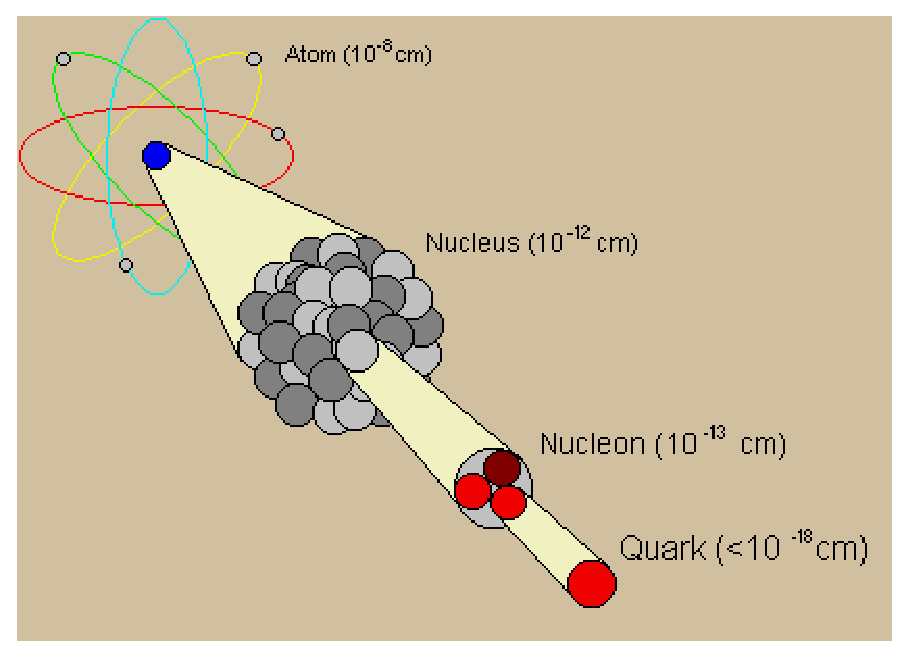
\includegraphics[type = eps, ext = .eps, scale = 1, bb = 0 0 420 300]{figs/atomo}
\end{slide}

\begin{slide}
\begin{center}
O Big-bang

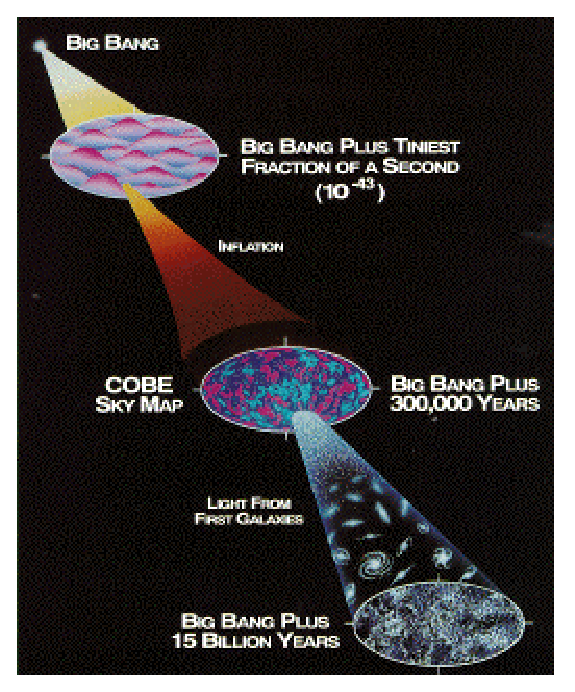
\includegraphics[type = eps, ext = .eps, scale = 1, bb = 0 0 260 316]{figs/bang}                

Os an�is aceleradores do CERN


\includegraphics[type = eps, ext = .eps, scale = 1, bb = 0 0 248 149]{figs/lhcair}
\end{center}
\end{slide}

\begin{slide}
O detetor ATLAS

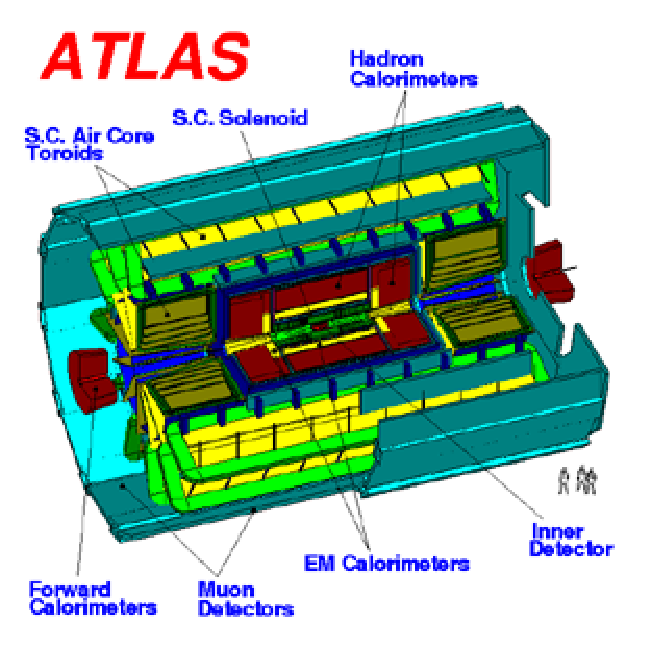
\includegraphics[type = eps, ext = .eps, scale = 1, bb = 0 0 300 295]{figs/atlasair}

Um evento reconstru�do

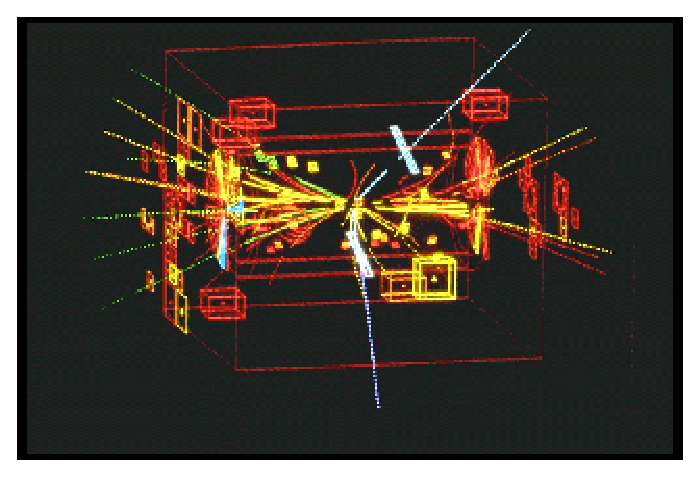
\includegraphics[type = eps, ext = .eps, scale = 1, bb = 0 0 320 213]{figs/colision}
\end{slide}

\begin{slide}
\begin{center}
Porque utilizar sistemas de valida��o ?

$\Downarrow$

Grande volume de dados

$\Downarrow$

\textcolor{blue}{\underline{Inviabilidade}} de armezenar tudo

$\Downarrow$

\textcolor{red}{\underline{Impossibilidade}} de faz�-lo
\end{center}
\end{slide}

\begin{slide}
O Sistema de \eng{Trigger} para o ATLAS

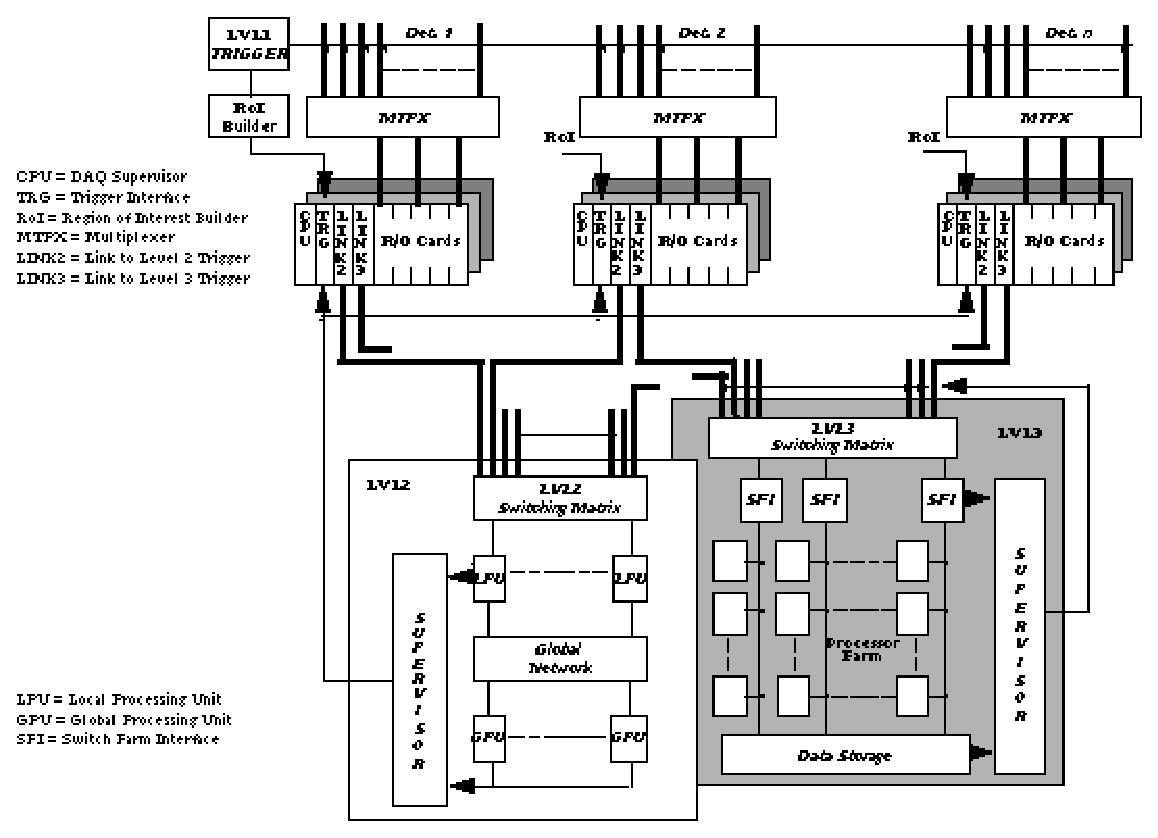
\includegraphics[type = eps, ext = .eps, scale = 0.8, bb = 0 0 540 386]{figs/trigger}
\end{slide}

\begin{slide}
Excitando os detetores

\input{picts/roi2.pic}
\end{slide}

\begin{slide}
A arquitetura A

{\tiny \input{picts/model_a2.pic}}
\end{slide}

\begin{slide}
A arquitetura B

{\tiny \input{picts/model_b2.pic}}
\end{slide}

\begin{slide}
A arquitetura C

{\tiny \input{picts/model_c2.pic}}
\end{slide}


 %% Whole introduction
\chapter{Revis�o da Literatura}
\label{chap:litera}
\index{Revis�o da Literatura}

Neste cap�tulo faremos a revis�o de algumas implementa��es e conceitos bem-sucedidos
 na descri��o e opera��o do 2\eiro n�vel de valida��o para o experimento ATLAS/LHC; 
destacam-se a utiliza��o de Redes Neurais como algor�tmo para alguns Extratores de 
Caracter�stica e unidades de Decis�o Global e, ainda, a utiliza��o de processamento 
paralelo em algumas implementa��es.

O motivo de tal direcionamento deste estudo deve-se � disponibilidade de 
equipamento com processamento distribu�do e bem-sucedidas implementa��es atrav�s de 
nosso grupo (Colabora��o Internacional CERN\-/\-COPPE\-/\-UFRJ) utilizando redes 
neurais artificiais na  
execu��o de extratores de caracter�sticas e unidades de decis�o global para a 
identifica��o de part�culas.

\section{Redes Neurais Artificiais e o processamento global para o segundo n�vel de
\eng{trigger}}
\index{Trigger!Level2!Redes Neurais aplicadas ao}
\index{Redes Neurais!Porque utiliz�-las no segundo n�vel de valida��o?}
\label{sec:ANN_at_globaldec}

Como elucidado na se��o~\ref{sec:level2}, o segundo n�vel de \eng{trigger} deve combinar as caracter�sticas 
vindas de diferentes subdetetores, de forma a aumentar a qualidade de classifica��o 
das part�culas. Neste est�gio � melhor n�o realizar uma identifica��o baseada em 
l�gica exclusiva, pois poderemos diminuir a qualidade de decis�o, mas gerar um outro 
conjunto de vari�veis, com probabilidades sobre a natureza da part�cula 
\cite{bock:ANN_at_level2}.

Considere o exemplo simples\index{Redes Neurais!Exemplo na classifi��o de 
part�culas} onde dois subdetetores n�o s�o correlacionados, ou 
seja, suas caracter�sticas extra�das s�o linearmente 
independentes (LI-s)\index{Independ�ncia Linear}. A forma mais ineficiente de 
fazer uma decis�o � a de classificar a part�cula segundo cada subdetetor e depois 
perfazer um ``E'' l�gico (AND) entre as classifica��es. Considere a ilustra��o 
da figura~\ref{fig:fexes} com as diferentes caracter�sticas extra�das da cada 
subdetetor (gen�rico), de tal forma que o n�vel de identifica��o para 2 tipos de 
excitadores de RoI, el�trons e jatos,  se d� com uma sobreposi��o de 10\%, o
 quer dizer que se tra�armos um corte para identifica��o em cada distribui��o 
teremos um erro m�nimo de 10\%. Neste exemplo a classifica��o exclusiva 
indicar� somente 81\% de corre��o na identifica��o das part�culas (o produto das 
probabilidades).

\begin{figure} 
 \begin{center}
 \caption{A distribui��o de caracter�sticas para cada subdetetor gen�rico. Os 
subsistemas s�o LI-s.} 
 \label{fig:fexes} 
 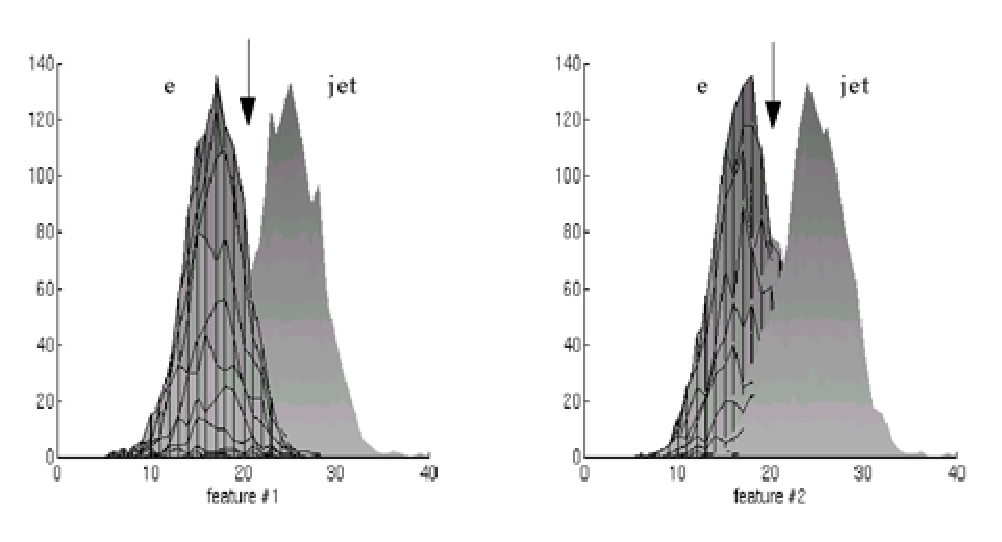
\includegraphics[type = eps, ext = .eps, scale = 0.9, bb = 0 0 464 243]{figs/fex_eg}
 \end{center}
\end{figure} 

A decis�o poder� ser melhor tomada se as duas caracter�sticas forem analisadas 
juntas, em um espa�o bidimensional (figura~\ref{fig:fex_bidim}). Cortando com um plano
como � mostrado, ambos os tipos de part�culas s�o 96\% corretamente classificadas. 
Estes tipos de cortes s�o realizados tamb�m por estruturas de Redes Neurais 
Artificiais utilizando a fun��o identidade como a fun��o de transfer�ncia para 
os neur�nios. Se o n�mero de subdetetores crescer, a diferen�a entre estas duas 
maneiras de classifica��o ficar� mais expl�cita, como � poss�vel observar na 
tabela~\ref{tab:efici_ann}. Neste teste foi considerado que todas as caracter�sticas 
foram extra�das de subsistemas LI-s, assim sendo, n�o houve necessidade da utiliza��o de
camadas escondidas.

\begin{figure} 
 \begin{center}
 \caption{Exemplo de classifica��o num espa�o bidimensional} 
 \label{fig:fex_bidim} 
 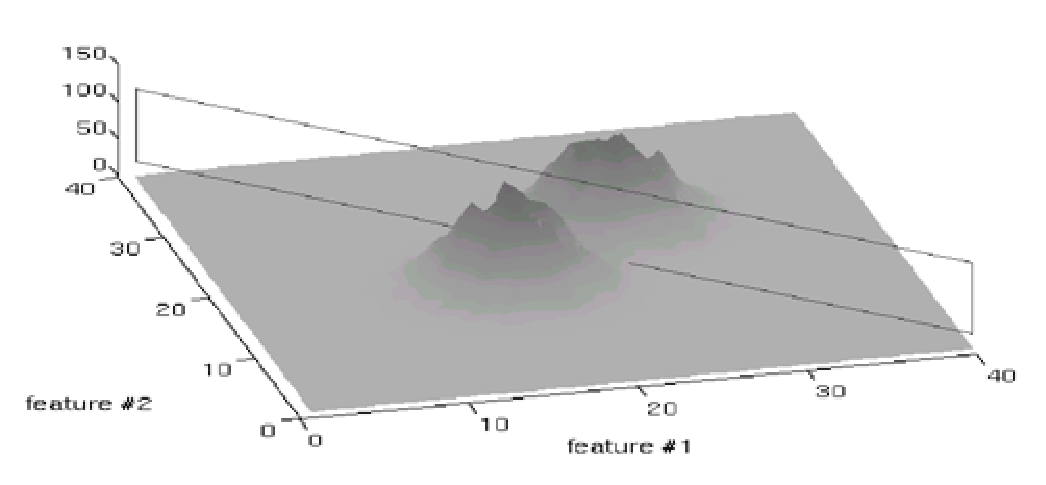
\includegraphics[type = eps, ext = .eps, scale = 0.85, bb = 0 0 485 216]{figs/fex_bid}
 \end{center}
\end{figure} 

\begin{table}
 \begin{center}
 \caption{Tabela de efici�ncias para uma classifica��o utilizando um ``E'' l�gico e 
Redes Neurais Artificiais simples, sem camadas escondidas.}
 \label{tab:efici_ann}
 \begin{tabular}{|c||c|c|}
 \hline
 N�mero de Detetores & Classifica��o com ``E'' l�gico & Classifica��o com ANN \\ 
 \hline \hline
 1 & 90\% & 90\% \\ \hline 
 2 & 81\% & 96.5\% \\ \hline 
 3 & 73\% & 98.8\% \\ \hline 
 4 & 65\% & 99.4\% \\ \hline 
 5 & 59\% & 99.8\% \\ \hline 
 \end{tabular}
 \end{center}
\end{table}\index{Redes Neurais!Tabela comparativa com se\-pa\-ra\-��o cl�s\-si\-ca}

Embora pare�a simples, a tarefa para a identifica��o de part�culas � um processo 
que envolve caracter�sticas extra�das dos dados de um n�mero de subdetetores menor 
que o n�mero de caracter�sticas\footnote{O n�mero de detetores est� entre 4 e 6 e o 
de caracter�sticas, entre 12 e 15.}, portanto, algumas destas s�o linearmente 
dependentes (LD-s)\index{Depend�ncia Linear}. Para m�xima efici�ncia na separa��o com vari�veis LD-s a 
utiliza��o de camadas escondidas � necess�ria. A figura~\ref{fig:LD_vars_and_ANNS} 
mostra o resultado de separa��o obtida sobre dados LD-s utilizando 3, 2 ou nenhum 
neur�nio na camada escondida.

\begin{figure} 
 \begin{center}
 \caption{Classifica��o em um espa�o de vari�veis linearmente dependente.} 
 \label{fig:LD_vars_and_ANNS} 
 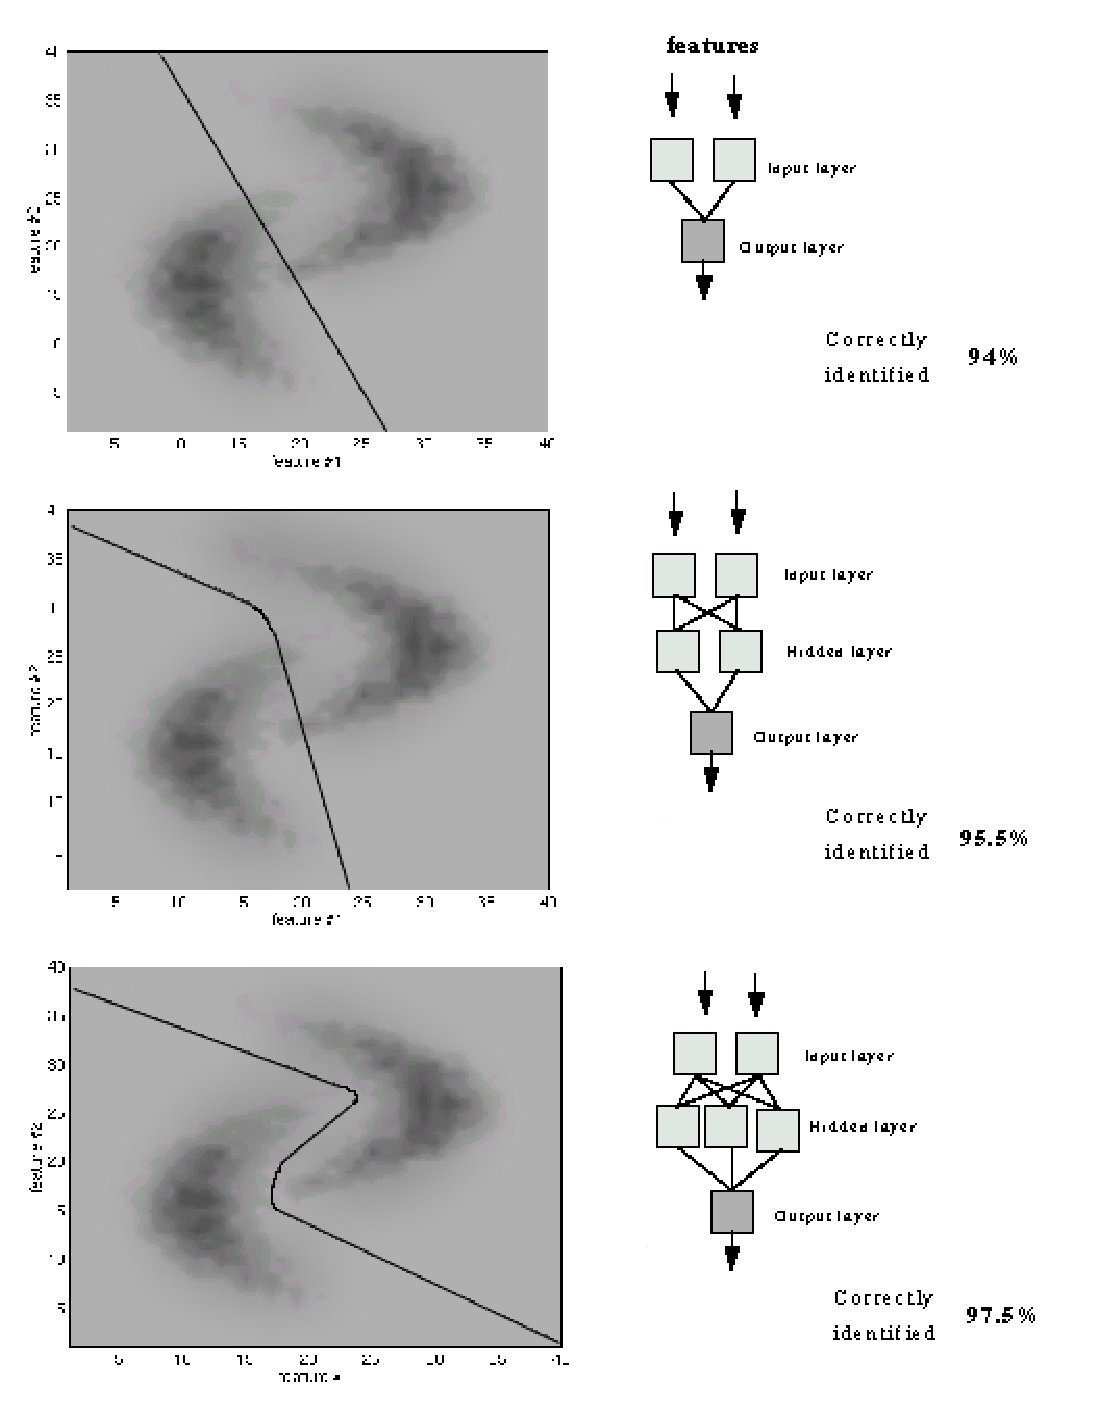
\includegraphics[type = eps, ext = .eps, scale = 0.8, bb = 0 0 511 661]{figs/annhid}
 \end{center}
\end{figure} 

\paragraph{Conclus�o:} O processamento de Decis�o Global ter� �tima efici�ncia se 
utilizarmos Redes Neurais Artificiais (ANN-s) ao inv�s de algoritmos basedos em 
classifica��o exclusiva, devido ao n�mero de subsistemas e vari�veis envolvidas. Em 
raz�o da depend�ncia entre as vari�veis dos diversos subsistemas parece inevit�vel 
a utiliza��o de ao menos uma camada escondida em uma rede neural simples, 
diretamente conectada (\eng{feed forward}).

Em particular, resultados com redes na configura��o 12-6-4, isto �, 12
entradas, 6 neur�nios na camada escondida e 4 na de sa�da t�m se mostrado satisfat�rios onde
tempo de processamento e efici�ncia s�o fatores dominantes como � poss�vel ver em 
\cite{sx:gldec}. O n�mero de sa�das � fortemente dependente da quantidade de 
part�culas diferentes que se deseja identificar no processamento da RoI. No 
caso espec�fico supracitado a identifica��o se fez por uma separa��o entre 4 
diferentes tipos de part�culas (el�trons, jatos, p�ons e m�ons).

Devemos destacar ainda que redes neurais s�o capazes de encontrar correla��es em 
espa�os multi-dimensionais ainda que na presen�a de grande quantidade de ru�do. 
Redes Neurais artificiais tamb�m podem ser muito competitivas onde pre�o e robustez 
s�o fatores delimitantes.

\section{A utiliza��o de ambientes de processamento distribu�do para o segundo n�vel de
 \eng{trigger}}
\index{Paralelismo!Porque utilizar?}

Devido �s altas taxas de eventos a que ser� submetido o segundo n�vel de 
\eng{trigger} (muitos Gigabytes por segundo e uma lat�ncia m�xima presumida de 1ms), a 
decomposi��o do problema atrav�s de paraleliza��o das atividades 
parece apontar um caminho para a solu��o. Esta
paraleliza��o pode ser implementada em 2 n�veis:
\begin{enumerate} 
 \item Na paraleliza��o de uma atividade simples como a extra��o de uma 
caracter�stica ou a identifica��o de uma part�cula, de modo a reduzir a lat�ncia do 
processamento localizado; e
 \item Na paraleliza��o de uma classe de atividades ou de todo o processamento para 
este n�vel, por exemplo, a extra��o de 
caracter�sticas utilizando uma \eng{farm} de processadores operando em paralelo 
sobre dados de diferentes RoI-s, reduzindo a lat�ncia do processamento como um todo e
 n�o localmente como no item anterior.
\end{enumerate}

Os dois tipos de paraleliza��o levam a diferentes enfoques de 
implementa��o\index{Paralelismo!enfoques}: no 
primeiro teremos um algoritmo baseado na taxa de dados (\eng{Data 
Driven})\index{Paralelismo!Data
Driven Approach}  de entradab visto que a 
paraleliza��o � feita de modo a reduzir as lat�ncias individuais, reduzindo  
a lat�ncia global do processo para cada evento. Nesta implementa��o deve-se utilizar  
uma arquitetura capaz de sustentar a taxa de dados, como em 
\cite{bock:cpp_at_level2}.

No segundo enfoque, a lat�ncia dos processos individuais n�o � demasiado importante, 
visto que poderemos compensar uma maior lat�ncia com a utiliza��o de mais 
processadores naquele n�vel de processamento. Este tipo de implementa��o � conhecido
 como \eng{Asynchronous Processor Farms 
Implementation}\index{Paralelismo!Asynchronous Approach} ou Implementa��o em 
\eng{farms} de processadores ass�ncronos. O assincronismo vem do fato das atividades
 paralelas serem independentes quanto ao tempo de execu��o entre si, podendo ser 
executadas totalmente livres do final (ou come�o) de processamento de qualquer evento
ou dado em qualquer outra unidade de processamento.

No caso do segundo n�vel em espec�fico\index{Paralelismo!Para o segundo n�vel}, 
podemos enxergar paralelismo em  
algumas das atividades realizadas e no processamento como um todo tamb�m. Para 
algoritmos de extra��o de caracter�sticas em calor�metros, t�cnicas de processamento 
paralelo  
ass�ncrono t�m se mostrado eficientes no atendimento das taxas de entrada do 
experimento, como � poss�vel ler em \cite{sx:fe}. 

Para as unidades de Decis�o Global, a utiliza��o de redes neurais artificiais t�m 
mostrado vantagem, como explicita a se��o~\ref{sec:ANN_at_globaldec}. Redes Neurais 
s�o algoritmos altamente paraleliz�veis por serem baseados em multiplica��es e somas 
vetoriais totalmente independentes ao n�vel de cada camada\footnote{� claro que os 
resultados da camada de ordem $n$ dependem dos resultados da camada de ordem 
$n-1$ e, sendo assim, n�o podemos tornar isto concorrente, ou seja, o processamento 
ainda deve ser feito camada a camada.}. Ainda, otimiza��es podem ser realizadas a 
n�vel ass�ncrono utilizando-se mais de uma rede para o processamento global.

Por fim, as atividades do segundo n�vel como um todo s�o paraleliz�veis visto a 
independ�ncia entre diferentes eventos. Estes podem ser processados 
independentemente (e, desta forma, ass�ncronamente) uns dos outros, sem perda 
de informa��es, de forma que a lat�ncia 
para cada evento possa ser aumentada proporcionalmente do valor alvo de 1ms para 
outro valor maior, dependendo de quantos forem os n�s de processamento adicionados. 
Este enfoque,  
� claro, reduz a necessidade de otimiza��o dos subn�veis de processamento internos 
ao segundo n�vel, como � o caso do enfoque baseado na taxa de dados (\eng{Data Driven 
Approach}).

\subsection{DSP-s}
\index{DSP-s!Utilidade}

\eng{Digital Signal Processors} (processadores digitais de sinais) n�o s�o mais do 
que r�pidos processadores matem�ticos que executam fun��es aritm�ticas b�sicas e 
outras fun��es complexas com poucos pulsos de \eng{clock}. Alguns DSP-s como o 
ADSP-21020 da Analog Devices podem processar em apenas 1 ciclo de \eng{clock} uma multiplica��o 
entre n�meros reais(ou pontos flutuantes).

Vantagens na utiliza��o de DSP-s s�o expl�citas quando o processamento depende do 
c�lculo de muitas vari�veis. No caso do processamento para o segundo 
n�vel, existem muitos subn�veis em que � poss�vel atingir uma redu��o da lat�ncia de
processamento utilizando-se DSP-s como processadores centrais do subn�vel \cite{bock:cpp_at_level2}.
Este � o caso da maioria dos extratores de caracter�stica e das unidades de decis�o 
global, se desenhados como Redes Neurais Artificiais.

\section{Arquiteturas para o segundo n�vel de \eng{trigger}}
\index{Trigger!Level2!Arquiteturas}

Limita��es de tamanho e custo podem nos levar a 3 poss�veis arquiteturas mutuamente 
exclusivas para o segundo n�vel de processamento\cite{level2:tsr}:
\begin{itemize} 
 \item{\bf Modelo A:} Utiliza uma parti��o local/global do segundo n�vel de processamento, 
com processamento at� a extra��o de caracter�sticas (inclusive) sendo realizado com 
arquitetura baseda no 
enfoque \eng{data-driven}, enquanto que o processamento global utiliza uma \eng{farm}
 de processadores utilizando o enfoque de processamento ass�ncrono;
 \item{\bf Modelo B:} Utiliza uma parti��o local/global de todo o processamento do 
segundo n�vel, fazendo uso de v�rias \eng{farms} feitas de processadores id�nticos ou
similares com extra��o de caracter�sticas paralela para cada subdetetor e para cada
RoI;
 \item{\bf Modelo C:} Uma �nica \eng{farm} de processadores realizando, cada um, o 
processamento relativo a um evento inteiro.
\end{itemize}

Estas arquiteturas seguem alguns crit�rios de funcionamento tais como n�o possuir 
lat�ncia de opera��o\footnote{Tempo de demora entre a decis�o do 1\eiro n�vel e a 
decis�o do segundo.} superior a 2 ms (modelo A) e 10 ms (modelos B e C); caso esta 
ultrapasse, o supervisor deve se responsabilizar por abortar a opera��o de valida��o 
para este evento. Estes crit�rios podem ser melhor estudados em 
\cite{level2:tsr} e \cite{level2:urd}.

\subsection{Modelo A}
\index{Trigger!Level2!Arquiteturas-Modelo A}

Neste modelo A, a informa��o de cada RoI � comunicada pelo \eng{RoI Builder} �s 
ROB-s (isto ainda � no 1\eiro n�vel). Os dados s�o ent�o ``empurrados'' atrav�s do 
pr�-processamento e cole��o de RoI-s para a extra��o de caracter�sticas. Nesta parte
de opera��o as unidades de processamento (acopladas, formando um �nico subsistema) 
dever�o suportar a mais alta taxa de eventos poss�vel. As opera��es s�o totalmente 
independentes para os dados de diferentes subdetetores. Para cada RoI, um vetor de 
dados � preparado contendo as caracter�sticas extra�das e um cabe�alho de 
identifica��o. Depois da extra��o de caracter�sticas, estes vetores s�o encaminhados
 a uma chave que � respons�vel por distribu�-los pelos processadores globais. A 
figura~\ref{fig:mod_a} pode ser elucidativa quanto ao mencionado nesta se��o.

\begin{figure} 
 \begin{center}
 \caption{Um diagrama esquem�tico para o modelo arquitetural A do segundo n�vel de 
valida��o.} 
 \label{fig:mod_a} 
 \input{picts/model_a.pic}
 \end{center}
\end{figure} 

\subsection{Modelo B}
\index{Trigger!Level2!Arquiteturas-Modelo B}

Neste modelo B, a informa��o de cada RoI � passada ao supervisor que controla {\bf 
todo} o fluxo de dados. Os dados de cada RoI s�o passados dos ROB-s atrav�s do 
pr�-processamento e cole��o de RoI-s a uma chave que se encarrega de passar os dados
 relativos a cada RoI para extratores de caracter�sticas. Nesta fase, os subsistemas
 relativos a cada subdetetor s�o totalmente independentes, podendo ter seus pr�prios
 supervisores locais. As caracter�sticas 
extra�das s�o, ent�o, passadas atrav�s de outra chave (que re�ne as caracter�sticas 
extra�das de cada subdetetor sobre uma mesma RoI), que repassa estes dados �s 
unidades de decis�o global. A figura~\ref{fig:mod_b} mostra um diagrama ilustrativo.

\begin{figure} 
 \begin{center}
 \caption{Um diagrama esquem�tico para o modelo arquitetural B do segundo n�vel de 
valida��o.} 
 \label{fig:mod_b} 
 \input{picts/model_b.pic}
 \end{center}
\end{figure} 

\subsection{Modelo C}
\index{Trigger!Level2!Arquiteturas-Modelo C}

Neste modelo C, a informa��o � passada a um supervisor central que dedica um dos 
processadores de uma \eng{farm} homog�nea a todo o processamento do evento. Este 
processador controla todo o fluxo de dados da RoI pelos ROB-s e pelas unidades de 
pr�-processamento e cole��o de RoI-s. Os dados, depois de coletados, seguem a uma 
chave que os repassa ao devido processador de evento, para que este realize a extra��o
 de caracter�sticas e a decis�o global. A figura~\ref{fig:mod_c} mostra um diagrama 
ilustrativo.

\begin{figure} 
 \begin{center}
 \caption{Um diagrama esquem�tico para o modelo arquitetural C do segundo n�vel de 
valida��o.} 
 \label{fig:mod_c} 
 \input{picts/model_c.pic}
 \end{center}
\end{figure} 

\section{Concluindo alguns pontos...}
\index{Revis�o da Literatura!conclus�o}

� poss�vel utilizar ANN-s para desenhar alguns subsistemas do segundo n�vel de 
valida��o, em especial Unidades de Decis�o Global e Extratores de Caracter�sticas 
para Calor�metros. Estas redes especializadas no reconhecimento de padr�es podem ter sua 
lat�ncia reduzida se utilizarmos computa��o distribu�da uma vez que seu algoritmo � 
altamente paraleliz�vel. Ainda, se utilizarmos DSP-s como processadores centrais de 
alguns destes subsistemas poderemos nos beneficiar de sua alta performance 
computacional em algoritmos envolvendo repetidos c�lculos.

A paraleliza��o da aplica��o (ainda que complexa) poder� acontecer em 2 inst�ncias: 
na primeira,  
local, h� uma paraleliza��o buscando a otimiza��o de um algoritmo utilizado em 
um subsistema, de forma a atender �s taxas de entrada e lat�ncia m�ximas deste 
subsistema; chamamos este enfoque de \eng{data-driven} uma vez que os dados fluir�o 
por estes subsistemas sem restri��es ou controle, j� que estes suportar�o as taxas de 
entrada m�ximas. Na segunda inst�ncia, global, acontece uma paraleliza��o de subsistemas 
id�nticos (exemplo: Extratores de Caracter�stica) de forma que a lat�ncia m�xima para
cada evento seja aumentada proporcionalmente ao n�mero de processadores 
anexados. Em particular a paraleliza��o em primeira inst�ncia n�o ser� aqui 
utilizada visto que equipamento espec�fico para cada subsistema paraleliz�vel � 
requerido. Utilizaremos, no entanto, o conceito de paraleliza��o global, 
ou em segunda inst�ncia como veremos mais a frente.

Existem v�rios modelos para a implementa��o do segundo n�vel, cada um com suas 
vantagens e desvantagens, embora de uma forma geral bem plaus�veis. Para fins 
e objetivos deste projeto, no entanto, nos concentraremos no modelo B. O modelo A 
requer utiliza��o de processamento  
diversificado para a camada de pr�-processamento, cole��o de RoI-s e Extra��o de 
Caracter�sticas, o que n�o ser� poss�vel, pois somente dispomos de 16 processadores em 
nossa m�quina (v�-la-emos em detalhes mais adiante) que ter�o seus potenciais 
subaproveitados se os utilizarmos em uma paraleliza��o local ou em primeira 
inst�ncia.

O modelo C exige um chaveamento a partir dos ROB-s utilizando uma chave muito r�pida
(tecnologia ATM), que tamb�m n�o se encontra em nosso poder. A arquitetura B, no 
entanto, nos  
parece mais adpt�vel ao equipamento dispon�vel (TELMAT TN310) e que queremos 
avaliar; sendo assim, 
tentaremos abordar o problema e construir o simulador baseado neste desenho. 
Lembramos que queremos atingir 2 metas aqui: a primeira � construir um 
sistema de valida��o, a segunda, testar a tecnologia contida em uma TN310 de 
forma a avaliar globalmente arquitetura e equipamento para a realiza��o do segundo 
n�vel de valida��o para o experimento ATLAS\-/\-LHC.
 
No que se segue exporemos em detalhes alguns dos conceitos, materiais e m�todos 
utilizados neste projeto, isto �, Redes Neurais Artificiais, a m�quina 
mencionada - Telmat TN310, os dados utilizados e alguns conceitos de paralelismo.

 %% Documentation Revision
%% This file contains 6 slides
\begin{slide}
Redes Neurais Artificiais - O neur�nio artificial

\begin{center}
{\tiny \input{picts/neuronc.pic}}
\end{center}
RNA multi-camadas

\begin{center}
{\tiny \input{picts/multi.pic}}
\end{center}
\end{slide}

\begin{slide}
O Sistema TN310

\begin{itemize} 
 \item Processamento Distribu�do
 \item 16 n�s independentes
 \item Mem�ria Local (MIMD)
 \item HTRAM-s tamanho 4
 \begin{enumerate} 
  \item T9000
  \item ADSP 21020 (196Kbytes)
  \item 8Mbytes RAM
  \item 256Kbytes \eng{shared}
 \end{enumerate}
 \item Totalmente conectado atrav�s de chaves STC104
\end{itemize}
\end{slide}

\begin{slide}
O T9000

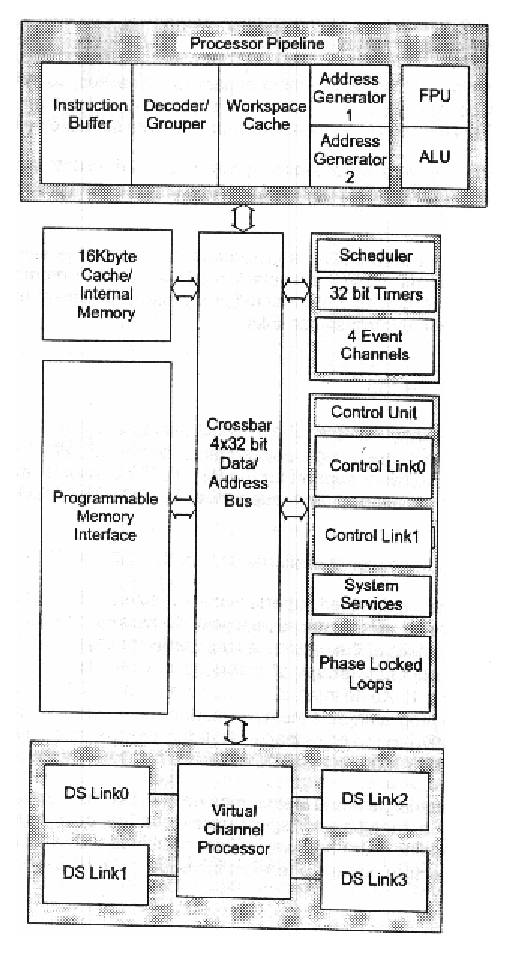
\includegraphics[type=eps, ext=.eps, bb= 0 0 228 441]{figs/T9000}
\end{slide}

\begin{slide}
O ADSP 21020

\end{slide}

\begin{slide}
A conex�o entre os n�s na TN310

{\tiny \input{picts/connect2.pic}}
\end{slide}

\begin{slide}
N�veis de programa��o

\begin{center}
{\tiny \input{picts/layer.pic}}
\end{center}

Comunica��o por canais
\begin{center}
{\tiny \input{picts/chan_op2.pic}}
\end{center}
\end{slide}


 %% Theoretical Fundaments, Methods and Materials used at this project
%% This file contains 9 slides
\begin{slide}
Modelo de neur�nio utilizado

\begin{center}
{\tiny \input{picts/neuronc.pic}}
\end{center}

A rede para a GDU
\begin{center}
{\tiny \input{picts/gdu_net.pic}}
\end{center}
\end{slide}

\begin{slide}
\begin{center}
Tabela de convers�o

{\tiny \input{picts/lut_ex2.pic}}

GDU em paralelo

{\tiny \input{picts/gdu_full.pic}}
\end{center}
\end{slide}

\begin{slide}
A comunica��o com os escravos

{\tiny \input{picts/shake.pic}}

O supervisor (fluxograma)
z
\begin{center}
{\tiny \input{picts/sup_flow.pic}}
\end{center}
\end{slide}

\begin{slide}
{\small
Resultados para a GDU
\begin{itemize} 
 \item O tempo de processamento para uma RoI da GDU rodando em apenas 1 n� � de 200$\mu$s
 \item Alocando o supervisor no n� zero e 15 escravos o tempo de processamento por 
RoI � de 30,3$\mu$s (\eng{speed-up} = 6.6)
 \item Alocando o supervisor no n� 15 e 15 escravos o tempo de processamento cai 
para 27$\mu$s (\eng{speed-up} = 7.4)
\end{itemize}
Conclus�es
\begin{itemize} 
 \item Tabela de convers�o � eficiente - reduzimos o tempo de processamento sem 
perder efici�ncia
 \item A aloca��o ``inteligente'' de tarefas leva a melhores resultados
 \item \eng{speed-up} - Bom desempenho, mas � o m�ximo ? 
\end{itemize}}
\end{slide}

\begin{slide}
� implementar no 2\eiro n�vel

{\tiny \input{picts/mod_bi2.pic}}
\end{slide}

\begin{slide}
Generaliza��o

\begin{center}
{\tiny \input{picts/top_tn.pic}}
\end{center}
\end{slide}

\begin{slide}
\label{slide:implementa}
Implementa��o usando os 16 n�s

{\tiny \input{picts/sim_v2a2.pic}}
\end{slide}

\begin{slide}
Resultados para a vers�o em apenas 1 n�
\begin{itemize} 
 \item N�o leva em considera��o tempo de distribui��o (necess�rio)
 \item Tempo para uma RoI = 1320$\mu$s
\end{itemize}
Resultado para a vers�o concorrente 1 (aloca��o aleat�ria)

$\Rightarrow$ Tempo para uma RoI = 830$\mu$s (\eng{speed-up} = 1,6)

Resultado para a vers�o concorrente 2 (aloca��o ``inteligente'')

$\Rightarrow$ Tempo para uma RoI = 690$\mu$s (\eng{speed-up} = 1,9)

Resultados para a vers�o concorrente 3 (distribui��o sequencial)

$\Rightarrow$ Tempo para uma RoI = 390$\mu$s (\eng{speed-up} = {\bf 3,4 !})
\end{slide}

\begin{slide}
Conclus�es
\begin{itemize} 
 \item Sabendo que \eng{speed-up} m�ximo � 4 ($//$ dados e fluxo) atingimos 85\% do 
m�ximo
 \item Melhora de 43\% da vers�o 3 para a vers�o 2
 \item Considerando 1 e\-ven\-to $\approx$ 5 RoI-s $\Rightarrow$ 2ms\-/\-e\-ven\-to (500Hz)
 \item Lentid�o $\Rightarrow$ Tempo de distribui��o dos dados para fex-s $\Rightarrow$ 96\% do 
tempo total de aplica��o
 \item Atingimos o m�ximo desta tecnologia ?
\end{itemize}
\end{slide}

 %% Project implementation and constraints at TN310
\chapter{Resultados obtidos e Conclus�es}
\label{chap:results}

Neste cap�tulo, estaremos expondo os resultados obtidos com as implementa��es expostas
no cap�tulo anterior. Para todas as implementa��es, consideramos o \eng{speed-up} em 
rela��o a uma vers�o simples da aplica��o, isto �, rodando em um �nico processador. 
Tamb�m � feita uma revis�o dos tempos de comunica��o e afins.

Inicialmente, repassaremos testes realizados sobre o tempo de comunica��o do sistema 
TN310. Estes testes visaram a um entendimento operacional do tempo de processamento 
dispendido durante comunica��es entre aplica��es. Na segunda se��o, traremos 
resultados para a aplica��o do sistema de decis�o global e na se��o seguinte, 
exporemos os resultados e conclus�es para a simula��o do sistema de valida��o.

\section{Teste de comunica��es}
\secl{time}

Em equipamentos com n�mero de n�s de processamento consider�vel � necess�rio o 
entendimento pleno do sistema de comunica��o utilizado. Quando menciona-se 
``Entendimento Pleno" quer se acentuar que para uma otimiza��o das rotinas h�
 a necessidade de o programador desenvolver uma ``afinidade'' muito grande com o 
equipamento. Esta afinidade traduz-se no entendimento de todos os detalhes de 
funcionamento do sistema, sejam eles de alto ou de baixo n�vel.

O processo de comunica��o entre os diversos n�s de processamento no sistema TN310 
n�o � diferente,  
isto �, ele possui uma interface de alto n�vel (como as fun��es da 
tabela~\tabr{channel.h}) e uma interface de baixo n�vel, inerente ao sistema. A 
interface de alto n�vel � respons�vel pelo processo de comunica��o em si, mas os 
motivos pelos quais alguns tipos de comunica��o s�o diferentes de outros � um ponto 
que somente pode ser explicado com o entendimento do sistema operando em baixo 
n�vel. Desta forma, antes de entrarmos nos resultados destes testes propriamente,
abordaremos alguns aspectos na forma de comunica��o entre os diversos n�s HTRAM do 
sistema TN310.

\subsection{Introdu��o ao sistema de comunica��es}

O sistema de comunica��es da TN310 � totalmente baseado no conceito de chaveamento 
ass�ncrono de pacotes (\eng{Asynchronous Packet Switch}). Este tipo de sistema pode 
aumentar a ``performance'' em ambientes maiores, como � caso. Ele se baseia na utiliza��o
 de uma chave r�pida (STC104) para que haja a distribui��o de pacotes pela rede de 
forma mais r�pida e livre de erros poss�vel. Estas chaves podem rotear at� 32 
pacotes diferentes ao mesmo tempo, vindo de quaisquer 32 localidades distintas e 
indo para outras 32 localidades tamb�m distintas.

A id�ia �, na verdade, bem simples. Quando uma informa��o deseja ser mandada de um 
ponto a outro, a tarefa no ponto emissor envia uma mensagem ao processador virtual de
 canais local indicando o endere�o e o tamanho do dado a ser mandado. O processador 
de canais divide o dado a ser enviado em v�rios pacotes de tamanho predeterminado. 
Ap�s esta divis�o, a cada pacote � adicionado um cabe�alho contendo a loca��o-destino 
e a rota para o pacote. O pacote � enviado a uma chave que interpreta a primeira parte do 
cabe�alho e envia o pacote para o n� correto, removendo a parte do cabe�alho 
referente � rota j� informada e deixando exposta a parte do cabe�alho referente ao 
n�-destino do pacote. Ao chegar ao n�-destino,
cada pacote � autenticado (i.e., verifica-se se realmente se est� esperando 
tal informa��o e se o cabe�alho est� correto) e um reconhecimento (\eng{acknowledgement}) 
� enviado para que o pr�ximo pacote seja mandado, se este for o caso.

No caso de o pacote ter que passar por 2 chaves, 3 cabe�alhos s�o inseridos a cada 
pacote. Este ser� roteado atrav�s de 2 chaves e ocorrer�o 2 remo��es de 
cabe�alhos (\eng{header deletion}) e apenas um ser� utilizado novamente no n� destino.
Desta forma, � poss�vel garantir que poderemos criar um n�mero muito grande de 
canais virtuais. Comunica��o utilizando canais virtuais nada mais � do que 
comunica��o feita com pacotes de dados  intercalados simulando um sistema com maior 
n�mero de conex�es do que realmente existem.

Quando � dito que h� uma multiplexa��o dos canais, quer-se dizer que, uma
vez que s�o dividos em pacotes, os dados a serem enviados podem ser intercalados, 
gerando uma rede de multiplexa��o de pacotes e, assim, satisfazendo um grande n�mero 
de canais simult�neos, chamados virtuais. 

A figura~\figr{header_del} pode ser elucidativa quanto � remo��o de cabe�alhos.

\begin{figure} 
 \begin{center}
 \caption{O processo de dele��o de cabe�alho em uma rede com chaveamento ass�ncrono 
de pacotes.} 
 \figl{header_del} 
 \input{picts/head_del.pic}
 \end{center}
\end{figure} 

\paragraph{Concluindo.} A TN310 � um sistema distribu�do com 16 n�s de processamento
tipo HTRAM totalmente conectados atrav�s de uma rede de chaves ass�ncronas. A 
comunica��o nesta rede � feita atrav�s canais descritos em \eng{software} (InMOS C), mas
implementados via \eng{hardware} atrav�s de um sistema de canais virtuais cujo 
processador central � o VCP (Processador de Canais Virtuais). O VCP divide a 
informa��o a ser mandada em pacotes e a cada pacote adiciona um n�mero de cabe�alhos
proporcional ao n�mero de n�s por onde o pacote passar�. Assim sendo, se o pacote 
tiver que passar por 2 chaves adicionar-se-�o 3 cabe�alhos (2 para as chaves e 1 para 
o n�-destino). Os pacotes s�o enviados intercaladamente com outros pacotes de outras
informa��es que tamb�m est�o sendo enviadas. Isto cria uma rede de canais virtuais.

\subsection{Os testes}

Levando em considera��o que estaremos alocando em cada n� de processamento uma �nica
tarefa seq�encial, isto �, sem que dispare processos concorrentes, podemos chegar � 
conclus�o que todos os DS-Links estar�o � disposi��o da aplica��o para a transmiss�o
de dados. Isto maximiza a utiliza��o dos meios de comunica��o de cada n�. Estamos 
interessados em entender 2 pontos na opera��o do sistema:
\begin{enumerate} 
 \item Qual � o tamanho de cada pacote mandado por vez?
 \item Quanto tempo demora para que pacotes sejam enviados a diferentes n�s de 
processamento?
\end{enumerate}
   
A primeira quest�o tem um motivo pr�tico: sabendo o tamanho do pacote, 
podemos maximizar seu uso. A segunda quest�o se refere ao tempo gasto para que 
enviemos uma quantidade fixa de dados de um ponto para outro do sistema. Ao saber 
isto, estaremos aptos a tomar melhores decis�es sobre a aloca��o de processos e 
avaliar melhor o quadro de opera��o de uma aplica��o.

O teste realizado consiste em mandar dados de diferentes tamanhos para 
diferentes n�s de processamento e medir o tempo gasto durante esta transfer�ncia. 
Saberemos que este tempo representa a melhor condi��o poss�vel de opera��o, onde os 4
DS-Links estar�o � disposi��o do processo de comunica��o. O envio de dados ocorreu 
de forma iterativa, embora tenhamos descontado o tempo de itera��o no final do 
processo. A itera��o serviu para que pud�ssemos avaliar mais precisamente o tempo de
comunica��o para os diversos tamanhos de dados.

Os resultados encontram-se na tabela~\tabr{time}. A tabela exp�e na horizontal o 
tempo (em $\mu$segundos) para que haja a transmiss�o do n�mero de bytes indicados � 
direita atrav�s de 4 tipos diferentes de conex�o. Cada tipo representa o n�mero de 
chaves existentes entre os n�s de processamento. Existem diferentes tipos de 
conex�es, como foi visto na se��o~\secr{connect}. A conex�o do tipo 1 representa a
 conex�o entre dois n�s onde ocorre apenas uma chave; a do tipo 2, 2 chaves e, 
assim, sucessivamente, at� 4 chaves (conex�o entre os n�s 0 e 8).

\begin{table}
 \caption[Os tempos gastos para os diversos tamanhos de dados comunicados a 
diferentes n�s de processamento.]{Os tempos gastos para os diversos tamanhos de dados 
comunicados a diferentes n�s de processamento. Tempos em microssegundos e tamanho em 
bytes ou pacotes de 32 bytes.} 
 \tabl{time}
 \begin{center}
  \begin{tabular}{|r|r|c|c|c|c|} \hline
Tamanho (bytes)& Tamanho (pacotes) & Tipo 1 & Tipo 2 & Tipo 3 & Tipo 4 \\ \hline \hline
1 at� 32 & 1 & 10,2 & 12,1 & 13,8 & 15,5 \\ \hline
33 at� 64 & 2 & 16,9 & 20,6 & 24,0 & 27,6\\ \hline
65 at� 96 & 3 & 23,5 & 28,9 & 34,2 & 39,5\\ \hline
100 & 4 & 30,2 & 37,5 & 44,6 & 51,8 \\ \hline
150 & 5 & 37,2 & 46,0 & 54,7 & 63,6 \\ \hline
200 & 7 & 50,5 & 62,9 & 75,3 & 87,6 \\ \hline
250 & 8 & 57,2 & 71,4 & 85,4 & 99,5 \\ \hline
300 & 10 & 70,8 & 88,2 & 106 & 123 \\ \hline
350 & 11 & 77,3 & 96,7 & 116 & 136 \\ \hline
400 & 13 & 90,6 & 114 & 136 & 159 \\ \hline
450 & 15 & 104 & 130 & 157 & 183 \\ \hline
500 & 16 & 111 & 139 & 167 & 195 \\ \hline
550 & 18 & 124 & 156 & 188 & 219 \\ \hline
600 & 19 & 131 & 164 & 198 & 231 \\ \hline
650 & 21 & 114 & 181 & 218 & 255 \\ \hline
700 & 22 & 151 & 190 & 228 & 261 \\ \hline
750 & 24 & 164 & 206 & 249 & 291 \\ \hline
800 & 25 & 171 & 215 & 255 & 303 \\ \hline
850 & 27 & 184 & 232 & 219 & 327 \\ \hline
900 & 29 & 197 & 245 & 300 & 351 \\ \hline
950 & 30 & 204 & 257 & 310 & 363 \\ \hline
1000 & 32 & 217 & 274 & 331 & 387 \\ \hline
1500 & 47 & 317 & 400 & 484 & 567 \\ \hline
2000 & 63 & 424 & 535 & 647 & 758 \\ \hline
2500 & 79 & 531 & 670 & 810 & 950 \\ \hline
3000 & 94 & 631 & 797 & 964 & 1130 \\ \hline
3500 & 110 & 737 & 931 & 1130 & 1320 \\ \hline
4000 & 125 & 838 & 1060 & 1280 & 1500 \\ \hline
4500 & 141 & 944 & 1190 & 1440 & 1690 \\ \hline
5000 & 157 & 1050 & 1330 & 1610 & 1880 \\ \hline
5500 & 172 & 1150 & 1450 & 1760 & 2060 \\ \hline
6000 & 188 & 1260 & 1590 & 1920 & 2260 \\ \hline
6500 & 204 & 1360 & 1720 & 2090 & 2450 \\ \hline
7000 & 219 & 1460 & 1850 & 2240 & 2630 \\ \hline
7500 & 235 & 1570 & 1990 & 2400 & 2820 \\ \hline
8000 & 250 & 1670 & 2110 & 2560 & 3000 \\ \hline
8500 & 266 & 1790 & 2250 & 2720 & 3190 \\ \hline
9000 & 282 & 1900 & 2400 & 2880 & 3380 \\ \hline
9500 & 297 & 2000 & 2530 & 3040 & 3560 \\ \hline
10000 & 313 & 2120 & 2670 & 3200 & 3760 \\ \hline
  \end{tabular}
 \end{center}
\end{table}

Com este resultado, percebemos que o tamanho do pacote mencionado anteriormente � de 
32 bytes. Este valor � fixo para comunica��es em qualquer dist�ncia. Isto quer dizer
que a inclus�o de mais ou menos cabe�alhos n�o influencia no tamanho do pacote 
enviado. 

A aplica��o foi feita de forma que as tarefas escravas receptoras de dados 
sempre estariam dispon�veis para o recebimento de dados, nunca atrasando a 
tarefa-mestra. Um fator interessante � que podemos perceber que, em verdade, o que ocorre  
� uma distribui��o de pacotes. Este fato fica marcante se olharmos a 
segunda parte da tabela, que indica ``tamanho (em pacotes)''. Ao compararmos o envio 
de 1 pacote, logo utilizando 1 dos 4 DS-Links dispon�veis, o tempo de demora � um. 
Por�m, se estivermos mandando mais de um pacote, logo utilizando mais de um DS-Link,
 o tempo por pacote cai, ainda que o tempo total aumente. Isto se deve ao fato de 
que o VCP processa os dados a serem enviados seq�encialmente, o que obrigatoriamente
 nos leva a um aumento do tempo, mas vemos que o simples fato de enviar 2 pacotes 
quase simultaneamente reduz o tempo total cerca de 16\% (essa taxa reduz quanto 
maior o n�mero de chaves na conex�o chegando at� 11\%). Se enviarmos 3 pacotes a taxa 
de redu��o chega a 23\%, para 4, a 26\% e assim segue at� que esta taxa atinja o 
valor de 34\%,  
quando enviamos mais de 300 pacotes utilizando os 4 DS-Links. Esta taxa pode ser 
mencionada como taxa de satura��o, i.e., representa o m�ximo na otimiza��o de 
comunica��o ating�vel (para conex�es do tipo 1) usando 4 canais simult�neos, ao inv�s 
de apenas 1. 

Estes resultados mostram que o envio de mais de 4 pacotes nesta situa��o (uma tarefa 
por processador) parece ser uma caracter�stica interessante em termos de otimiza��o.
Os processos podem ser ajustados para que o volume de comunica��es n�o seja menor do
que 4 pacotes por vez. Pelo fato da rede estar totalmente conectada atrav�s de chaves 
ass�ncronas e os DS-Links terem cada um uma conex�o com a rede, se usarmos 
a configura��o de uma tarefa (sem processos concorrentes) por processador, nunca 
teremos congestionamento de dados. 

Depois do entendimento do processo de comunica��o e troca de dados, veremos as 
implementa��es propostas no cap�tulo~\ref{chap:project}.

\section{Resultados para a GDU}

\subsection{Replicando o JETNET}
\secl{gdu_single}

Implementamos 2 processos distintos para a unidade de decis�es globais; no primeiro 
tentamos replicar os resultados obtidos com o pacote JETNET no ambiente do sistema 
TN310 (InMOS C), usando os pesos, \eng{thresholds} e vetores de normaliza��o achados 
durante a fase de treinamento neste primeiro ambiente (JETNET). A 
tabela~\tabr{eficience_ic} mostra os resultados de efici�ncia obtidos  
utilizando o programa do ap�ndice~\ref{ap:global1}. Quando mencionamos efici�ncia de
uma RNA queremos destacar sua capacidade no reconhecimento de padr�es, assim, uma 
efici�ncia de 90\% significa que de cada 100 part�culas de um dado tipo a rede 
consegue \textbf{corretamente} identificar 90 e, assim, sucessivamente.

\begin{table}
 \caption[As efici�ncias para a rede 12-6-4 da GDU usando InMOS C.]{As efici�ncias 
para a rede 12-6-4 da GDU usando InMOS C. Os valores para $\pi^{-}$ n�o foram 
computados por n�o representarem um volume de dados expressivo. As marcas ``---'' 
indicam que n�o aconteceram part�culas daquele tipo no arquivo de entrada.}
 \tabl{eficience_ic}
 \begin{center}
  \begin{tabular}{|c|c|c|c|c|} \hline
             & $4e^{-}$ & $2e^{-}+2j$ & $2e^{-}+2\mu$ & $4\mu$ \\ \hline \hline
  $e^{-}$ & 97.45 & 99.50 & 94.75 & ---\\ \hline
  $jets$ & 93.40 & 96.13 & 96.40 & 100\\ \hline
  $\mu$ & --- & 94.44 & 100 & 99.95\\ \hline
  \end{tabular}
 \end{center}
\end{table}

O tempo de processamento m�dio por RoI foi de 200 microssegundos. Este tempo leva
em considera��o somente o processamento neuronal da RoI; a leitura e escrita em 
disco foram realizadas sem contar tempo de processamento. O casamento perfeito entre
a tabela~\tabr{eficience} e a tabela~\tabr{eficience_ic} mostra a validade da 
substitui��o do c�lculo utilizando s�ries (\raw{tanh()}) por uma tabela de convers�o. 
Esta substitui��o tamb�m reduz o tempo de processamento requerido por RoI.

\subsection{A GDU concorrente}

A segunda vers�o do programa, operando em 15 n�s no sistema TN310; foi executada em 2
configura��es: na primeira alocamos os processos como descrito na 
tabela~\tabr{aloc_v1}.

\begin{table}
 \caption{A GDU concorrente, vers�o 1 - Mapa de aloca��o de processos.}
 \tabl{aloc_v1}
 \begin{center}
  \begin{tabular}{|c|c|} \hline
  Tarefa & Processador \\ \hline \hline
  Supervisor & 0 \\ \hline
  15 GDU-s & 1 ao 15 \\ \hline
  \end{tabular}
 \end{center}
\end{table}

Optamos por esta configura��o para demostrarmos que diferentes posicionamentos dos 
processos podem nos levar a resultados bem diferentes. O tempo de processamento 
encontrado para uma ROI foi, aproximadamente, de 30,3 microssegundos. Consideramos o 
fator de   
agiliza��o da aplica��o (\eng{speed-up}) como a rela��o entre o tempo gasto para 
processar 1 RoI na aplica��o constru�da em apenas um n� do sistema TN310 e o tempo 
gasto para processar 1 RoI em qualquer outra configura��o da mesma aplica��o 
operando em mais de um n� de processamento do sistema. Neste caso, o \eng{speed-up} da 
aplica��o, quando a comparamos com a vers�o que roda em apenas 1 n� de processamento
este resultado de 30,3 $\mu s$ por RoI, fica em torno de 6,6.

Se utilizarmos a organiza��o apontada na tabela~\tabr{aloc_v2}, o tempo de 
processamento por evento cai para cerca de 27 microssegundos por RoI. Isto nos leva 
a um \eng{speed-up} de 7,4.

\begin{table}
 \caption{A GDU concorrente, vers�o 2 - Mapa de aloca��o de processos.}
 \tabl{aloc_v2}
 \begin{center}
  \begin{tabular}{|c|c|} \hline
  Tarefa & Processador \\ \hline \hline
  Supervisor & 15 \\ \hline
  15 GDU-s & 0 ao 14 \\ \hline
  \end{tabular}
 \end{center}
\end{table}

\subsection{Conclus�es sobre a unidade de decis�es globais}

Os dados recolhidos aqui, sem contar com as efici�ncias, representam a m�dia 
aritm�tica de milhares de itera��es. Isto significa que estes dados est�o t�o 
pr�ximos dos valores m�dios quanto foi poss�vel chegar. De forma nenhuma os valores 
aqui apresentados representam dados esp�rios ou ocasionais.

\paragraph{A tabela de convers�o.} A utiliza��o da tabela de convers�o provou-se 
muito eficiente como forma de substitui��o da aritm�tica complexa envolvida no 
c�lculo de fun��es como a tangente hiperb�lica. Neste caso espec�fico, a substitui��o
da fun��o implementada por expans�o em s�rie por uma tabela de convers�o mostrou-se
ideal, visto que consiguimos diminuir o tempo de processamento sem termos reduzido a 
efici�ncia de separa��o da rede.

\paragraph{O tempo de processamento em 1 n�.} O tempo de processamento por RoI em 1 
n� encontrado (200 $\mu s$) � representativo do processamento neural da RoI, n�o 
incluindo de forma alguma as rotinas de leitura e escrita dos dados de cada RoI. O 
processamento neuronal, neste caso espec�fico, consiste de 86 somat�rios, 72 
multiplica��es e 10 ativa��es. Sabendo que 1 ciclo de um processador dura no m�nimo 
1 microssegundo\footnote{Embora o \eng{clock} seja de 20MHz (50ns por pulso) cada ciclo do 
\eng{transputer} � executado em 1 microssegundo para processos em alta prioridade e em 
64ms para processos em baixa prioridade.} e que realizamos 168 opera��es distintas,
sendo que 10 delas s�o mais complexas (ativa��o da \raw{NET} dos neur�nios) dir�amos 
que o valor de 200$\mu s$ por RoI � bem satisfat�rio e coerente.

\paragraph{Aloca��o de tarefas.} Uma diferen�a de at� 10\% no tempo de processamento
 pode ser observado se realocarmos de forma eficiente os processos. Este fator 
exemplifica que o bom programador � aquele que conhece o equipamento com que 
trabalha, pois desta forma consegue aproveitar o m�ximo de cada recurso.

\paragraph{O \eng{Speed-up}.} O valor para o \eng{speed-up} de 7,4 � um bom 
resultado. O valor m�ximo para esta caracter�stica �, no caso espec�fico de 15 
escravos concorrentes, 15. Uma vez que o tempo gasto na comunica��o introduz uma 
seq�encializa��o na aplica��o, como visto na se��o \secr{data_par}, � de se esperar 
que este fator de agiliza��o se reduza drasticamente. 

De uma forma geral, a aplica��o de v�rias t�cnicas como o paralelismo de dados, a 
convers�o de valores por tabelas e a otimiza��o baseada na organiza��o de 
\eng{hardware} conseguiram multiplicar em at� 7,4 vezes a velocidade de execu��o de 
uma rede neuronal. A utiliza��o de uma m�quina de processamento distribu�do neste 
caso mostrou-se eficaz.

\section{Resultados para a implementa��o do segundo n�vel de \eng{trigger}}

Apresentaremos aqui os resultados obtidos com as 3 vers�es de implementa��o para o 
segundo n�vel de valida��o do experimento ATLAS/LHC. Destacamos aqui, como fizemos 
anteriormente, que atingimos a m�xima otimiza��o atrav�s de v�rias implementa��es 
como se seguem. 

\subsection{Resultados para o algoritmo completo rodando em apenas 1 processador}

Foi simulado o processamento completo de uma RoI, 100 vezes (para tirarmos uma 
m�dia), utilizando-se de apenas um n� de processamento. Este processamento consiste 
em, sequencialmente, extrair-se as caracter�sticas da RoI e pass�-la na rede neural 
12-6-4 das unidades de decis�o global. O tempo de processamento para cada RoI foi de 
1,7 ms em m�dia. Este processamento n�o inclui, � claro, a parte relativa �s Redes 
Locais, que s� t�m sentido de implementa��o em sistemas distribu�dos. Isto se deve 
ao fato de que Redes Locais representam processos de distribui��o e recolhimento de 
dados, o que n�o ocorre em uma vers�o seq�encial da aplica��o, pois n�o h� 
distribui��o dos dados por um sistema complexo. Os dados mant�m-se em uma �nica 
unidade de processamento por todo o tempo.

Os tempos simulados para os algoritmos de extratores estavam de acordo com os dados
da tabela~\tabr{fexor_proc}.

O valor de 1,7 ms ser� utilizado para calcularmos o \eng{speed-up} das aplica��es 
que se seguem. Utilizaremos o mesmo crit�rio de c�lculo utilizado na avalia��o da 
agiliza��o para a unidade de decis�es globais: dividiremos o tempo de processamento 
de uma RoI processada por apenas um n� pelo tempo gasto para processar uma RoI em 
configura��es que utilizem mais de um n� de processamento, como as que se seguem; 
assim, chegaremos ao que consideramos o \eng{speed-up} da aplica��o.

\subsection{Resultados para a vers�o 1}

Ao executarmos esta vers�o chegamos aos resultados contidos na 
tabela~\tabr{simul_1_results}.
 
\begin{table}
 \caption{Os resultados obtidos com a implementa��o da primeira vers�o do simulador 
para o sistema de valida��o. Totais para 500 RoI-s.}
 \tabl{simul_1_results}
 \begin{center}
  \begin{tabular}{|c|c|c|} \hline
  & Tempo ($ms$) & \% do tempo total \\ \hline \hline
  Distribui��o de dados para Extratores & 365.079 & 87,93 \\ \hline
  Perda com verifica��es redundantes & 29.580 & 7,12 \\ \hline
  Total de aplica��o & 415.189 & 100 \\ \hline
  \end{tabular}
 \end{center}
\end{table}

Podemos perceber que o maior ``gargalo'' de nossa aplica��o encontra-se na distribui��o 
de dados para os extratores de caracter�stica, somando aproximandamente 90\% do 
tempo total da aplica��o. Embora existam t�cnicas para otimizar a comunica��o entre 
tarefas, n�o h� como eliminarmos por completo ou em boa parte o tempo gasto nesta 
distribui��o. Isto se deve a fatores puramente l�gicos: a passagem de dados da 
aplica��o supervisora para os extratores de caracter�stica � necess�ria, ou n�o 
teremos aplica��o. Outro fator interessante a ser lembrado � que jamais 
conseguiremos otimizar o fluxo de dados nesta aplica��o, pois todos os canais com 
extratores de caracter�stica demandam um alto volume de dados, portanto j� 
utilizando mais de um DS-Link por vez.

O tempo de processamento para cada RoI fica em torno de 830 $\mu s$.
O \eng{speed-up} �:
\begin{displaymath}
speed-up = \frac{1700}{830} = 2,05,
\end{displaymath}
que � um valor baixo.
Tentamos a otimiza��o por realoca��o dos processos como se segue.

\subsection{Resultados para a vers�o 2}

Ao realocarmos os processos de uma forma mais eficiente, esperamos que os tempos 
gastos em comunica��o se reduzam; desta forma ter�amos um aumento do \eng{speed-up} 
da aplica��o. Os resultados est�o na tabela~\tabr{simul_2_results}. Tentamos, 
tamb�m, eliminar o tempo gasto com a verifica��o de extratores cujos os dados j� 
acabaram, tentando minimizar o tempo de processamento.

\begin{table}
 \caption{Os resultados obtidos com a implementa��o da segunda vers�o do simulador 
para o sistema de valida��o. Totais para 500 RoI-s.}
 \tabl{simul_2_results}
 \begin{center}
  \begin{tabular}{|c|c|c|} \hline
  & Tempo ($ms$) & \% do tempo total \\ \hline \hline
  Distribui��o de dados para Extratores & 335.695 & 97,58 \\ \hline
  Perda com verifica��es redundantes & 0 & 0 \\ \hline
  Total de aplica��o & 344.015 & 100 \\ \hline
  \end{tabular}
 \end{center}
\end{table}

O tempo gasto com a verifica��o de extratores parados foi totalmente retirado, ainda 
que tenhamos sofrido alguma penalidade na redu��o das dist�ncias entre os processos, 
a medida que tivemos que adicionar c�digo para a elimina��o deste tempo extra.

O tempo de processamento para cada RoI baixou para 688 $\mu s$. Isto significa que o 
\eng{speed-up} aumentou, vejamos:
\begin{displaymath}
speed-up = \frac{1700}{688} = 2,47.
\end{displaymath}

Embora estejamos pr�ximos de um aumento de 20\%, estes ajustes ainda n�o 
caracterizariam uma boa ``performance'' pelo equipamento. Visto que uma abordagem 
tentando maximizar a utiliza��o dos canais n�o aponta bons resultados, pois o �nico 
canal a ser otimizado � para a distribui��o de dados para extratores de m�ons, que 
n�o se encontram t�o distantes da otimiza��o m�xima, direcionamo-nos para a implementa��o 
utilizando a distribui��o circular de eventos, como abordado na 
se��o~\secr{simul_v3}.

\subsection{Resultados para a vers�o 3}

Esta vers�o tira proveito da sequencializa��o do processo de distribui��o de eventos
e de rotinas especiais, otimizadas para a utiliza��o na implementa��o em alto n�vel
de canais virtuais criados em \eng{hardware}, caso espec�fico do Transputer T9000.
Este conjunto de rotinas � conhecido como \raw{DirectChan-s}, e funciona de forma 
id�ntica �s rotinas da tabela~\tabr{channel.h}, apenas de forma mais r�pida.

Os resultados desta vers�o de implementa��o encontram-se na 
tabela~\tabr{simul_3_results}.
\begin{table}
 \caption{Os resultados obtidos com a implementa��o da terceira vers�o do simulador 
para o sistema de valida��o. Totais para 500 RoI-s.}
 \tabl{simul_3_results}
 \begin{center}
  \begin{tabular}{|c|c|c|} \hline
  & Tempo ($ms$) & \% do tempo total \\ \hline \hline
  Distribui��o de dados para Extratores & 194.427 & 96 \\ \hline
  Perda com verifica��es redundantes & 0 & 0 \\ \hline
  Total de aplica��o & 203.453 & 100 \\ \hline
  \end{tabular}
 \end{center}
\end{table}

O tempo para o processamento de uma RoI atinge, nesta implementa��o, cerca de 
390 $\mu s$.
O \eng{speed-up}:
\begin{displaymath}
speed-up = \frac{1700}{390} = 4,36.
\end{displaymath}

\subsection{Concluindo sobre o sistema de valida��o}

Cabe aqui uma pequena revis�o do processo de paraleliza��o como um todo; para isto 
repetiremos aqui algumas das figuras mostrando o processo de modelagem e implementa��o
da aplica��o. 

Inicialmente est�vamos diante de uma apl�ca��o de dif�cil paraleliza��o, mostrada 
na figura~\figr{mod_b_implementation} e repetida aqui na 
figura~\figr{conclusion_1}. Esta aplica��o possui 2 n�veis de paraleliza��o 
distintos, um segundo o seu fluxo, pois atua como um \eng{pipeline} processando os 
dados no sentido dos extratores para as unidades de decis�o global; e outro segundo seus 
dados. Neste caso estaremos atuando sobre um volume de dados cuja natureza e 
grandeza s�o as mesmas; poderemos, ent�o, utilizar processamento repetido para que 
agilizemos o processo como um todo.

\begin{figure} 
 \begin{center}
 \caption{O diagrama da aplica��o implementada no sistema TN310.} 
 \figl{conclusion_1} 
 \input{picts/mod_b_i.pic}
 \end{center}
\end{figure} 

A aplica��o destas duas t�cnicas neste �ltimo diagrama (figura~\figr{conclusion_1}) 
nos leva ao diagrama de tarefas da figura~\figr{conclusion_2}. Este diagrama foi 
arranjado de forma a maximizar a utiliza��o dos processadores e minimizar as cargas
sobre cada n� de processamento, balanceando o sistema.
                                                              
\begin{figure} 
 \begin{center}
 \caption{As tarefas da aplica��o.} 
 \figl{conclusion_2} 
 \input{picts/simul1.pic}
 \end{center}
\end{figure} 

O \eng{speed-up} para tal aplica��o vir�, portanto, na forma de 2 caracter�sticas 
adicionadas � execu��o do sistema, sua paraleliza��o de dados e sua paraleliza��o de
fluxo. Se somente pud�ssemos observar o paralelismo de dados, o \eng{speed-up} 
m�ximo a ser encontrado estaria entre 2 e 3, pois possu�mos apenas 2 unidades 
concorrentes  
para extratores de calor�metro e m�ons, ainda que tenhamos operando 3 unidades de 
processamento para extratores de TRT e 3 para SCT.

Por�m, a exist�ncia de um paralelismo de fluxo nos leva a um acr�scimo substancial no
\eng{speed-up} m�ximo ating�vel. Este acr�scimo � diretamente proporcional ao n�mero de 
subprocessos do \eng{pipeline} que est�o sendo executados paralelamente. Neste caso 
temos 2 subprocessos paralelos, a extra��o de caracter�sticas e a decis�o global, 
levando-nos a um \eng{speed-up} m�ximo entre 4 e 6. Isto pode ser visualizado com um 
simples exemplo:

\begin{quotation}
Imaginemos uma linha de montagem para autom�veis. Um autom�vel demora um tempo $x$ 
para ser constru�do. Por�m se tivermos $y$ trabalhadores especilizados na montagem 
de partes exclusivas do autom�vel, de forma que consigam terminar todo um ve�culo sem
ajuda de mais trabalhadores, estes conseguir�o imprimir uma velocidade maior no 
processamento de ve�culos. No caso idealizado, quando a linha de montagem j� se 
encontra operacional (as diversas partes j� possuem trabalho a ser feito) teremos a 
produ��o de $y$ ve�culos no mesmo tempo $x$.
\end{quotation}

De forma mais gen�rica, se utilizarmos paralelismo de fluxo em uma aplica��o que 
processa infinitamente, o \eng{speed-up}, quando o n�mero de produtos finais 
aumenta, tender� ao n�mero de subtarefas que s�o executadas simultaneamente. Assim, 
se 2 passos forem fluxo-paralelizados, o \eng{speed-up} ser�, quando o n�mero de 
dados processados for grande o suficiente, 2. Para 3 passos paralelizados, o 
\eng{speed-up} passa para 3 e, assim, sucessivamente.

O resultado obtido para o \eng{speed-up} em nossa aplica��o foi de aproximadamente 
4,4. Este resultado exprime quase 100\% do \eng{speed-up} m�ximo da aplica��o, 
\underline{na configura��o exposta}. Seria de valor reduzido tentarmos reprojet�-la de 
forma a aumentarmos o \eng{speed-up} m�ximo ating�vel\footnote{Isto seria poss�vel 
se realoc�ssemos 2 das 3 unidades de decis�o global para trabalharem como os 
extratores ausentes para os subsistemas de calor�metro e m�on.}, pois o tempo gasto 
com a distribui��o de dados atinge, na m�xima otimiza��o, enormes 96\% do tempo 
total de aplica��o. Isto reflete que o rearranjo jamais se traduziria em aumento do
\eng{speed-up} final de forma significativa, podendo at� reduz�-lo por estarmos 
desbalanceando o peso em cima das subtarefas de nossa aplicaca��o (deixando apenas 
uma unidade de decis�o global operando, sem aplicarmos paralelismo de dados).

\subsubsection{O sistema para o processamento de segundo n�vel}

Por outro lado, o resultado obtido utilizando-se apenas 1 n� de processamento nos 
mostra que, talvez, para uma aplica��o que n�o esta, fosse mais vi�vel a utiliza��o 
de muitos processadores operando sobre todo uma RoI (extra��o de caracter�stica e 
decis�o global) do que a distribui��o do processo por v�rias subtarefas. No entanto,
isto feriria a configura��o proposta para a arquitetura B (n�o fact�vel, segundo 
\cite{level2:tsr}) do segundo n�vel de 
valida��o. De fato, este esquema estaria mais adaptado � arquitetura C para o 
segundo n�vel, cuja implementa��o atrav�s de nosso equipamento seja invi�vel, 
pois requeriria a utiliza��o de chaves muito r�pidas (ATM), que n�o se encontram 
dispon�veis.

O fato de n�o possuirmos n�s em n�mero grande o suficiente para 
que consigamos suportar a taxa de fluxo do segundo n�vel de valida��o (100MHz), �, 
possivelmente a causa deste resultado. O tempo de processamento para uma RoI beira 
os 390 microssegundos; sabendo que o n�mero de RoI-s por evento �, na m�dia, de 5, isto
nos d� um tempo de processamento de cerca de 2 ms por evento, que � um valor 
baixo. Baixo porque n�o estamos considerando aqui duas importantes etapas do 
processamento de um evento, o preprocessamento que consta da transforma��o da RoI 
geom�trica disparada pelo n�vel 1 na RoI real, como explanado na se��o~\secr{preproc}
 e a decis�o sobre o canal f�sico do evento, parte integrante da tarefa de decis�es 
globais. Levando isto em considera��o, os 2 ms, ainda assim, representam 
a inexpressiva taxa de 500 Hz, baix�ssima para suportar a opera��o do segundo n�vel 
de \eng{trigger}.

\subsubsection{M�ximos e m�nimos}
\secl{max_min}

Ao construirmos a aplica��o para a unidade de processamento global percebemos que, 
ainda que utilizando distribui��o circular (\eng{Round-Robin}), atingimos um 
\eng{speed-up} de 7,4 utilizando a configura��o da figura~\figr{gdu_full}. O 
\eng{speed-up} m�ximo previsto, no entanto, era de 15, pois est�vamos lidando com 15
escravos.

A quest�o �: ``Porque o m�ximo que consiguimos foi 7,4?''. A resposta � um tanto 
complexa e nos basearemos nos resultados da tabela~\tabr{time} para que a 
respondamos.

A distribui��o circular provou-se �til pois, sempre que ating�amos o �ltimo escravo,
o primeiro j� estava livre; assim, jamais precisar�amos questionar a ocupa��o de um 
dado escravo j� que saber�amos de ante-m�o que ele estaria apto a receber novos 
dados e repassar os dados antigos j� processados, se a distrui��o mantivesse a ordem
(circular) inicial. Com este conhecimento � poss�vel formular esta pergunta: ``Qual � 
o n�mero \underline{m�nimo} de escravos que necessito para que o primeiro 
\textbf{sempre} esteja livre quando o supervisor passar dados para o �ltimo?''. A 
resposta desta pergunta pode nos levar a 2 novos caminho de implementa��o:

\begin{enumerate} 
 \item{\bf Reduzir o n�mero de escravos:} Assim ser� se o n�mero de 
processos-escravos necess�rios para mantermos fluxo de dados ininterrupto no 
supervisor for menor do que o que estamos utilizando (15). Isto significa que mais 
de um escravo est� ``parado'' quando dados s�o distribu�dos para o �ltimo.
 \item{\bf Emular mais escravos:} Assim ser� se o n�mero de escravos necess�rios 
para manter o fluxo de dados constante e ininterrupto no supervisor for maior que o 
que temos agora (15).
\end{enumerate}

Caso a resposta seja a primeira, deveremos provar que isto � verdade reduzindo o 
n�mero de escravos ao n�mero projetado e verificando se n�o h� degrada��o da 
``performance'' do sistema. Neste caso, mediremos isto pelo \eng{speed-up} da 
aplica��o, se este reduzir, 
 notaremos que houve preju�zo na redu��o do n�mero de escravos indicando 
necessidade de maior n�mero destes processos. Caso n�o reduza comprovaremos que este
 desenvolvimento � coerente e que estamos atingindo o \underline{m�ximo} desta 
aplica��o \underline{na configura��o proposta}.

Caso a resposta seja a segunda, deveremos implementar um sistema de emula��o. 
Durante uma emula��o acontece uma esp�cie de \textit{ensaio} onde simular-se-� o 
n�mero de n�s-de-processamento que ser�o suficientes para que atinjamos um fluxo de 
dados ininterrupto na aplica��o supervisora. Assim, se chegarmos, por exemplo, que 
o n�mero de escravos necess�rio � 30 devemos alocar em cada n� de processamento uma 
unidade de decis�o global que recebe 2 RoI-s, mas que, na realidade, gasta o tempo de 
processamento de uma �nica regi�o ``emulando'' a exist�ncia de mais 
n�s-de-processamento, neste caso 2.

Uma unidade de decis�o global, segundo a se��o~\secr{gdu_single}, demora 200 $\mu s$
para processar uma RoI. A passagem de dados de/para escravos, como pode ser 
visto na aplica��o descrita no ap�ndice~\ref{ap:sup_global}, acontece quando a 
aplica��o supervisora recolhe os dados processados anteriormente pelo escravo e 
repassa novos dados para serem processados. Numa situa��o onde existam somente 
conex�es do tipo 1 (isto �, com uma chave apenas ligando os processos supervisor
 e escravo) o tempo gasto nesta atividade ser� de, no m�nimo, 27 microssegundos. 
Este n�mero vem do seguinte c�lculo: cada unidade de decis�o global consome 12 
n�meros em ponto flutuante (reais); isto consome 48 bytes, que, segundo a 
se��o~\secr{time}, deve ser divido em 2 pacotes que demorar�o (em uma conex�o do 
tipo 1) cerca de 17 $\mu s$ para que sejam entregues. J� os dados processados s�o em
n�mero de 4 (reais) e consomem 16 bytes que podem ser enviados � aplica��o 
supervisor por atrav�s de um �nico pacote que leva cerca de 10 $\mu s$ para que seja
recebido (talvez um pouco mais). Esta troca de dados consumir�, ent�o, os 27 $\mu s$
mencionados.

Levando estes dados em considera��o necessitaremos de
\begin{displaymath}
\frac{200 \mu s}{27 \mu s} \approx 7,4 (\Longrightarrow 8)
\end{displaymath}
escravos. Isto quer dizer que, se tivermos 8 escravos para distribuirmos dados 
\textbf{depois} de distribuirmos dados para o primeiro escravo, este, e somente este, 
estar� livre  
quando acabarmos de distribuirmos dados para o �ltimo escravo. Seguindo a l�gica, o 
segundo processo escravo, e somente este, estar� livre quando acabarmos de 
distribuir dados para o primeiro e, assim, sucessivamente.

Isto est� de acordo com a primeira assun��o que fizemos alguns par�grafos 
acima no texto: o n�mero de escravos � menor que 15, isto significa que n�o 
precisaremos emular uma vers�o da unidade de decis�o global concorrente. Devemos 
ent�o, a partir do esquema da figura~\figr{gdu_full} ir eliminado o n�mero de 
escravos e verificar quando temos degrada��o de performance do sistema. De fato, 
como � poss�vel ver na tabela~\tabr{max_glob} a ``performance'' do sistema n�o cai 
at� que usemos menos de 9 escravos na GDU concorrente, re-afirmando a validade dos 
dados da tabela~\tabr{time} e das assun��es de funcionamento do sistema expostas 
anteriormente.

\begin{table}
 \caption{Os resultados para a GDU concorrente quando reduzimos o n�mero de 
processos escravos.}
 \tabl{max_glob}
 \begin{center}
  \begin{tabular}{|r|c|c|} \hline
 N�mero de escravos & Tempo para 1 RoI & \eng{speed-up} \\ \hline \hline
 15 & 27 $\mu s$ & 7,4 \\ \hline
 10 & 27 $\mu s$ & 7,4 \\ \hline
{\bf  9} & {\bf 27 $\mu s$} & {\bf 7,4} \\ \hline
{\bf  8} & {\bf 28,5 $\mu s$} & {\bf 7,0} \\ \hline
  7 & 32,5 $\mu s$ & 6,2 \\ \hline
  5 & 44,6 $\mu s$ & 4,5 \\ \hline
  3 & 74,2 $\mu s$ & 2,7 \\ \hline
  \end{tabular}
 \end{center}
\end{table}

Outra importante observa��o � que o valor calculado (7,4) �, exatamente, o 
\eng{speed-up} m�ximo para esta configura��o e, ao mesmo tempo, o n�mero de escravos
(menos 1) necess�rios para que o supervisor mantenha-se sempre distribuindo dados.

� poss�vel levantarmos as mesmas quest�es para o segundo n�vel de valida��o: ``Ser� 
que estamos usando processadores demais?''. Esta quest�o deve ser respondida da 
mesma forma que respondemos a quest�o similar para a GDU. Aqui, por�m, deveremos nos
 concentrar na parte de distribui��o de dados que mais pesa ao funcionamento do 
sistema como um todo, que � a distribui��o de dados para os extratores de 
caracter�stica. 

Esta distribui��o acontece, diferentemente da que acontece na GDU concorrente, 
somente no sentido do supervisor para as unidades de extra��o e leva tempos 
distintos para diferentes sistemas de extra��o. A tabela~\tabr{time:ext} pode ser 
elucidativa quanto aos tempos gastos em conex�es do tipo 1 para a passagem de dados 
do supervisor para os extratores. J� a tabela~\tabr{time_proc:ext} mostra os tempos 
de processamento de cada unidade.

\begin{table}
 \caption{Tempos gastos na passagem de dados da aplica��o supervisora para os 
extratores.}
 \tabl{time:ext}
 \begin{center}
  \begin{tabular}{|l|c|c|c|} \hline
Tipo de extrator & Tamanho (em bytes) & Tamanho (em pacotes) & Tempo \\ \hline 
\hline
Calor�metro & 504 & 16 (15,75) & 111 $\mu s$ \\ \hline
TRT & 420 & 14 (13,13) & 98 $\mu s$ \\ \hline
SCT & 420 & 14 (13,13) & 98 $\mu s$ \\ \hline
M�on & 60 & 2 (1,88) & 17 $\mu s$ \\ \hline
  \end{tabular}
 \end{center}
\end{table}

\begin{table}
 \caption{O tempo gasto em processamento dos dados em cada tipo de extrator de 
caracter�stica.}
 \tabl{time_proc:ext}
 \begin{center}
  \begin{tabular}{|c|c|} \hline
  Tipo de extrator & Tempo \\ \hline \hline
  Calor�metro & $10\mu s$ \\ \hline
  TRT & $400\mu s$ \\ \hline
  SCT (PreShower) & $250\mu s$ \\ \hline
  M�on & $5\mu s$ \\ \hline
 \end{tabular}
 \end{center}
\end{table}

Para que seja poss�vel atender o maior dos tempos de processamento (desta forma 
estaremos atendendo tamb�m os menores), neste caso o do extrator para o TRT (400 
$\mu s$, deveremos ter tempos de comunica��o com outros extratores quaisquer 
(inclusive com outros extratores para TRT), o mais pr�ximo poss�vel, ainda que maior,
 de 400 $\mu s$. Para que isto se concretize, \textbf{qualquer} configura��o que 
atenda este crit�rio poder� ser a configura��o m�nima para sistema. 

Assim podemos pensar em v�rias destas configura��es como se seguem:
\begin{enumerate} 
 \item {\bf 1 Ext.TRT, 2 Ext.SCT, 2 Ext.Calor�metro e 1 Ext.M�on};
 \item {\bf 1 Ext.TRT, 3 Ext.SCT, 1 Ext.Calor�metro e 1 Ext.M�on};
 \item {\bf 2 Ext.TRT, 1 Ext.SCT, 2 Ext.Calor�metro e 1 Ext.M�on};
 \item {\bf 2 Ext.TRT, 1 Ext.SCT, 1 Ext.Calor�metro e 6 Ext.M�on}
 \item etc 
\end{enumerate}

Se o leitor somar os tempos de comunica��o, ver� que esta soma � mais que suficiente para
cobrir quaisquer dos tempos de processamento. Desta forma, quando o dado for passado 
para o extrator anterior a alguma unidade, esta j� estar� livre para receber mais 
dados, sempre. Para testarmos isto, projetamos um sistema muito parecido com o sistema da 
figura~\figr{conclusion_2}, por�m, constando somente de 2 extratores para cada sub-sistema 
de dete��o (ao inv�s de 2 para calor�metro, 3 para TRT, 3 para SCT e 2 para M�on) e 
constando de apenas 2 unidades de decis�o global.

A raz�o de termos utilizado apenas 2 unidades vem do fato que, como temos 
distribui��o circular, o tempo que o sistema demorar� at� que dados a serem 
analizados pelas unidades de decis�o global estejam prontos, est� em torno de 1,4 ms 
(tempos de processamento dos extratores somados), ainda que a cada 1,4 ms 2 RoI-s 
estejam prontas quase que simultaneamente. Para evitar ``gargalos'' 2 unidades de 
decis�o global foram alocadas, desta forma, satisfazendo o fluxo de dados do 
sistema. Seria poss�vel reduzir, ainda, o n�mero de unidades de decis�o global de 2 
para 1 se, ao inv�s de distribuirmos dados para 2 extratores de TRT, em seguida 2 
extratores de SCT e, assim, sucessivamente, fiz�ssemos isto de forma intercalada, ou
seja, pass�ssemos os dados para 1 extrator de TRT, em seguida para 1 extrator de 
SCT, da� para o de calor�metro e para o de m�on, somente a�, ent�o, passar�amos 
dados para os segundos extratores de cada subsistema. Desta forma, a aplica��o 
produziria, ao inv�s de 2 RoI-s quase que simultaneamente a cada 1,4 ms, 1 RoI a 
cada 700 $\mu s$. Uma vez que a unidade de decis�o global demora apenas 200 $\mu s$ 
para processar uma RoI completa, utilizar somente uma destas aplica��es n�o criaria 
``gargalo'' neste sistema.

A rodarmos a aplica��o sugerida verificamos que o tempo de processamento para uma 
RoI permaneceu em 390 $\mu s$, confirmando nossas expectativas. Isto se traduz no 
fato de que utilizar 3 unidades de decis�o global, 3 extratores para TRT e 3 
extratores para SCT durante a simula��o constitui-se uma redund�ncia desnecess�ria. 
\underline{Para a configura��o proposta} atingimos um \eng{speed-up} m�ximo de 4,4, 
sem que utilizemos todo o potencial de processamento da m�quina. Isto se deve 
basicamente a ``lentid�o'' no processo de comunica��es quando utilizamos 
\eng{Transputers} conectados por redes de chaves STC104.

\subsubsection{Conclus�es gerais e principais resultados}

Constru�mos um sistema de decis�o global que consegue reproduzir fielmente os 
resultados obtidos com pacotes especializados de treinamento e teste de redes 
neurais em ambientes UNIX (JETNET 2.0). Este sistema � uma aplica��o capaz de rodar 
em uma TN310 operando em um �nico n� ou em at� 15 n�s. Para este projeto, de forma a
reduzir o tempo de processamento requerido pela unidade, resolvemos por utilizar a 
ativa��o neuronal por \eng{Look-up} ao inv�s de utilizarmos a fun��o residente 
\raw{tanh} do ANSI C. Isto reduziu o tempo de processamento da unidade sem que 
tenhamos perdido qualidade no reconhecimento de padr�es da rede. O menor tempo de 
processamento para cada RoI atingido foi 390 microssegundos.

Consideramos como \eng{speed-up} a rela��o entre o tempo de processamento para um 
dado (RoI) no sistema operando em apenas 1 n� e o tempo de processamento de um dado 
no sistema operando em mais de 1 n�. Encontramos um \eng{speed-up} m�ximo de 7,4 
para a aplica��o em quest�o.

Em aplica��es como esta uma unidade supervisora � respons�vel pela distribui��o e 
recolhimento dos dados processados pelas tarefas escravas. Verificamos 
(tabela~\tabr{max_glob}) que a  
utiliza��o de 15 n�s de processamento � desnecess�ria, j� que o supervisor (em 
casos da unidade estar rodando com mais de um n�) permanecer� distribuindo dados 
ininterruptamente se o n�mero de unidades de decis�o global (aplica��es escravas) n�o 
for inferior a 9. Desta forma conclui-se que utilizar 16 n�s de processamento para a
aplica��o nesta configura��o � desnecess�rio.

Isto se deve basicamente ao fato da tecnologia em quest�o (\eng{transputers} 
acoplados via STC104-s) n�o constituirem uma base eficiente o bastante para que o 
\eng{speed-up} aumente com o n�mero de n�s-escravos. Estas conclus�es abrangem
somente o caso espec�fico da aplica�ao na configura��o mostrada na 
figura~\figr{gdu_full} e cujo volume de dados � tal como o descrito na 
se��o~\secr{max_min}.

Depois de construirmos a unidade de decis�es globais passamos ao projeto de parte 
do segundo n�vel de valida��o para o experimento ATLAS/LHC 
(figura\figr{conclusion_1}). Esta aplica��o \textbf{deve} ser paralelizada para que 
atinjamos o menor tempo de processamento poss�vel para uma RoI utilizando o 
equipamento dispon�vel (TN310). Para isto utilizamos t�cnicas de paralelismo de fluxo 
e dados na constru��o da aplica��o vista na figura~\figr{conclusion_2}. Conseguimos 
chegar a um tempo de processamento por RoI de aproximadamente 390 $\mu s$. Isto, 
como vimos na se��o~\secr{max_min}, traduz o limite do sistema \underline{para as 
configura��es} expostas na se��o anterior. O \eng{speed-up} encontrado foi de 4,4 
quando comparamos esta aplica��o com outra que executava as mesmas fun��es em um s� 
n� de processamento (vers�o \eng{single}). 

N�o obstante a estes fatos, provamos que a utiliza��o de recursos h�bridos de 
paraleliza��o de aplica��es mostra-se em vantagem contra a aplica��o de apenas um 
dos m�todos de paraleliza��o expostos. O conhecimento do sistema como um todo nos 
levou a uma otimiza��o significativa na velocidade de processamento; consiguimos 
atingir quase 100\% do \eng{speed-up} m�ximo desta aplica��o utilizando os recursos do 
sistema de forma a maximizar a configura��o proposta. Por 
final, a distribui��o circular de eventos por processos escravos, pode, dependendo 
do caso onde se emprega\footnote{Neste caso espec�fico temos o tempo de 
processamento das unidades extratoras muito menor do que o tempo que demoramos 
para passar os dados para os diversos escravos. Ainda, foi detectado que o tempo de 
\eng{hand-shake} para qualquer dos extratores era um valor alto, cerca de 45 $\mu 
s$, 
que eram adicionados a cada tempo de canal.}, ser muito mais vantajosa do que a 
utiliza��o de processamento sob-demanda. Obtivemos cerca de 40\% de redu��o no tempo de
distribui��o, comparando a abordagem 3 com a abordagem utilizada na segunda vers�o 
do programa para o segundo n�vel de valida��o.

No pr�ximo cap�tulo (\ref{chap:discuss}), estaremos discutindo algumas poss�veis 
extens�es deste trabalho e a possibilidade da inclus�o de mais tarefas neste 
processamento.



 %% Results and conclusions
\chapter{Discuss�es}
\label{chap:discuss}

Este cap�tulo � dedicado � discuss�o sobre poss�veis extens�es deste trabalho. 
Estaremos expondo aqui algumas das caracter�sticas ainda n�o exploradas no 
equipamento dispon�vel TN310, partes n�o inclu�das na aplica��o e possibilidades de 
emula��o e expans�o da aplica��o.

\section{Usando os DSP-s \eng{on-board}}

Esgotamos quase todos os recursos que nos levariam � otimiza��o das 
rotinas de execu��o do sistema de valida��o. Maximizamos o processo de 
comunica��o entre as tarefas de forma l�gica e coerente e entendemos as diversas 
facetas e mecanismos de opera��o da TN310, aplicando estes recursos na redu��o do 
tempo de execu��o de nossa aplica��o. 

Dentre os recursos n�o utilizados est�o os DSP-s embutidos em cada n� de 
processamento HTRAM. Estes DSP-s atuam como veloc�ssimos coprocessadores 
matem�ticos e somente t�m acesso ao mundo exterior gra�as a uma m�moria que 
compartilham com o \eng{transputer} (T9000) da HTRAM.

DSP-s, como processadores matem�ticos, podem ser utilizados de 2 formas em nossa 
aplica��o: a primeira, fazendo com que todo o processamento matem�tico seja 
deslocado para estas unidades e, desta forma, reduzindo o tempo de processamento 
final; a segunda, utilizando os DSP-s como n�s de processamento central de nossas 
tarefas, de tal forma que o tempo de execu��o de cada tarefa seja o m�nimo poss�vel.

A segunda forma de aplica��o parece invi�vel, pois estar�amos tentando realocar o 
centro de processamento de uma HTRAM do \eng{transputer} para o DSP. Pagar�amos ent�o o 
pre�o por realocar tais atividades em um n� secund�rio, que se comunica atrav�s de 
outro n� ao meio exterior, aumentando o tempo de comunica��o. Por outro lado, a 
implementa��o das tarefas no DSP teria que ser feita em \eng{assembly} pois n�o existem 
rotinas de fluxo para tal processador como � descrito no 
manual \cite{telmat:dsp_usrman}\footnote{Em verdade, n�o h� nem refer�ncias de como 
implantar um c�digo assembly no DSP. Suspeitamos de que o uso do DSP esteja restrito 
ao uso como coprocessador, mas nunca como processador.}.

A primeira forma de utiliza��o do DSP � a mais coerente. Nesta abordagem, tentar�amos
utilizar as bibliotecas dispon�veis para o coprocessamento via DSP para dimunuir
o tempo de processameto nas unidades que demandam grande quantidade de opera��es 
matem�ticas, como � o caso das unidades de decis�o global. Coprocessamento significa
processar de forma auxiliar; isto implica que o n� de processamento central 
permaneceria como tal, ainda que opera��es matem�ticas que demandassem alta velocidade 
fossem realocadas no DSP.

A primeira abordagem poderia utilizar as bibliotecas descritas no 
manual (\cite{telmat:dsp_usrman}) para que o processamento matem�tico fosse deslocado
do \eng{transputer} para o DSP, dificultando menos a implanta��o do coprocessamento. Esta 
poderia ser considerado como mais uma forma de paraleliza��o de nossa aplica��o.

A redu��o no tempo de processamento de cada unidade de decis�o global, provocada 
pela utiliza��o do DSP, ir� reduzir o \eng{speed-up} m�ximo da aplica��o
visto que estaremos agilizando o processamento sequencial ainda que o processamento
distribu�do n�o seja beneficiado pois estaremos presos na quest�o da distribui��o de 
dados como visto na se��o~\secr{max_min}. Veja que o \eng{speed-up} � exatamente o 
tempo de processamento em um �nico n� (que ir� reduzir) dividido pelo tempo de 
transmiss�o de 3 pacotes (2 indo para o escravo e 1 voltando a cada vez). Este 
�ltimo n�o reduzir� pois � inerente ao sistema, o primeiro, no entanto, deve reduzir
com o uso dos DSP-s \eng{on-board} para realizar o co-processamento matem�tico do 
sistema, reduzindo, assim, o \eng{speed-up}.

\section{Fundindo aplica��es e aumentando o n�mero de processos por n�}

Uma outra forma de tentarmos aumentar/otimizar a execu��o de tarefas pode vir pela 
maximiza��o do processamento em cada n�. O arquivo de configura��o exibido no 
ap�ndice~\ref{ap:simulation} nos mostra que, no caso dos extratores de 
caracter�stica,
apenas uma pequena parcela da mem�ria total de cada n� dedicado a esta atividade 
est� sendo utilizado (entre \eng{stack}, \eng{heap}, c�digo e �rea est�tica o 
programa deve  
ocupar cerca de 50 Kilobytes de um total de 8 Megabytes dispon�veis). � poss�vel, 
ent�o,
que coloquemos tantas inst�ncias quantas forem poss�veis de cada tipo de extrator 
em um n�, maximizando a utiliza��o de tal n�.

Isto nos faz perceber 2 pontos distintos na execu��o de tal abordagem:
\begin{enumerate} 
 \item Com o aumento de tarefas rodando paralelamente, teremos uma poss�vel 
diminui��o do tempo de processamento global;
 \item Pagaremos por este aumento, pois o n�mero de DS-Links por n� � fixo; um maior 
n�mero de extratores (ou unidades de decis�o global) por n� implica uma maximiza��o 
t�o intensa no uso dos canais que atingiremos rapidamente a satura��o.
\end{enumerate}

Em outras palavras, a distribui��o de dados � \underline{necess�ria}; n�o podemos, 
em nenhuma configura��o, deixar de faz�-la. Isto implica 
que, uma vez que estamos pr�ximos da otimiza��o m�xima do uso de canais\footnote{Esta
discuss�o concerne ao uso de canais reais, os DS-Links.}  para para v�rios das
subtarefas, entre elas o supervisor (alto fluxo de dados), os extratores para 
calor�metro (16 pacotes por vez), SCT (14 pacotes por vez) e TRT (14 pacotes por 
vez), 
esta mudan�a somente atingiria de forma significativa os extratores de m�ons e as 
unidades decis�o global. Como vimos, isto n�o representar� uma altera��o 
significativa do tempo de processamento global.

Uma outra possbilidade de otimiza��o viria da fus�o de algumas das tarefas da 
aplica��o, aumentando o uso de cada n� e, ao mesmo tempo, aumentando o n�mero de processadores 
dispon�veis para processos mais lentos. Esta otimiza��o poderia, por exemplo, ser 
realizada com a fus�o do processo supervisor e das redes locais em um �nico 
processador. As diversas tarefas contituiriam parte de uma �nica tarefa que 
dispararia processos concorrentes (usando \eng{time-sharing}) no mesmo processador. 
Isto mostrar-se-ia interessante, neste caso, pois o volume de dados transportados pelas
redes locais\footnote{Um enfoque de fus�o apenas das 2 redes locais (LN1 e LN0) 
tamb�m parece vi�vel.} � diminuto e estar�amos eliminando a necessidade de 
comunicarmos os dados da rede local ao supervisor quando o processamento acabasse.

\section{Anexando processos}

Como trabalhos de extens�o sugerimos a anexa��o das diversas fases de processamento 
que foram retiradas deste trabalho. Entre elas, podemos destacar o pr�-processamento 
de Regi�es de Interesse, a complementa��o da unidade de decis�es globais e a adi��o 
de alguns extratores de caracter�stica reais.

O pr�-processamento, como j� descrito na se��o~\secr{preproc}, constitui-se da parte
do algoritmo de segundo n�vel respons�vel pela simplifica��o dos dados a serem 
processados pelos extratores de caracter�stica. Esta unidade, embora seja modelada 
pela arquitetura B com diferentes tipos de processadores, formando um \eng{pipe}, 
pode ser implementada, por motivos de emula��o, no sistema como um todo, aumentando a 
sua complexidade e fazendo com que possamos estimar de melhor forma o desempenho do 
sistema TN310 na execu��o da atividade de valida��o. O mesmo podemos dizer quanto 
aos extratores de caracter�stica.

A implementa��o da segunda fase de decis�o global no processo final tamb�m parece 
ser um bom trabalho de continua��o. Neste, teremos que dimensionar uma rede que 
possa 
receber at� 100 entradas distintas para que determine o canal f�sico que representa 
um evento. Estas 100 entradas s�o resultado de cada evento possuir um m�ximo de 25 
RoI-s; assim, se temos 4 sa�das para cada RoI, um m�ximo de 100 entradas ser� 
suficiente para analisarmos qualquer evento. A rede em quest�o dever� ser 
dimensionada de forma a satisfazer o espa�o de vari�veis a que se destina, isto �, 
dever� possuir tantas sa�das quantos foram os canais f�sicos a serem identificados.

O n�mero de neur�nios na camada intermedi�ria estar� diretamente relacionado com a 
linearidade do espa�o de dados como discutido em se��es anteriores. A rede dever� 
ser capaz de distinguir eventos com diferentes n�meros de RoI-s.

A fase de treinamento pode ser realizada utilizando-se o JETNET, e a implementa��o 
no sistema TN310 deve seguir a implementa��o da rede para a identifica��o de 
part�culas, usando, preferencialmente, as fun��es de ativa��o j� constru�das para 
esta aplica��o (figura~\figr{lut_ex}).


 %% Discussions about possible extensions for this work

%% Makes bibliographic list
\bibliography{biblio}
\bibliographystyle{unsrt}

%% The Appendix
\appendix
\chapter{Exemplo comentado de um arquivo de descri\-��o de redes}
\label{ap:ndl}

Este ap�ndice transcreve o arquivo do PC hospedeiro em {\tt 
C:\bsl hardfile\bsl tn310-2p.ndl} que cont�m informa��o de hardware para a configura��o do 
sistema TN310 utilizando somente 2 dos 16 n�s de processamento baseados em HTRAM. Os
coment�rios vir�o em letras em letras comuns como qualquer texto deste documento, 
enquanto que o texto do arquivo estar� em {\tt letra tipo m�quina-de-escrever, como 
aqui.} 

Neste tipo de arquivo os coment�rios come�am com {\tt ``--''} e uma vez identificado
 tal seq��ncia de caracteres todos os dados at� o final da linha s�o ignorados.

\begin{verbatim}

-------------------------------------------------------------------------- 
-- TN310 Machine content --                                                 
-------------------------------------------------------------------------- 
                                                                           
-- Host 2008: EDGEDevice8                                                  
--		Card 0 ,  Entry on EXTERNAL  by EDGE                                 
--		Link[0] (, Data Boot Link)                                           
-------------------------------------------------------------------------- 
-- Host 3000: EDGEDevice1000                                               
--		Card 0 ,  Entry on EXTERNAL  by EDGE                                 
--		Link[Up] (, Control link)                                            
-------------------------------------------------------------------------- 
                                                                           
-- Mother Card Number: 0 :                                                 
                                                                           
-- Node  0:  Dsp[0]                                                        
-- Node  2:  Dsp[1]                                                        
                                                                           
-------------------------------------------------------------------------- 
-- Processor(s) generals informations --                                   
-- Group Dsp : -- 2 Processor(s) 'Dsp': T9000                              
--                 Type DSP , 8M , 20MHz, Size 4 , Id:, SubType:           
-------------------------------------------------------------------------- 
                                                                           
-------------------------------------------------------------------------- 
-- Network description Language file for a TN310 system.                   
-- File created by the NDL Generator for TN series - version 2.0           
-- (c) Copyright TELMAT Multinode - february 1996                          
-------------------------------------------------------------------------- 
\end{verbatim}

Esta parte � gerada pelo programa {\tt c:\bsl t9bin\bsl tmndl.exe} durante a confec��o do 
arquivo NDL. Ela descreve de uma forma simplificada a rede a ser descrita. O 
programa em quest�o escreve um arquivo NDL a partir de um arquivo MCF, padr�o criado
pela TELMAT para simplificar a confec��o de arquivos NDL. Entende-se que as 
informa��es contidas em arquivos MCF s�o inst�ncias simplificadas da descri��o da 
rede que ser�o desenvolvidas no arquivo NDL. As informa��es acima, s�o as �nicas que
 um arquivo MCF carrega. Todo o resto � desenvolvido pelo programa {\tt tmndl.exe}.

A descri��o em quest�o abranger� a utiliza��o de 2 n�s de processamento HTRAM cujos 
nomes s�o Dsp[0] e Dsp[1]. Cada n� do tipo Dsp possui um transputer, 8Megabytes de 
mem�ria RAM, opera a 20MHz e � tamanho 4.

Inclue algumas defini��es utilizadas no decorrer do arquivo, como o valor para K ou 
M.
\begin{verbatim}
#INCLUDE "stdndl.inc"
\end{verbatim}

Define algumas vari�veis como os endere�os das diversas �reas da mem�ria em {\tt 
DspMemoryFlags} e a configura��o da mem�ria RAM on-chip que o transputer T9000 
possui, neste caso para 8Kilobytes mem�ria r�pida e 8Kilobytes de cache.
\begin{verbatim}
VAL SysMem  IS 4*K :  -- Size of system RAM                         
VAL UsrBase IS #80000000 :  -- Start address of user RAM            
                                                                    
VAL LinkSpeedMultiply IS 10 :                                       
VAL LinkSpeedDivide IS 1 :                                          
VAL ControlSpeedDivide IS 8 :                                       
                                                                    
--                                                                  
-- Nodes Definitions                                                
--                                                                  
                                                                    
VAL DspCacheSize IS 8 :                                             
VAL DspMem IS (8*M) - SysMem :  -- Size of user RAM                 
VAL DspSysBase IS UsrBase+DspMem :  -- Start address of system RAM  
VAL DspMemoryFlags IS [[DspSysBase, SysMem, RAM+SYSTEM],            
                      [UsrBase, DspMem, RAM+USER],                  
                      [#00000000, 32, RAM+RESERVED],                
                      [#7FFE0000, #20000, ROM]] :                   
[2]NODE Dsp :                                                       
                                                                    
VAL HOST.CONNECTION IS 16 :	-- Data Link to the Host System       
                                                                    
VAL DIR IS 4 :  	-- Number of directions                           
VAL C104LinkSpeedMultiply IS 20 :                                   
VAL C104LinkSpeedDivide IS 1 :                                      
ARC HostLink :                                                      
[2][DIR] ARC LinkDsp :                                              
\end{verbatim}

Declara as chaves que utilizar� na rede.
\begin{verbatim}
-- Switch declarations <Card 0>
NODE ControlSwitch0 :
NODE ControlPart0 :
NODE DataPart0Dir0 :
NODE DataPart0Dir1 :
NODE DataPart0Dir2 :
NODE DataPart0Dir3 :
[DIR]NODE DataSwitch0 :
--
\end{verbatim}    

Algumas caracter�sticas das chaves.
\begin{verbatim}
NETWORK
  DO
    -- Set default attributes
    SET DEFAULT (link.speed.multiply, link.speed.divide, control.speed.divide :=
                 LinkSpeedMultiply , [LinkSpeedDivide], [ControlSpeedDivide])

    --
    -- Set router attributes for Switches
    --
    --
    -- ControlSwitch0 initialisation 
    --
    SET ControlSwitch0 (type := "C104")
    SET ControlSwitch0 (link.speed.multiply := C104LinkSpeedMultiply )
    DO J = 0 FOR 32
      SET ControlSwitch0 (link.speed.divide[J] := C104LinkSpeedDivide )
    SET ControlSwitch0 (link.groups := [[0,1],[2,3],[4,5],[6,7]])
    --
    -- Control Partition of Controlswitch <Card 0>
    SET ControlPart0 (type := "C104PARTITION")
    SET ControlPart0 (node := ControlSwitch0)
    SET ControlPart0 (links := [[20,20],[21,21],[28,28],[31,31]])
    --
    -- Data Partition 0 of Control switch <Card 0>
    SET DataPart0Dir0 (type := "C104PARTITION")
    SET DataPart0Dir0 (node := ControlSwitch0)
    SET DataPart0Dir0 (links := [[8,8],[0,1],[HOST.CONNECTION,HOST.CONNECTION]])
    --
    -- Data Partition 1 of Control switch <Card 0>
    SET DataPart0Dir1 (type := "C104PARTITION")
    SET DataPart0Dir1 (node := ControlSwitch0)
    SET DataPart0Dir1 (links := [[9,9],[2,3]])
    --
    -- Data Partition 2 of Control switch <Card 0>
    SET DataPart0Dir2 (type := "C104PARTITION")
    SET DataPart0Dir2 (node := ControlSwitch0)
    SET DataPart0Dir2 (links := [[10,10],[4,5]])
    --
    -- Data Partition 3 of Control switch <Card 0>
    SET DataPart0Dir3 (type := "C104PARTITION")
    SET DataPart0Dir3 (node := ControlSwitch0)
    SET DataPart0Dir3 (links := [[11,11],[6,7]])
    --
    --

    -- Set the (Site 0/1) intervals for Dir 0 <Card 0> 
    SET DataPart0Dir0 (interval.separator[0] := 0) 
    SET DataPart0Dir0 (link.select[0] := 8) 
    SET DataPart0Dir0 (delete[8] := TRUE) 
    SET DataPart0Dir0 (interval.separator[1] := 1) 

    -- Set the (other Site) intervals for Dir 0 <Card 0>
    SET DataPart0Dir0 (link.select[1] := 0) 
    SET DataPart0Dir0 (interval.separator[2] := 2) 

    -- Set the (Site 0/1) intervals for Dir 1 <Card 0> 
    SET DataPart0Dir1 (interval.separator[0] := 0) 
    SET DataPart0Dir1 (link.select[0] := 9) 
    SET DataPart0Dir1 (delete[9] := TRUE) 
    SET DataPart0Dir1 (interval.separator[1] := 1) 

    -- Set the (other Site) intervals for Dir 1 <Card 0>
    SET DataPart0Dir1 (link.select[1] := 2) 
    SET DataPart0Dir1 (interval.separator[2] := 2) 

    -- Set the (Site 0/1) intervals for Dir 2 <Card 0> 
    SET DataPart0Dir2 (interval.separator[0] := 0) 
    SET DataPart0Dir2 (link.select[0] := 10) 
    SET DataPart0Dir2 (delete[10] := TRUE) 
    SET DataPart0Dir2 (interval.separator[1] := 1) 

    -- Set the (other Site) intervals for Dir 2 <Card 0>
    SET DataPart0Dir2 (link.select[1] := 4) 
    SET DataPart0Dir2 (interval.separator[2] := 2) 

    -- Set the (Site 0/1) intervals for Dir 3 <Card 0> 
    SET DataPart0Dir3 (interval.separator[0] := 0) 
    SET DataPart0Dir3 (link.select[0] := 11) 
    SET DataPart0Dir3 (delete[11] := TRUE) 
    SET DataPart0Dir3 (interval.separator[1] := 1) 

    -- Set the (other Site) intervals for Dir 3 <Card 0>
    SET DataPart0Dir3 (link.select[1] := 6) 
    SET DataPart0Dir3 (interval.separator[2] := 2) 

    -- Set the (Host system Data boot link) intervals 
    SET DataPart0Dir0 (link.select[2] := HOST.CONNECTION)
    SET DataPart0Dir0 (delete[HOST.CONNECTION] := TRUE )
    SET DataPart0Dir0 (interval.separator[3] := 3)

    --
    -- Data switches initialisations of <Card 0>
    --
    -- DataSwitch0 initialisation 
    --
    DO I = 0 FOR DIR
      DO
        SET DataSwitch0[I] (type := "C104")
        SET DataSwitch0[I] (link.speed.multiply := C104LinkSpeedMultiply )
        DO J = 0 FOR 32
          SET DataSwitch0[I] (link.speed.divide[J] := C104LinkSpeedDivide )
    SET DataSwitch0[0] (link.groups :=  [[0,1]])
    SET DataSwitch0[1] (link.groups :=  [[0,1]])
    SET DataSwitch0[2] (link.groups :=  [[0,1]])
    SET DataSwitch0[3] (link.groups :=  [[0,1]])

        -- Set the (Site 0/1) intervals of <Card 0>
    SET DataSwitch0[0] (interval.separator[0] := 0 )
    SET DataSwitch0[0] (link.select[0] := 0 )
    SET DataSwitch0[1] (interval.separator[0] := 0 )
    SET DataSwitch0[1] (link.select[0] := 0 )
    SET DataSwitch0[2] (interval.separator[0] := 0 )
    SET DataSwitch0[2] (link.select[0] := 0 )
    SET DataSwitch0[3] (interval.separator[0] := 0 )
    SET DataSwitch0[3] (link.select[0] := 0 )
    SET DataSwitch0[0] (interval.separator[1] := 1 )
    SET DataSwitch0[1] (interval.separator[1] := 1 )
    SET DataSwitch0[2] (interval.separator[1] := 1 )
    SET DataSwitch0[3] (interval.separator[1] := 1 )

        -- Set the (other Sites) intervals of <Card 0>
    SET DataSwitch0[0] (link.select[1] := 2)
    SET DataSwitch0[0] (delete[2] := TRUE)
    SET DataSwitch0[0] (interval.separator[2] :=2 )
    SET DataSwitch0[1] (link.select[1] := 2)
    SET DataSwitch0[1] (delete[2] := TRUE)
    SET DataSwitch0[1] (interval.separator[2] :=2 )
    SET DataSwitch0[2] (link.select[1] := 2)
    SET DataSwitch0[2] (delete[2] := TRUE)
    SET DataSwitch0[2] (interval.separator[2] :=2 )
    SET DataSwitch0[3] (link.select[1] := 2)
    SET DataSwitch0[3] (delete[2] := TRUE)
    SET DataSwitch0[3] (interval.separator[2] :=2 )

        -- Set the (Host System Data boot link) intervals
    SET DataSwitch0[0] (link.select[2] := 0)
    SET DataSwitch0[0] (interval.separator[3] := 3 )
\end{verbatim}

Inicializa e define algumas caracter�sticas dos n�s de processamento, entre elas o 
n� raiz e e quantidade de mem�ria dispon�vel em cada n�.
\begin{verbatim}
    -- Set Processors default attributes
    DO I = 0 FOR 2
      DO
        SET Dsp[I] (type,memory := "T9000",DspMemoryFlags)
        SET Dsp[I] (memconfig := "d4-8-20.mem")
        SET Dsp[I] (cachesize := DspCacheSize)
        -- SET Dsp[I] (local.rom,pmi.config.inrom,cache.config.inrom,linkset.inrom
                        := TRUE,TRUE,TRUE,TRUE) 
    --
    --
    SET Dsp[0] (root := TRUE)
    --
\end{verbatim}

Conecta os processadores e chaves atrav�s de \eng{links} de controle e \eng{links} de
 dados. Depois finaliza com a instru��o {\tt ``:''}.
\begin{verbatim}
    -- Initialize Host Device(s)
    --
    -- CONTROL PIPELINE CONNECTIONS
    --
    CONNECT host[control] TO	ControlSwitch0[control.up]

    -- Control connections on processors <Card 0>
    CONNECT ControlSwitch0[control.down] TO	ControlPart0[link][31]
    CONNECT ControlPart0[link][20] TO	Dsp[0][control.up]
    CONNECT ControlPart0[link][21] TO	Dsp[1][control.up]
    CONNECT ControlPart0[link][28] TO	DataSwitch0[0][control.up]
    DO I = 0 FOR (DIR-1)
      CONNECT DataSwitch0[I][control.down] TO	DataSwitch0[I+1][control.up]

    --
    -- DATA TREE CONNECTIONS 
    --
    CONNECT host[data] TO	DataPart0Dir0[link][HOST.CONNECTION] WITH	HostLink
    --
    DO I = 0 FOR DIR
      DO
        --
        IF
          I=0
            CONNECT DataPart0Dir0[link][8] TO Dsp[0][link][I] WITH LinkDsp[0][I]
          I=1
            CONNECT DataPart0Dir1[link][9] TO Dsp[0][link][I] WITH LinkDsp[0][I]
          I=2
            CONNECT DataPart0Dir2[link][10] TO Dsp[0][link][I] WITH LinkDsp[0][I]
          I=3
            CONNECT DataPart0Dir3[link][11] TO Dsp[0][link][I] WITH LinkDsp[0][I]
          TRUE
            SKIP
        CONNECT DataSwitch0[I][link][2] TO Dsp[1][link][I] WITH LinkDsp[1][I]
        --
        -- Connections between Ctrl and Data Switches
    CONNECT DataPart0Dir0 [link][0] TO DataSwitch0[0][link][0]
    CONNECT DataPart0Dir0 [link][1] TO DataSwitch0[0][link][1]
    CONNECT DataPart0Dir1 [link][2] TO DataSwitch0[1][link][0]
    CONNECT DataPart0Dir1 [link][3] TO DataSwitch0[1][link][1]
    CONNECT DataPart0Dir2 [link][4] TO DataSwitch0[2][link][0]
    CONNECT DataPart0Dir2 [link][5] TO DataSwitch0[2][link][1]
    CONNECT DataPart0Dir3 [link][6] TO DataSwitch0[3][link][0]
    CONNECT DataPart0Dir3 [link][7] TO DataSwitch0[3][link][1]
    --
    -- Hosts connections to Edges
    --
:
-- End of File
\end{verbatim}




 %% NDL file example
\chapter{Exemplo comentado de arquivo CFS}
\label{ap:cfs}

Neste ap�ndice apresentamos um arquivo de configura��o da aplica��o detalhadamente 
comentado. A aplica��o � que se destina � simples: a tarefa principal, neste arquivo 
chamada de \eng{receiver}, recebe do usu�rio um n�mero inteiro e o repassa atrav�s de
um canal para a primeira de 10 aplica��es \eng{adder}. Estas �ltimas t�m a fun��o de
somar um ao n�mero em seus canais de entrada e re-passar o n�mero resultante ao 
pr�ximo somador at� que o �ltimo repasse o resultado obtido para a aplica��o 
\eng{receiver}. O diagrama na figura~\figr{pipeline} pode ser elucidativo quanto � 
topologia da aplica��o. � uma das fun��es do arquivo de configura��o da aplica��o garantir 
esta topologia durante a execu��o.

\begin{figure} 
 \begin{center}
 \caption{A topologia de conex�es entre as tarefas da aplica��o \eng{PIPELINE}.} 
 \figl{pipeline} 
 \input{picts/pipeline.pic}
 \end{center}
\end{figure} 

Repare que somente uma aplica��o fica conectada ao sistema hospedeiro\footnote{A 
menos que utilize-se uma aplica��o multiplexadora, todas as aplica��es somente podem 
possuir 1 �nica tarefa conectada ao sistema hospedeiro.}, isto se deve 
ao fato desta conex�o ser feita somente atrav�s de 2 canais de \eng{hardware} 
unidirecionais. N�o h� necessidade da aplica��o estar alocada em um n� especial, 
ainda que, como � poss�vel se observar na figura~\figr{connect}, o n� mais apropriado para 
esta aplica��o � o n� 0 (zero). Isto � verdade gra�as a exist�ncia de apenas uma 
chave conectando o n� em quest�o ao sistema hospedeiro, o que n�o � verdade para 
qualquer outro n� como visto na figura.

Deve-se tamb�m notar que o diagrama esbo�ado na figura~\figr{pipeline} de nenhuma 
forma � relacionado ou dependente do diagrama da figura~\figr{connect}. Isto � 
observ�vel pela quantidade de processadores utilizados na aplica��o(11) comparado 
como o n�mero de processadores dispon�veis na inicializa��o do sistema(16). Ainda, 
tamb�m temos que o n�mero de canais dispon�veis por n� e totalizando 64 canais n�o 
s�o totalmente utilizados na aplica��o. Durante a cria��o do arquivo de 
inicializa��o uma mensagem avisa o usu�rio que alguns dos n�s n�o est�o sendo 
utilizados ainda que isto n�o prejudique em nada a execu��o da aplica��o.

Com isto em mente podemos re-afirmar(se��o~\secr{develop_app}) que a programa��o de 
uma aplica��o � feita em 2 n�veis distintos: um no qual descreve-se a configura��o 
do sistema em baixo n�vel usando NDL e o outro em descrevemos a aplica��o com suas 
tarefas a serem executadas usando C Concorrente. O arquivo de configura��o funciona 
como um ``cimento'' a estas duas descri��es que devem operar fundidas num �nico 
arquivo de inicializa��o.

Agora o arquivo \raw{pipeline.cfs}

Os coment�rios s�o como em C.

O arquivo de incializa��o a ser utilizado, e seu tipo. O tipo pode
ser \raw{ndl}, arquivo texto ou \raw{nif} uma vers�o bin�ria e mais confi�vel 
do arquivo ndl. Esta vers�o pode ser produzida utilizando-se os programas
indl.exe e inif.exe localizados em \raw{c:\bsl d7394a\bsl tools} as instru��es podem
ser encontradas em \cite{telmat:ts_refman}.

\begin{verbatim}
\# network "tn310.ndl" "ndl"
\end{verbatim}

Declara��o de algumas constantes, \raw{pipe} � o n�mero de somadores e 
processors o n�mero de processadores dispon�veis na m�quina
\begin{verbatim}
val pipe 10;
val processors 16;
\end{verbatim}

Declara as tarefas da aplica��o (palavra-chave \raw{process}), cada tarefa
tem um espa�o de stack(vari�veis) bem definido assim como um espa�o de 
heap. A palavra chave \raw{interface} designa a passagem de par�metros para a
aplica��o, os par�metros incluem canais(palavras-chave \raw{input}-canal de 
entrada e \raw{output}-canal de sa�da), vetores, inteiros ou qualquer 
tipo conhecido no T9000 C ToolSet. Canais s�o sempre unidirecionais. Ao fim
designa-se o nome da tarefa.

Tarefas iguais podem ser tratadas como vetores aqui. As aplica��es
\raw{adder} s�o em n�mero de 10 ao total, embora a declara��o seja �nica.
\begin{verbatim}
process(stacksize=500k, heapsize=1000k, interface(input HostIn, 
	output HostOut, input From_pipe, output To_pipe)) receiver;

process(stacksize=500k, heapsize=1000k, interface(input NumIn, 
	output NumOut)) adder[pipe];
\end{verbatim}

Declara canais sem aplica��o espec�fica
\begin{verbatim}
input hostin;
output hostout;
\end{verbatim}

Atribui canais ao sistema hospedeiro, somente podem existir 2
\begin{verbatim}
place hostin on host;
place hostout on host;
\end{verbatim}

Conecta o hospedeiro � tarefa \raw{receiver}
\begin{verbatim}
connect receiver.HostOut to hostout;
connect receiver.HostIn to hostin;
\end{verbatim}

Conecta o \raw{receiver} ao \eng{pipe}
\begin{verbatim}
connect receiver.From_pipe to adder[pipe-1].NumOut;
connect receiver.To_pipe to adder[0].NumIn;
\end{verbatim}

Conecta cada um dos somadores entre si formando uma linha
\begin{verbatim}
rep i=1 for (pipe-1)
	connect adder[i-1].NumOut to adder[i].NumIn;
\end{verbatim}

Diz que utilizar-se-� o c�digo em \raw{receiver.c}(compilado e ``linkado'' �s 
diversas bibliotecas na forma de \raw{receiver.lku}) para a tarefa \raw{receiver}
\begin{verbatim}
use "receiver.lku" for receiver;
\end{verbatim}

Repete o procedimento anterior para cada somador usando \raw{adder.c}
\begin{verbatim}
rep i=1 for pipe
	use "adder.lku" for adder[i-1];
\end{verbatim}

Identifica n� onde ser� alocada a tarefa \raw{receiver}
\begin{verbatim}
place receiver on Dsp[0];
\end{verbatim}

Faz o mesmo para cada somador, repare que a distribui��o de tarefas
ao longo dos processadores de d� de acordo com a constante \raw{processors}. 
O comando \raw{i\%processors} retorna o resto da divis�o de \raw{i} por 16, assim se
tivermos \raw{pipe} maior que 15 n�o haver� problema pois ser� alocado em 
processadores v�lidos(o resto da divis�o por 16 � menor que 16 sempre).
Isto comprova a versatilidade de tal sistema de programa��o, o n�mero de 
tarefas n�o � restrito ao n�mero de n�s de processamento, ou seja, � poss�vel
alocar mais de uma tarefa(mesmo com diferentes c�digos) em um mesmo processador
desde que se respeite a quantidade de mem�ria alocada para cada uma. A exemplo,
n�o � possivel alocar 5 tarefas em um mesmo processador se utilizarem
um {\bf total} de 2Megabytes cada pois cada n� somente possui 8Megabytes. Tal
tentativa {\bf n�o} � frustrada com um erro de compila��o, mas aborta a execu��o
aplica��o.
\begin{verbatim}
rep i=1 for pipe
	place adder[i-1] on Dsp[i%processors];
\end{verbatim}

 %% CFS file example
\chapter{Exemplo de arquivo \raw{Makefile}}
\label{ap:makefile}

Aqui apresentaremos o exemplo comentado de um arquivo tipo \raw{makefile}. Estes 
arquivos s�o utilizados juntos com o programa \raw{make.exe} para facilitar o 
processo de compila��o de programas em geral. Aqui o direcionamos para que compile 
aplica��es em InMOS C(C Concorrente para o sistema TN310). A aplica��o em quest�o 
utiliza 8 tipos diferentes de c�digos em C. Isto, em maneira nenhuma, limita o 
n�mero de processos a serem criados pois alguns deles podem usar o mesmo c�digo como
vimos no ap�ndice~\ref{ap:cfs}.

Definimos inicialmente algumas constantes como o compilador \raw{ICC} e \eng{flags} 
em \raw{ICCOPT}.
\begin{verbatim}
ICC=icc
ILINK=ilink
HCCONF=inconf
ICOLLECT=icollect
INIF=inif
IMAP=imap
ILINKOPT=-T9000 -GAMMAE -MO $(<:%.tco=%.dku)
HCCONFOPT=-GA
ICOLLECTOPT=-p level2.map
INIFOPT=
IMAPOPT=
ICCOPT=-GAMMAE -T9000 -G 
SOURCES = master.c time_cal.c time_trt.c time_pre.c time_muo.c ln0.c ln1.c global.c
OBJECTS= $(SOURCES:%.c=%.tco)

.SUFFIXES : .c .tco
\end{verbatim}

Agora define-se as diretivas de compila��o, a diretiva \raw{all} � a \eng{default} 
sendo executada se o programa \raw{make.exe} for chamado sem par�metros. Um processo
 interessante aqui � que as �nicas diretivas realmente independentes s�o as de 
compila��o dos arquivos em C, todas as outras dependem da execu��o de outras 
diretivas(indicado ao lado do sinal ``:''). Assim, se instruirmos o aplicativo para 
gerar \raw{all}(ou \raw{level2.btl}) teremos uma compila��o recursiva que passar� 
por todas as fases anteriores e necess�rias a execu��o desta fase, i.e., haver� 
compila��o do c�digo em C, ele ser� ``linkado'', configurado e a� sim ser� coletado 
num arquivo com extens�o \raw{btl}.
\begin{verbatim}
all :  level2.btl

.c.tco :
	$(ICC) $< $(ICCOPT) -o $@ -p $(<:%.c=%.mco)

level2.btl : level2.cfb
	$(ICOLLECT) level2.cfb $(ICOLLECTOPT)

level2.cfb: level2.cfs master.lku time_cal.lku time_trt.lku time_pre.lku 
            time_muo.lku ln0.lku ln1.lku global.lku
	$(HCCONF) level2.cfs $(HCCONFOPT)

master.lku : master.tco
	$(ILINK) master.tco -o master.lku -f cdebug.lnk $(ILINKOPT)

time_cal.lku : time_cal.tco
	$(ILINK) time_cal.tco -o time_cal.lku -f cdebugrd.lnk $(ILINKOPT)

time_trt.lku : time_trt.tco
	$(ILINK) time_trt.tco -o time_trt.lku -f cdebugrd.lnk $(ILINKOPT)

time_pre.lku : time_pre.tco
	$(ILINK) time_pre.tco -o time_pre.lku -f cdebugrd.lnk $(ILINKOPT)

time_muo.lku : time_muo.tco
	$(ILINK) time_muo.tco -o time_muo.lku -f cdebugrd.lnk $(ILINKOPT)

ln0.lku : ln0.tco
	$(ILINK) ln0.tco -o ln0.lku -f cdebugrd.lnk $(ILINKOPT)

ln1.lku : ln1.tco
	$(ILINK) ln1.tco -o ln1.lku -f cdebugrd.lnk $(ILINKOPT)

global.lku : global.tco
	$(ILINK) global.tco -o global.lku -f cdebugrd.lnk $(ILINKOPT)

map : level2.btl
	$(IMAP) level2.map -o level2.bcm  $(IMAPOPT)

clean:
	 del  *.tco
	 del  *.lku
	 del  *.cfb
	 del  *.btl
	 del  *.map
	 del  *.bcm
	 del  *.mco
	 del  *.dku
	 del  *.bak
\end{verbatim}
A diretiva \raw{clean} comanda o apagamento de todos os arquivos gerados durante a 
compila��o.


 %% Makefile example
\chapter{GDU em InMOS C para 1 n� HTRAM}
\label{ap:global1}

Neste ap�ndice estaremos descrevendo a unidade de decis�es globais implementada para
1 n� HTRAM utilizando InMOS C para o sistema TN310. O arquivo de configura��o n�o 
ser� exibido visto sua simplicidade. Os coment�rios est�o em \raw{letras comuns}, 
junto com o resto do programa.

\begin{verbatim}
#include <stdio.h>
#include <stdlib.h>
#include <time.h>
#include <process.h>
#include <math.h> 

/*=================================================================*/
/* Diretivas DEFINE do programa, incluindo nomes e constantes      */
/*=================================================================*/
#define NUMERO_DE_EVENTOS 5000
#define ARQUIVO_DE_EVENTOS "tst_resu\\4mu\\input.txt"
#define ARQUIVO_DE_PESOS "tst_resu\\4mu\\dump.txt"
#define TABELA_PARA_TANH "tanh.txt"
#define ARQUIVO_DE_NORMALIZACAO "tst_resu\\4mu\\normal.txt"
#define ARQUIVO_DE_SAIDA ".\\4mu.txt"

/* Tipos estruturados globais */
struct _hidd_ /* Estruturas para os neur�nios da hidden layer */
{
 float threshold;
 float peso[12];
 float saida;
};

struct _outlay_ /* Estruturas para os neur�nios da camada de sa�da */
{
 float threshold;
 float peso[12];
 float saida;
 };

/* Declara��o de prot�tipos das fun��es utilizadas na aplica��o */
float ativa(float valor, float *tb, float threshold); /* Fun��o que
 calcula tanh por look-up */
void leia_tabela(float *tb);
void leia_dumps(struct _hidd_ *hd, struct _outlay_ *ol);
void leia_evento(FILE *fev, float *ev, int linha);
void leia_norma(float *norm);


/*========================================*/
/* Programa Principal                     */
/*========================================*/
int main(void)
{
 /* Arquivos utilizados por main */
 FILE *outnet, *fevento;

 /* Declara�ao de constantes utilizadas por main */

 const int NEVENTOS = NUMERO_DE_EVENTOS ; /* O n�mero de eventos
 a serem analisados */

 /* Declara��o de vari�veis locais a main */
 int a,i,j,k; /* vari�veis de controle */
 float evento[12]; /* O evento corrente */
 float normal[12]; /* O vetor de normaliza��o */
 struct _hidd_ hidd[12]; /* Os neur�nios da camada escondida */
 struct _outlay_ outlay[4]; /* Os neur�nios da camada de sa�da */
 float tab[20001]; /* A tabela de valores para tanh */
 clock_t ev_tempo; /* vari�vel de controle para o tempo do evento atual,
 em pulsos de clock */
 float tempo = 0.0; /* Acumulador para o tempo, em segundos */ 

 /* Avisa ao usu�rio que ele deve resetar a TN310
                                  antes de come�ar. */
 printf("Voce \"resetou\" a TN310 antes de disparar a
                                      aplica��o ???\n");
 printf("Se nao, selecione file/exit no menu acima e
                                  comece de novo...\n");
 printf("\t<<<<<<<<<<<< Deseja continuar ?
                  Tecle <enter> >>>>>>>>>>>>\n");
 getchar();

 /* L� tabela com valores das tangentes hiperb�licas */
 leia_tabela(tab);

 /* L� arquivos de pesos */
 leia_dumps(hidd,outlay);

 /* L� o arquivo com os valores de normaliza��o */
 leia_norma(normal);

 if((fevento=fopen(ARQUIVO_DE_EVENTOS,"r"))==NULL) 
 {
  printf("N�o consegui abrir o arquivo de eventos,
                            terminando aplica��o.");
  getchar();
  exit(-1);
 } /* if: fim da abertura do arquivo de eventos */

 /* Abre o arquivo de sa�da e verifica sua integridade */
 if((outnet=fopen(ARQUIVO_DE_SAIDA,"a"))==NULL)
 {
  puts("O arquivo de sa�da n�o foi aberto, 
                  terminando aplica��o...\n");
  getchar();
  exit(-1);
 }

 printf("Iniciando processamento da GDU");
 /* Inicia processsamento */
 for(a=1; a <= NEVENTOS; a++)
 {
  /* L� evento atual */
  leia_evento(fevento, evento, a);

  /* Dispara cron�metro */
  ev_tempo = clock();

  /* Normaliza o evento */
  for(k=0;k<=11;k++)
  {
   evento[k] /= normal[k];
  }

  /* Processamento Neuronal do evento */

  /* Processamento da Hidden Layer
      ou Neur�nios da camada escondida */
  for(i=0;i<=5;i++)
  {
   /*vari�veis locais a este for (var i) */
   float soma=0;

   for(j=0;j<=11;j++)
   {
    /* Realiza a soma dos produtos internos da
       sa�da da camada de entrada com os pesos */
    soma+=(evento[j]*hidd[i].peso[j]);      

   }/* for var j (2) */

   /* Passa pela fun��o de ativa��o */ 
   hidd[i].saida=ativa(soma, tab, hidd[i].threshold);

  }/* for var i (2) */

  /* Processamento da Output Layer ou Neur�nios da
     camada de sa�da */
  for(i=0;i<=3;i++)
  {
   /*vari�veis locais a este for (var i) */
   float soma=0;

   for(j=0;j<=5;j++)
   {
    /* Realiza a soma dos produtos internos da sa�da da 
       camada escondida com os pesos */
    soma+=(hidd[j].saida*outlay[i].peso[j]);  

   }/* for var j (3) */

   /* Passa pela fun��o de ativa��o 'ativa' */ 
   outlay[i].saida=ativa(soma, tab, outlay[i].threshold);

  }/* for var i (3) */

 ev_tempo = clock() - ev_tempo;
 tempo = tempo + (float)ev_tempo/CLOCKS_PER_SEC_HIGH;

 /* Imprime no arquivo de saida outnet.txt. */
 for(i=0;i<=3;i++)
 {
  fprintf(outnet,"%1.10f ",outlay[i].saida);
 }/* for var i (4) */

 fprintf(outnet,"\n");

 }/*for var a*/

 printf("\n\n\tTempo de processamento dos %d eventos: 
               %e segundos.\n",NEVENTOS,tempo/NEVENTOS);
 fclose(outnet); /* Fecha o arquivo de sa�da */
 fclose(fevento); /* Fecha o arquivo de eventos */

 /* O usu�rio dever� teclar enter para terminar a aplica��o */
 printf("\n\tTecle <enter> para terminar a aplica��o...");
 getchar();

}/*main*/

/*=================================================*/
/* Fun��es chamadas pela rotina main               */
/*=================================================*/
float ativa(float valor, float *tb, float threshold)
{
 /* Soma threshold do neur�nio */
 valor+=threshold;

 /* Testa se valor � negativo */
 if( valor <= 0 ) /* 0 */
 {
  /* Caso seja, retorna o -1 para valor<-10 ou indexa a matriz tb
  segundo uma �lgebra para identifica��o da binagem do histograma */
  if ( valor <= -10 ) /* 1 */
  {
   return -1.0;
  }/* then 1 */
  else
  {
   /* Acha a parte inteira da express�o � direita, em outras, trunca
   na terceira casa decimal (estou multiplicando por 1000) "valor" */
   int indice = 1000*valor+10000;
   return(*(tb+indice));   
  }/* else 1 */

 }/* then 0 */
 else
 {
  /* Caso n�o, retorna o 1 para valor>10 ou indexa a matriz tb
  segundo uma �lgebra para identifica��o da binagem do histograma */
  if ( valor > 10 ) /* 2 */
  {
   return 1.0;
  }/* then 2 */
  else
  {
   /* Acha a parte inteira da express�o � direita, em outras, trunca
   na terceira casa decimal (estou multiplicando por -1000) "valor" */
   int indice = 1000*valor+10000;
   return(*(tb+indice));
  }/* else 2 */

 }/* else 0 */

}/* Fun��o ativa */

void leia_tabela(float *tb)
{
 /* Declara��o de arquivos */
 FILE *tabela;

 /* Declara��o de vari�veis */
 int count;
 float lixo;/* Valores de x que ser�o lidos e jogados fora */

 /* Rotina Principal */
 tabela = fopen(TABELA_PARA_TANH,"r");
 if(tabela == NULL)
 {
  printf("N�o consegui abrir tabela de valores para tanh,
           terminando aplica��o.\n");
  exit(-1);
 }
 for(count=0;count<=20000;count++)/* Faz um for de 0 a 10000 */
 {
  fscanf(tabela,"%f %f",&lixo,(tb+count));  
 }/* for */
 fclose(tabela);
}/* leia_tabela */ 

void leia_dumps(struct _hidd_ *hd, struct _outlay_ *ol)
{
 /* Arquivos utilizados */
 FILE *fid;

 /* Vari�veis Locais */
 int count, count2;

 /* Rotina Principal */
 fid = fopen(ARQUIVO_DE_PESOS,"r");
 if(fid == NULL)
 {
  printf("N�o consegui abrir o arquivo de pesos,
                       terminando aplica��o.\n");
  exit(-1);
 } /* if */

 /* L� os dumps da camada escondida */
 for(count=0;count<=11;count++)
 {
  for(count2=0;count2<=5;count2++)
  {
   fscanf(fid,"%f",&hd[count2].peso[count]);
  }/* for count2 */
 }/* for count */

 /* L� threshold dos neur�nios da camada escondida */
 for(count=0;count<=5;count++)
 {
  fscanf(fid,"%f",&hd[count].threshold);
 }/*for count (2o.) */

 /* L� os dumps da camada de sa�da */
 for(count=0;count<=5;count++)
 {
  for(count2=0;count2<=3;count2++)
  {
   fscanf(fid,"%f",&ol[count2].peso[count]);
  }/* for count2 (2o.) */
 }/* for count (3o.) */

 /* L� threshold dos neur�nios da camada de sa�da */
 for(count=0;count<=3;count++)
 {
  fscanf(fid,"%f",&ol[count].threshold);
 }/*for count (4o.) */
}/* leia_pesos */

void leia_evento(FILE *fev, float *ev, int linha)
{
 /* Declara��o de vari�veis */
 int count;

 for(count=1;count<=12;count++)
 {
  fscanf(fev,"%f ",(ev+count-1));
 }/* for */

 printf("\tEvento %d lido.\n",linha); /* A vari�vel
                     linha � o ponteiro de eventos */
}/* leia_eventos */

void leia_norma(float *norm)
{
 /* Declara��o de arquivos */
 FILE *fid;

 /* Declara��o de vari�veis */
 int count;

 /* Rotina Principal */
 if((fid=fopen(ARQUIVO_DE_NORMALIZACAO,"r"))==NULL)
 {
  printf("N�o consegui abrir o arquivo de normaliza��o,
                                terminando aplica��o.");
  getchar();
  exit(-1);
 } /* if */

 for(count=1;count<=12;count++)
 {
  fscanf(fid,"%f",(norm+count-1));
 }/* for */
 fclose(fid);
}/* leia_norma */
\end{verbatim} 

 %% Global Decision, 1 node - global1.c
\chapter{O supervisor para GDU rodando em 16 processadores}
\label{ap:sup_global}

Este ap�ndice � dedicado � coment�rios sobre o programa supervisor, partes que j� 
foram apresentadas como a de leitura de arquivos e inicializa��o de 
vari�veis(ap�ndice~\ref{ap:global1}) n�o ser�o discutidos com tanta �nfase como � o 
caso das partes novos, principalmente inerentes � comunica��o. Al�m dos coment�rios 
no programa(\raw{em letras de m�quina}) ser� constante a inser��o de texto comum 
para destacarmos o funcionamento de alguns pontos.

Inicialmente podemos perceber a inser��o de 2 novas bibliotecas: process.h e 
channel.h, por raz�es �bvias.
\begin{verbatim}
/* Supervisor para a rede de decis�o global */
#include <stdio.h>
#include <stdlib.h>
#include <process.h>
#include <misc.h>
#include <time.h>
#include <channel.h>

/*===============================================================*/
/* Diretivas DEFINE do programa, incluindo nomes e constantes    */
/*===============================================================*/

#define NUMERO_DE_EVENTOS 3238
#define ARQUIVO_DE_EVENTOS "..\\seq\\tst_resu\\2e2j\\input.txt"
#define ARQUIVO_DE_PESOS "..\\seq\\tst_resu\\2e2j\\dump.txt"
#define TABELA_PARA_TANH "..\\seq\\tanh.txt"
#define ARQUIVO_DE_NORMALIZACAO "..\\seq\\tst_resu\\2e2j\\normal.txt"
#define ARQUIVO_DE_SAIDA ".\\teste.txt"

/* Tipos estruturados globais */
struct _hidd_ /* Estruturas para os neur�nios da hidden layer */
{
 float threshold;
 float peso[12];
 float saida;
};

struct _outlay_ /* Estruturas para os neur�nios da camada de sa�da */
{
 float threshold;
 float peso[12];
 float saida;
 };


/* Declara��o de prot�tipos das fun��es utilizadas na aplica��o */
void leia_tabela(float *tb);
void leia_dumps(struct _hidd_ *hd, struct _outlay_ *ol);
void leia_norma(float *norm);
\end{verbatim}

A fun��o declarada a seguir, \raw{CreateChannels()}, � uma fun��o especial para a 
manipula��o de um conjunto de canais declarados no arquivo CFS. Ela tem como entrada
o endere�o inicial de um vetor de canais e como sa�da um vetor de canais v�lidos no 
programa, i.e., ela declara vetores de canais criados no arquivo CFS. Isto indica 
que esta fun��o � um ponteiro(outra nota��o para vetores em C) de ponteiros(os 
pr�prios canais). Uma peculiaridade � que o vetor que esta fun��o retorna tem sua 
�ltima posi��o apontando para \raw{NULL}. Isto se deve � fatores de implementa��o de
outras fun��es e inerente ao pr�prio InMOS C.

O atributo \raw{static} somente serve para alocar a fun��o em uma �rea especial da 
mem�ria, n�o ocupando �rea de \raw{stack}.

\begin{verbatim}
static Channel **CreateChannels (Channel *Channels[], int ChannelsSize);

/*==================================*/
/* Programa Principal               */
/*==================================*/

int main()
{

/* *********************************** */

/* ----------------------------- */
/* Begin Declara��o de vari�veis */
/* ----------------------------- */
\end{verbatim}

\paragraph{A cria��o dos canais.} � feita utilizando-se dos par�metros cedidos pelo 
arquivo CFS. A fun��o \raw{CreateChannels} pode ser vista aqui sendo utilizada em 
sua plenitude.

\begin{verbatim}
 /* Cria��o dos canais */
  
 int InputSize = (int) *((long int *)get_param(4));
 int OutputSize = (int) *((long int *)get_param(6));
 Channel **Input = CreateChannels(get_param(3),InputSize);
 Channel **Output = CreateChannels(get_param(5),OutputSize);

 /* Arquivos utilizados por main */
 FILE *outnet, *fevento;

 /* Declara�ao de constantes utilizadas por main */

 const int NEVENTOS = NUMERO_DE_EVENTOS ; 
         /* O n�mero de eventos a serem analisados */

 /* Declara��o de vari�veis locais a main */

 int a,i,j,k,l,m; /* vari�veis de controle */
 float evento[NUMERO_DE_EVENTOS][12]; /* Todos os eventos */
 float saida[NUMERO_DE_EVENTOS][4]; /* Todas as sa�das */
 float normal[12]; /* O vetor de normaliza��o */
 struct _hidd_ hidd[12]; /* Os neur�nios da camada escondida */
 struct _outlay_ outlay[4]; /* Os neur�nios da camada de sa�da */
 float tab[20001]; /* A tabela de valores para tanh */
 clock_t inicio, fim; /* vari�vel de controle para o tempo do 
                              evento atual , em pulsos de clock */
 float acc = 0;
 float tempo = 0; /* Acumulador para o tempo, em segundos */

 printf("<globalm.c> Come�ando Global Decision Network,
                                  aguarde carregamento...\n");
 printf("<globalm.c> \t\t<<<<<Particle identification >>>>>\n");

 /* L� tabela com valores das tangentes hiperb�licas */
 leia_tabela(tab);
 printf("<globalm.c> Li tabela.\n\n");

 /* L� arquivos de pesos */
 leia_dumps(hidd,outlay);
 printf("<globalm.c> Li pesos.\n\n");

 /* L� o arquivo com os valores de normaliza��o */
 leia_norma(normal);
 printf("<globalm.c> Li normaliza��o.\n\n");

 /* L� o arquivo com as ROI's */
 fevento=fopen(ARQUIVO_DE_EVENTOS,"r");
 if (fevento==NULL)
 { 
   printf("\n Arquivo de entrada vazio!!!\n");
   abort();
 }

 for(k=0;k<=NEVENTOS-1;k++)
   {
    for(i=0;i<=11;i++)
     {
       fscanf(fevento,"%f",&evento[k][i]);
     }
   }

 printf("<globalm.c> Abrindo arquivo de sa�da...\n");
 /* Abre o arquivo de sa�da e verifica sua integridade */
 if((outnet=fopen(ARQUIVO_DE_SAIDA,"a"))==NULL)
 {
  puts("<globalm.c> O arquivo de sa�da n�o foi aberto,
                                   terminando aplica��o...\n");
  getchar();
  exit(-1);
 }
 printf("<globalm.c> Arquivo de sa�da ok, come�ando
                                   processamento global...\n\n");
\end{verbatim}

Come�a o processamento em si, inicialmente configura os escravos, distribui pesos, 
tabelas etc.

\begin{verbatim}
 /* Envia dados de processamento para os slaves */
 /* ------------------------------------------- */

 printf("<globalm.c> Dados enviados para slaves:\n");
 for(i=0;i<=OutputSize-1;i++)
 {
  ChanOut(Output[i],tab,sizeof(tab)); 
 /* Tabela com tanh */
  ChanOut(Output[i],normal,sizeof(normal));
 /* Vetor de normalizacao */
  ChanOut(Output[i],hidd,sizeof(hidd));
 /* Neuronios da camada escondida */
  ChanOut(Output[i],outlay,sizeof(outlay));
 /* Neuronios da camada de saida */
  printf("Slaves carregados!\n");
 }/* end for(i) */
 printf("\n");

/* Fim do envio de dados para Global Decision Network */
/* -------------------------------------------------- */
/* Global Network pronta */
printf("Todas as Global Networks(slaves) est�o carregadas,
                              prosseguir ? Pressione Enter.");
getchar();
\end{verbatim}

Come�a o processamento real, isto �, a processar RoI-s, a inicializa��o deve ser 
feita, todos os slaves est�o dispon�veis agora. Embora estejamos utilizando 
distribui��o sequencial de eventos(sem ser sob-demanda) esta inicializa��o n�o � 
necess�ria ainda que a mantemos para n�o reduzir a flexibilidade do programa.

\begin{verbatim}
/* Passa dados novos para slaves, 
      sem confirma��o pois s�o os primeiros 15 */

 inicio=clock(); /* inicia contagem de tempo */
 for(a=0;a<=14;a++)
 {
  ChanOut(Output[a],evento[a],12*sizeof(float));
 }/* end for a */
\end{verbatim}

Come�a um \eng{loop} at� que o n�mero pr�-determinado de eventos se acabe. Repare 
que antes de passar dados novos o supervisor recolhe os antigos e os deposita numa 
matriz, na posi��o correta.

\begin{verbatim}
 i=0;
 for(a=15; a <= NEVENTOS-1; a++)
 {
  ChanIn(Input[i],saida[a-15],4*sizeof(float));
                                  /* Recebe sa�da */
  ChanOut(Output[i],evento[a],12*sizeof(float));
                            /* Passa nova entrada */
  i++;
  if(i==15)
  {
   i=0;
  }
 }/* End for a */
\end{verbatim}

As �ltimas sa�das recebem processamento diferenciado j� que o supervisor n�o mais 
passar� dados novos. Ininterruptamente usamos a vari�vel ``\raw{i}'' que j� foi 
ajustada para o �ltimo processador que recebeu uma RoI.

\begin{verbatim}
 /* Recebe as �ltimas sa�das */
 for(a=0;a<=14;a++)
 {
  ChanIn(Input[i],saida[NEVENTOS-15+a],4*sizeof(float));
                                        /* Recebe sa�da */
  i++;
  if(i==15)
  {
   i=0;
  }
 }

 fim=clock(); /* finaliza tempo */
 acc=(float)(fim-inicio); /* acumula tempo */
 tempo=(float)(acc/1.0e6); /* Converte para segundos */

 /* End of application, writing outnet to a file */
 printf("<globalm.c> Acabei aplica��o,
       escrevendo sa�da para arquivo...\n");
 for(i=0;i<=NEVENTOS-1;i++)
 {
  for(j=0;j<=3;j++)
  {
   fprintf(outnet,"%1.10f ",saida[i][j]);
  }
  fprintf(outnet,"\n");
 }
\end{verbatim}

Imprime o tempo total de aplica��o, podemos calcular o \eng{speed-up} com ele. 
Finaliza.

\begin{verbatim}
 /* Imprime tempo total de aplica�ao */
 printf("<globalm.c> Tempo de aplica��o = %e",tempo);
 fclose(fevento);
 fclose(outnet);
 getchar();

}/* End Main */

/*===============================================*/
/* Fun��es chamadas pela rotina main             */
/*===============================================*/

void leia_tabela(float *tb)
{
 /* l� toda tabela */

 /* Declara��o de arquivos */
 FILE *tabela;

 /* Declara��o de vari�veis */
 int count;
 float lixo; /* Valores de x que ser�o lidos e jogados fora */

 /* Rotina Principal */
 tabela = fopen(TABELA_PARA_TANH,"r");
 if(tabela == NULL)
 {
  printf("<globalm.c> N�o consegui abrir tabela de
             valores para tanh, terminando aplica��o.\n");
  exit(-1);
 }
 for(count=0;count<=20000;count++) /* Faz um for de 0 a 20000 */
 {
  fscanf(tabela,"%f %f",&lixo,(tb+count));  
 }/* for */
 fclose(tabela);
}/* leia_tabela */ 

void leia_dumps(struct _hidd_ *hd, struct _outlay_ *ol)
{
 /* Arquivos utilizados */
 FILE *fid;

 /* Vari�veis Locais */
 int count, count2;

 /* Rotina Principal */
 fid = fopen(ARQUIVO_DE_PESOS,"r");
 if(fid == NULL) /* A flexibiliza��o do programa incluir�
		     a possibilidade de fornecer o nome do
		     arquivo de pesos na chamada do programa. */
 {
  printf("<globalm.c> N�o consegui abrir o arquivo de pesos,
                                     terminando aplica��o.\n");
  exit(-1);
 } /* if */

 /* L� os dumps da camada escondida */
 for(count=0;count<=11;count++)
 {
  for(count2=0;count2<=5;count2++)
  {
   fscanf(fid,"%f",&hd[count2].peso[count]);
  }/* for count2 */
 }/* for count */

 /* L� threshold dos neur�nios da camada escondida */
 for(count=0;count<=5;count++)
 {
  fscanf(fid,"%f",&hd[count].threshold);
 }/*for count (2o.) */

 /* L� os dumps da camada de sa�da */
 for(count=0;count<=5;count++)
 {
  for(count2=0;count2<=3;count2++)
  {
   fscanf(fid,"%f",&ol[count2].peso[count]);
  }/* for count2 (2o.) */
 }/* for count (3o.) */

 /* L� threshold dos neur�nios da camada de sa�da */
 for(count=0;count<=3;count++)
 {
  fscanf(fid,"%f",&ol[count].threshold);
 }/*for count (4o.) */
}/* leia_pesos */

void leia_norma(float *norm)
{
 /* Declara��o de arquivos */
 FILE *fid;

 /* Declara��o de vari�veis */
 int count;

 /* Rotina Principal */
 if((fid=fopen(ARQUIVO_DE_NORMALIZACAO,"r"))==NULL)
 {
  printf("N�o consegui abrir o arquivo de normaliza��o,
                                  terminando aplica��o.");
  getchar();
  exit(-1);
 } /* if */

 for(count=1;count<=12;count++)
 {
 fscanf(fid,"%f",(norm+count-1));
 }/* for */
 fclose(fid);
}/* leia_norma */

/* a funcao abaixo crias os canais de
                comunicacao com os slaves */
\end{verbatim}

A fun��o a seguir cria um vetor de canais baseado em um endere�o, cedido pelo 
arquivo CFS atrav�s de \raw{get\_param()} e um inteiro indicando qual � o n�mero de 
posi��es que ter� este vetor.

\begin{verbatim}
static Channel **CreateChannels (Channel *Channels[],
                                        int ChannelsSize)
{
    /* Cria um ponteiro duplo que aponta para NULL */
    Channel **CopyChannels = NULL;

   /* Aloca espa�o de ambiente para n+1 canais
      transformando o ponteiro duplo em um vetor de 
      ponteiros, que � a mesma coisa, s� que agora
                            existe espa�o dispon�vel */
   if ((CopyChannels = malloc((ChannelsSize + 1)
                      * sizeof(Channel *))) == NULL)
	abort();
   else
    {
	int ChannelsIndex = 0;
	
   /* Atribui a cada posi��o do vetor de
       canais um dos canais criados no arquivo CFS */

	while (ChannelsIndex++ < ChannelsSize)
	    CopyChannels[ChannelsIndex - 1] 
               = Channels[ChannelsIndex - 1];
	
	 /* Atribui NULL � �ltima posi��o */
    CopyChannels[ChannelsSize] = NULL;
    }
    /* Retorna para a fun��o chamadora, o novo vetor */
    return(CopyChannels);
}/* End CreateChannels */
\end{verbatim}

 %% Global Decision, 16 nodes - supervisor
\chapter{Vers�o final do simulador}
\label{ap:simulation}

Neste ap�ndice encontra-se uma c�pia do c�digo utilizado para programar o sistema de
 valida��o do segundo n�vel para o experimento ATLAS/LHC na TN310. A modularidade do
 problema nos levou a cria��o de 8 blocos diferentes de c�digo em InMOS C. Estes 
blocos s�o implantados no sistema via arquivo ``boot�vel'' gerado a partir da fus�o 
do c�digo C com o arquivo CFS tamb�m listado aqui. O c�digo dos arquivos � listado 
me \raw{letra de m�quina} assim como coment�rios inseridos.

\section{Arquivo CFS (\raw{level2.cfs})}
\begin{verbatim}
/* Configura��o da rede de transputers */

#network "tn310.ndl" "ndl"

/* Descri��o das tarefas */

process (stacksize=500k, heapsize=4000k, priority=high,
   interface(input host_in, output host_out, input in[10],
   int in_size = 10, output out[10],int out_size = 10,
   input f_ln1, output t_ln1, input f_gd[3],int gdin_size=3,
                      output t_gd[3], int gdout_size=3))master;

process (stacksize=2k, heapsize=20k, priority=high,
          interface(input in[2],int in_size = 2,
			output out[2],int out_size = 2,int Ciclos = 5))cal[2];

process (stacksize=2k, heapsize=20k, priority=high,
          interface(input in[2],int in_size = 2,
			output out[2],int out_size = 2,int Ciclos = 400))trt[3];

process (stacksize=2k, heapsize=20k, priority=high,
          interface(input in[2],int in_size = 2,
			output out[2],int out_size = 2,int Ciclos = 200))pres[3];

process (stacksize=2k, heapsize=20k, priority=high,
          interface(input in[2],int in_size = 2,
			output out[2],int out_size = 2,int Ciclos = 10))muon[2];

process (stacksize=400k, heapsize=4000k, priority=high,
          interface(input in[10],int in_size = 10,
			output out[10],int out_size = 10, input f_ln1, output t_ln1))ln0;

process (stacksize=600k, heapsize=6000k, priority=high,
          interface(input in[3],int in_size = 3,
		output out[3],int out_size = 3, input f_master, output t_master,
			                                   input f_ln0, output t_ln0))ln1;

process (stacksize=100k, heapsize=1000k, priority=high,
          interface(input in[2],int in_size = 2,
			               output out[2],int out_size = 2))gl[3];

/* End Descri��o das tarefas */


/* Declara��o dos canais do PC-Host */

input HostInput;
output HostOutput;

/* Master <-> PC-Host, std_in e std_out por default */
connect HostInput to master.host_in;  
connect master.host_out to HostOutput;

/* Master <-> Redes Neurais dos Detetores */
connect master.out[0] to cal[0].in[0];
connect cal[0].out[0] to master.in[0];
connect master.out[1] to cal[1].in[0];
connect cal[1].out[0] to master.in[1];
connect master.out[2] to trt[0].in[0];
connect trt[0].out[0] to master.in[2];
connect master.out[3] to trt[1].in[0];
connect trt[1].out[0] to master.in[3];
connect master.out[4] to trt[2].in[0];
connect trt[2].out[0] to master.in[4];
connect master.out[5] to pres[0].in[0];
connect pres[0].out[0] to master.in[5];
connect master.out[6] to pres[1].in[0];
connect pres[1].out[0] to master.in[6];
connect master.out[7] to pres[2].in[0];
connect pres[2].out[0] to master.in[7];
connect master.out[8] to muon[0].in[0];
connect muon[0].out[0] to master.in[8];
connect master.out[9] to muon[1].in[0];
connect muon[1].out[0] to master.in[9];

/* Local NetWork_0 <-> Redes Neurais dos Detetores */
connect ln0.out[0] to cal[0].in[1];
connect cal[0].out[1] to ln0.in[0];
connect ln0.out[1] to cal[1].in[1];
connect cal[1].out[1] to ln0.in[1];
connect ln0.out[2] to trt[0].in[1];
connect trt[0].out[1] to ln0.in[2];
connect ln0.out[3] to trt[1].in[1];
connect trt[1].out[1] to ln0.in[3];
connect ln0.out[4] to trt[2].in[1];
connect trt[2].out[1] to ln0.in[4];
connect ln0.out[5] to pres[0].in[1];
connect pres[0].out[1] to ln0.in[5];
connect ln0.out[6] to pres[1].in[1];
connect pres[1].out[1] to ln0.in[6];
connect ln0.out[7] to pres[2].in[1];
connect pres[2].out[1] to ln0.in[7];
connect ln0.out[8] to muon[0].in[1];
connect muon[0].out[1] to ln0.in[8];
connect ln0.out[9] to muon[1].in[1];
connect muon[1].out[1] to ln0.in[9];

/* Master <-> Local Network_1 */
connect master.t_ln1 to ln1.f_master;
connect ln1.t_master to master.f_ln1;

/* Local NetWork_0 <-> Local NetWork_1 */
connect ln0.t_ln1 to ln1.f_ln0;
connect ln1.t_ln0 to ln0.f_ln1;

/* Master <-> Global Decision Units */
connect master.t_gd[0] to gl[0].in[0];
connect gl[0].out[0] to master.f_gd[0];
connect master.t_gd[1] to gl[1].in[0];
connect gl[1].out[0] to master.f_gd[1];
connect master.t_gd[2] to gl[2].in[0];
connect gl[2].out[0] to master.f_gd[2];

/* Local NetWork_1 <-> Global Decision Units */
connect gl[0].out[1] to ln1.in[0];
connect ln1.out[0] to gl[0].in[1];
connect gl[1].out[1] to ln1.in[1];
connect ln1.out[1] to gl[1].in[1];
connect gl[2].out[1] to ln1.in[2];
connect ln1.out[2] to gl[2].in[1];

/* Descri��o das aplica��es + aloca��o em transputers */
/* -------------------------------------------------- */

use "master.lku" for master;
place master on Dsp[1];

use "time_cal.lku" for cal[0];
place cal[0] on Dsp[4];

use "time_cal.lku" for cal[1];
place cal[1] on Dsp[7];

use "time_trt.lku" for trt[0];
place trt[0] on Dsp[2];

use "time_trt.lku" for trt[1];
place trt[1] on Dsp[3];

use "time_trt.lku" for trt[2];
place trt[2] on Dsp[9];

use "time_pre.lku" for pres[0];
place pres[0] on Dsp[5];

use "time_pre.lku" for pres[1];
place pres[1] on Dsp[6];

use "time_pre.lku" for pres[2];
place pres[2] on Dsp[10];

use "time_muo.lku" for muon[0];
place muon[0] on Dsp[11];

use "time_muo.lku" for muon[1];
place muon[1] on Dsp[12];

use "ln0.lku" for ln0;
place ln0 on Dsp[13];

use "ln1.lku" for ln1;
place ln1 on Dsp[14];

use "global.lku" for gl[0];
place gl[0] on Dsp[15];

use "global.lku" for gl[1];
place gl[1] on Dsp[8];

use "global.lku" for gl[2];
place gl[2] on Dsp[0];

/* Implementa canal de software, j� declarado, */
/* em um link real.                            */
place HostInput on host;
place HostOutput on host;
\end{verbatim}
\section{Supervisor (\raw{master.c})}
\begin{verbatim}
/* Simulation Approach 3 */
#include <stdio.h>
#include <stdlib.h>
#include <math.h>
#include <process.h>
#include <misc.h>
#include <time.h>
#include <channel.h>

/*============================================================*/
/* Diretivas DEFINE do programa, incluindo nomes e constantes */
/*============================================================*/

/* Define numero de ROI's para cada RN de detetores */
#define NROIS_MAX 500 /* Tem que ser m�ltiplo de 10 pois
               � o n�mero de linhas das RoB's simuladas */
#define NO_EVENTOS 500
#define NO_ROIS_per_EV 10

/* Define arquivos com pesos, normaliza�ao
                    e dados para Global Decision */
#define ARQUIVO_IN_GLOBAL "..\\input.txt"
#define TABELA_PARA_TANH "..\\tanh.txt"
#define ARQUIVO_DE_PESOS "..\\dumps.txt"
#define ARQUIVO_DE_NORMALIZACAO "..\\normal.txt"
#define ARQUIVO_DE_SAIDA "outnet3.txt"
#define ARQUIVO_DE_CHECK "time.txt"
#define NFEAT 12 /* Define number of features per RoI */
#define NOUTNET 4 /* Define the number of outputs
                                from the Global Network */
#define HEADER_SIZE 5 /* number of fields on the header */
#define NCAL 2 /* number of processors running
                                      CALORIMETER FEx'or */
#define NTRT 3 /* number of processors running TRT FEx'or */
#define NPRE 3 /* number of processors running SCT FEx'or */
#define NMUO 2 /* number of processors running MUON FEx'or */

/* Tipos estruturados globais */

struct _hidd_ /* Estruturas para os neur�nios da hidden layer */
{
 float threshold;
 float peso[NFEAT];
 float saida;
};

struct _outlay_ /* Estruturas para os neur�nios da camada de sa�da */
{
 float threshold;
 float peso[NFEAT];
 float saida;
 };

struct _on_ /* Estruturas para a matriz de dados de sa�da */
{
 float outnet[NOUTNET];
 int header[HEADER_SIZE];
};

struct _check_ /* Estruturas para checagem de funcionamento */
{
 int canal;
 int tipo;
 int num;
 int tempo;
};

/* Declara��o de prot�tipos das fun��es utilizadas na aplica��o */
void leia_tabela(float *tb);
void leia_dumps(struct _hidd_ *hd, struct _outlay_ *ol);
void leia_norma(float *norm);
static Channel **CreateChannels (Channel *Channels[],
                                       int ChannelsSize);
static void RotateChannels (Channel *Channels[],
                            int ChannelsSize, int Count);
static void RearrangeChannels (Channel *Channels[],int ChannelsSize);
void send_data(Channel *In, Channel *Out, int *det_info,
     int *hold_det, int *fim, float *vetor_det, int out_size, int ndet);

int main()
{

/* ******************************************* */

/* ----------------------------- */
/* Begin Declara��o de vari�veis */
/* ----------------------------- */


  /* Cria��o dos canais */
  
  int InputSize = (int) *((long int *) get_param(4));
  int OutputSize = (int) *((long int *) get_param(6));
  Channel **Input = CreateChannels(get_param(3), InputSize);
  Channel **Output = CreateChannels(get_param(5), OutputSize);

  Channel *from_ln1 = get_param(7);
  Channel *to_ln1 = get_param(8);
  int gdInSize = (int) *((long int *) get_param(10));
  int gdOutSize = (int) *((long int *) get_param(12));
  Channel **to_gd = CreateChannels(get_param(11), gdOutSize);

  /* End Channel creation */
  
   int i, j, k, fim; /* vars de controle */
   int hold_calo=0,hold_trt=0,hold_pres=0,hold_muon=0;
            /* vars de controle para a quantidade de ROI's enviadas */
   float matriz[NO_EVENTOS][NFEAT];
   struct _on_ matriz_prob[NO_EVENTOS][NO_ROIS_per_EV];
   struct _check_ vetor_check[4*NROIS_MAX];
   
   FILE *arq_ROIs;
   FILE *outnet_file;
   FILE *check_file;

   /* Vars Global Network */
   float normal[NFEAT]; /* O vetor de normaliza��o */
   struct _hidd_ hidd[NFEAT]; /* Os neur�nios da camada escondida */
   struct _outlay_ outlay[NOUTNET]; /* Os neur�nios da camada de sa�da */
   float tab[20001]; /* A tabela de valores para tanh */

   /* Vars de tempo */
   int inicio, inicio_global, final, acc;
   int chan_calo=0, chan_trt=0, chan_pres=0, chan_muon=0;
   float chan_tot, fwaste, facc;
   unsigned long wasted=0; /* Guarda tempo perdido */


   /* Matrizes que simulam dados das RoB's */
   float vetor_calo[121], vetor_trt[100], vetor_pres[100], vetor_muon[10];


   int calo_info[HEADER_SIZE]; /* Declara vetor com dados da RoI */
   int trt_info[HEADER_SIZE];
   int pres_info[HEADER_SIZE];
   int muon_info[HEADER_SIZE];

   int tipo=0; /* Tipo de processador livre
           0-Calo, 1-TRT, 2-PreS, 3-M�on; default � calo */
   int fex_num=0; /* qual dos canais � o
        primeiro FEx'or (ordem inicial), geralmente calo */

   /* Current Date */
   time_t time_calendar;
   struct tm *time_struct;

   /* Process Organization from Dsp[0] to Dsp [15] */
   char proc[16][10] = { "global 2",
			 "master",
			 "trt 0",
	       "trt 1",
	       "calo 0",
	    	 "pres 0",
	       "pres 1",
			 "calo 1",
			 "global 1",
			 "trt 2",
			 "pres 2",
			 "muon 0",
		    "muon 1",
		    "ln 0",
		    "ln 1",
			 "global 0"};


/* --------------------------- */
/* End Declara��o de vari�veis */
/* --------------------------- */

/* ***************************** */

/*--------------------*/
/* In�cio do programa */
/*--------------------*/

 /* Date init */

 time(&time_calendar);
 time_struct = localtime(&time_calendar);

 /* Inicializa matrizes RoB's */
 for(j=0;j<121;j++) vetor_calo[j]=j;
 for(j=0;j<100;j++)
 {
  vetor_trt[j]=j;
  vetor_pres[j]=j;
 }
 for(j=0;j<10;j++) vetor_muon[j]=j;
 /* End initialization */

printf(" Simulation Approach 03 for level 2 application\n");
printf("------------------------------------------------\n");

/* le input.txt, dados a serem processados pela
            Global Decision Unit, mandados para LN1 */

 arq_ROIs=fopen(ARQUIVO_IN_GLOBAL,"r");
 if (arq_ROIs==NULL)
 { 
   printf("\n<master.c>Arquivo de entrada vazio!!!\n");
   abort();
 }

 for(k=0;k<NO_EVENTOS;k++)
   {
    for(i=0;i<=11;i++)
     {
       fscanf(arq_ROIs,"%f",&matriz[k][i]);
     }
   }

/* Envia a matriz que contem os vet_ROI's para LN1 */
ChanOut(to_ln1,matriz,sizeof(matriz));
printf(" Sent true global data to Local Network 1.\n");


/* Feeding Global Decision Workers */

printf("Loading Global Decision Units...\n");
printf(" -- Particle identification ONLY\n");

/* L� tabela com valores das tangentes hiperb�licas */
leia_tabela(tab);

/* L� arquivos de pesos */
leia_dumps(hidd,outlay);

/* L� o arquivo com os valores de normaliza��o */
leia_norma(normal);

for(i=0;i<gdOutSize;i++)
{
 ChanOut(to_gd[i],tab,sizeof(tab)); /* Tabela com tanh */
 ChanOut(to_gd[i],normal,sizeof(normal)); /* Vetor de
                                              normalizacao */
 ChanOut(to_gd[i],hidd,sizeof(hidd)); /* Neuronios da
                                          camada escondida */
 ChanOut(to_gd[i],outlay,sizeof(outlay)); /* Neuronios da
                                           camada de saida */
 printf("GD Worker #%d, LOADED.\n",i);
}/* end for(i) */

 printf("\n");

/* Fim do envio de dados para Global Decision Network */
/* -------------------------------------------------- */

/* ********************************************************* */
/*   Processamento simulado para o segundo n�vel de trigger  */
/*               do experimento LHC/ATLAS                    */
/* ********************************************************* */

/* Etiqueta e envia dados, etiqueta e se este
                       � o ultimo (=1) ou n�o (=0) */

/* Inicializa vari�veis de controle */
for(i=0;i<=4;i++)
{
 calo_info[i] = 0; 
  trt_info[i] = 0; 
 pres_info[i] = 0; 
 muon_info[i] = 0;
}

k = 0; /* Where to begin */
j = 0; /* counter for check vector */
fim = 0; /* Indica final do processamento */

/* I want to begin by TRT and SCT, doing initial rotation */
/* Now => Input == trt0 trt1 trt2 pres0 pres1 pres2
                                  calo0 calo1 muon0 muon1 */
RearrangeChannels(Input, InputSize);
RearrangeChannels(Output, OutputSize);

printf("Processing, wait till end...\n");

inicio_global = ProcTime();

while(fim!=4) /* Soma fim dos 4 tipos de dados: calo, trt, pres e muon */
{
 for(i=k;i<InputSize;i++)
 {
  inicio = ProcTime(); /* Begins counter */
  switch(i)
	 {
	  case 0:
	  case 1:
	  case 2:
				 if(hold_trt < NROIS_MAX)
				 {
				  vetor_check[j].num=hold_trt;
          /* Guarda numero da RoI em matriz para checagem */
				  send_data(Input[i],Output[i],trt_info,&hold_trt,
                                         &fim,vetor_trt,100,NTRT);
				 }
				 else
				 {
				  vetor_check[j].num = -5; /* Indica que nao
                                          houve processamento */
				  k = 3;
				 }
				 break;
	  case 3:
	  case 4:
	  case 5:
				 if(hold_pres < NROIS_MAX)
				 {
				  vetor_check[j].num=hold_pres;
          /* Guarda numero da RoI em matriz para checagem */
				  send_data(Input[i],Output[i],pres_info,&hold_pres,
                                         &fim,vetor_pres,100,NPRE);
				 }
				 else
				 {
				  vetor_check[j].num = -5; /* Indica que nao
                                          houve processamento */
				  k = 6; 
				 }
				 break;
	  case 6:
	  case 7:
				 if(hold_calo < NROIS_MAX)
				 {
				  vetor_check[j].num=hold_calo; 
          /* Guarda numero da RoI em matriz para checagem */
				  send_data(Input[i],Output[i],calo_info,&hold_calo,
                                        &fim,vetor_calo,121,NCAL);
				 }
				 else
				 {
				  vetor_check[j].num = -5; /* Indica que nao
                                          houve processamento */
				  k = 8;
				 }
				 break;
	  case 8:
	  case 9:
				 if(hold_muon < NROIS_MAX)
				 {
				  vetor_check[j].num=hold_muon;
         /* Guarda numero da RoI em matriz para checagem */
				  send_data(Input[i],Output[i],muon_info,
                          &hold_muon,&fim,vetor_muon,10,NMUO);
				 }
				 else
				 {
				  vetor_check[j].num = -5;
            /* Indica que nao houve processamento */
				  k = InputSize;
				 }
				 break;
	  default: vetor_check[j].num = -5;
            /* Indica que nao houve processamento */
	 } /* End switch */

  final=ProcTime(); /* End of cycle */
  acc=ProcTimeMinus(final,inicio);
  /* begin save check data */
  if(vetor_check[j].num != -5)
  {
	vetor_check[j].canal = i; /* Channel number */
	vetor_check[j].tipo = i; /* FEx'or type, RoI already saved */
	/* Evaluates time in ticks */
	vetor_check[j].tempo = acc; /* Saves time */
	j++; /* Increments counter */
  }
  else
  {
	wasted += acc; /* holds wasted time */
  }
  /* end save check data */
 }/* End for */

} /* End WHILE */


/* End Etiqueta e envia dados */

DirectChanIn(from_ln1,matriz_prob,sizeof(matriz_prob));
final=ProcTime(); /* End final time */
acc=ProcTimeMinus(final,inicio_global);
printf("LN1 is over!\n");

fclose(arq_ROIs);

/* Escrevendo sa�da para arquivo */

outnet_file = fopen(ARQUIVO_DE_SAIDA,"w");
if(outnet_file == NULL)
{
 printf("Couldn't open outnet file, closing application.\n");
 getchar();
 exit(-1);
}

for(i=0;i<500;i++)
{
 j=i%10;
 for(k=0;k<=3;k++)
 {
  fprintf(outnet_file,"%f ",matriz_prob[i][j].outnet[k]);
 }
 fprintf(outnet_file,"\n");
}

fclose(outnet_file);

/* Escrevendo dados de check para arquivo */

check_file = fopen(ARQUIVO_DE_CHECK,"w"); /* overwrite if
                                           already exists */
if(check_file == NULL)
{
 printf("Couldn't open time file, closing application.\n");
 getchar();
 exit(-1);
}

/* Doing some statistics */
for(j=0;j<(4*NROIS_MAX);j++)
{
 switch(vetor_check[j].tipo)
 {
  case 0:
  case 1:
  case 2:
	  chan_trt += vetor_check[j].tempo;
          break;
  case 3:
  case 4:
  case 5:
	  chan_pres += vetor_check[j].tempo;
	  break;
  case 6:
  case 7:
	  chan_calo += vetor_check[j].tempo;
          break;
  case 8:
  case 9:
	  chan_muon += vetor_check[j].tempo;
          break;
 }
}

chan_tot = chan_calo + chan_trt + chan_pres +
    chan_muon + wasted; /* Total distribution time */
fwaste = (float)wasted ;
facc = (float)acc;

/* Print time file */
fprintf(check_file," Simulation Approach 03 for level 2 application\n");
fprintf(check_file," Current Date is %s\n",asctime(time_struct));
fprintf(check_file," Statistical Info for Time\n");
fprintf(check_file,"---------------------------\n\n");
fprintf(check_file,"         Value   |  Time  | %% compared to | %% compared to\n");
fprintf(check_file,"                 |        | tot.dist.time | tot. app. time\n");
fprintf(check_file,"-----------------+--------+---------------+---------------\n");
fprintf(check_file,"%14s   |%7d |%11.2f    |%11.2f\n",
 "calo",chan_calo,100*(chan_calo/chan_tot),100*(chan_calo/facc));
fprintf(check_file,"%14s   |%7d |%11.2f    |%11.2f\n",
 "trt",chan_trt,100*(chan_trt/chan_tot),100*(chan_trt/facc));
fprintf(check_file,"%14s   |%7d |%11.2f    |%11.2f\n",
 "pres",chan_pres,100*(chan_pres/chan_tot),100*(chan_pres/facc));
fprintf(check_file,"%14s   |%7d |%11.2f    |%11.2f\n",
 "muon",chan_muon,100*(chan_muon/chan_tot),100*(chan_muon/facc));
fprintf(check_file,"%14s   |%7lu |%11.2f    |%11.2f\n",
 "wasted",wasted,100*(fwaste/chan_tot),100*(fwaste/facc));
fprintf(check_file,"%14s   |%7.0f |%11.2f    |%11.2f\n",
 "used in dist.",chan_tot-wasted,100*((chan_tot-wasted)/chan_tot),
  100*((chan_tot-wasted)/facc));
fprintf(check_file,"%14s   |%7.0f |%11.2f    |%11.2f\n",
 "tot dist.time",chan_tot,100*(chan_tot/chan_tot),
 100*(chan_tot/facc));
fprintf(check_file,"%14s   |%7d |       ----    |%11.2f\n\n",
 "tot app.time",acc,100*(acc/facc));

fprintf(check_file," Process Organization Map is:\n");
fprintf(check_file," Node (Dsp) | Process Type \n");
fprintf(check_file,"------------+--------------\n");
for(j=0;j<16;j++)
 {
  fprintf(check_file,"%6d      | %10s \n",j,proc[j]);
  fprintf(check_file,"------------+--------------\n");
 }
fprintf(check_file,"\n RoI transmission time table follows...\n");
fprintf(check_file," FEx'or Type Legend: 0-2 TRT, 3-5 
   SCT(PreShower), 6-7 Calorimeter, 8-9 Muon\n\n");
fprintf(check_file," Channel | Type | RoI |  Time\n");
fprintf(check_file,"---------+------+-----+-------\n");

for(j=0;j<(4*NROIS_MAX);j++)
{
 fprintf(check_file,"%8d | %4d | %3d | %5d\n",vetor_check[j].canal,
      vetor_check[j].tipo,vetor_check[j].num,vetor_check[j].tempo);
 fprintf(check_file,"---------+------+-----+-------\n");
}

fclose(check_file);

/* End write check */

printf("Final de aplica��o, hit enter to finish");
getchar();

} /* End Main */


/* ------------------------- */
/* Funcoes chamadas por main */
/* ------------------------- */

void leia_tabela(float *tb)
{

 /* Declara��o de arquivos */
 FILE *tabela;

 /* Declara��o de vari�veis */
 int count;
 float lixo; /* Valores de x que ser�o lidos e jogados fora */

 /* Rotina Principal */
 tabela = fopen(TABELA_PARA_TANH,"r");
 if(tabela == NULL)
 {
  printf("N�o consegui abrir tabela de valores para tanh,
                                 terminando aplica��o.\n");
  exit(-1);
 }
 for(count=0;count<=20000;count++)
             /* Faz um for de 0 a 20000 */
 {
  fscanf(tabela,"%f %f",&lixo,(tb+count));  
 }/* for */
 fclose(tabela);

}/* leia_tabela */ 

void leia_dumps(struct _hidd_ *hd, struct _outlay_ *ol)
{
 /* Arquivos utilizados */
 FILE *fid;

 /* Vari�veis Locais */
 int count, count2;

 /* Rotina Principal */
 fid = fopen(ARQUIVO_DE_PESOS,"r");
 if(fid == NULL)
 {
  printf("N�o consegui abrir o arquivo de pesos,
                        terminando aplica��o.\n");
  exit(-1);
 } /* if */

 /* L� os dumps da camada escondida */

 for(count=0;count<=11;count++)
 {
  for(count2=0;count2<=5;count2++)
  {
   fscanf(fid,"%f",&hd[count2].peso[count]);
  }/* for count2 */
 }/* for count */

 /* L� threshold dos neur�nios da camada escondida */
 for(count=0;count<=5;count++)
 {
  fscanf(fid,"%f",&hd[count].threshold);
 }/*for count (2o.) */

 /* L� os dumps da camada de sa�da */

 for(count=0;count<=5;count++)
 {
  for(count2=0;count2<=3;count2++)
  {
   fscanf(fid,"%f",&ol[count2].peso[count]);
  }/* for count2 (2o.) */
 }/* for count (3o.) */

 /* L� threshold dos neur�nios da camada de sa�da */
 for(count=0;count<=3;count++)
 {
  fscanf(fid,"%f",&ol[count].threshold);
 }/*for count (4o.) */
}/* leia_pesos */

void leia_norma(float *norm)
{
 /* Declara��o de arquivos */
 FILE *fid;

 /* Declara��o de vari�veis */
 int count;

 /* Rotina Principal */
 if((fid=fopen(ARQUIVO_DE_NORMALIZACAO,"r"))==NULL)
 {
  printf("N�o consegui abrir o arquivo de normaliza��o,
          terminando aplica��o.");
  getchar();
  exit(-1);
 } /* if */

 for(count=1;count<=12;count++)
 {
  fscanf(fid,"%f",(norm+count-1));
 }/* for */
 fclose(fid);
}/* leia_norma */

/* a funcao abaixo crias os canais de comunicacao com os slaves */
static Channel **CreateChannels (Channel *Channels[],
                                         int ChannelsSize)
{
    Channel **CopyChannels = NULL;

    if ((CopyChannels = malloc((ChannelsSize + 1)
                      * sizeof(Channel *))) == NULL)
        abort();
   else
    {
        int ChannelsIndex = 0;
        
        while (ChannelsIndex++ < ChannelsSize)
            CopyChannels[ChannelsIndex - 1] =
                     Channels[ChannelsIndex - 1];
        
        CopyChannels[ChannelsSize] = NULL;
    }
    return(CopyChannels);
} /* End CreateChannels */

/* a fun��o abaixo rotaciona os canais, i.e.,
         reverte a ordem de uma matriz de canais */
static void RotateChannels (Channel *Channels[],
                            int ChannelsSize, int Count)
{
    while (Count-- > 0)
    {
        int ChannelsIndex = 0;
        
        Channels[ChannelsSize] =
           Channels[ChannelsIndex]; /* NULL terminated */
        
        while (ChannelsIndex++ < ChannelsSize)
            Channels[ChannelsIndex - 1] =
                            Channels[ChannelsIndex];
        
        Channels[ChannelsSize] = NULL;
    }
}/* End RotateChannels */

static void RearrangeChannels (Channel *Channels[],int ChannelsSize)
{
 Channel *ch1, *ch2;
 RotateChannels(Channels,ChannelsSize,2);
                  /* Rotates Channels twice */

 /* Change calos and muons, muons last */
 ch1 = Channels[6];
 ch2 = Channels[7];
 Channels[6] = Channels[8];
 Channels[7] = Channels[9];
 Channels[8] = ch1;
 Channels[9] = ch2;

}/* End RearrangeChannels */

void send_data(Channel *In, Channel *Out, int *det_info,
 int *hold_det_ptr, int *fim_ptr, float *vetor_det,
 int out_size, int ndet)
{
 int hold_det = *hold_det_ptr; /* Passa valor para
  vari�vel, que pode ser usada com operador de incremento ++ */
 int fim = *fim_ptr; /* Passa valor para vari�vel,
  que pode ser usada com operador de incremento ++ */

 if(DirectChanInChar(In) == 'p')
  /* holds necessary channel - ProcAlt needs it */
 {
  DirectChanOut(Out,vetor_det,out_size*sizeof(float));
  if(++hold_det==NROIS_MAX)
  {
   fim++; /* Increments fim indicating end of this data type */
   det_info[2] = 1;
  } 
  if((hold_det>(NROIS_MAX-ndet))&&(hold_det!=NROIS_MAX))
       det_info[2]=2; /* sets det_info[2] to finish FEx'ors */
  DirectChanOut(Out,det_info,HEADER_SIZE*sizeof(int));
  if(++det_info[0]==NO_EVENTOS)det_info[0]=0;
       /* Reseta posi��o do evento, se for o caso */
  if(++det_info[1]==NO_ROIS_per_EV)det_info[1]=0;
          /* Reseta posi��o da ROI, se for o caso */
  if(++det_info[3]==25)det_info[3]=0; /* Numero da RoI */
 } /* End if */
 else hold_det++; /* N�o deixa de incrementar ponteiro
        ainda que hold_det > NROIS_MAX, para robustez */

 *hold_det_ptr = hold_det; /* Atualiza valor apontado */
 *fim_ptr = fim; /* Atualiza valor apontado */
} /* End send_data */
\end{verbatim}

\section{Extratores de caracter�stica}

\subsection{Calor�metro (\raw{time\_cal.c})}
\secl{cal}
\begin{verbatim}
#include <time.h>
#include <stdlib.h>
#include <channel.h>
#include <process.h>
#include <misc.h>
#define Entrada 121
#define Saida 6

/* a funcao abaixo crias os canais de comunicacao
   com o master */
static Channel **CreateChannels (Channel *Channels[],
                                       int ChannelsSize)
{
    Channel **CopyChannels = NULL;

    if ((CopyChannels = malloc((ChannelsSize + 1)
                          * sizeof(Channel *))) == NULL)
	abort();
   else
    {
	int ChannelsIndex = 0;
	
	while (ChannelsIndex++ < ChannelsSize)
	    CopyChannels[ChannelsIndex - 1] =
                      Channels[ChannelsIndex - 1];
	
	CopyChannels[ChannelsSize] = NULL;
    }
    return(CopyChannels);
}

int main(void)

{
 int InputSize = (int) *((long int *) get_param(2));
 int OutputSize = (int) *((long int *) get_param(4));
 Channel **Input = CreateChannels(get_param(1), InputSize);
 Channel **Output = CreateChannels(get_param(3), OutputSize);
 int Ciclos = (int) *((long int *) get_param(5));

 int fim=0; /* Variavel de controle */
 float vet_in[Entrada]; /* Numero de entradas do algoritmo */
 float vet_out[Saida]; /* Numero de saidas do algoritmo */
 int vet_info[5]; /* vetor com informa��es do processo,
                          ev, roi e se � o �ltimo ou n�o */

while(fim < 1) /* Opera at� o �ltimo dado */
{
 DirectChanOutChar(Output[0],'p');
 DirectChanIn(Input[0],vet_in,sizeof(vet_in));  /* Data in */
 DirectChanIn(Input[0],vet_info,sizeof(vet_info)); 
                                             /* Header in */
 fim = vet_info[2]; /* stop signing to master and ln0 */
 if(fim == 2) vet_info[2] = 0;

 /* Process data */

 ProcWait(Ciclos);

 /* End Process data */

 /* Begin Send output to LN0 */

 DirectChanOut(Output[1],vet_info,sizeof(vet_info));
                                 /* Send header to LN1 */
 DirectChanOut(Output[1],vet_out,sizeof(vet_out));
                                      /* Send data */
 
 /* End Send output to LN0 */

} /* End while */
ChanInChar(Input[0]); /* Waits forever */
} /*end main*/
\end{verbatim}

\subsection{TRT (\raw{time\_trt.c})}
A �nica altera��o com rela��o ao programa da se��o~\secr{cal} �:
\begin{verbatim}
#define Entrada 100
#define Saida 2
\end{verbatim}

\subsection{SCT (\raw{time\_sct.c})}
A �nica altera��o com rela��o ao programa da se��o~\secr{cal} �:
\begin{verbatim}
#define Entrada 100
#define Saida 3
\end{verbatim}

\subsection{M�on (\raw{time\_muo.c})}
A �nica altera��o com rela��o ao programa da se��o~\secr{cal} �:
\begin{verbatim}
#define Entrada 10
#define Saida 1
\end{verbatim}

\section{Rede Local}

\subsection{LN0 (\raw{ln0.c})}
\begin{verbatim}
#include <stdlib.h>
#include <math.h>
#include <process.h>
#include <misc.h>

/* Diretivas define do programa */
#define NEVENTO_MAX 500
#define NROI_per_EV_MAX 10
#define NFEAT 12
#define HEADER_SIZE 5

/* Define structures usadas por main */

struct _roi_ /* Estruturas para a matriz de dados */
{
 float ext_feat[NFEAT];
 int header[HEADER_SIZE];
};

/* End structure declaration */

/* Declare prototypes for functions */

static Channel **CreateChannels (Channel *Channels[],
                                     int ChannelsSize);
static void RotateChannels (Channel *Channels[],
                           int ChannelsSize, int Count);
static void RearrangeChannels (Channel *Channels[],
                                     int ChannelsSize);
void recv_data(Channel *In, int *det_info,
 struct _roi_ mat[NEVENTO_MAX][NROI_per_EV_MAX], int *final_ptr,
 int in_size, int pos);

/* End prototype declaration */

int main ()
{
  /* Begin Channel creation */

  int InputSize = (int) *((long int *) get_param(2));
  int OutputSize = (int) *((long int *) get_param(4));
  Channel **Input = CreateChannels(get_param(1), InputSize);
  Channel **Output = CreateChannels(get_param(3), OutputSize);

  /* Channel *from_ln1 = get_param(5); Not used */
  Channel *to_ln1 = get_param(6);

  /* End Channel creation */

  int i, j=0, k=0;
  struct _roi_ matriz[NEVENTO_MAX][NROI_per_EV_MAX];
  int final=0;
  int vet_info[HEADER_SIZE];
  int tipo=0; /* Tipo de processador livre 0,1-Calo, 2,3,4-TRT,
                 5,6,7-PreS, 8,9-M�on; default � calo */
  int fex_num=0; /* qual dos canais � o primeiro FEx'or
                    (ordem inicial), 0 = CALO */

/* End variable declaration */

/* Initialize matriz.header[4] */
for(i=0;i<NEVENTO_MAX;i++)
 {
  for(j=0;j<NROI_per_EV_MAX;j++)
	 {
	  matriz[i][j].header[4]=0;
	 }
 }
/* End matriz.headar[4] initialization */

/* New order 3x TRT, 3x SCT, 2x CALOS and 2x MUONS */

RearrangeChannels(Input, InputSize);
RearrangeChannels(Output, OutputSize);


while(final!=4)
 {

  for(i=k;i<InputSize;i++) /* Sequential receiving */
  {
	 switch(i)
	 {
	  case 0:
	  case 1:
	  case 2: if(final < 1) recv_data(Input[i], vet_info,
                matriz, &final, 2, 6);  /* TRT */
                  else k=3;
                  break;
	  case 3:
	  case 4:
	  case 5: if(final < 2) recv_data(Input[i], vet_info,
                matriz, &final, 3, 8);  /* SCT */
         	  else k=6;
		  break;
	  case 6:
	  case 7: if(final < 3) recv_data(Input[i], vet_info,
                matriz, &final, 6, 0);  /* CAL */
                  else k=8;
		  break;
	  case 8:
	  case 9: if(final < 4) recv_data(Input[i], vet_info,
                matriz, &final, 1, 11); /* MU  */
                  else k=InputSize;
		  break;
	 } /* End switch */

	 /* Test if header equals to 4, if yes send data to LN1 */
    if(matriz[vet_info[0]][vet_info[1]].header[4]==4)
    {
     DirectChanOut(to_ln1,vet_info,sizeof(vet_info));
     DirectChanOut(to_ln1,&matriz[vet_info[0]][vet_info[1]],
      sizeof(struct _roi_));
    }/* End data parsing to LN1 */

  }/* End for */

 } /* End while */

} /* End Main */

/* Fun��es chamadas por main */

/* a funcao abaixo crias os canais de
   comunicacao com os slaves */
static Channel **CreateChannels (Channel *Channels[],
                                       int ChannelsSize)
{
    Channel **CopyChannels = NULL;

    if ((CopyChannels = malloc((ChannelsSize + 1)
                      * sizeof(Channel *))) == NULL)
        abort();
   else
    {
        int ChannelsIndex = 0;
        
        while (ChannelsIndex++ < ChannelsSize)
            CopyChannels[ChannelsIndex - 1] =
                      Channels[ChannelsIndex - 1];
        
        CopyChannels[ChannelsSize] = NULL;
    }
    return(CopyChannels);
} /* End CreateChannels */

/* a fun��o abaixo rotaciona os canais, i.e.,
      reverte a ordem de uma matriz de canais */
static void RotateChannels (Channel *Channels[],
                      int ChannelsSize, int Count)
{
    while (Count-- > 0)
    {
        int ChannelsIndex = 0;
        
        Channels[ChannelsSize] = Channels[ChannelsIndex];
                                      /* NULL terminated */
        
        while (ChannelsIndex++ < ChannelsSize)
            Channels[ChannelsIndex - 1] =
                         Channels[ChannelsIndex];
        
        Channels[ChannelsSize] = NULL;
    }
}/* End RotateChannels */

static void RearrangeChannels (Channel *Channels[],
                                     int ChannelsSize)
{
 Channel *ch1, *ch2;
 RotateChannels(Channels,ChannelsSize,2);
                        /* Rotates Channels twice */

 /* Change calos and muons, muons last */
 ch1 = Channels[6];
 ch2 = Channels[7];
 Channels[6] = Channels[8];
 Channels[7] = Channels[9];
 Channels[8] = ch1;
 Channels[9] = ch2;

}/* End RearrangeChannels */

void recv_data(Channel *In, int *det_info,
 struct _roi_ mat[NEVENTO_MAX][NROI_per_EV_MAX],
 int *final_ptr, int in_size, int pos)
{

 int count;
 int final = *final_ptr;
 /* recebe vetor com informa��es do evento */
 DirectChanIn(In,det_info,HEADER_SIZE*sizeof(int));
 /* Recebe 2 valores das RN do TRT */
 DirectChanIn(In,&mat[det_info[0]][det_info[1]].ext_feat[pos],
  in_size*sizeof(float));
 mat[det_info[0]][det_info[1]].header[4]++;
                   /* Increment feature counter */
 if(mat[det_info[0]][det_info[1]].header[4]==1)
                      /* First time, save header */
 {
  for(count=0;count<=3;count++)
  {
	mat[det_info[0]][det_info[1]].header[count] = det_info[count];
                                                /* save header */
  }
 }
 final += det_info[2]; /* Acumula que estamos
                   no final dos dados para TRT */
 *final_ptr = final;

} /* End recv_data */
\end{verbatim}

\subsection{LN1 (\raw{ln1.c})}
\begin{verbatim}
#include <stdlib.h>
#include <math.h>
#include <process.h>
#include <misc.h>

/* Define directives for this application */
#define NEVENTO_MAX 500 /* Define maximum
                            number of RoI's */
#define NFEAT 12 /* Define number of
                               features per RoI */
#define NOUTNET 4 /* Define the number of
                 outputs from the Global Network */
#define NROI_per_EV_MAX 10 /* Define maximum
                       number of RoI's per event */
#define HEADER_SIZE 5 /* number of fields
                                on the header */
#define GDU0 0 /* Channel number to comunicate
                                 with Global Worker 0 */
#define NUM_OF_GDW 3 /* Defines the number of Global
                                      Decision Workers */

/* Define structures used by main */

struct _roi_ /* Data structure for GDW data matrix */
{
 float ext_feat[NFEAT];
 int header[HEADER_SIZE];
};

struct _on_ /* Data structure for output matrix */
{
 float outnet[NOUTNET];
 int header[HEADER_SIZE];
};

/* End structure declaration */

/* Define functions used by main application */

static Channel **CreateChannels (Channel *Channels[],
                                       int ChannelsSize);

/* End define prototypes */

int main()
{ 
  /* Begin Channel Declaration */
  int InputSize = (int) *((long int *) get_param(2));
                                         /* GD Workers */
  int OutputSize = (int) *((long int *) get_param(4));
  Channel **Input = CreateChannels(get_param(1), InputSize);
  Channel **Output = CreateChannels(get_param(3), OutputSize);

  Channel *from_master = get_param(5);
  Channel *to_master = get_param(6);
  Channel *from_ln0 = get_param(7);
  /* End Channel Declaration */

  /* Begin simple variable declaration */

  int i,j,k, linha=0;
  int fim=0, inicio=0;
  int gd[NUM_OF_GDW][HEADER_SIZE]; /* Headers Acumulator */
  int vet_info[HEADER_SIZE]; /* evento e RoI control matrix */
  struct _roi_ matriz_dados[NEVENTO_MAX][NROI_per_EV_MAX];
  struct _on_ matriz_prob[NEVENTO_MAX][NROI_per_EV_MAX];
  float matriz_real[NEVENTO_MAX][NFEAT]; /* where is going
                 to be stored valid Global Decision features */

  /* End variable declaration */


/* Initializes matriz_prob */
for(i=0;i<NEVENTO_MAX;i++)
 {
  for(j=0;j<NROI_per_EV_MAX;j++)
    {
     for(k=0;k<NOUTNET;k++)
       {
	matriz_prob[i][j].outnet[k]=10;
       }
    }
 }
/* End Initializes matriz_prob */

  
/* Receives valid GD features */
ChanIn(from_master,matriz_real,sizeof(matriz_real));

i = GDU0; /* resets channel pointer */

/********************/
/* Begin processing */
/********************/

while(fim!=1)
{

 DirectChanIn(from_ln0,vet_info,sizeof(vet_info));
 DirectChanIn(from_ln0,&matriz_dados[vet_info[0]]
                    [vet_info[1]],sizeof(struct _roi_));

 fim = vet_info[2]; /* notifies end of simulation */

 /* Substitutes processed data for valid data to GDW */
 for(j=0;j<NFEAT;j++)
 {
  matriz_dados[vet_info[0]][vet_info[1]].ext_feat[j]=
                                  matriz_real[linha][j];
 }

 /* Run over and over the same valid features,
                       variability == NEVENTO_MAX */
 if(++linha==NEVENTO_MAX) linha=0;

/* Pass data to Global Decision Units */
 if(inicio < OutputSize) /* first time */
 {
  DirectChanOut(Output[inicio],&matriz_dados[vet_info[0]]
               [vet_info[1]].ext_feat[0],NFEAT*sizeof(float));
  for(j=0;j < HEADER_SIZE;j++)
  {
	gd[inicio][j]=vet_info[j]; /* Holds header according
                                 to destination processor */
  }/* end for j */

  inicio++;

 } /* end if inicio */

 else /* Other times */
 {
   DirectChanIn(Input[i],&matriz_prob[gd[i][0]][gd[i][1]].
                      outnet[0],4*sizeof(float)); /* Receive data */
   DirectChanOut(Output[i],&matriz_dados[vet_info[0]]
    [vet_info[1]].ext_feat[0],12*sizeof(float)); /* Pass new data */

   /* saves header */
   for(k=0;k<HEADER_SIZE;k++)
   {
    matriz_prob[gd[i][0]][gd[i][1]].header[k]=gd[i][k];
                     /* Saves header into right position */
    gd[i][k]=vet_info[k]; /* Holds header according 
                                to destination processor */
   }/* end saving header */

   /* relocates i, points to other GDW's */
   if(++i == OutputSize) i=0;

 }/* End else */

}/* End WHILE */

/* Receives last data */

for(i=0;i < InputSize;i++)
{

 j = ProcSkipAltList(Input); /* Verifies "InputSize" times
              if there's a GD worker willing to output data */
 if(j != -1)
 {
  DirectChanIn(Input[j],&matriz_prob[gd[j][0]][gd[j][1]].outnet[0]
                             ,4*sizeof(float)); /* Receive data */
  for(k=0;k<HEADER_SIZE;k++)
  {
   matriz_prob[gd[j][0]][gd[j][1]].header[k]=gd[j][k];
                        /* Saves header into right position */
  }/* End for k */
 }/* End if j != -1 */

}/* End for i */

/* End of process, have to output results to master
        application, time counter is ticking there ! */
DirectChanOut(to_master,matriz_prob,sizeof(matriz_prob));

} /* End Main */

/****************************/
/* Functions called by main */
/* ------------------------ */
/****************************/

/* Creates a vector of channels were the last position
                          is NULL, for implementation reasons */
static Channel **CreateChannels (Channel *Channels[],
                                         int ChannelsSize)
{
    Channel **CopyChannels = NULL;

    if ((CopyChannels = malloc((ChannelsSize + 1)
                          * sizeof(Channel *))) == NULL)
        abort();
   else
    {
        int ChannelsIndex = 0;
        
        while (ChannelsIndex++ < ChannelsSize)
            CopyChannels[ChannelsIndex - 1] =
                             Channels[ChannelsIndex - 1];
        
        CopyChannels[ChannelsSize] = NULL;
    }
    return(CopyChannels);
} /* End CreateChannels */
\end{verbatim}

\section{Decis�o Global (\raw{global.c})}
\label{ap:global.c}
\begin{verbatim}
#include <stdlib.h>
#include <math.h>
#include <process.h>
#include <misc.h>
#include <channel.h>
#include <time.h>

/* Tipos estruturados globais */

struct _hidd_ /* Estruturas para os 
                neur�nios da hidden layer */
{
 float threshold;
 float peso[12];
 float saida;
};

struct _outlay_ /* Estruturas para os 
                neur�nios da camada de sa�da */
{
 float threshold;
 float peso[12];
 float saida;
 };



/* Declara��o de prot�tipos das fun��es utilizadas
   na aplica��o */
float ativa(float valor, float *tb, float threshold);
  /* Fun��o que calcula tanh por look-up */
float ativa2(float valor, float *tb, float threshold);
  /* Fun��o que calcula tanh math.h */
static Channel **CreateChannels(Channel *Channels[],
                                     int ChannelsSize);


/*===============================================*/
/* Programa Principal                            */
/*===============================================*/

int main(void)
{
 /* Abertura dos canais de main */
 int InputSize = (int) *((long int *) get_param(2));
 int OutputSize = (int) *((long int *) get_param(4));
 Channel **Input = CreateChannels(get_param(1), InputSize);
 Channel **Output = CreateChannels(get_param(3), OutputSize);

 /* Declara��o de vari�veis locais a main */

 int i,j,k; /* vari�veis de controle */
 float evento[12]; /* O evento corrente */
 float normal[12]; /* O vetor de normaliza��o */
 struct _hidd_ hidd[12]; /* Os neur�nios da
                            camada escondida */
 struct _outlay_ outlay[4]; /* Os neur�nios da
                               camada de sa�da */
 float tab[20001]; /* A tabela de valores para tanh */
 float out_vect[4];
 int fim=0; /* Testa fim da rotina */

 /* Carrega tabela com valores das
    tangentes hiperb�licas */
 ChanIn(Input[0],tab,sizeof(tab));

 /* Carrega valores de normaliza��o */
 ChanIn(Input[0],normal,sizeof(normal));

 /* Carrega pesos */
 ChanIn(Input[0],hidd,sizeof(hidd));
 ChanIn(Input[0],outlay,sizeof(outlay));

while(fim!=1)
{

 /* L� evento atual */
 DirectChanIn(Input[1],evento,sizeof(evento));
 
 /* Normaliza o evento */
 for(k=0;k<=11;k++)
 {
  evento[k] /= normal[k];
 } /* for var k */


/* Processamento Neuronal do evento */

/* Processamento dos Perceptrons ou Neur�nios
   da camada de entrada */
/* N�o existe processamento aqui, pelo menos por enquanto. */


/* Processamento da Hidden Layer ou
   Neur�nios da camada escondida */
  for(i=0;i<=5;i++)
  {
   /*vari�veis locais a este for (var i) */
   float soma=0;

   for(j=0;j<=11;j++)
   {
    /* Realiza a soma dos produtos internos da sa�da
                    da camada de entrada com os pesos */
    soma+=(evento[j]*hidd[i].peso[j]);      

   }/* for var j (2) */

   /* Passa pela fun��o de ativa��o */
   hidd[i].saida=ativa(soma, tab, hidd[i].threshold);

  }/* end for var i (2) - Camada escondida */

  /* Processamento da Output Layer ou
      Neur�nios da camada de sa�da */
  for(i=0;i<=3;i++)
  {
   /*vari�veis locais a este for (var i) */
   float soma=0;

   for(j=0;j<=5;j++)
   {
    /* Realiza a soma dos produtos internos
      da sa�da da camada escondida com os pesos */
    soma+=(hidd[j].saida*outlay[i].peso[j]);  

   }/* for var j (3) */

   /* Passa pela fun��o de ativa��o 'ativa' */
   outlay[i].saida=ativa(soma, tab,
                   outlay[i].threshold);

  }/* for var i (3) */

 /* Coloca sa�da num vetor */
 for(i=0;i<=3;i++)
 {
 out_vect[i]=outlay[i].saida;
 }

 /* Externaliza sa�da */
 DirectChanOut(Output[1],out_vect,sizeof(out_vect));

}/* End while , reseta processo */

}/*End Main */

/*===============================================*/
/* Fun��es chamadas pela rotina main             */
/*===============================================*/

float ativa(float valor, float *tb, float threshold)

{
 /* Soma threshold do neur�nio */
 valor+=threshold;

 /* Testa se valor � negativo */
 if( valor <= 0 ) /* 0 */
 {
  /* Caso seja, retorna o -1 para valor<-10
     ou indexa a matriz tb segundo uma �lgebra para
     identifica��o da binagem do histograma */
  if ( valor <= -10 ) /* 1 */
  {
   return -1.0;
  }/* then 1 */
  else
  {
   /* Acha a parte inteira da express�o � direita,
      em outras, trunca na terceira casa decimal
      (estou multiplicando por 1000) "valor" */
   int indice = 1000*valor+10000;
   return(*(tb+indice));   
  }/* else 1 */

 }/* then 0 */
 else
 {
  /* Caso n�o, retorna o 1 para valor>10
     ou indexa a matriz tb segundo uma �lgebra para
     identifica��o da binagem do histograma */
  if ( valor > 10 ) /* 2 */
  {
   return 1.0;
  }/* then 2 */
  else
  {
   /* Acha a parte inteira da express�o �
      direita, em outras, trunca na terceira casa decimal
      (estou multiplicando por -1000) "valor" */
   int indice = 1000*valor+10000;
   return(*(tb+indice));
  }/* else 2 */

 }/* else 0 */
}/* Fun��o ativa */

static Channel **CreateChannels (Channel *Channels[],
                                      int ChannelsSize)
{
    Channel **CopyChannels = NULL;

    if ((CopyChannels = malloc((ChannelsSize + 1)]
                          * sizeof(Channel *))) == NULL)
        abort();
   else
    {
        int ChannelsIndex = 0;
        
        while (ChannelsIndex++ < ChannelsSize)
            CopyChannels[ChannelsIndex - 1] =
                           Channels[ChannelsIndex - 1];
        
        CopyChannels[ChannelsSize] = NULL;
    }
    return(CopyChannels);
} /* End CreateChannels */
\end{verbatim}

 %% Simulation programs for level 2

%% Adds makeindx entries
%% %% Avisa usuario sobre pacotes e versao do LaTeX, nao retire!!!
\typeout{AVISO: ESTE FONTE FOI DESENVOLVIDO UTILIZANDO LaTeX2E!!}
\typeout{PACOTES: ARTICLE, BABEL[english,portuguese], INPUTENC(latin1), GRAPHICX}
\typeout{SEM TAIS PACOTES INSTALADOS O FONTE NAO SERA COMPILADO DIREITO!!!}
\typeout{Produzido por Andre Rabello dos Anjos em Setembro de 1997.}
                                                                                                   
\documentclass[a4paper,titlepage]{report} %% report style(class). Also sets for A4 paper type.

\usepackage[latin1]{inputenc} %% holds ascii as accented chars
\usepackage[english,brazil]{babel} %% sets portuguese as native
\usepackage[final]{graphicx} %% new graphics package
\usepackage{emlines2} %% for pictures
\usepackage{html}
\usepackage{pictex}
%% \usepackage{layout} %% Only for showing the page layout

%% Title and Author
\title{Sistema de Classifica��o Baseado em uma M�quina com Processamento Distribu�do}
\author{Andr� Rabello dos Anjos}

%% All layout definitions
%begin{latexonly}
\input{lay_def}
%end{latexonly}

%% compile only listed files
\begin{latexonly}
\includeonly{abstract, intro, literal, ftmm, appendix/ndl, appendix/cfs, 
appendix/makefile, project, appendix/global1, appendix/globaln, appendix/sim, 
results, discuss} 
\end{latexonly}

%% Writes index file
%% \makeindex

%% Begins document
\begin{document}

%% All command definitions
\input{com_def}

%% HTML background = white
\bodytext{bgcolor=white}

%% Shows defined layout
%% \layout

\begin{latexonly}
%% Makes title page
{\LARGE 
\begin{center}
UNIVERSIDADE FEDERAL DO RIO DE JANEIRO
\vskip 0.75cm
ESCOLA DE ENGENHARIA
\vskip 0.75cm
DEPARTAMENTO DE ELETR�NICA
\vskip 1.5cm
{\bf Sistema de Classifica��o Baseado em uma M�quina com processamento distribu�do}
\vskip 2.0cm
\hrule
\vskip 3.0mm
Autor: Andr� Rabello dos Anjos
\vskip 2.0cm
\hrule
\vskip 3.0mm
Orientador: Prof. Jos� Manoel de Seixas
\vskip 2.0cm
\hrule
\vskip 3.0mm
Examinadora: Prof$^{\underline{a}.}$ Marta Mattoso
\vskip 2.0cm
\hrule
\vskip 3.0mm
Examinador: Prof. Luiz Wagner Pereira Biscainho
\vskip 2.0cm
DEL 

Setembro de 1997
\end{center}
}

%% Introduces the project
\include{abstract}

\maketitle
\end{latexonly}

\begin{htmlonly}
\maketitle
\include{abstract}
\clearpage
\end{htmlonly}

%% Makes table of contents
\tableofcontents

%% Makes list of figures
\clearpage
\listoffigures

%% Makes list of tables
\clearpage
\listoftables

%% Introduces the project
\clearpage
\include{abstract}

%% Introduction
\include{intro} %% Whole introduction
\include{literal} %% Documentation Revision
\include{ftmm} %% Theoretical Fundaments, Methods and Materials used at this project
\include{project} %% Project implementation and constraints at TN310
\include{results} %% Results and conclusions
\include{discuss} %% Discussions about possible extensions for this work

%% Makes bibliographic list
\bibliography{biblio}
\bibliographystyle{unsrt}

%% The Appendix
\appendix
\include{appendix/ndl} %% NDL file example
\include{appendix/cfs} %% CFS file example
\include{appendix/makefile} %% Makefile example
\include{appendix/global1} %% Global Decision, 1 node - global1.c
\include{appendix/globaln} %% Global Decision, 16 nodes - supervisor
\include{appendix/sim} %% Simulation programs for level 2

%% Adds makeindx entries
%% \input{main.ind}

\end{document}


\end{document}


\end{document}


\end{document}
